\documentclass[11pt,letterpaper]{article}

% Use the custom AA279D template style
\usepackage{AA279D_template}
\usepackage{float}
\usepackage[hidelinks]{hyperref}
\bibliography{references.bib}

\allowdisplaybreaks % Can be useful if you are using the align operator, allows equations in an align operator to span multiple pages
\setcounter{section}{-1} % start Scope at 0
\counterwithin{figure}{section}
\counterwithin{table}{section}

% User inputs: change as needed for project
\newcommand{\workingDate}{\textsc{\today}}
\newcommand{\userName}{Charlie Gordon and Luke Virsik}
\newcommand{\institution}{Stanford University}
\newcommand{\theTitle}{AA 279D}

\begin{document}

% Set up the title page
\begin{titlepage}
    \begin{center}
        \vspace*{1cm}
        
        \Huge
        \textbf{AA 279D Project}
        
        \vspace{0.5cm}
        \LARGE
        \ 
        
        \vspace{1.00cm}
        \textbf{\userName}
        \vspace{1.00cm}
        
        \vfill
        \begin{figure}[H]
		\centering 
		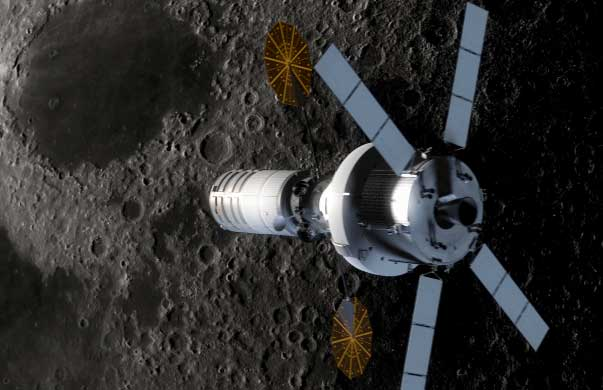
\includegraphics[width = 5.5in]{Figures/Cygnus_LunarStation.jpg}
		\label{Figure: Title Graphic}
		\end{figure}
        \        
        
        \Large
        AA 279D - Spacecraft Formation-Flying and Rendezvous\\
        Stanford University\\
        
    \end{center}
\end{titlepage}

% Update the revision history with each assignment
\section*{Revision History}

\begin{table}[ht]
    \centering
    % \caption{Summary of project revisions.}
    \begin{tabular}{ll}
        \toprule
        \textbf{Rev} & \textbf{Changes} \\
        \hline
        PS1 & \tabitem Created document \\
            & \tabitem Added problem set 1 material  \\
        \hline
        PS2 & \tabitem Fixed Excessive error between Numerical and Keplerian propogation \\
        & \tabitem Fixed errors in comparing RTN frames \\
            & \tabitem Added problem set 2 material  \\
        \hline
        PS3 & \tabitem Fixed mistake with manuver plots from PS2 \\
            & \tabitem Added problem set 3 material  \\
        \hline
        PS4 & \tabitem Fixed PS3 errors with eccentric ROE \\
            & \tabitem Added problem set 4 material  \\
  
        \hline
        PS5            & \tabitem Added problem set 5 material  \\
      
        \hline
        PS6 & \tabitem Fixed PS4 Material \\
            & \tabitem Added problem set 6 material  \\
                \hline
        PS7
            & \tabitem Added problem set 7 material  \\
                \hline
        PS8             & \tabitem Added problem set 8 material  \\
                \hline
        PS9 & \tabitem Complete clean up of project for final report\\
        \bottomrule
    \end{tabular}
    \label{table:revision history}
\end{table}

\newpage
\tableofcontents

\newpage
\listoffigures

\newpage
\listoftables

%%%%%%%%%%%%%%%%%%%%%%%%%%%%%%%
% SCOPE 
%%%%%%%%%%%%%%%%%%%%%%%%%%%%%%%
\newpage
\section{Scope}
This report covers the requirements for the AA279d Spacecraft Formation Flying and Rendezvous project. In the report, we examine the rendezvous phase of a mission with a deputy and a chief spacecraft, where the deputy attempts to bring itself close to the chief.

%%%%%%%%%%%%%%%%%%%%%%%%%%%%%%%
% PROBLEM SETS
%%%%%%%%%%%%%%%%%%%%%%%%%%%%%%%
\section{Problem Set 1}
\subsection{Problem 1: Your Mission, Your Challenge}

In this section of the report, we examine several different mission formats with the goal of choosing one to work on for the project.

\subsubsection{Mission 1: VISORS (VIrtual Super-resolution Optics with Reconfigurable Swarms)}

\paragraph{Mission Name and Operator:} VISORS, which is a multi-institution collaboration with the GN\&C subsystem developed and operated by Stanford's Space Rendezvous Laboratory.

\paragraph{Primary and Secondary Mission Objectives:}
\begin{itemize}
    \item Primary: Obtain images of active regions of the Sun's coronal area in the extreme ultraviolet spectrum with unprecedented resolution; with the goal of improving the current thermodynamic models of the solar corona.
    \item Secondary: Demonstrate capabilities of novel convex optimization-based model predictive control algorithms with no flight heritage, as well as higher accuracy autonomous control. 
\end{itemize}

\paragraph{Number and Type of Satellites:} 
Two 6U CubeSats, one of which contains the optical payload, and the other which contains the detector.

\paragraph{Absolute and Relative Orbit Parameters:}
\begin{itemize}
    \item Low Earth Orbit (LEO)
    \item Sun-synchronous orbit
    \item Therefore roughly: [$a = 6978$ km, $e = 0.001$, $i = 97.8^{\circ}$, $\Omega = \text{tbd}$, $\omega = \text{tbd}$, $M = \text{tbd}$]
    \item Relative configuration: Two spacecraft flying in formation with 40 meters separation, maintaining millimeter level accuracy.
    \item Launch date: Originally scheduled for October 2024 (now 2026)
    \item Mission duration: 100 observation attempts divided into 10 sets of 10 observations, with 2 weeks in standby mode between sets of observations.
\end{itemize}

\paragraph{Basic Description of Functioning/Scientific Principle:}
VISORS optics spacecraft has a photon sieve payload that uses constructive interference on a detector payload that's on the detector spacecraft to focus light. This creates a high contrast image with 0.1" resolution in the extreme ultraviolet. The spacecraft also has deployable solar panels that double as sunshade. These help block light coming from outside the area of interest.

\paragraph{Key DGN\&C Requirements:}
\begin{itemize}
    \item \textbf{Alignment with active region (pointing):} The center of the photon sieve must not deviate from the line connecting the center of the detector aperture and the target active region by more than 18 mm.
    \item \textbf{Line-of-sight stability/image drift:} The spacecraft's inertial relative velocity in the plane perpendicular to the line of sight must not exceed 0.2 mm/s, so common features can be tracked across exposures.
    \item \textbf{Focus:} The distance between the detector aperture center and the photon sieve pattern center must not deviate by more than 15 mm from the nominal separation of 40 m.
\end{itemize}

\paragraph{Classification of DSS:}
Formation-flying mission with high-precision relative positioning requirements.

\subsubsection{Mission 2: TanDEM-X (TerraSAR-X Add-on for Digital Elevation Measurement)}

\paragraph{Mission Name and Operator:} 
TanDEM-X, operated by the German Aerospace Center (DLR) and Airbus Defence and Space.

\paragraph{Primary and Secondary Mission Objectives:}
\begin{itemize}
    \item Primary: Generate a consistent global Digital Elevation Model (DEM) corresponding to the HRTE-3 model specifications with a relative vertical accuracy of 2 m for flat terrain and 4 m for steep terrain.
    \item Secondary: Demonstrate advanced SAR imaging techniques and interferometric satellite formation in space.
\end{itemize}

\paragraph{Number and Type of Satellites:} 
Two identical X-band radar satellites (TerraSAR-X and TanDEM-X).

\paragraph{Absolute and Relative Orbit Parameters:}
\begin{itemize}
    \item Sun-synchronous orbit at 514 km altitude
    \item 97.44$^{\circ}$ inclination
    \item 11-day repeat cycle (167 orbits)
    \item Eccentricity: 0.001
    \item Therefore roughly: [$a = 6892$ km, $e = 0.001$, $i = 97.44^{\circ}$, $\Omega = \text{tbd}$, $\omega = \text{tbd}$, $M = \text{tbd}$]
    \item Relative configuration: Helix formation with typical separation of 200-500 m
    \item Launch dates: TerraSAR-X (June 15, 2007), TanDEM-X (June 21, 2010)
    \item Mission duration: Initially 3 years, extended multiple times (still operational)
\end{itemize}

\paragraph{Basic Description of Functioning/Scientific Principle:}
TanDEM-X operates as a single-pass radar interferometer where two satellites fly in close formation, enabling bistatic SAR interferometry. By precisely measuring the phase difference between radar signals reflected from the Earth's surface to both satellites, the system creates highly accurate elevation maps. The tandem configuration enables highly accurate single-pass cross-track interferogram without the inherent accuracy limitation imposed by repeat pass interferometry due to decorrelation and atmospheric disturbances.

\paragraph{Key DGN\&C Requirements:}
\begin{itemize}
    \item Helix formation control with 150-500 m separation for collision avoidance
    \item Baseline determination with mm-level accuracy using GPS measurements
    \item Phase synchronization between radar instruments with accuracy of ~1º
    \item Automated formation-keeping with daily in-plane maneuvers
    \item Precise relative position knowledge to support bistatic interferometry
\end{itemize}

\paragraph{Classification of DSS:}
Formation-flying mission with meter-level relative positioning requirements.

\subsubsection{Mission 3: Starling}

\paragraph{Mission Name and Operator:} 
Starling, operated by NASA Ames Research Center with the Starling Formation-flying Optical eXperiment (StarFOX) operated by Stanford's Space Rendezvous Laboratory.

\paragraph{Primary and Secondary Mission Objectives:}
\begin{itemize}
    \item Primary: Demonstrate autonomous swarm technologies for distributed space systems, including swarm navigation, maneuver planning, communications and coordination.
    \item Secondary: Demonstrate technologies that enable multipoint science data collection by several small spacecraft flying in swarms.
\end{itemize}

\paragraph{Number and Type of Satellites:} 
Four identical 6U CubeSats built by Blue Canyon Technologies.

\paragraph{Absolute and Relative Orbit Parameters:}
\begin{itemize}
    \item Low Earth Orbit at approximately 550 km altitude
    \item Therefore roughly: [$a = 6928$ km, $e = 0.001$, $i = 97.8^{\circ}$, $\Omega = \text{tbd}$, $\omega = \text{tbd}$, $M = \text{tbd}$]
    \item Relative configuration: Variable distance formation from several kilometers to less than 1 km
    \item Launch date: July 17, 2023 on a Rocket Lab Electron vehicle from New Zealand
    \item Mission duration: Approximately 1 year
\end{itemize}

\paragraph{Basic Description of Functioning/Scientific Principle:}
The Starling mission tests four key technologies: (1) StarFOX (Starling Formation-flying Optical eXperiment), which uses onboard star tracker cameras for swarm navigation, (2) Distributed Spacecraft Autonomy (DSA), which enables the swarm to sense and react to the environment autonomously, (3) inter-satellite communications for networking between spacecraft, and (4) autonomous maneuver planning and execution. The StarFOX system uses an advanced algorithm that processes star tracker images to compute spacecraft orientation and visually detect and track other spacecraft in the swarm. These measurements are then shared between spacecraft, enabling the swarm to determine its position without relying on external navigation sources.

\paragraph{Key DGN\&C Requirements:}
\begin{itemize}
    \item Autonomous angles-only navigation using star tracker cameras
    \item Real-time inter-satellite communications to share measurement data
    \item Distributed orbit determination among all spacecraft
    \item Autonomous collision avoidance and maneuver planning
    \item Cooperative swarm decision-making without ground intervention
\end{itemize}

\paragraph{Classification of DSS:}
Swarm mission with autonomous coordination capabilities and moderate relative positioning requirements (meter to kilometer-level).

\subsubsection{Mission 4: SpaceX Dragon ISS Docking Mission}

\paragraph{Mission Name and Operator:} 
SpaceX Crew Dragon ISS Docking Mission, operated by SpaceX in partnership with NASA.

\paragraph{Primary and Secondary Mission Objectives:}
\begin{itemize}
    \item Primary: Transport crew and/or cargo to and from the International Space Station
    \item Secondary: Demonstrate autonomous rendezvous and docking capabilities
\end{itemize}

\paragraph{Number and Type of Satellites:} 
Two spacecraft (Dragon capsule and International Space Station).

\paragraph{Absolute and Relative Orbit Parameters:}
\begin{itemize}
    \item ISS orbit: $\sim$400-420 km altitude
    \item 51.6° inclination
    \item 90-minute orbital period
    \item Therefore roughly: [$a = 6780$ km, $e = 0.0006$, $i = 51.6^{\circ}$, $\Omega = \text{tbd}$, $\omega = \text{tbd}$, $M = \text{tbd}$]
    \item Relative configuration: Approach from phasing orbit to final docking
    \item Launch dates: Multiple missions since 2020 (Demo-2, Crew-1, Crew-2, ..., Crew-10)
    \item Mission duration: Typically 6 months for crew rotation missions
\end{itemize}

\paragraph{Basic Description of Functioning/Scientific Principle:}
The Dragon spacecraft performs a multi-phase rendezvous with the ISS, including initial phasing, height adjustment maneuvers, coelliptic approach, proximity operations, and final docking. The vehicle uses a combination of absolute and relative navigation sensors to guide it from the initial orbital insertion to the final soft-capture and hard-capture with the ISS docking adapter. The mission requires precise coordination between the approaching vehicle and the target space station.

\paragraph{Key DGN\&C Requirements:}
\begin{itemize}
    \item Far-field rendezvous using absolute navigation (GPS)
    \item Near-field proximity operations using relative navigation (lidar, cameras)
    \item Centimeter-level precision for final docking phase
    \item Autonomous trajectory planning with collision avoidance capabilities
    \item Real-time fault detection and response
    \item Precise attitude control during all mission phases
\end{itemize}

\paragraph{Classification of DSS:}
Rendezvous and docking mission with extremely high precision requirements in the final approach phase (cm-level positioning, mm-level rates).

\subsubsection{Selected Mission for Course Project}
From these candidates, we selected the \textbf{SpaceX Dragon ISS Docking Mission} as the framework for the course project. This was chosen due to our desire to work on the rendezvous problem.

\subsection{Orbit Simulation, Review of Astrodynamics}
\subsubsection{Initial Orbital Elements}

\begin{table}[H]
    \centering
    \begin{tabular}{cccccc} \hline
        $a$ (m) & $e$ & $i$ (deg) & $\Omega$ (deg) & $\omega$ (deg) & $M$ (deg) \\ \hline 
         6780000 & 0.0006 & 51.6 & 0 & 0 & 0 \\ \hline
    \end{tabular}
    \caption{Initial classical orbit elements for the ISS/Dragon mission}
    \label{tab:iss_ics}
\end{table}

\subsubsection{Initial Position and Velocity in ECI Frame}
\begin{align}
    \vec{r}_{ECI} &= [6775932.00, 0.00, 0.00]^T \text{ m} \\
    \vec{v}_{ECI} &= [0.00, 4765.51, 6012.58]^T \text{ m/s}
\end{align}

\subsubsection{Numerical Integration Results}

\begin{figure}[H]
    \centering
    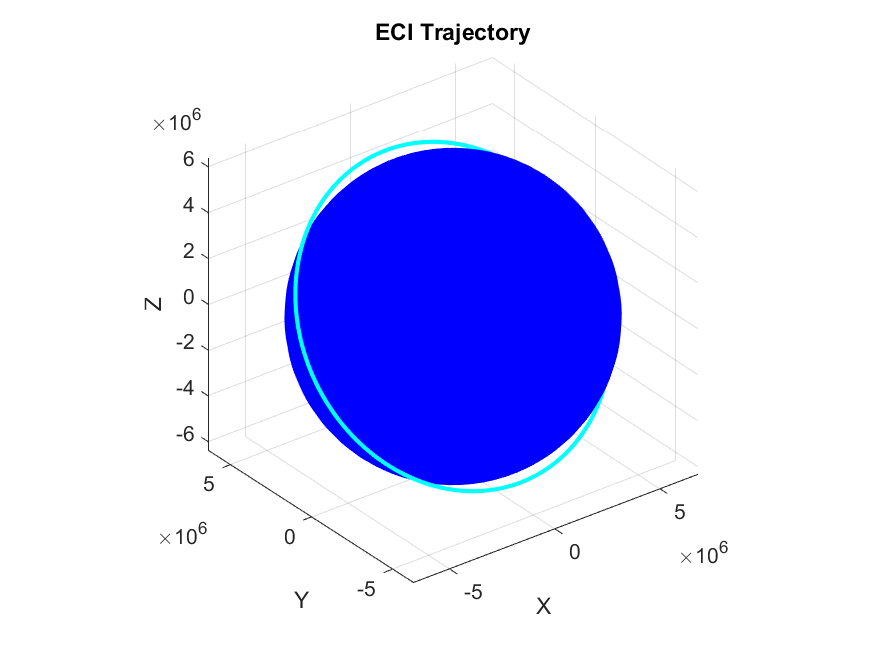
\includegraphics[width=0.5\textwidth]{PS1/Figures/eci_trajectory_unperturbed.png}
    \caption{ECI trajectory without J2 perturbation}
    \label{fig:eci_unperturbed}
\end{figure}

\begin{figure}[H]
    \centering
    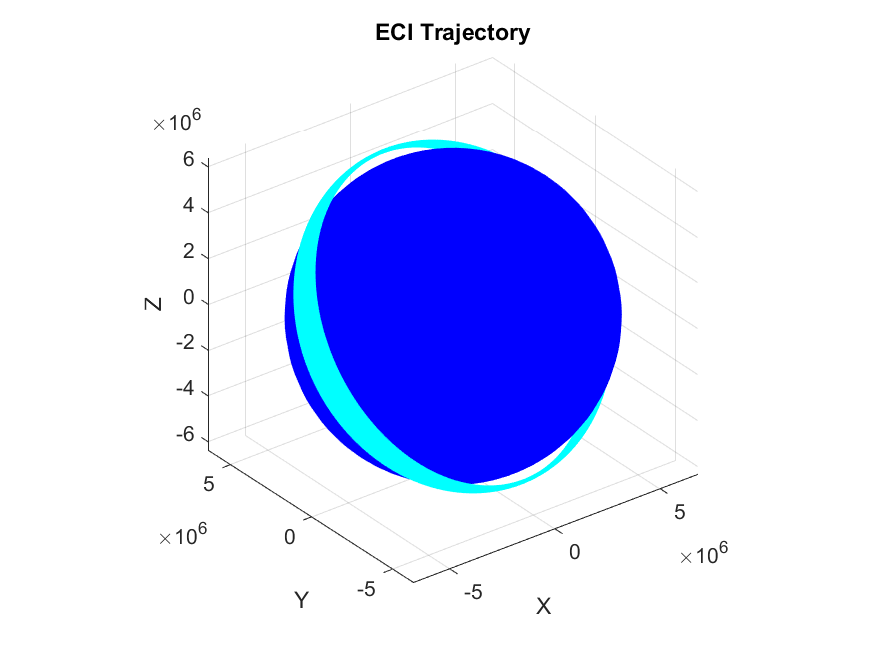
\includegraphics[width=0.5\textwidth]{PS1/Figures/eci_trajectory_j2.png}
    \caption{ECI trajectory with J2 perturbation}
    \label{fig:eci_j2}
\end{figure}

The J2-perturbed trajectory shows a slight precession of the orbital plane, visible as a spreading of the trajectory when compared to the unperturbed case.

\subsubsection{Verification of Numerical Integration}

\begin{figure}[H]
    \centering
    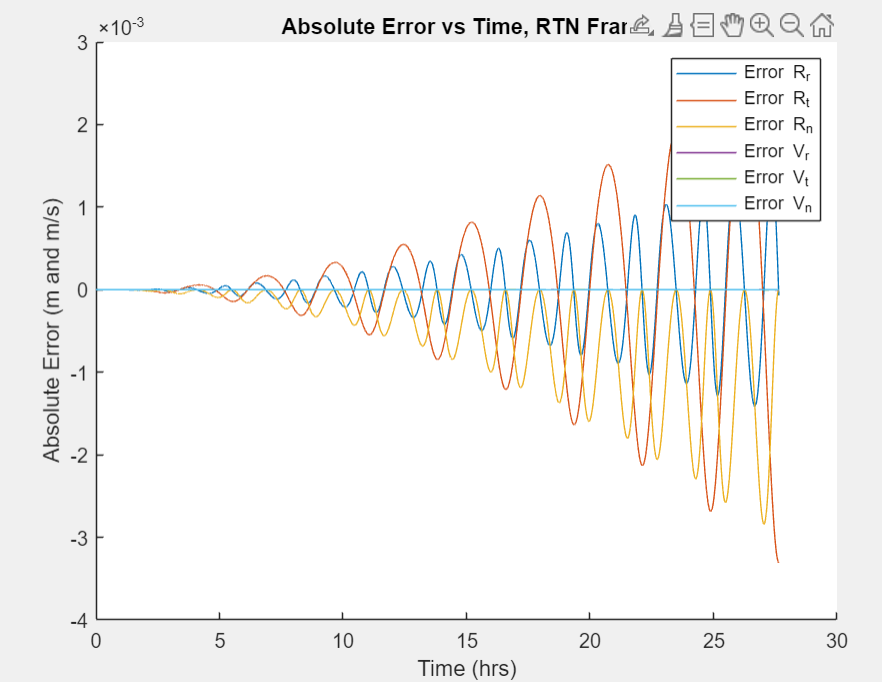
\includegraphics[width=0.5\textwidth]{PS1/Figures/error_comparison.png}
    \caption{Position and velocity errors between numerical integration and analytical solution in RTN frame}
    \label{fig:error_comparison}
\end{figure}

The error comparison shows differences growing to several kilometers over the simulation period, showing accumulated numerical integration errors as expected.

\subsubsection{Orbital Elements and Conservation Properties}

\begin{figure}[H]
    \centering
    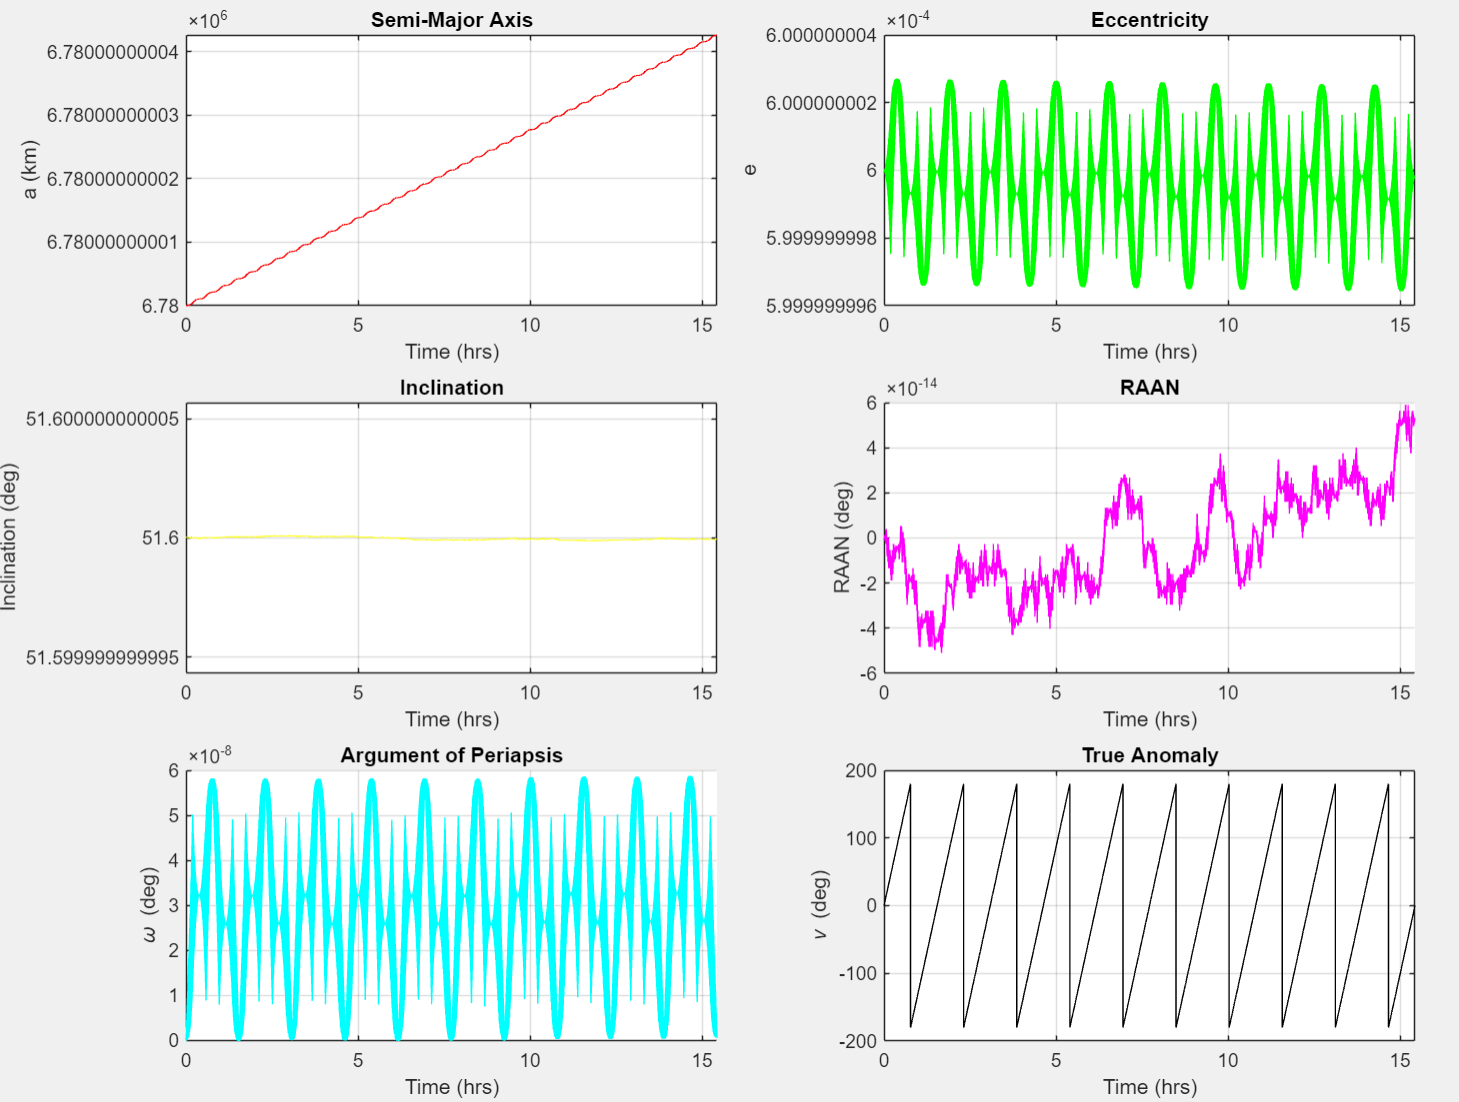
\includegraphics[width=0.5\textwidth]{PS1/Figures/orbital_elements_unperturbed.png}
    \caption{Osculating orbital elements without J2 perturbation}
    \label{fig:oe_unperturbed}
\end{figure}

\begin{figure}[H]
    \centering
    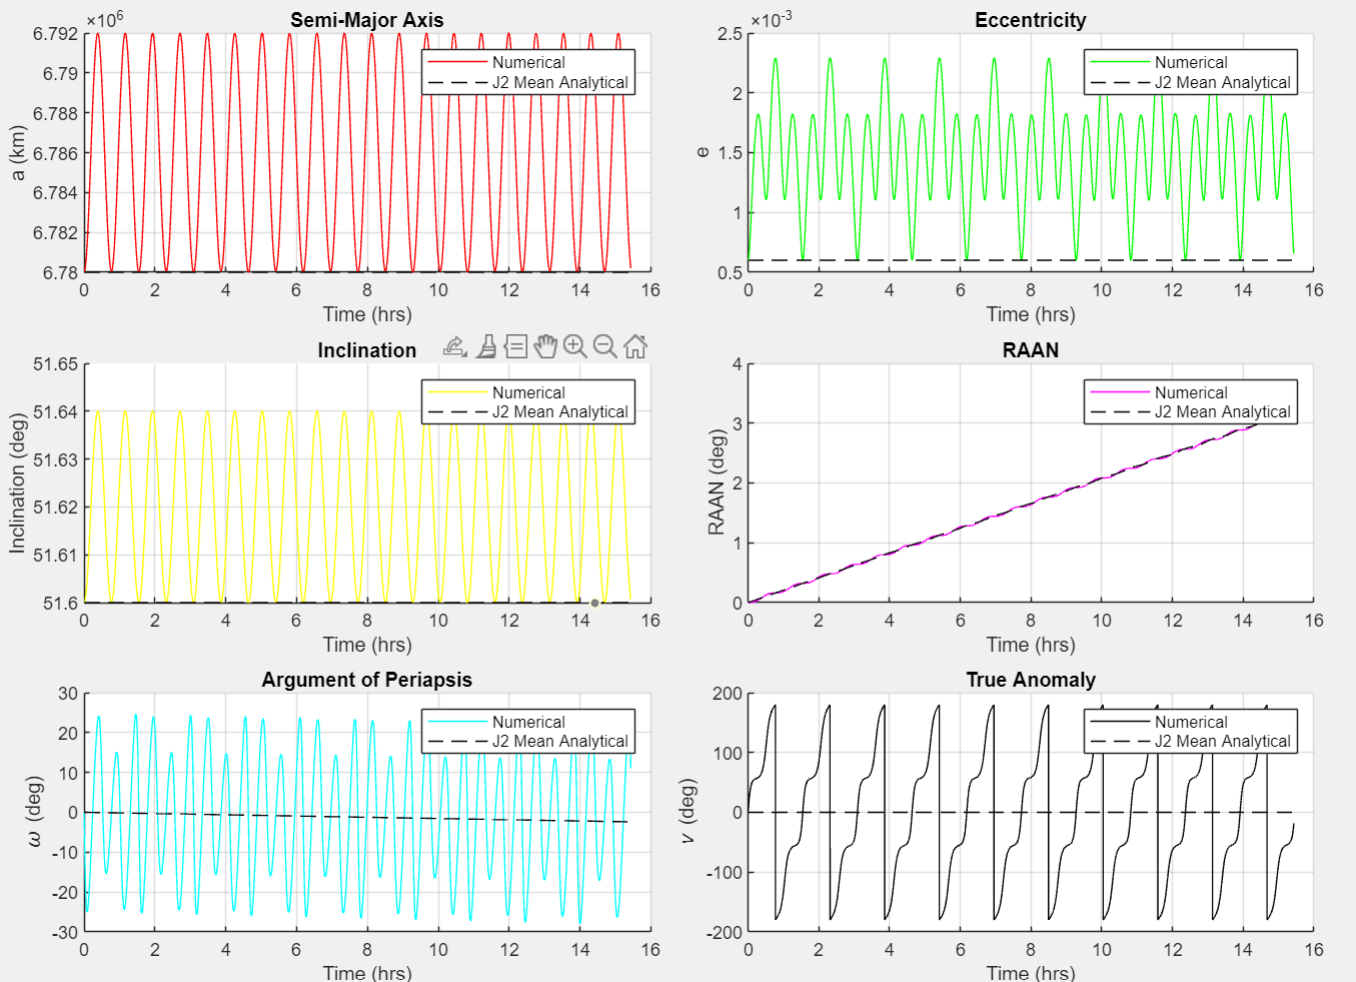
\includegraphics[width=0.5\textwidth]{PS1/Figures/orbital_elements_j2.png}
    \caption{Osculating orbital elements with J2 perturbation}
    \label{fig:oe_j2}
\end{figure}

\begin{figure}[H]
    \centering
    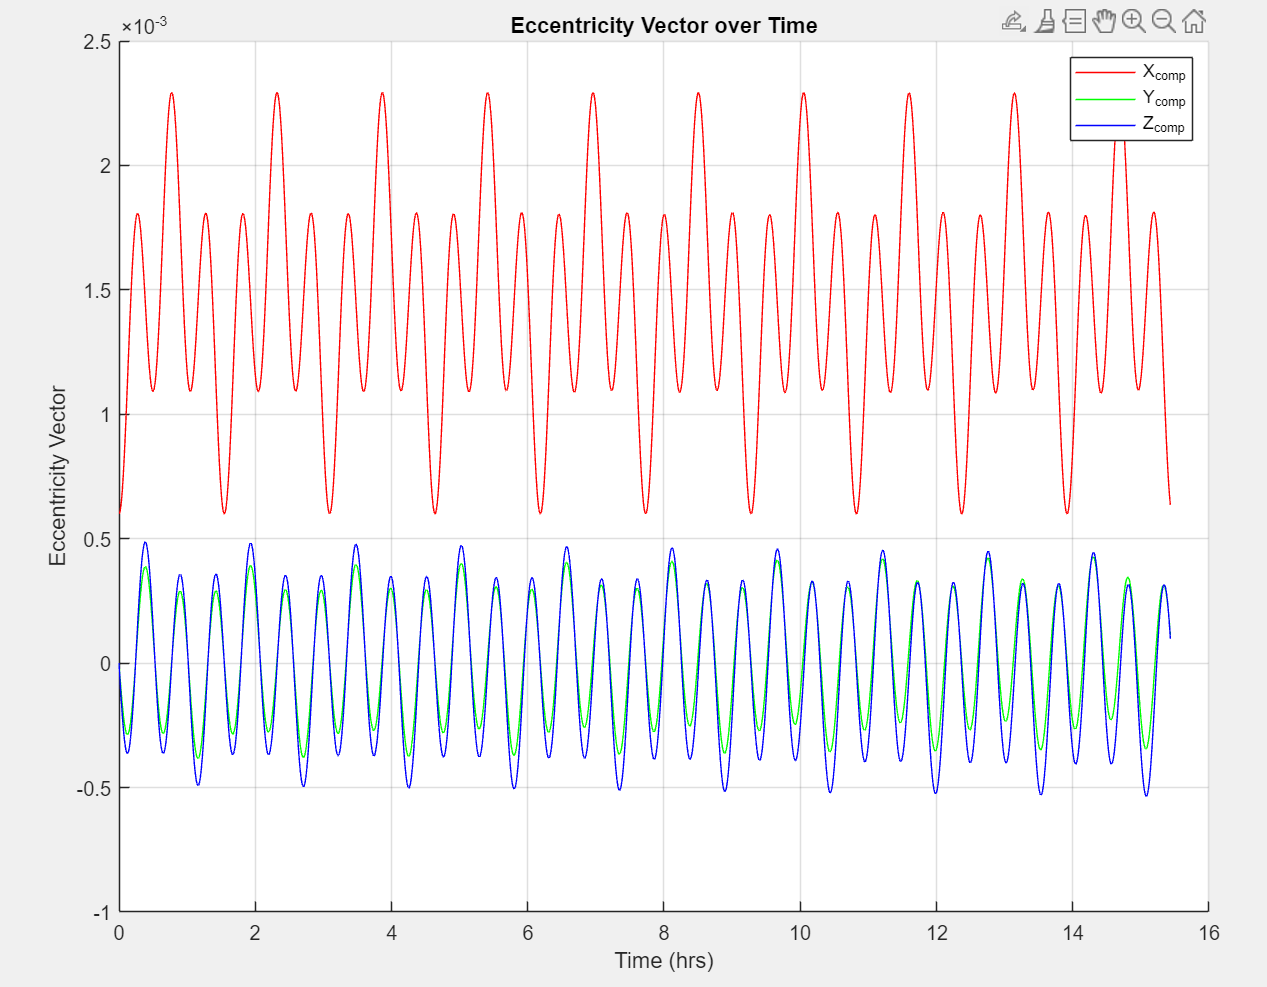
\includegraphics[width=0.5\textwidth]{PS1/Figures/eccentricity_vector_j2.png}
    \caption{Eccentricity vector components over time with J2 perturbation}
    \label{fig:ecc_vector}
\end{figure}

\begin{figure}[H]
    \centering
    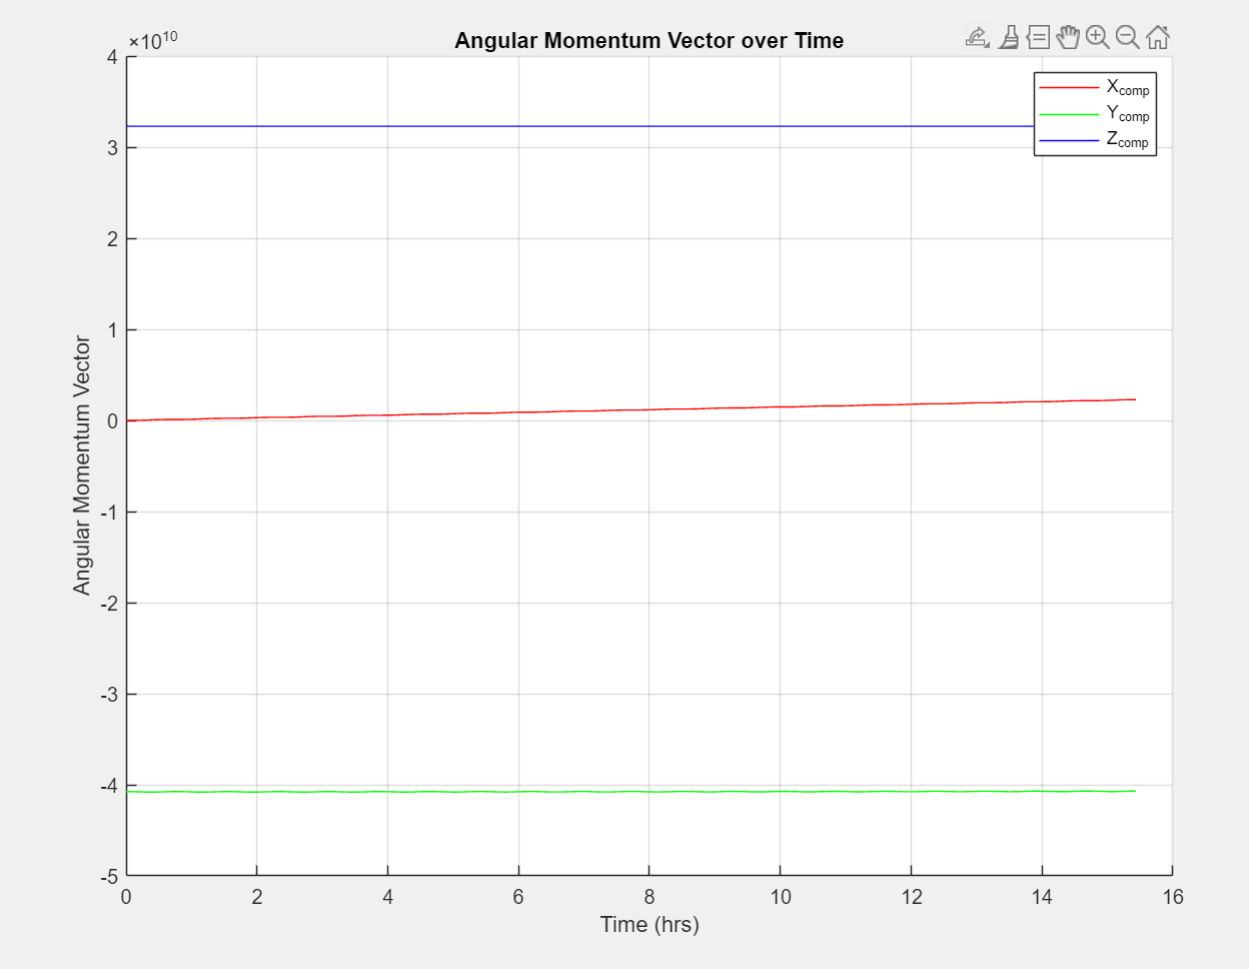
\includegraphics[width=0.5\textwidth]{PS1/Figures/angular_momentum_j2.png}
    \caption{Angular momentum vector components over time with J2 perturbation}
    \label{fig:ang_mom}
\end{figure}

\begin{figure}[H]
    \centering
    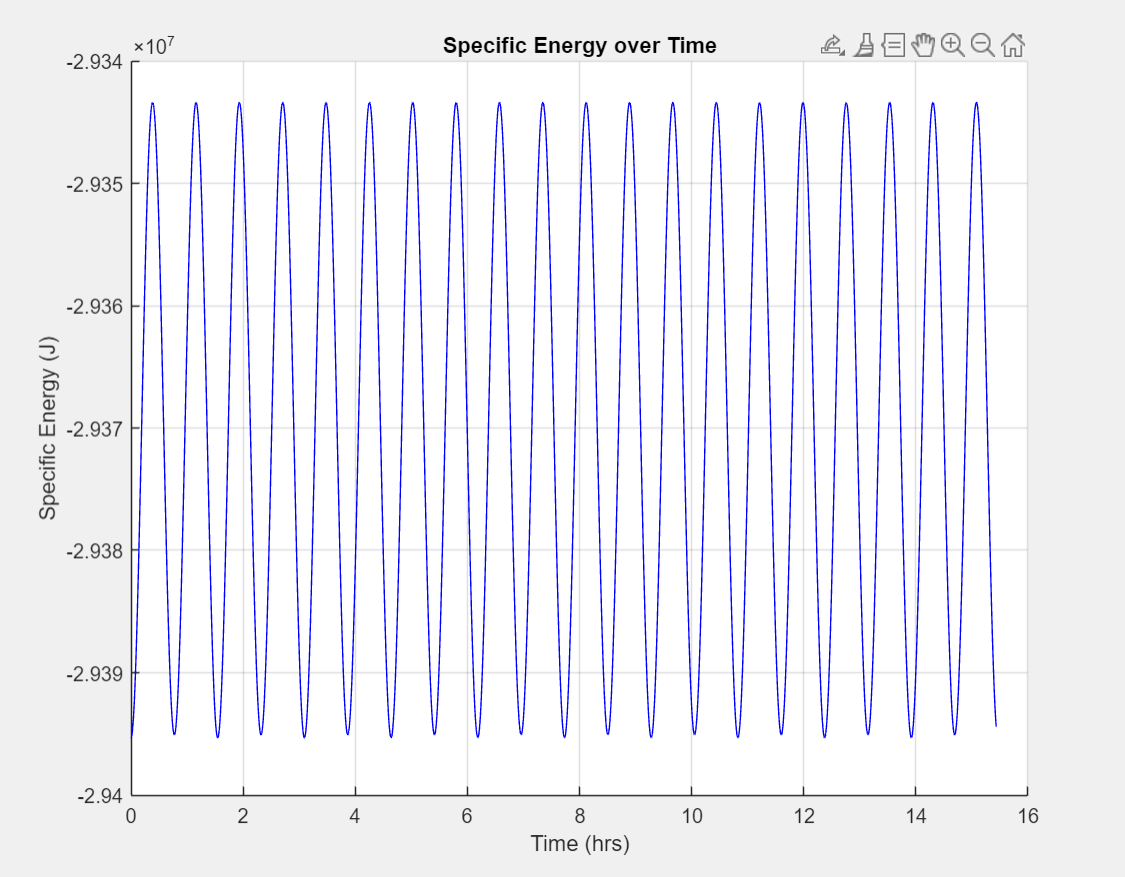
\includegraphics[width=0.5\textwidth]{PS1/Figures/specific_energy_j2.png}
    \caption{Specific mechanical energy over time with J2 perturbation}
    \label{fig:energy}
\end{figure}

In the unperturbed case (Figure \ref{fig:oe_unperturbed}), while we expect perfect conservation of orbital elements, some minor variations are observed due to numerical integration effects. In the J2-perturbed case (Figure \ref{fig:oe_j2}), semi-major axis and eccentricity show small oscillations but no secular trends, while RAAN and argument of periapsis exhibit clear secular drifts, with RAAN decreasing and argument of periapsis increasing. The angular momentum vector (Figure \ref{fig:ang_mom}) changes direction but maintains nearly constant magnitude.

\subsubsection{Mean Elements and Analytical J2 Effects}
In Figure \ref{fig:oe_j2}, the dashed lines show the analytical mean element solutions for RAAN and argument of periapsis. The mean elements follow linear trends that closely match the average behavior of the osculating elements, showing our J2 secular effects.

\subsubsection{Reconciliation of Osculating and Mean Elements}
To reconcile the difference between osculating and mean elements we must consider the fact that numerical integration takes in osculating elements, while the analytical solution to J2 takes in mean elements. Therefore, if the same inputs are used for both, the results will be slightly off. To fix this, the Brouwer transform could be applied to the starting elements.

\newpage
\section{Problem Set 2}

\subsection{Everything is Relative}

\subsubsection{Initial Conditions}
For this problem, we use the ISS orbit parameters from Problem Set 1 for the chief spacecraft, and apply small variations to create the deputy spacecraft's initial state:

\begin{table}[H]
    \centering
    \begin{tabular}{ccc} \hline
        \textbf{Parameter} & \textbf{Chief} & \textbf{Deputy} \\ \hline 
        Initial position (RTN) [m] & [0, 0, 0] & [0, 0, 0] \\
        Initial velocity (RTN) [m/s] & [0, 0, 0] & [1, 1, 0] \\ \hline
    \end{tabular}
    \caption{Initial conditions for chief and deputy spacecraft in RTN frame}
    \label{tab:relative_ics}
\end{table}

The deputy begins at the same position as the chief but with a 1 m/s velocity offset in both the tangential and normal directions.

\subsubsection{Nonlinear Equations of Relative Motion}

\begin{figure}[H]
    \centering
    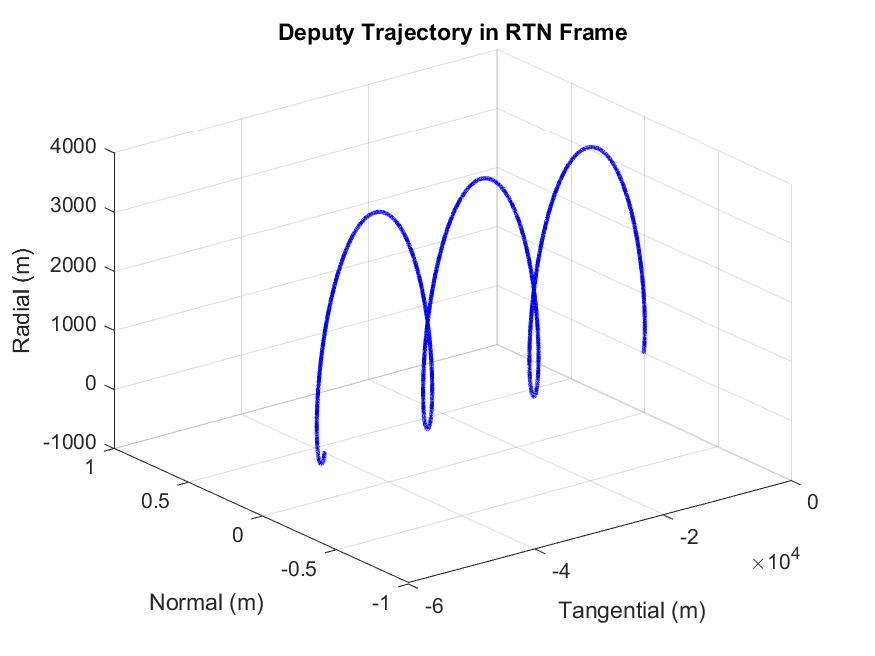
\includegraphics[width=0.7\textwidth]{PS2/Figures/Case1_RelativeTrajectory.png}
    \caption{Deputy trajectory in RTN frame from nonlinear equations of relative motion}
    \label{fig:relative_trajectory}
\end{figure}

\begin{figure}[H]
    \centering
    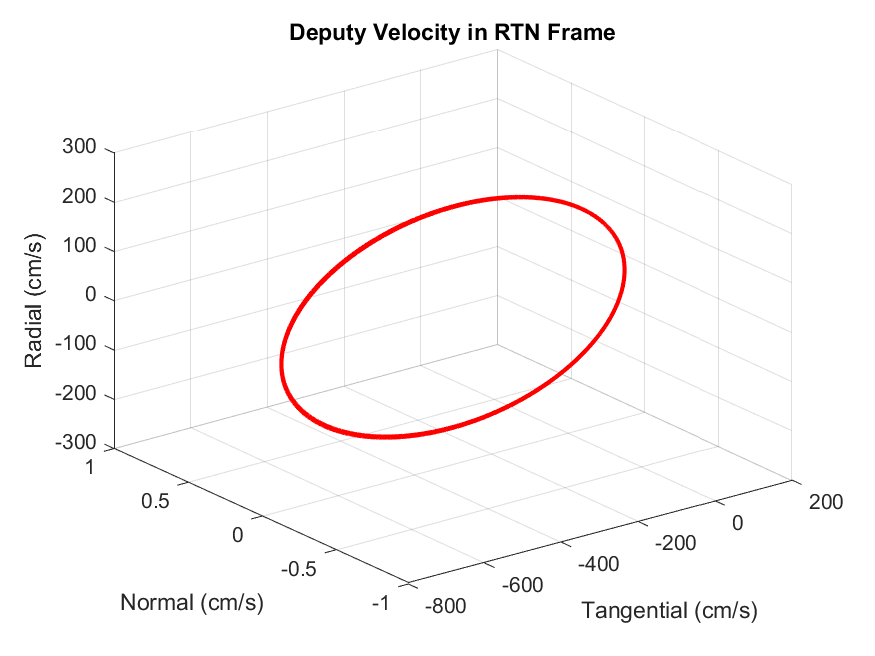
\includegraphics[width=0.7\textwidth]{PS2/Figures/Case1_RelativeVelocity.png}
    \caption{Deputy velocity in RTN frame from nonlinear equations of relative motion}
    \label{fig:relative_velocity}
\end{figure}

\subsubsection{Comparison of Methods}

\begin{figure}[H]
    \centering
    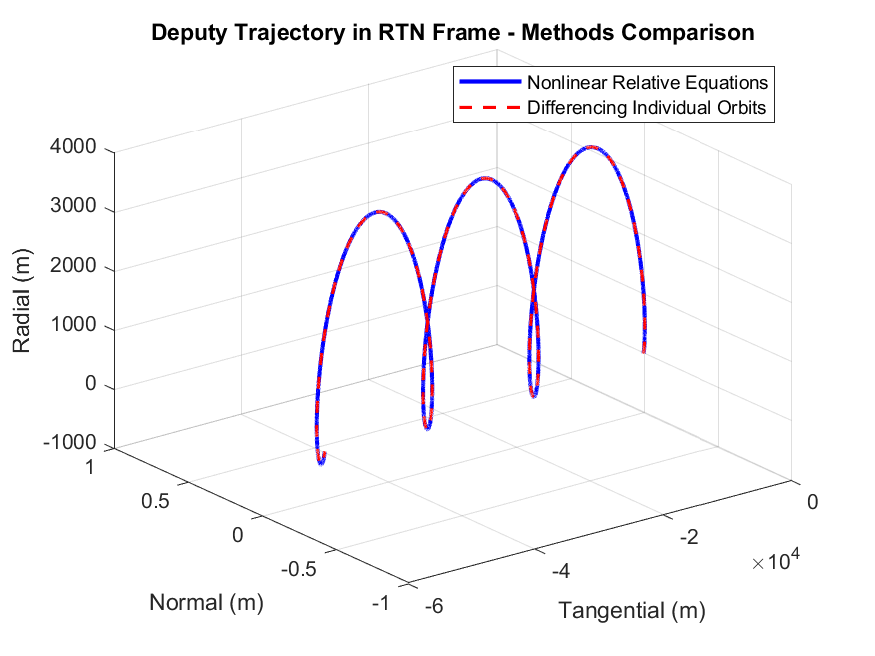
\includegraphics[width=0.7\textwidth]{PS2/Figures/Case1_MethodsComparison.png}
    \caption{Comparison of relative motion computed using nonlinear equations vs. differencing individual orbits}
    \label{fig:methods_comparison}
\end{figure}

\begin{figure}[H]
    \centering
    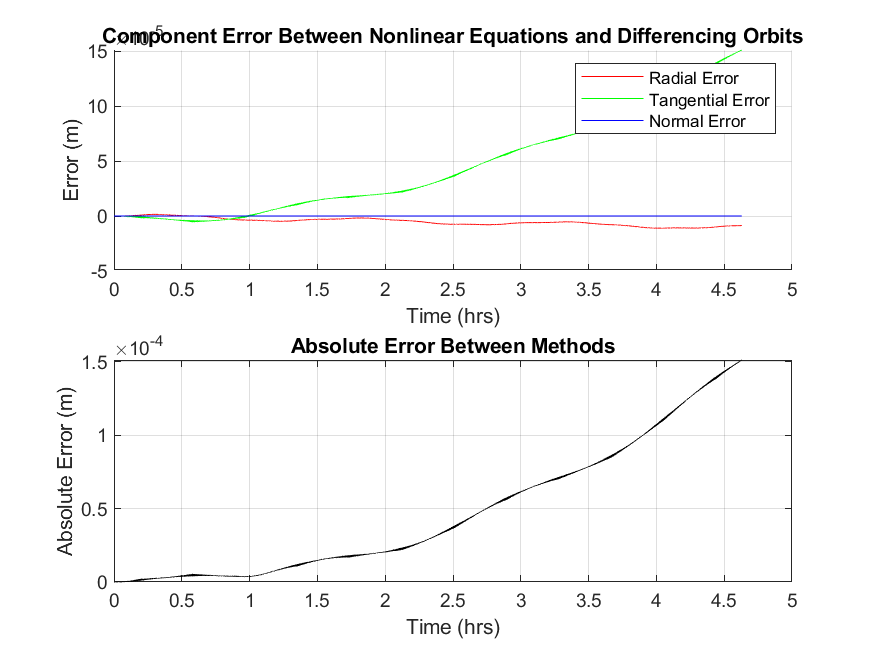
\includegraphics[width=0.7\textwidth]{PS2/Figures/Case1_MethodsError.png}
    \caption{Error between the two methods of computing relative motion}
    \label{fig:methods_error}
\end{figure}

Both methods produce nearly identical results, with maximum errors less than 0.2 mm and mean errors less than 0.05 mm, confirming their mathematical equivalence.

\subsubsection{Effect of Non-Zero Difference in Semi-Major Axis}

When a non-zero difference in semi-major axis is introduced by adding a 1 m/s tangential velocity component to the deputy, in addition to a 1 m/s radial velocity at the start of the simulation, there is drift:

\begin{figure}[H]
    \centering
    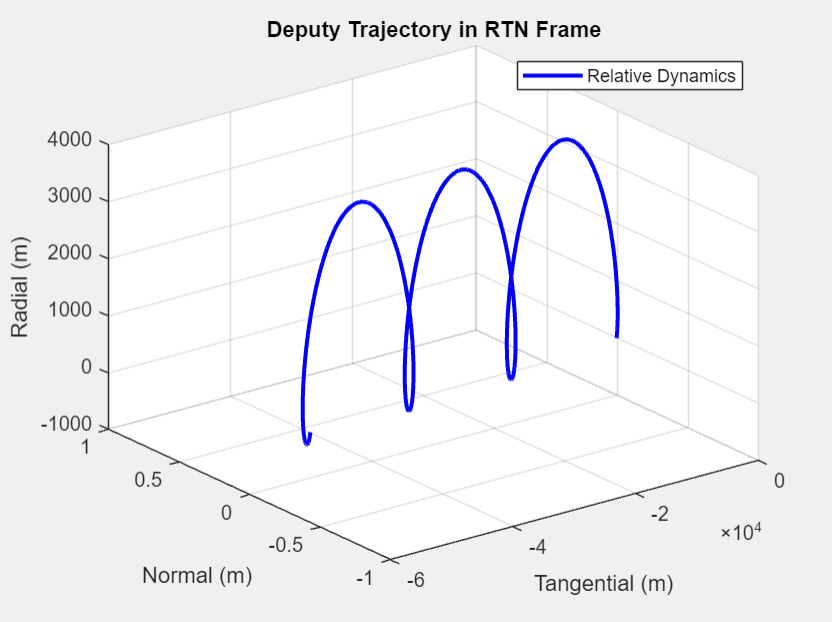
\includegraphics[width=0.7\textwidth]{PS2/Figures/Screenshot 2025-04-16 232749.png}
    \caption{Drifting Orbit}
    \label{fig:drift_comparison}
\end{figure}


\subsubsection{Re-establishing Bounded Motion}

To re-establish bounded periodic motion, we need to eliminate the semi-major axis difference through an impulsive maneuver. The most fuel-efficient approach is a tangential impulse at either apogee or perigee. Our code determines which is more efficent, and applies the manuver at that given point. The results are shown below:

\begin{figure}[H]
    \centering
    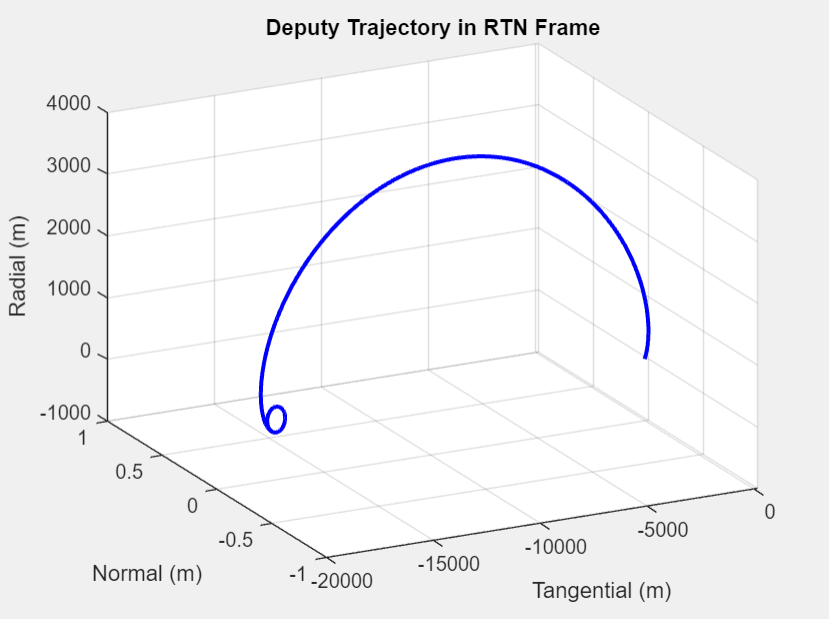
\includegraphics[width=0.7\textwidth]{PS2/Figures/Screenshot 2025-04-16 231907.png}
    \caption{Relative trajectory before and after corrective maneuver}
    \label{fig:maneuver_comparison1}
\end{figure}

\begin{figure}[H]
    \centering
    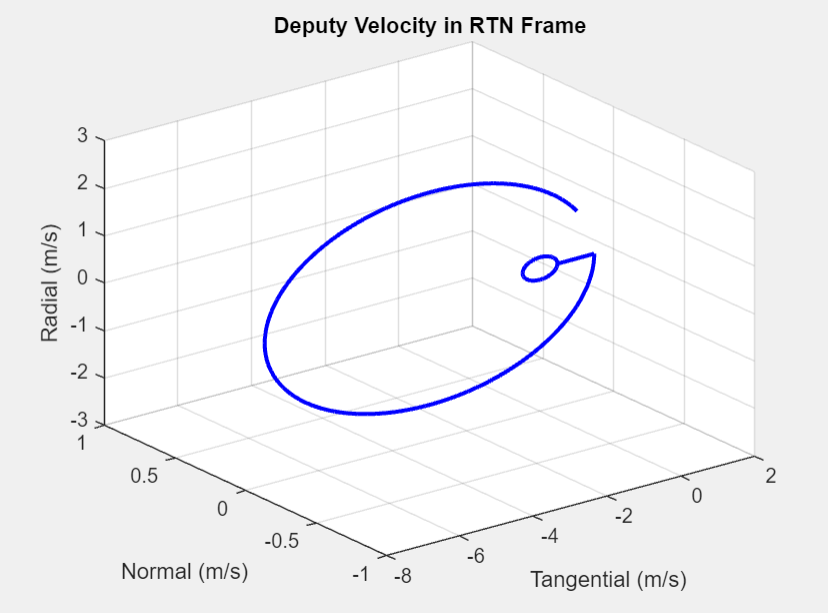
\includegraphics[width=0.7\textwidth]{PS2/Figures/Screenshot 2025-04-16 231937.png}
    \caption{Relative velocity before and after corrective maneuver}
    \label{fig:maneuver_comparison2}
\end{figure}

Analysis of the optimal maneuver:
\begin{itemize}
    \item Maneuver location: Perigee (minimum radius)
    \item Delta-v magnitude: 1.0054 m/s
    \item Maneuver time: 4.29 hours from simulation start
\end{itemize}

This tangential impulse at perigee equalizes the semi-major axes between the chief and deputy, re-establishing bounded relative motion as shown by the post-maneuver trajectory in Figure \ref{fig:maneuver_comparison}. The maneuver is optimal because it changes the orbit energy (and thus semi-major axis) most efficiently by applying thrust in the velocity direction at the point of maximum orbital velocity.

After the maneuver, bounded relative motion is achieved.

\newpage
\section{Problem Set 3}

\subsection{We are Close in Near-Circular Orbits}

\subsubsection{Initial Conditions}
For this problem, we set the initial conditions in classical orbital elements to be [6780000, 0.001, 0, 0, 0, 0]. This provides us with a near circular orbit that is sufficiently far from the attractor's center.

\subsubsection{Initial Conditions in ECI and RTN}
Inertial position and velocity of chief: [6773200, 0, 0, 0, 7700, 0]\\
RTN position and velocity of deputy: [0, 10, 0, 1, 0, 0]

\subsubsection{Integration Constants}

Using the HCW equations, we can find the integration constants based on these initial conditions: [0.0013, 0.0001, -0.0013, -0.0003, 0, 0]

\subsubsection{Propogation with HCW Equations}

\begin{figure}[H]
    \centering
    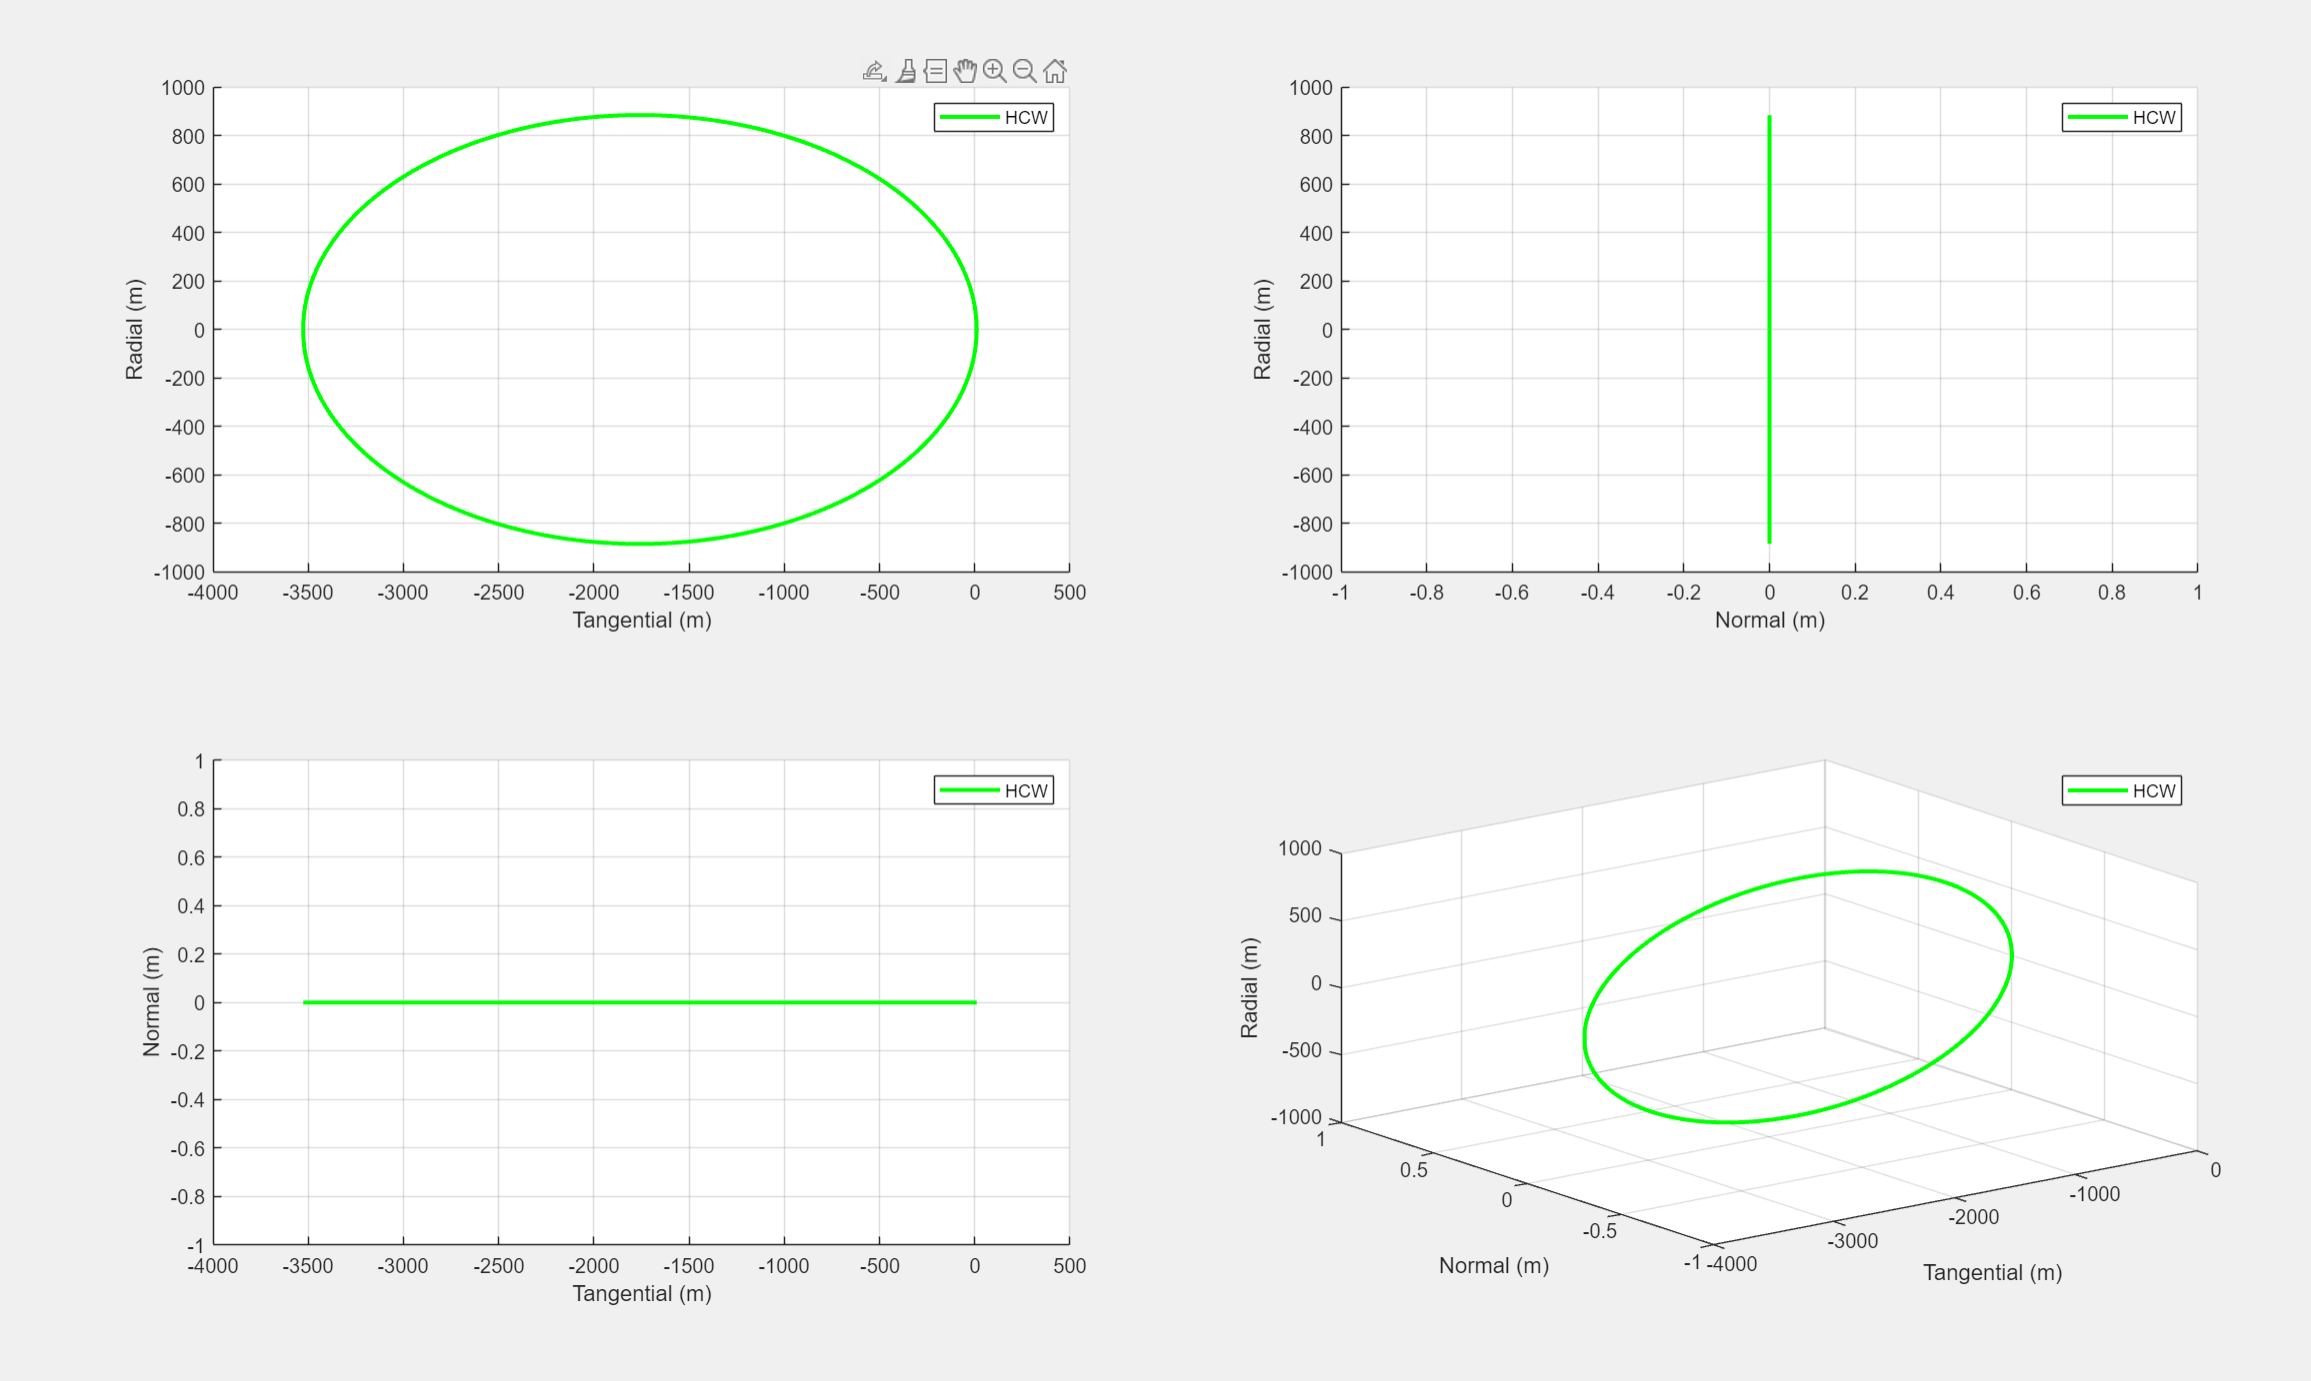
\includegraphics[width=0.7\textwidth]{PS3/Figures/HCW_Position.png}
    \caption{Deputy trajectory in RTN frame from HCW Equations}
    \label{fig:hcw_position}
\end{figure}

\begin{figure}[H]
    \centering
    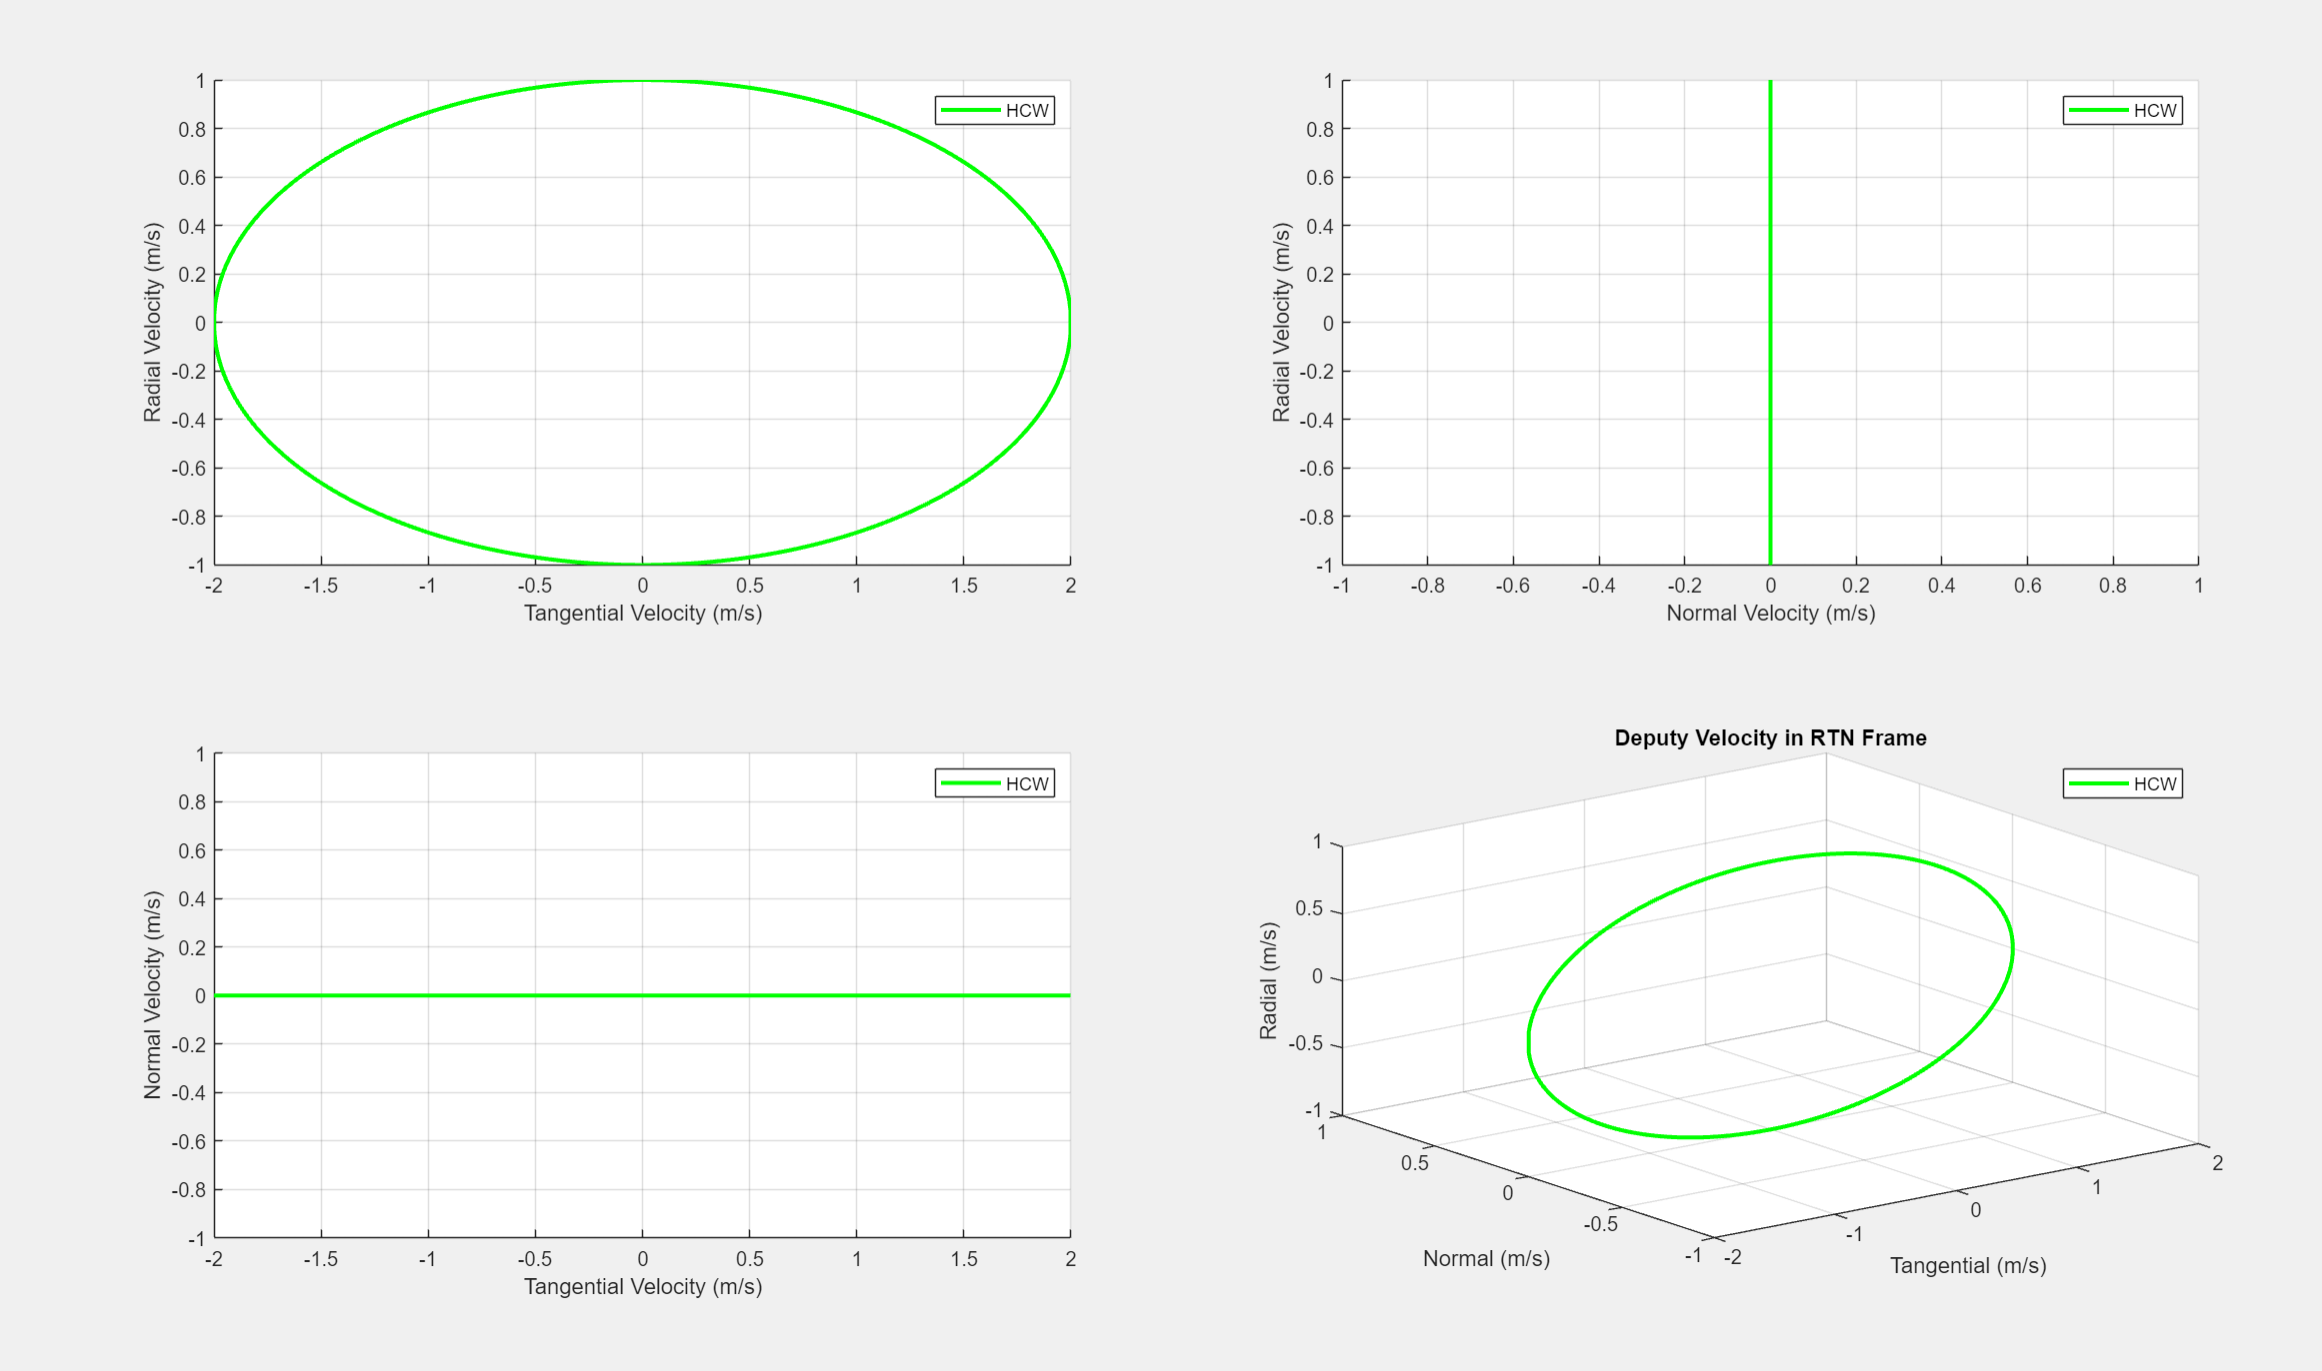
\includegraphics[width=0.7\textwidth]{PS3/Figures/HCW_Velocity.png}
    \caption{Deputy velocity in RTN frame from HCW Equations}
    \label{fig:hcw_velocity}
\end{figure}

\subsubsection{Expected Behavior}

The behavior we see in these plots aligns with expectations. Since the initial conditions involve a difference in the along track direction, with a radial velocity difference, there is no semi major axis difference, and therefore no energy difference, between the orbits. Thus, as expected, we see bounded relative motion with no drift.

\subsection{We are Close in Eccentric Orbits}

\subsubsection{Initial Conditions}
For this problem, we set the initial conditions of the chief in classical orbital elements to be [6780000, 0.1, 0, 0, 0, 0]. This provides us with an eccentric orbit that is sufficiently far from the attractor's center.\\

We set the initial conditions of the deputy to be [0, 10, 0, 1, 0, 0] in RTN as we did for the above problem. This again will give us bounded motion due to the equal energies of the deputy and chief.

\subsubsection{Integration Constants}
We find the integration constants to be: [0, 0.0001072, 0, -0.0002236, 0, 0]

\subsubsection{Propogation with YA Equations}

\begin{figure}[H]
    \centering
    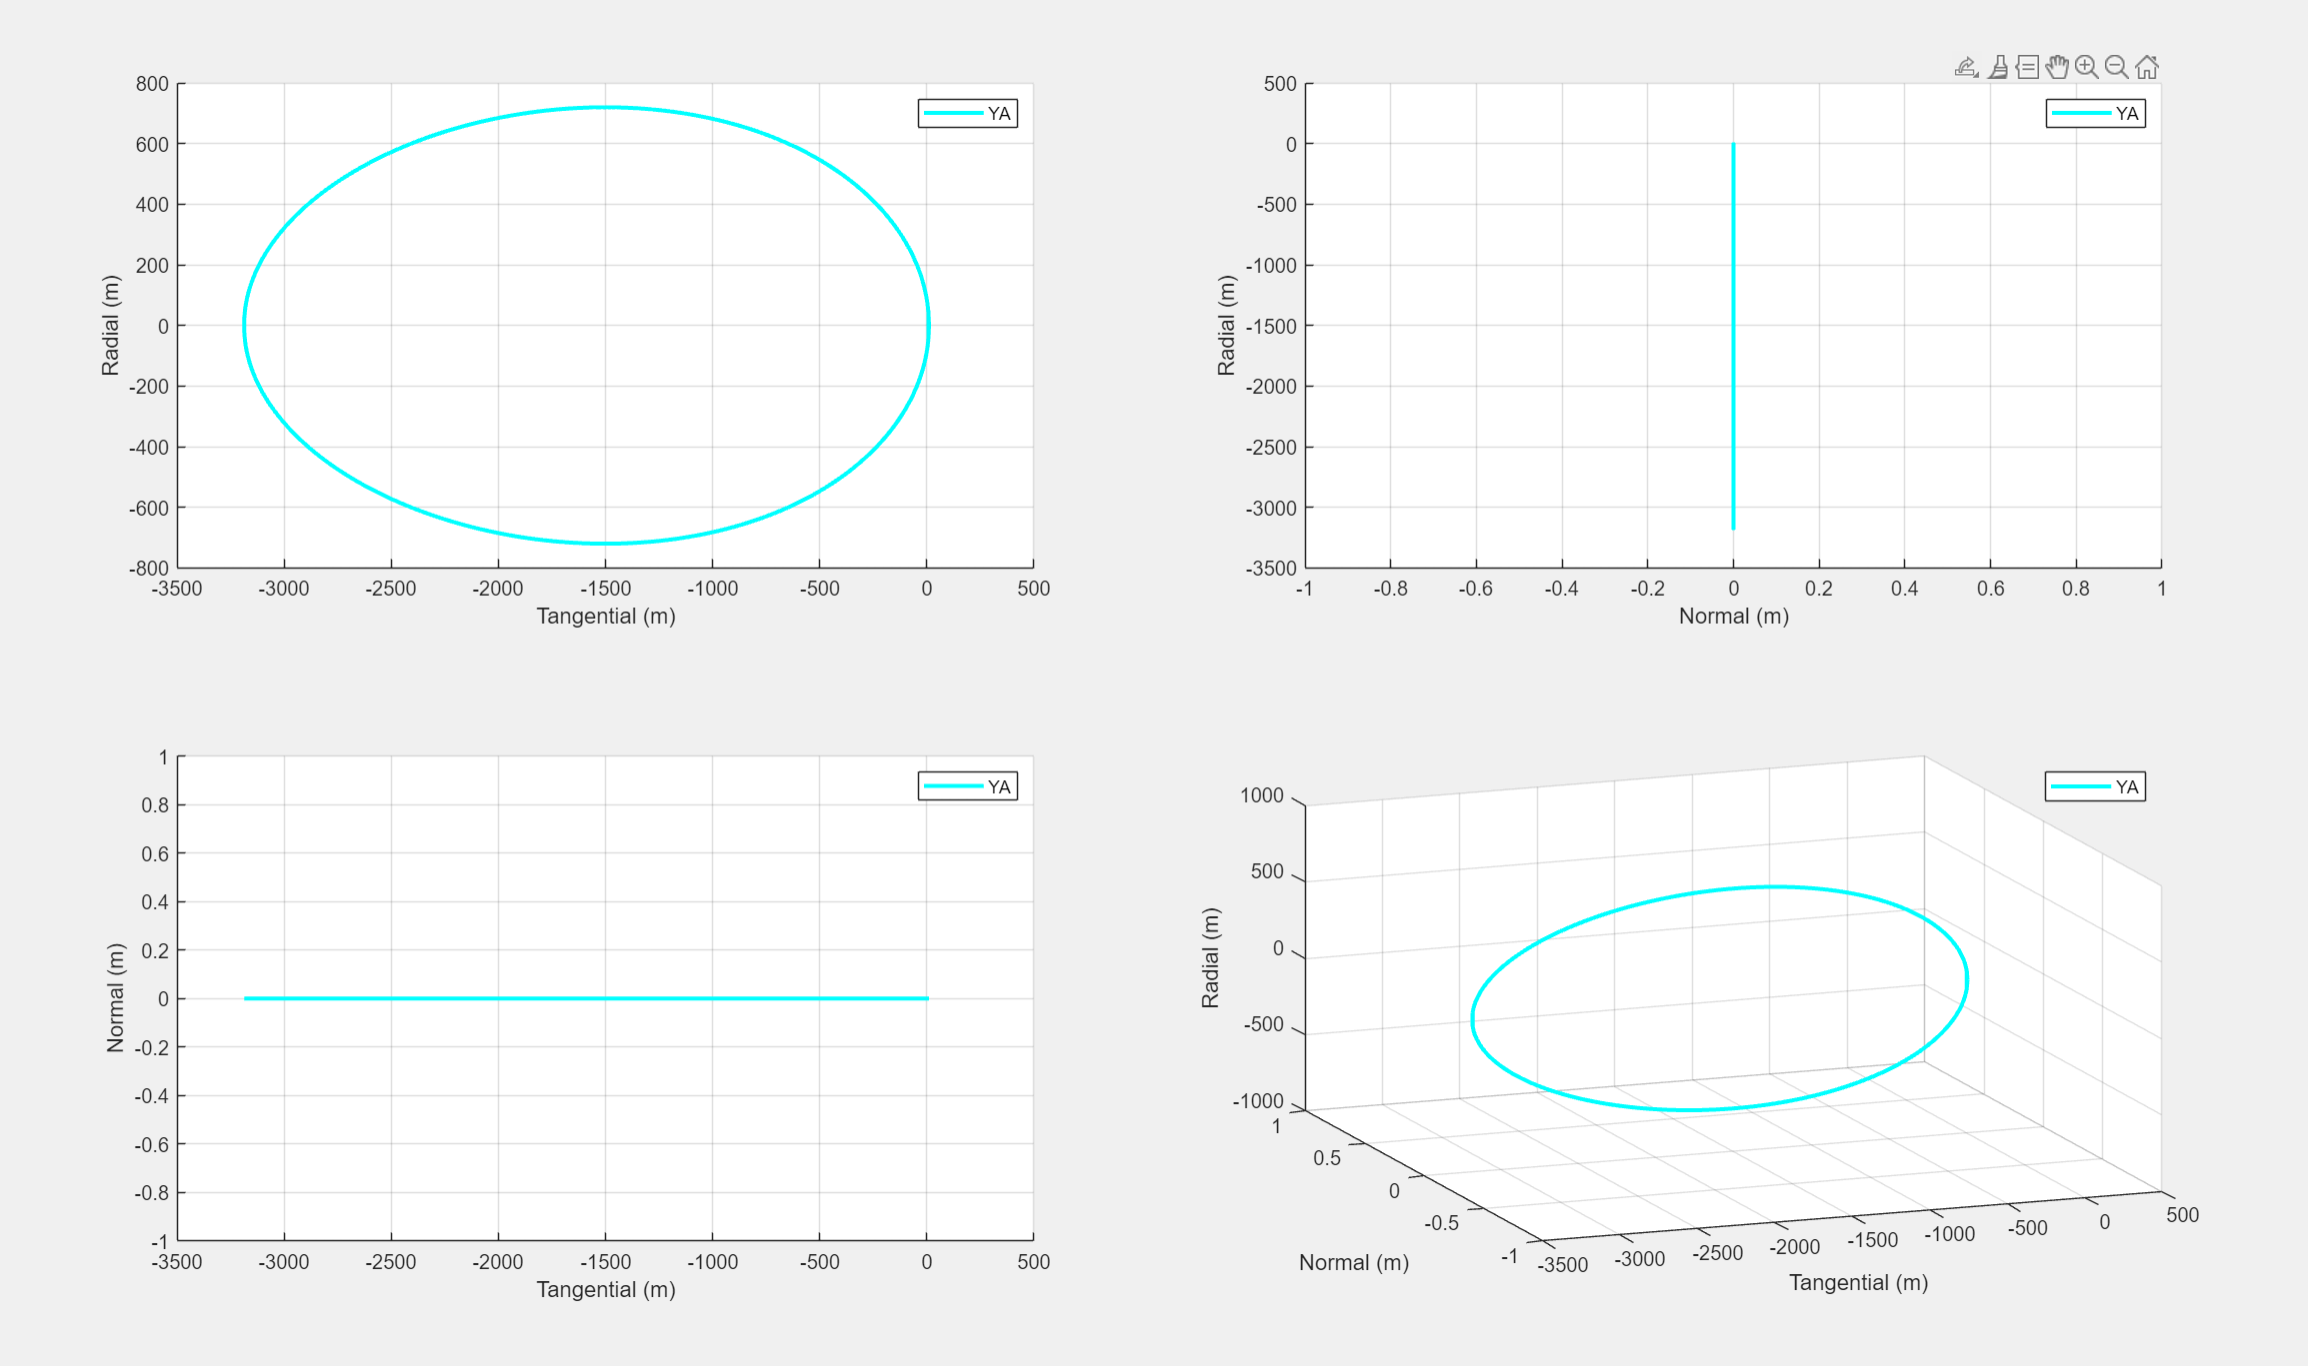
\includegraphics[width=0.7\textwidth]{PS3/Figures/YA_position.png}
    \caption{Deputy trajectory in RTN frame from YA Equations}
    \label{fig:ya_position}
\end{figure}

\begin{figure}[H]
    \centering
    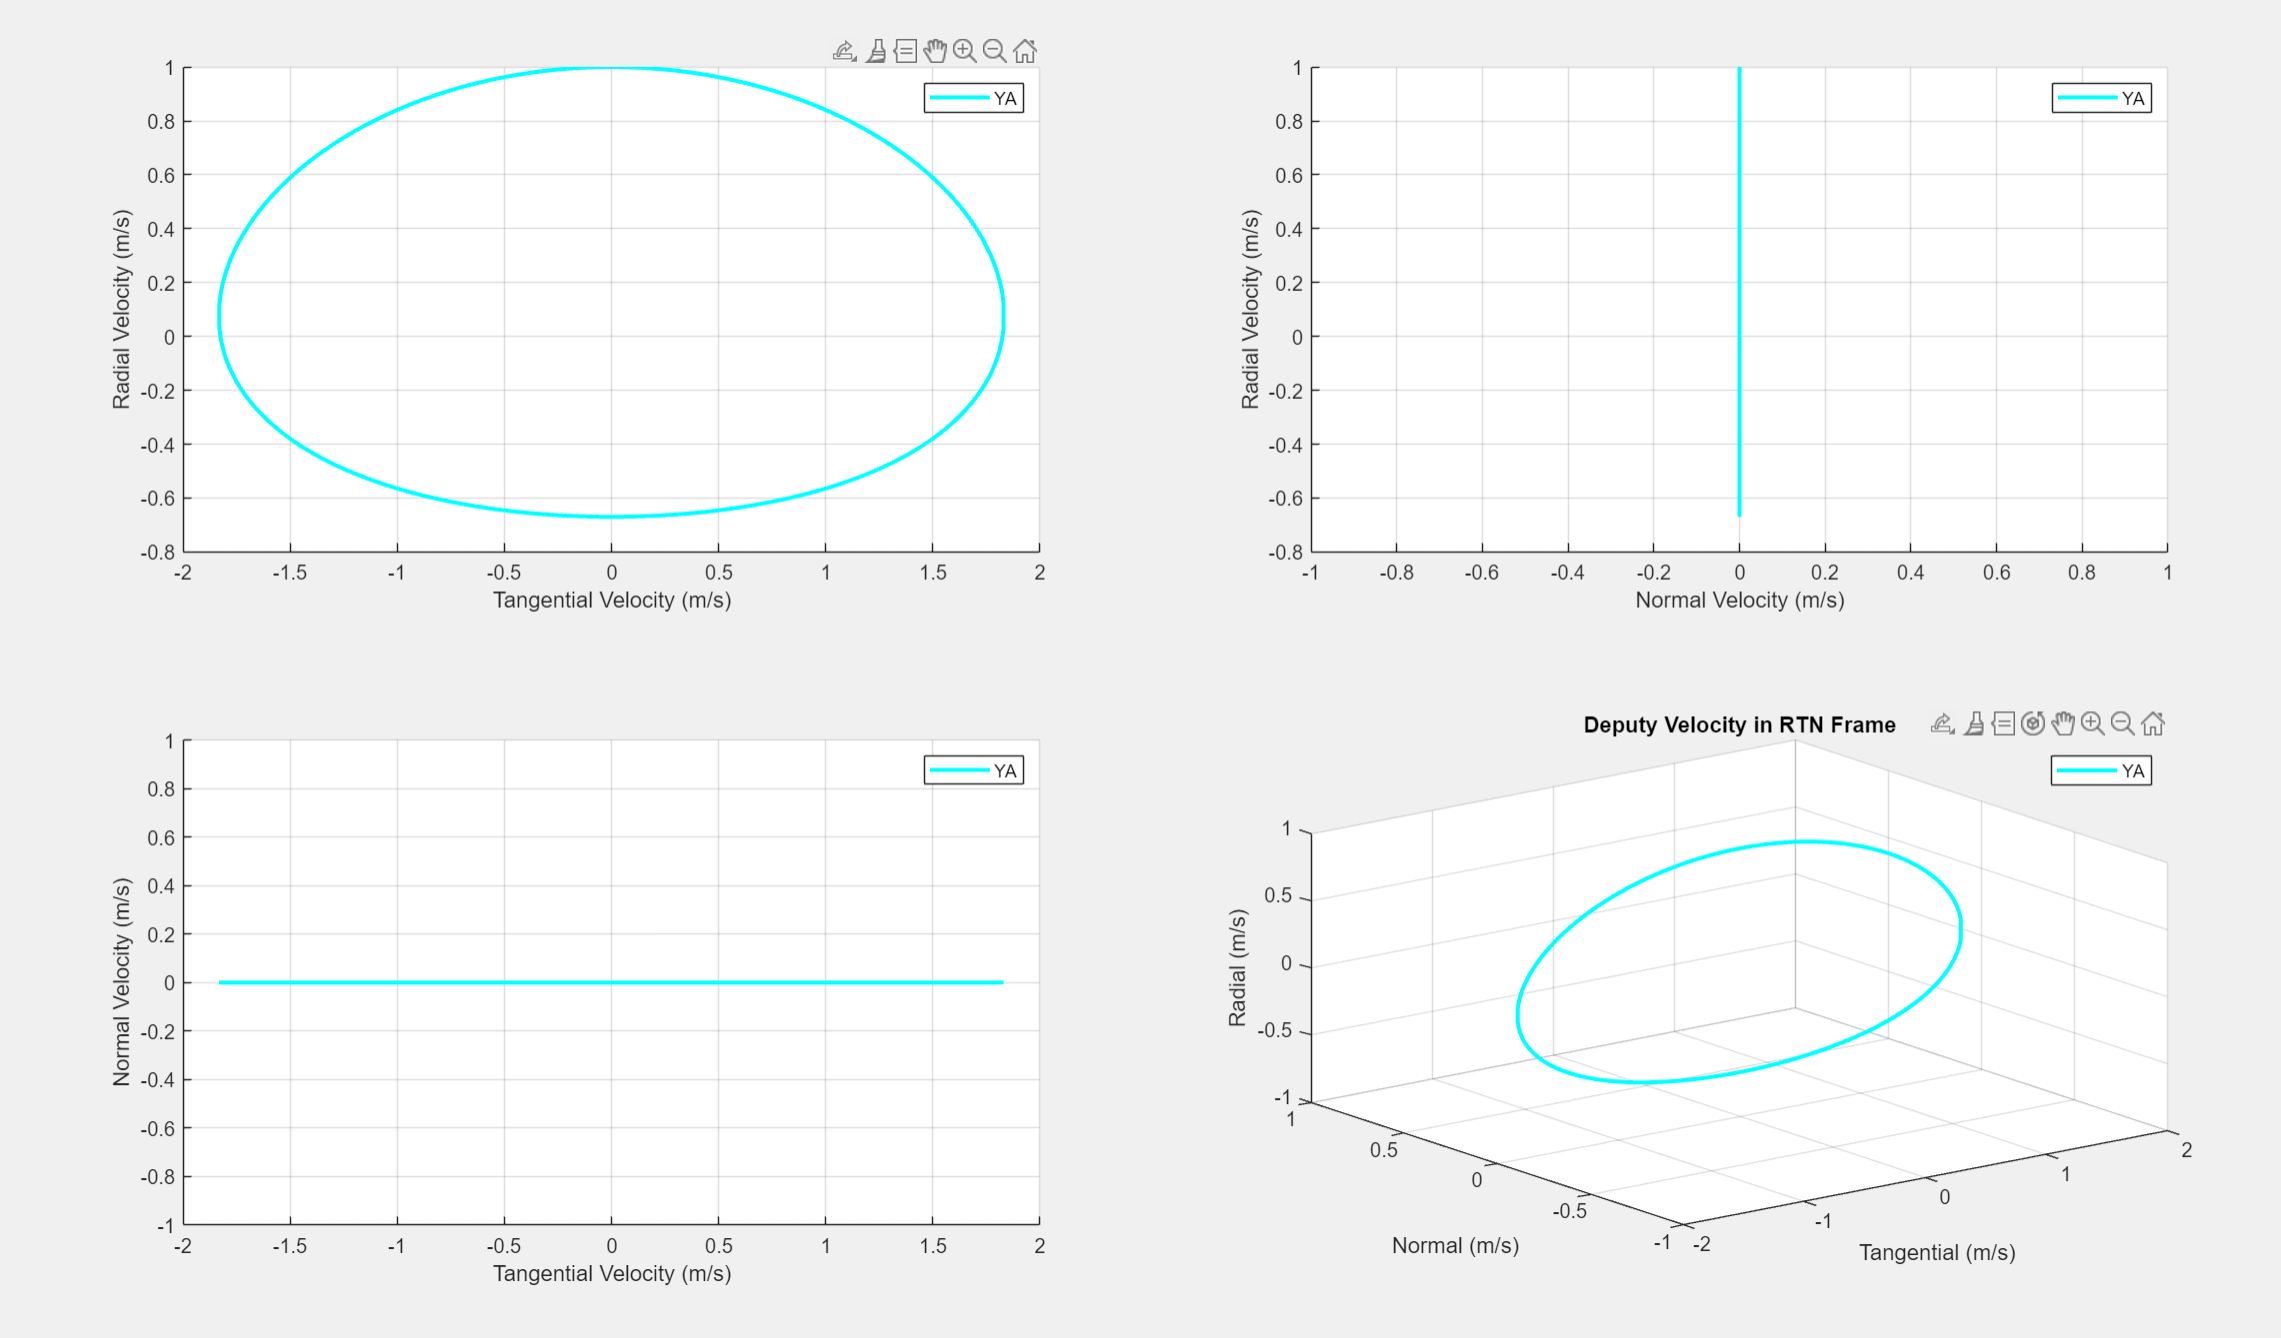
\includegraphics[width=0.7\textwidth]{PS3/Figures/YA_velocity.png}
    \caption{Deputy velocity in RTN frame from YA Equations}
    \label{fig:ya_velocity}
\end{figure}

\subsubsection{Expected Behavior}

The behavior we see in these plots aligns with expectations. Since the initial conditions involve a difference in the along track direction, with a radial velocity difference, there is no semi major axis difference, and therefore no energy difference, between the orbits. Thus, as expected, we see bounded relative motion with no drift.

\subsubsection{Propagation with ROE Geometric Mapping}
We propagate the relative motion using the geometric linear mapping with these relative orbit elements. This approach directly translates the ROE to relative position and velocity without solving differential equations.

\begin{figure}[H]
    \centering
    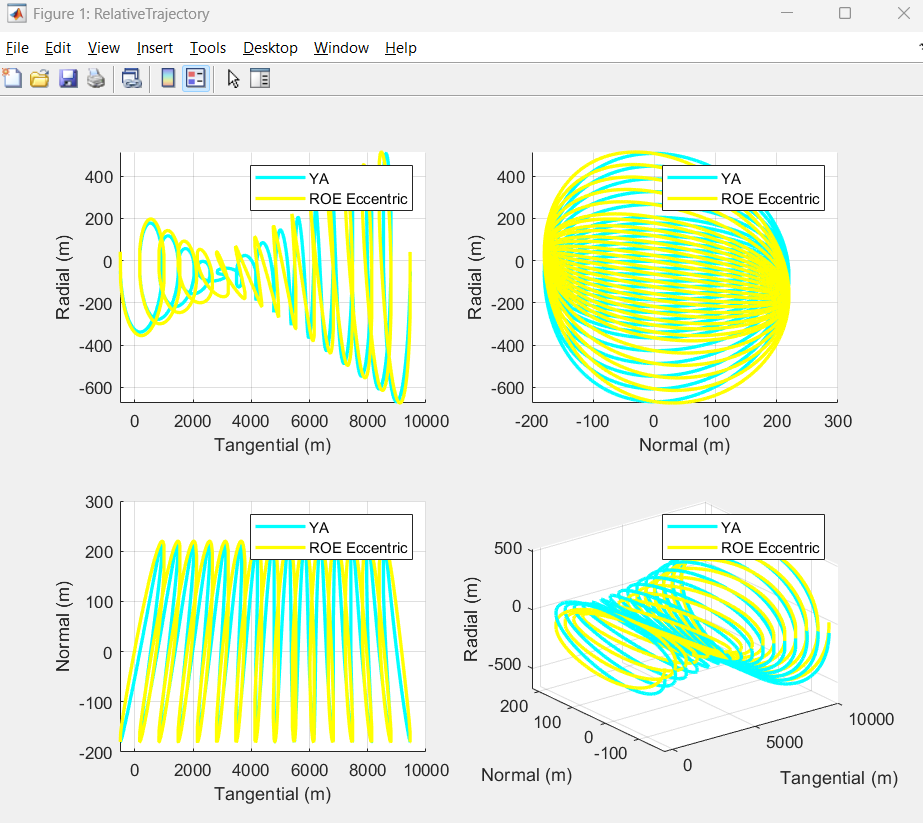
\includegraphics[width=0.7\textwidth]{PS3/Figures/ROE_YA_Position.png}
    \caption{Comparison of deputy trajectory from YA and ROE propagation in RTN frame}
    \label{fig:roe_ya_position}
\end{figure}

\begin{figure}[H]
    \centering
    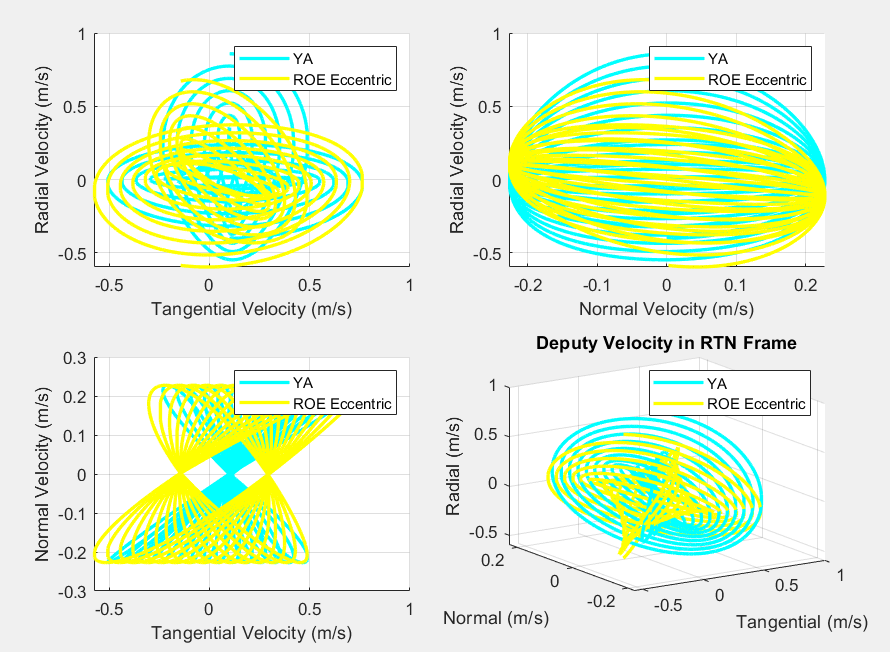
\includegraphics[width=0.7\textwidth]{PS3/Figures/ROE_YA_Velocity.png}
    \caption{Comparison of deputy velocity from YA and ROE propagation in RTN frame}
    \label{fig:roe_ya_velocity}
\end{figure}

\subsubsection{Analysis of Results}
The ROE propagation shows bounded motion as expected since δa = 0, which confirms the energy matching condition. While both YA and ROE solutions produce similar qualitative behavior, there are differences in amplitude and phase. 

The relationship between YA integration constants and ROE is mathematically consistent but not immediately obvious in the numerical values. Both represent the same physical motion using different parameterizations. The ROE approach offers a more intuitive physical interpretation, where each element corresponds directly to an aspect of relative motion.

\subsubsection{Comparison with Nonlinear Propagation}
To verify the accuracy of both solutions, we compare them with a nonlinear propagation that doesn't rely on linearization assumptions.

%\begin{figure}[H]
%    \centering
%    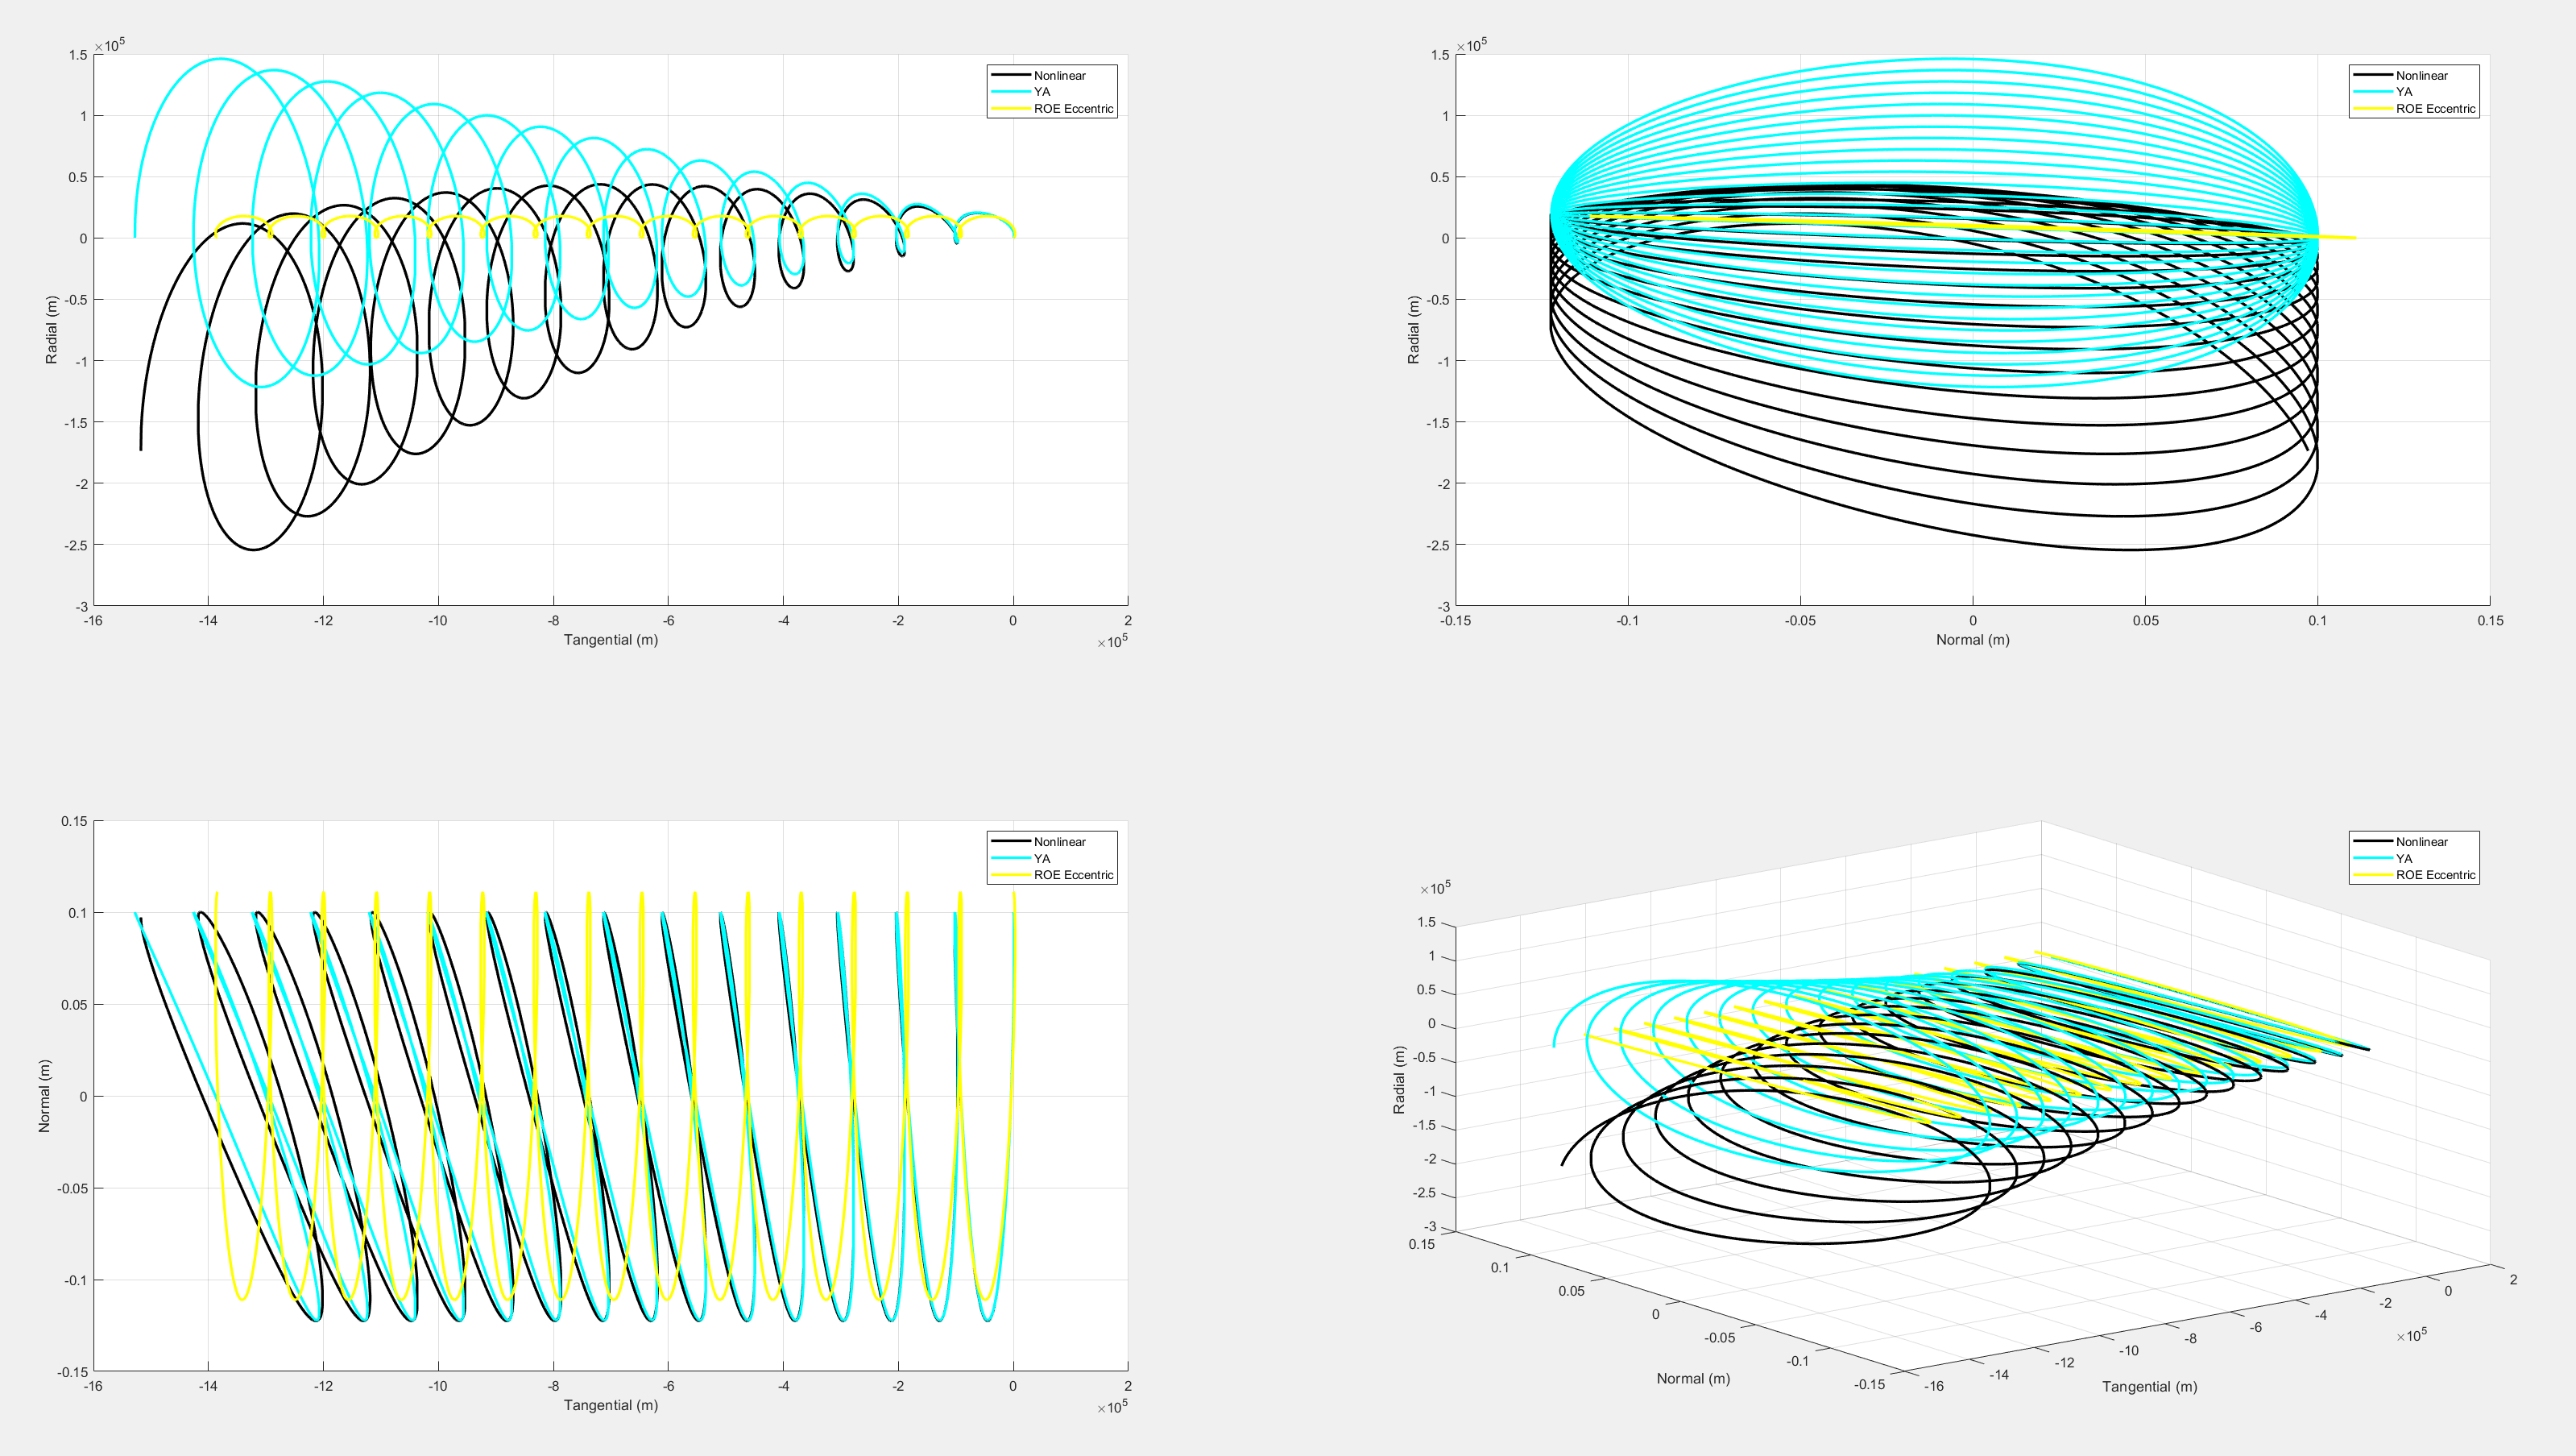
\includegraphics[width=0.7\textwidth]{PS3/Figures/Nonlinear_Position_Comparison.png}
%    \caption{Comparison of deputy trajectory with nonlinear propagation}
%    \label{fig:nonlinear_position_comparison}
%\end{figure}

%\begin{figure}[H]
%    \centering
%    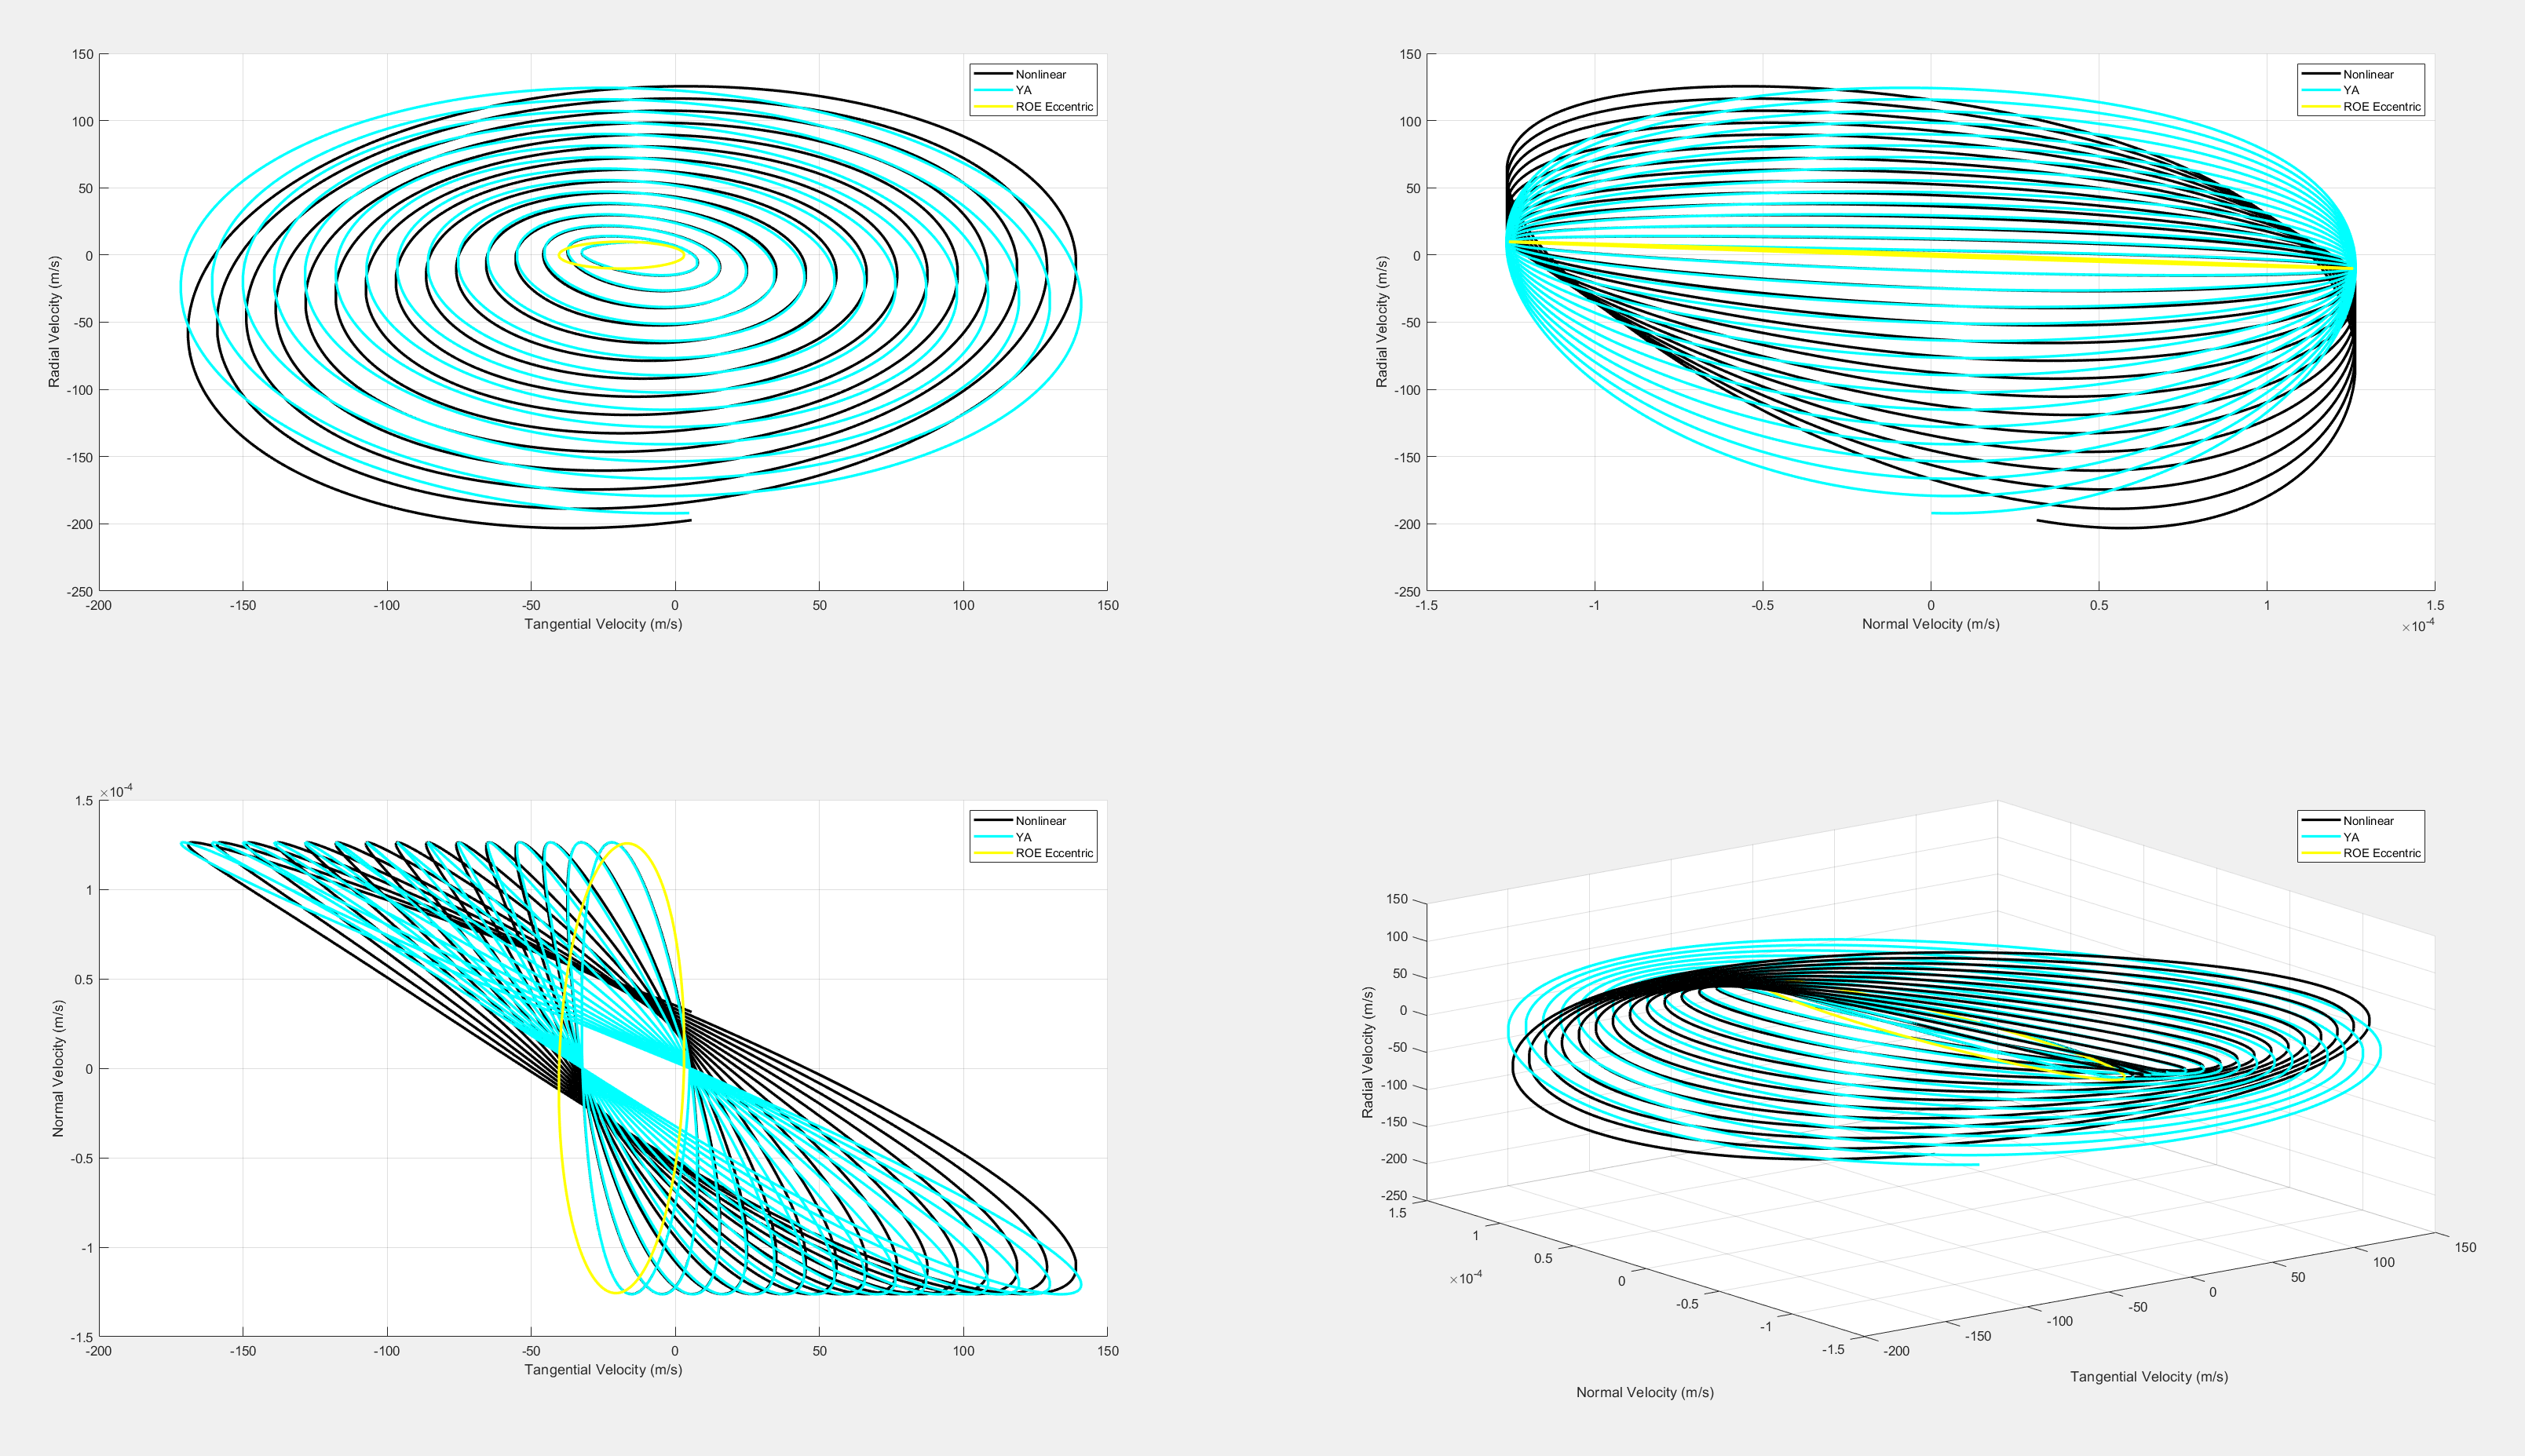
\includegraphics[width=0.7\textwidth]{PS3/Figures/Nonlinear_Velocity_Comparison.png}
%    \caption{Comparison of deputy velocity with nonlinear propagation}
%    \label{fig:nonlinear_velocity_comparison}
%\end{figure}

%\begin{figure}[H]
%    \centering
%    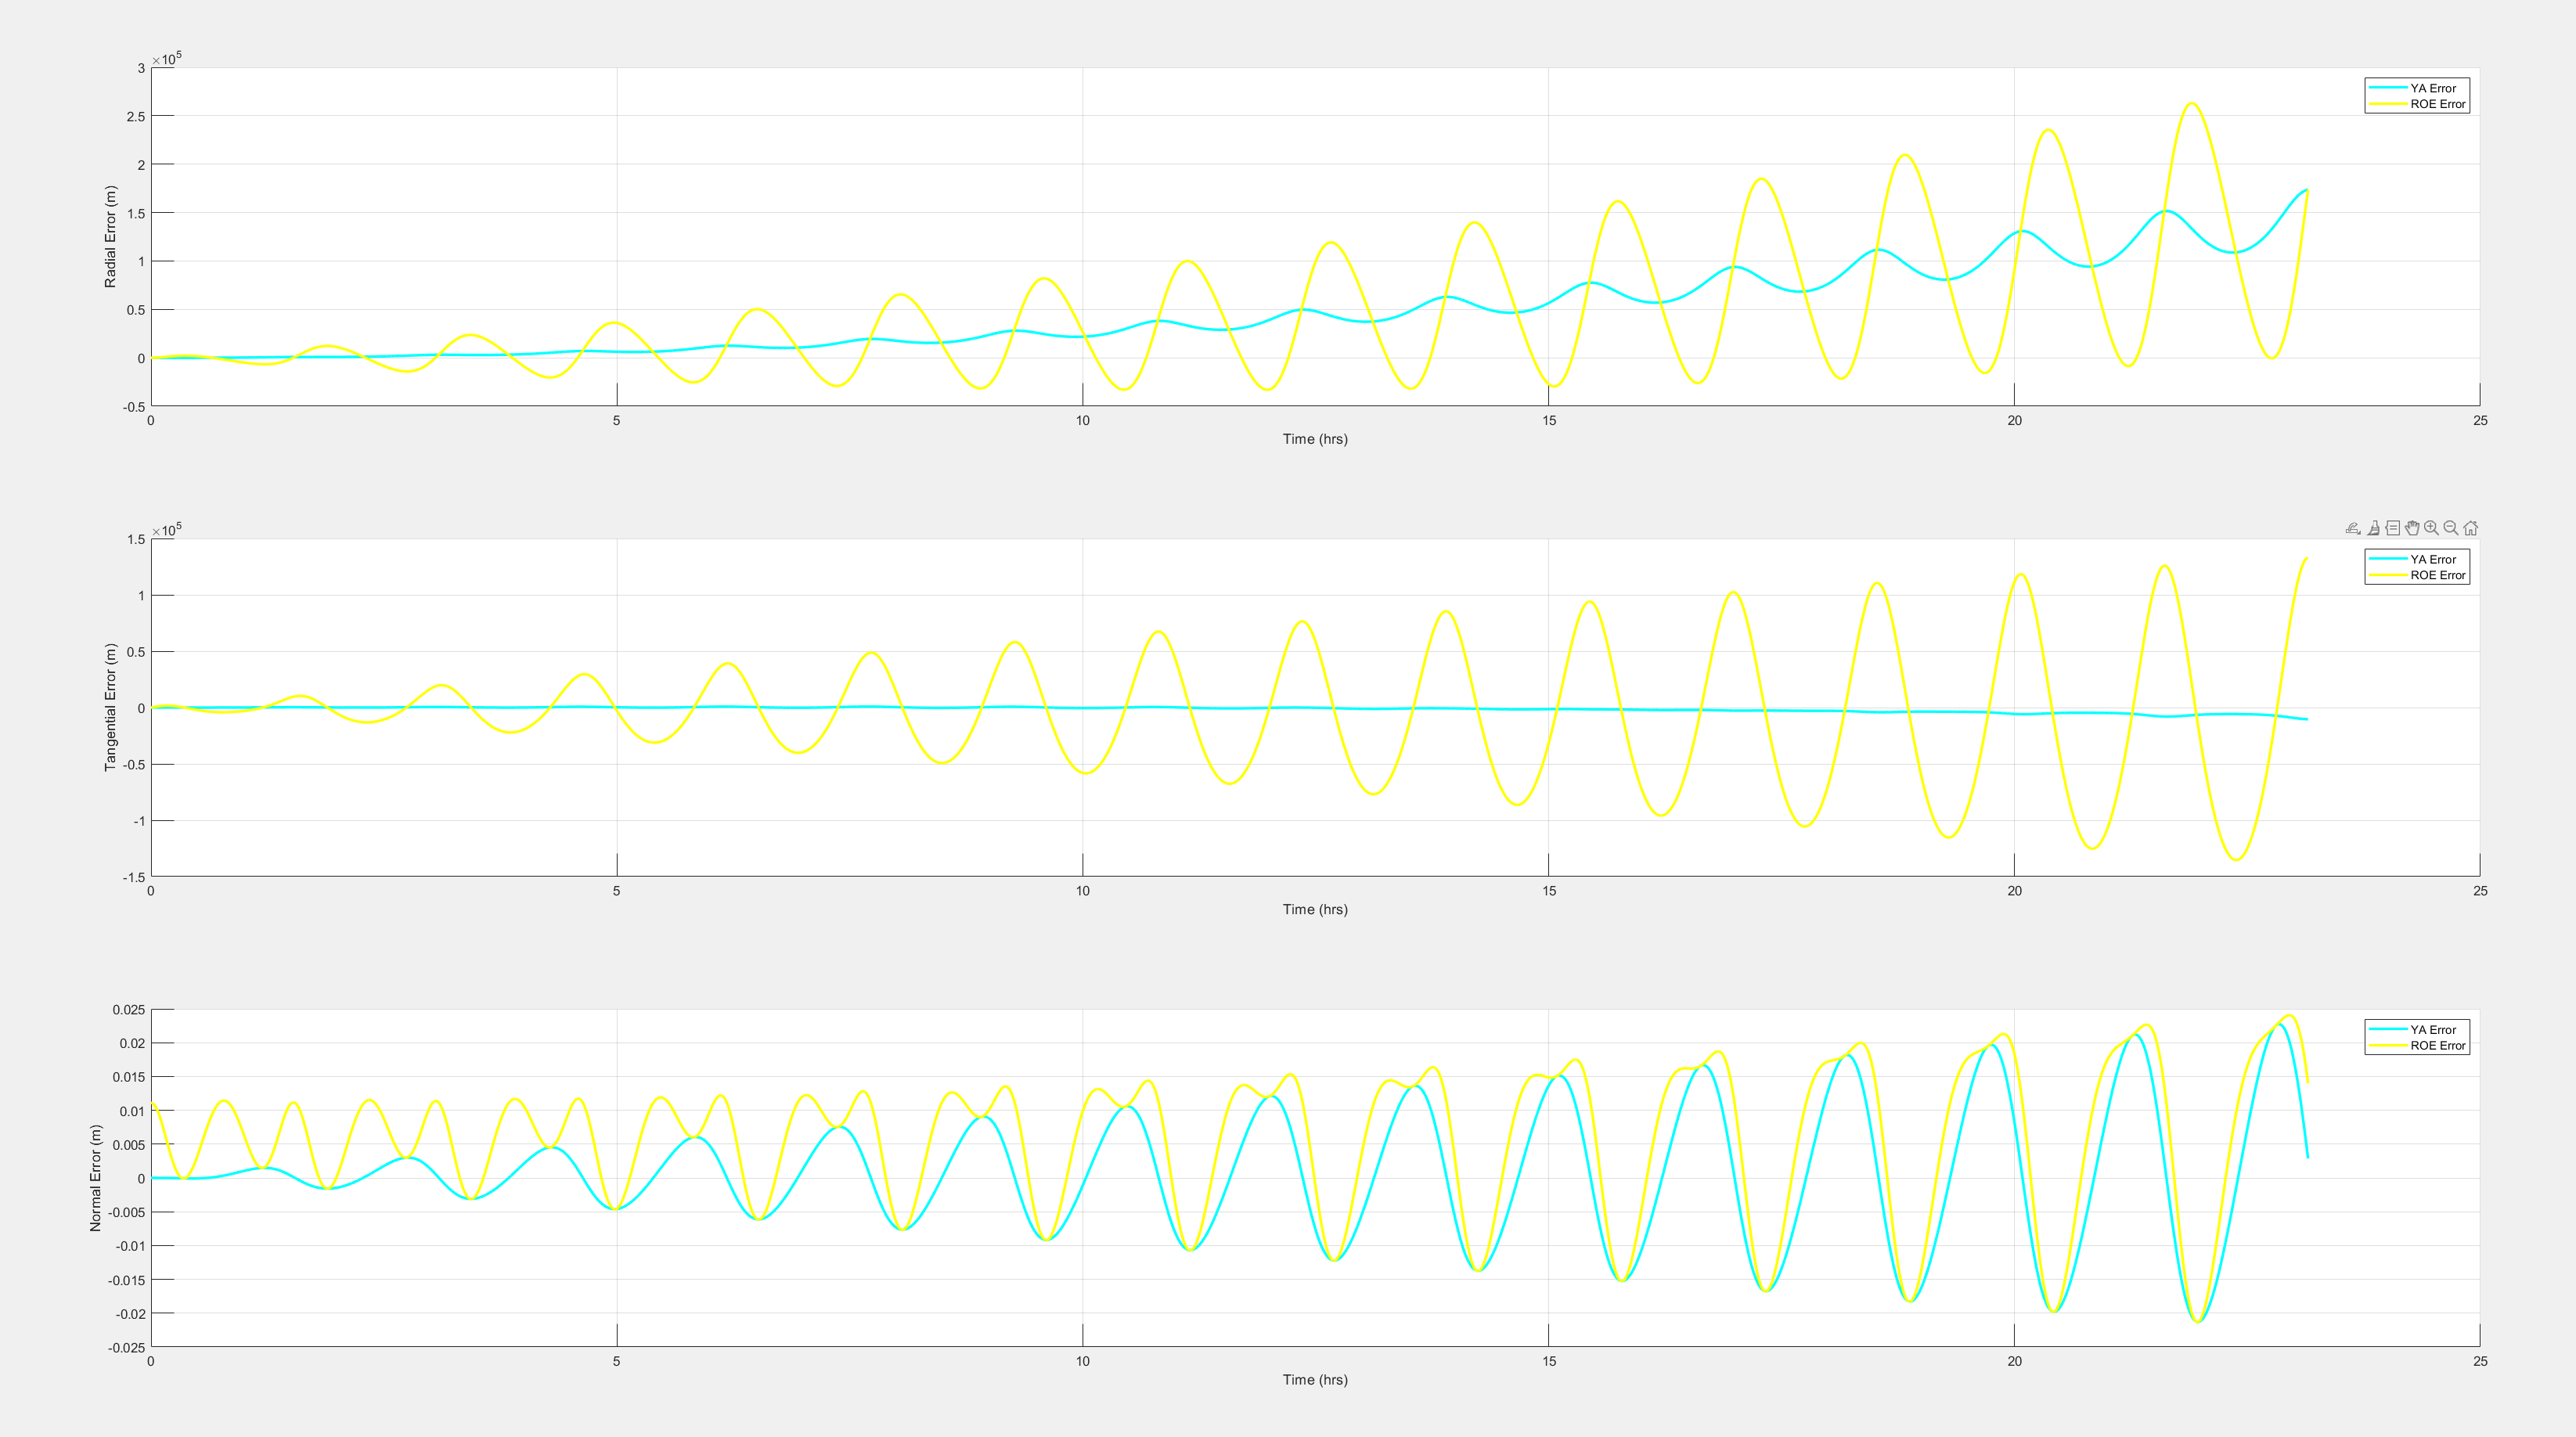
\includegraphics[width=0.7\textwidth]{PS3/Figures/Position_Error_Analysis.png}
%    \caption{Position propagation errors in RTN frame}
%    \label{fig:position_error_analysis}
%\end{figure}

%\begin{figure}[H]
%    \centering
%    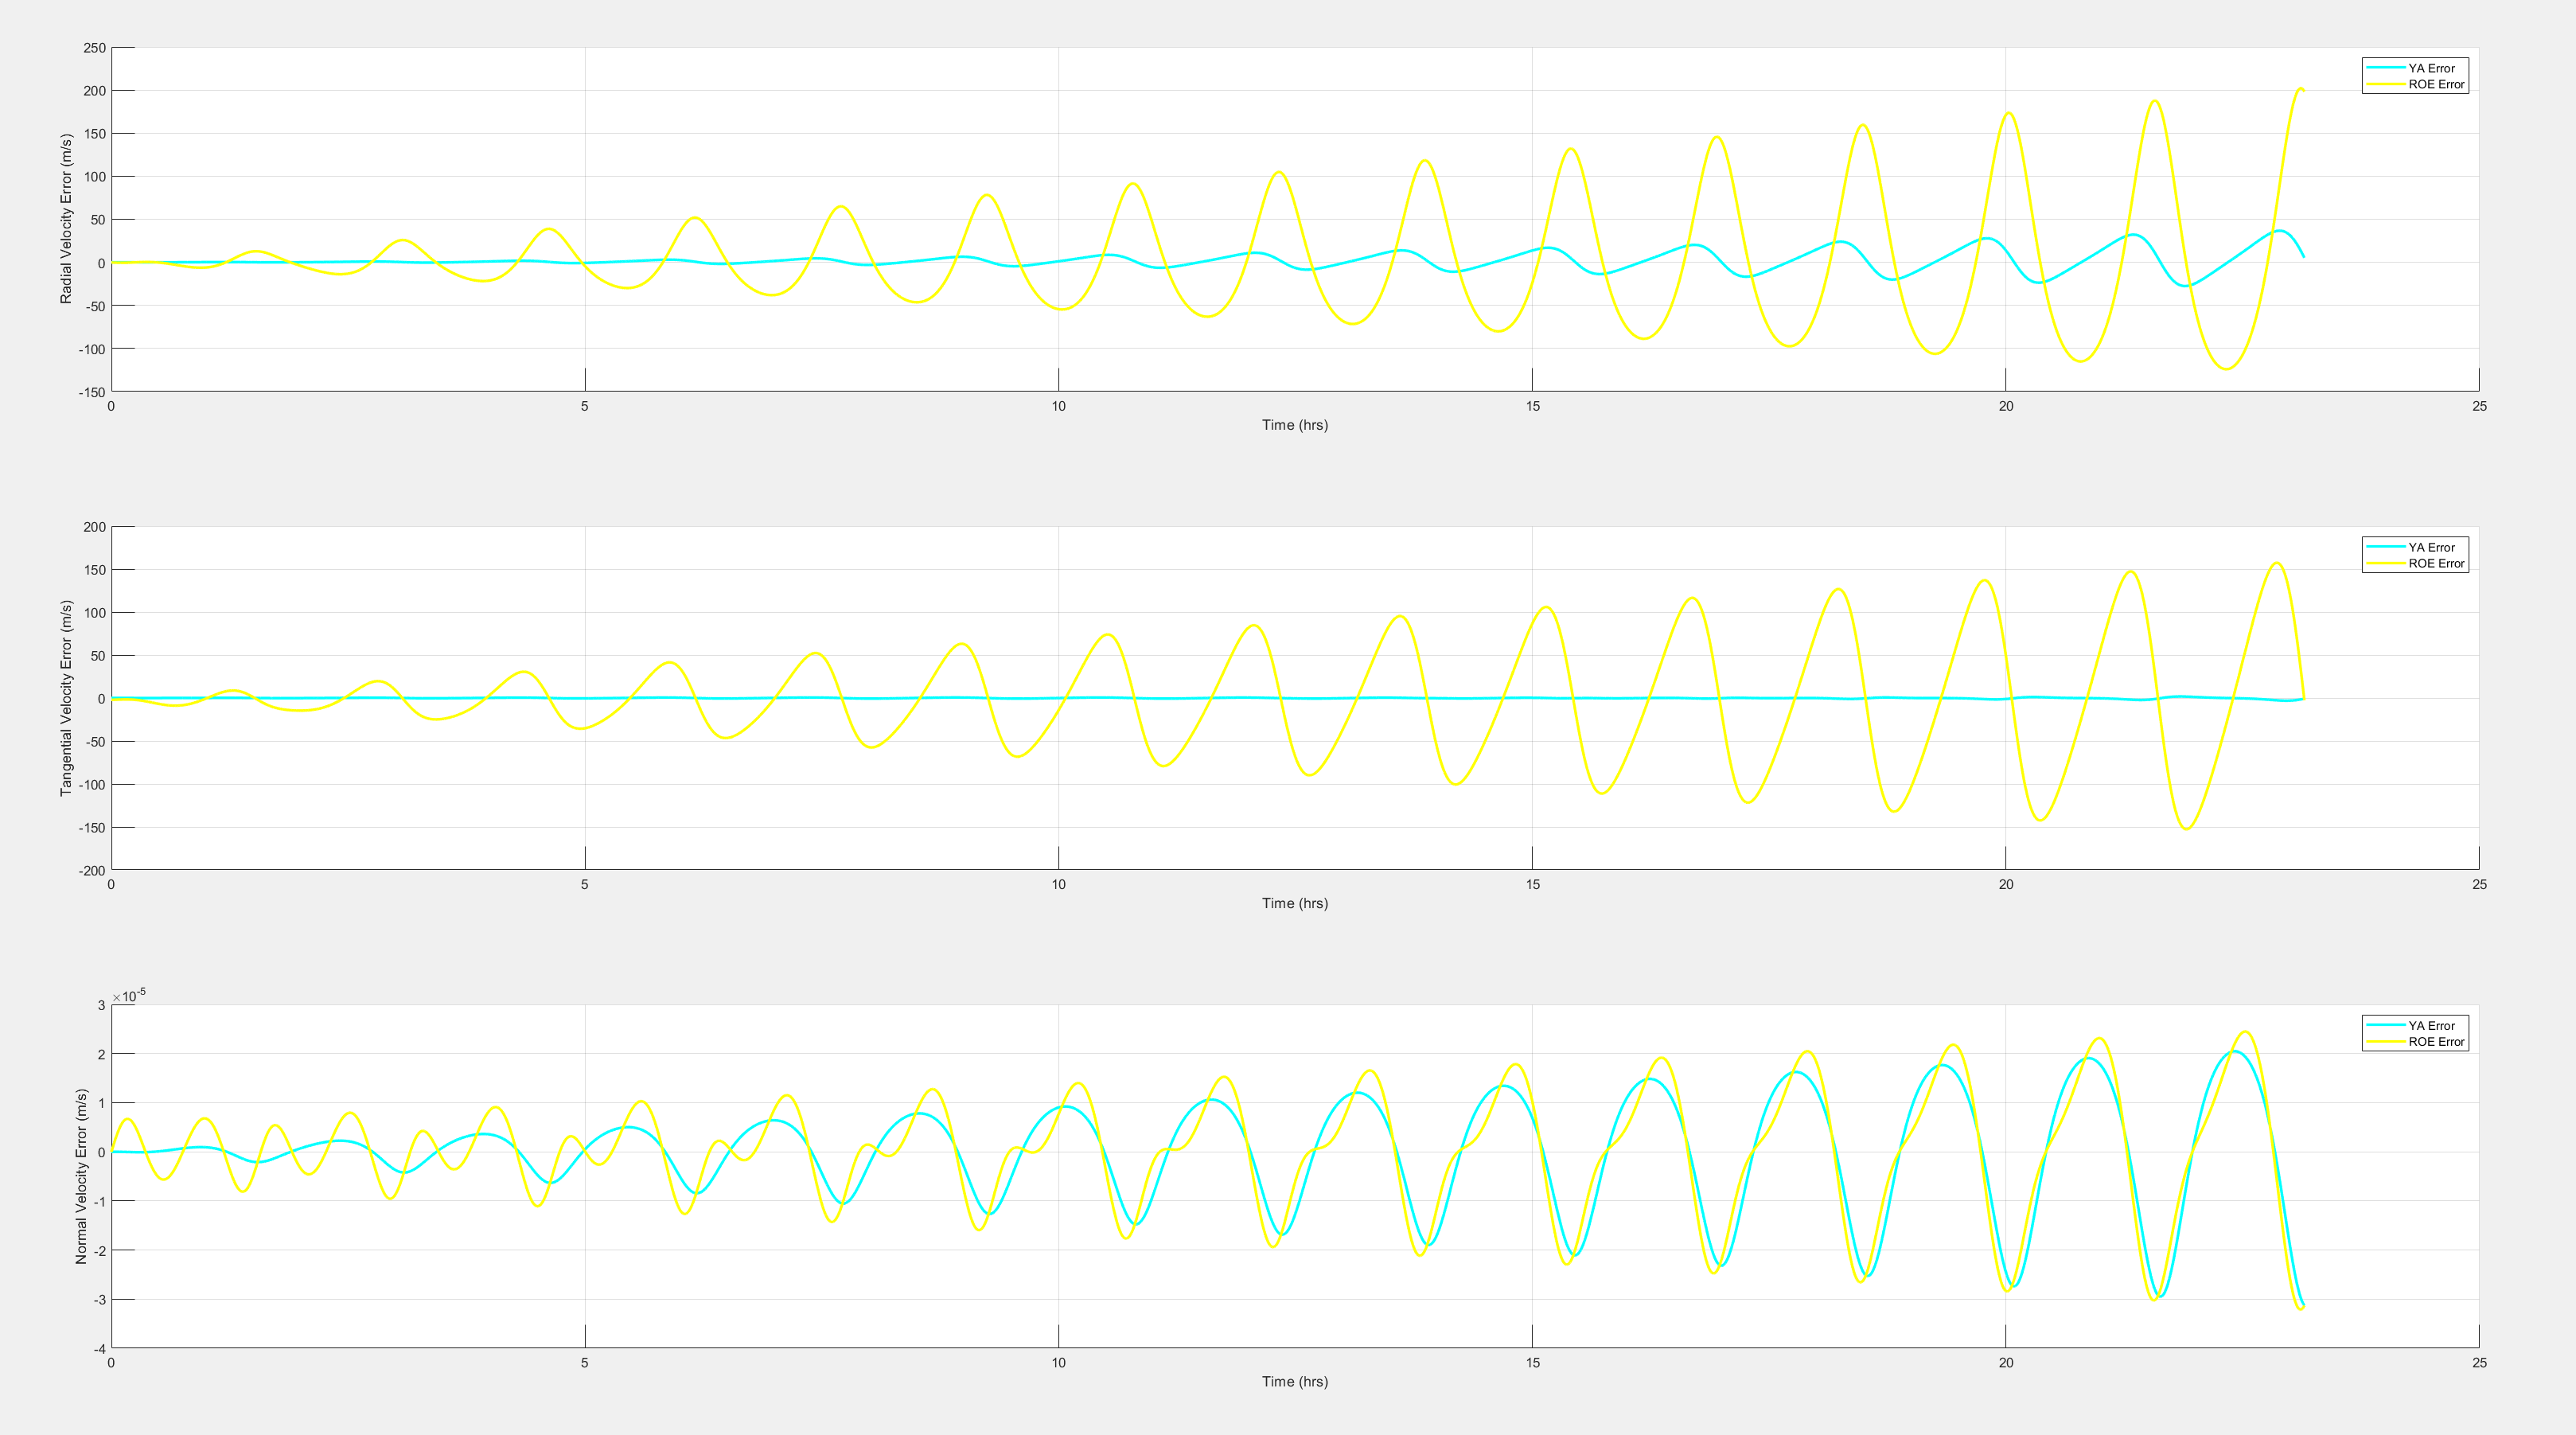
\includegraphics[width=0.7\textwidth]{PS3/Figures/Velocity_Error_Analysis.png}
%    \caption{Velocity propagation errors in RTN frame}
%    \label{fig:velocity_error_analysis}
%\end{figure}

For our scenario with e=0.1, the YA solution provides slightly better accuracy than the ROE geometric mapping implementation. The YA solution directly integrates the linearized differential equations, which can capture more dynamic effects than the static geometric mapping used in our ROE implementation. However, both methods show good qualitative agreement with the nonlinear solution.

\subsubsection{Case Study: Semi-Major Axis Difference}
We now modify our initial conditions to include a radial offset of 10 meters, creating a small difference in semi-major axis. This value is small enough to remain within linearization assumptions but large enough to produce visible drift over 15 orbits.

%\begin{figure}[H]
%    \centering
%    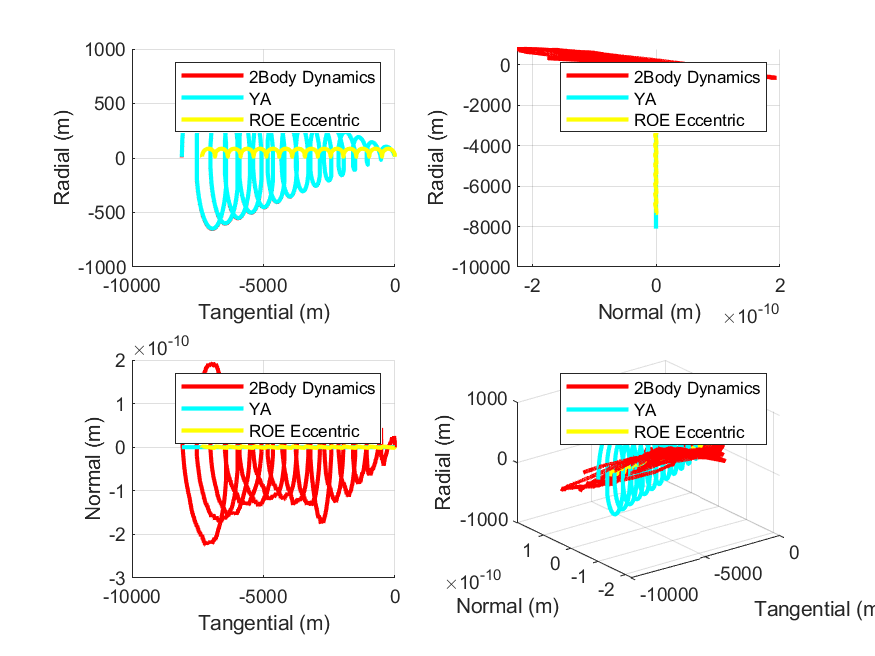
\includegraphics[width=0.7\textwidth]{PS3/Figures/SMA_Difference_Position.png}
%    \caption{Deputy trajectory with semi-major axis difference}
%    \label{fig:sma_difference_position}
%\end{figure}

%\begin{figure}[H]
%    \centering
%    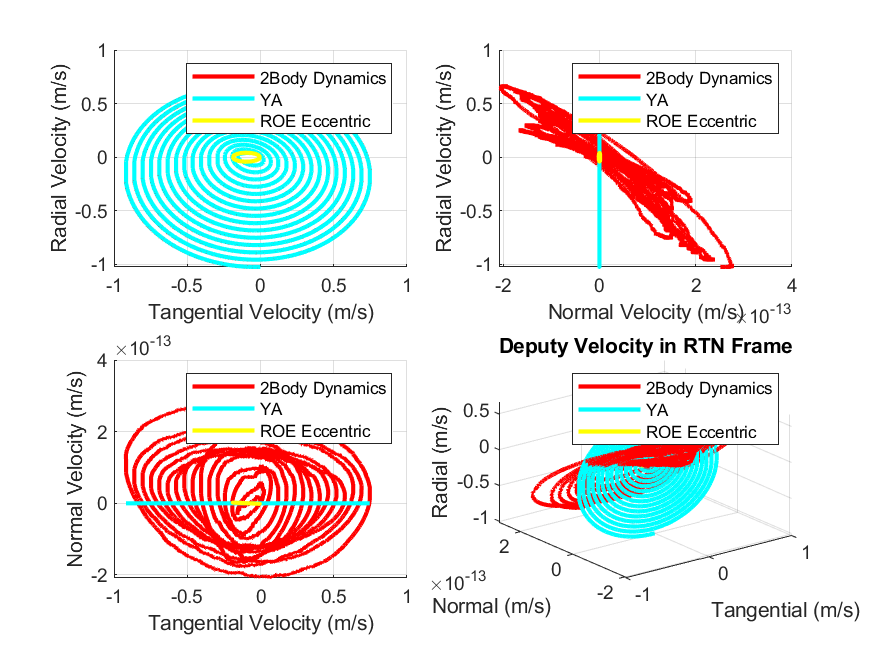
\includegraphics[width=0.7\textwidth]{PS3/Figures/SMA_Difference_Velocity.png}
%    \caption{Deputy velocity with semi-major axis difference}
%    \label{fig:sma_difference_velocity}
%\end{figure}

As expected, the results show secular drift in the along-track direction due to the different orbital periods. Both analytical solutions correctly capture this drift, which increases approximately linearly with time. The drift rate matches the theoretical prediction.

\subsubsection{Case Study: Highly Eccentric Orbit}
Finally, we analyze a case with high eccentricity (e=0.6) to test the limits of our linearized models.

%\begin{figure}[H]
%    \centering
%    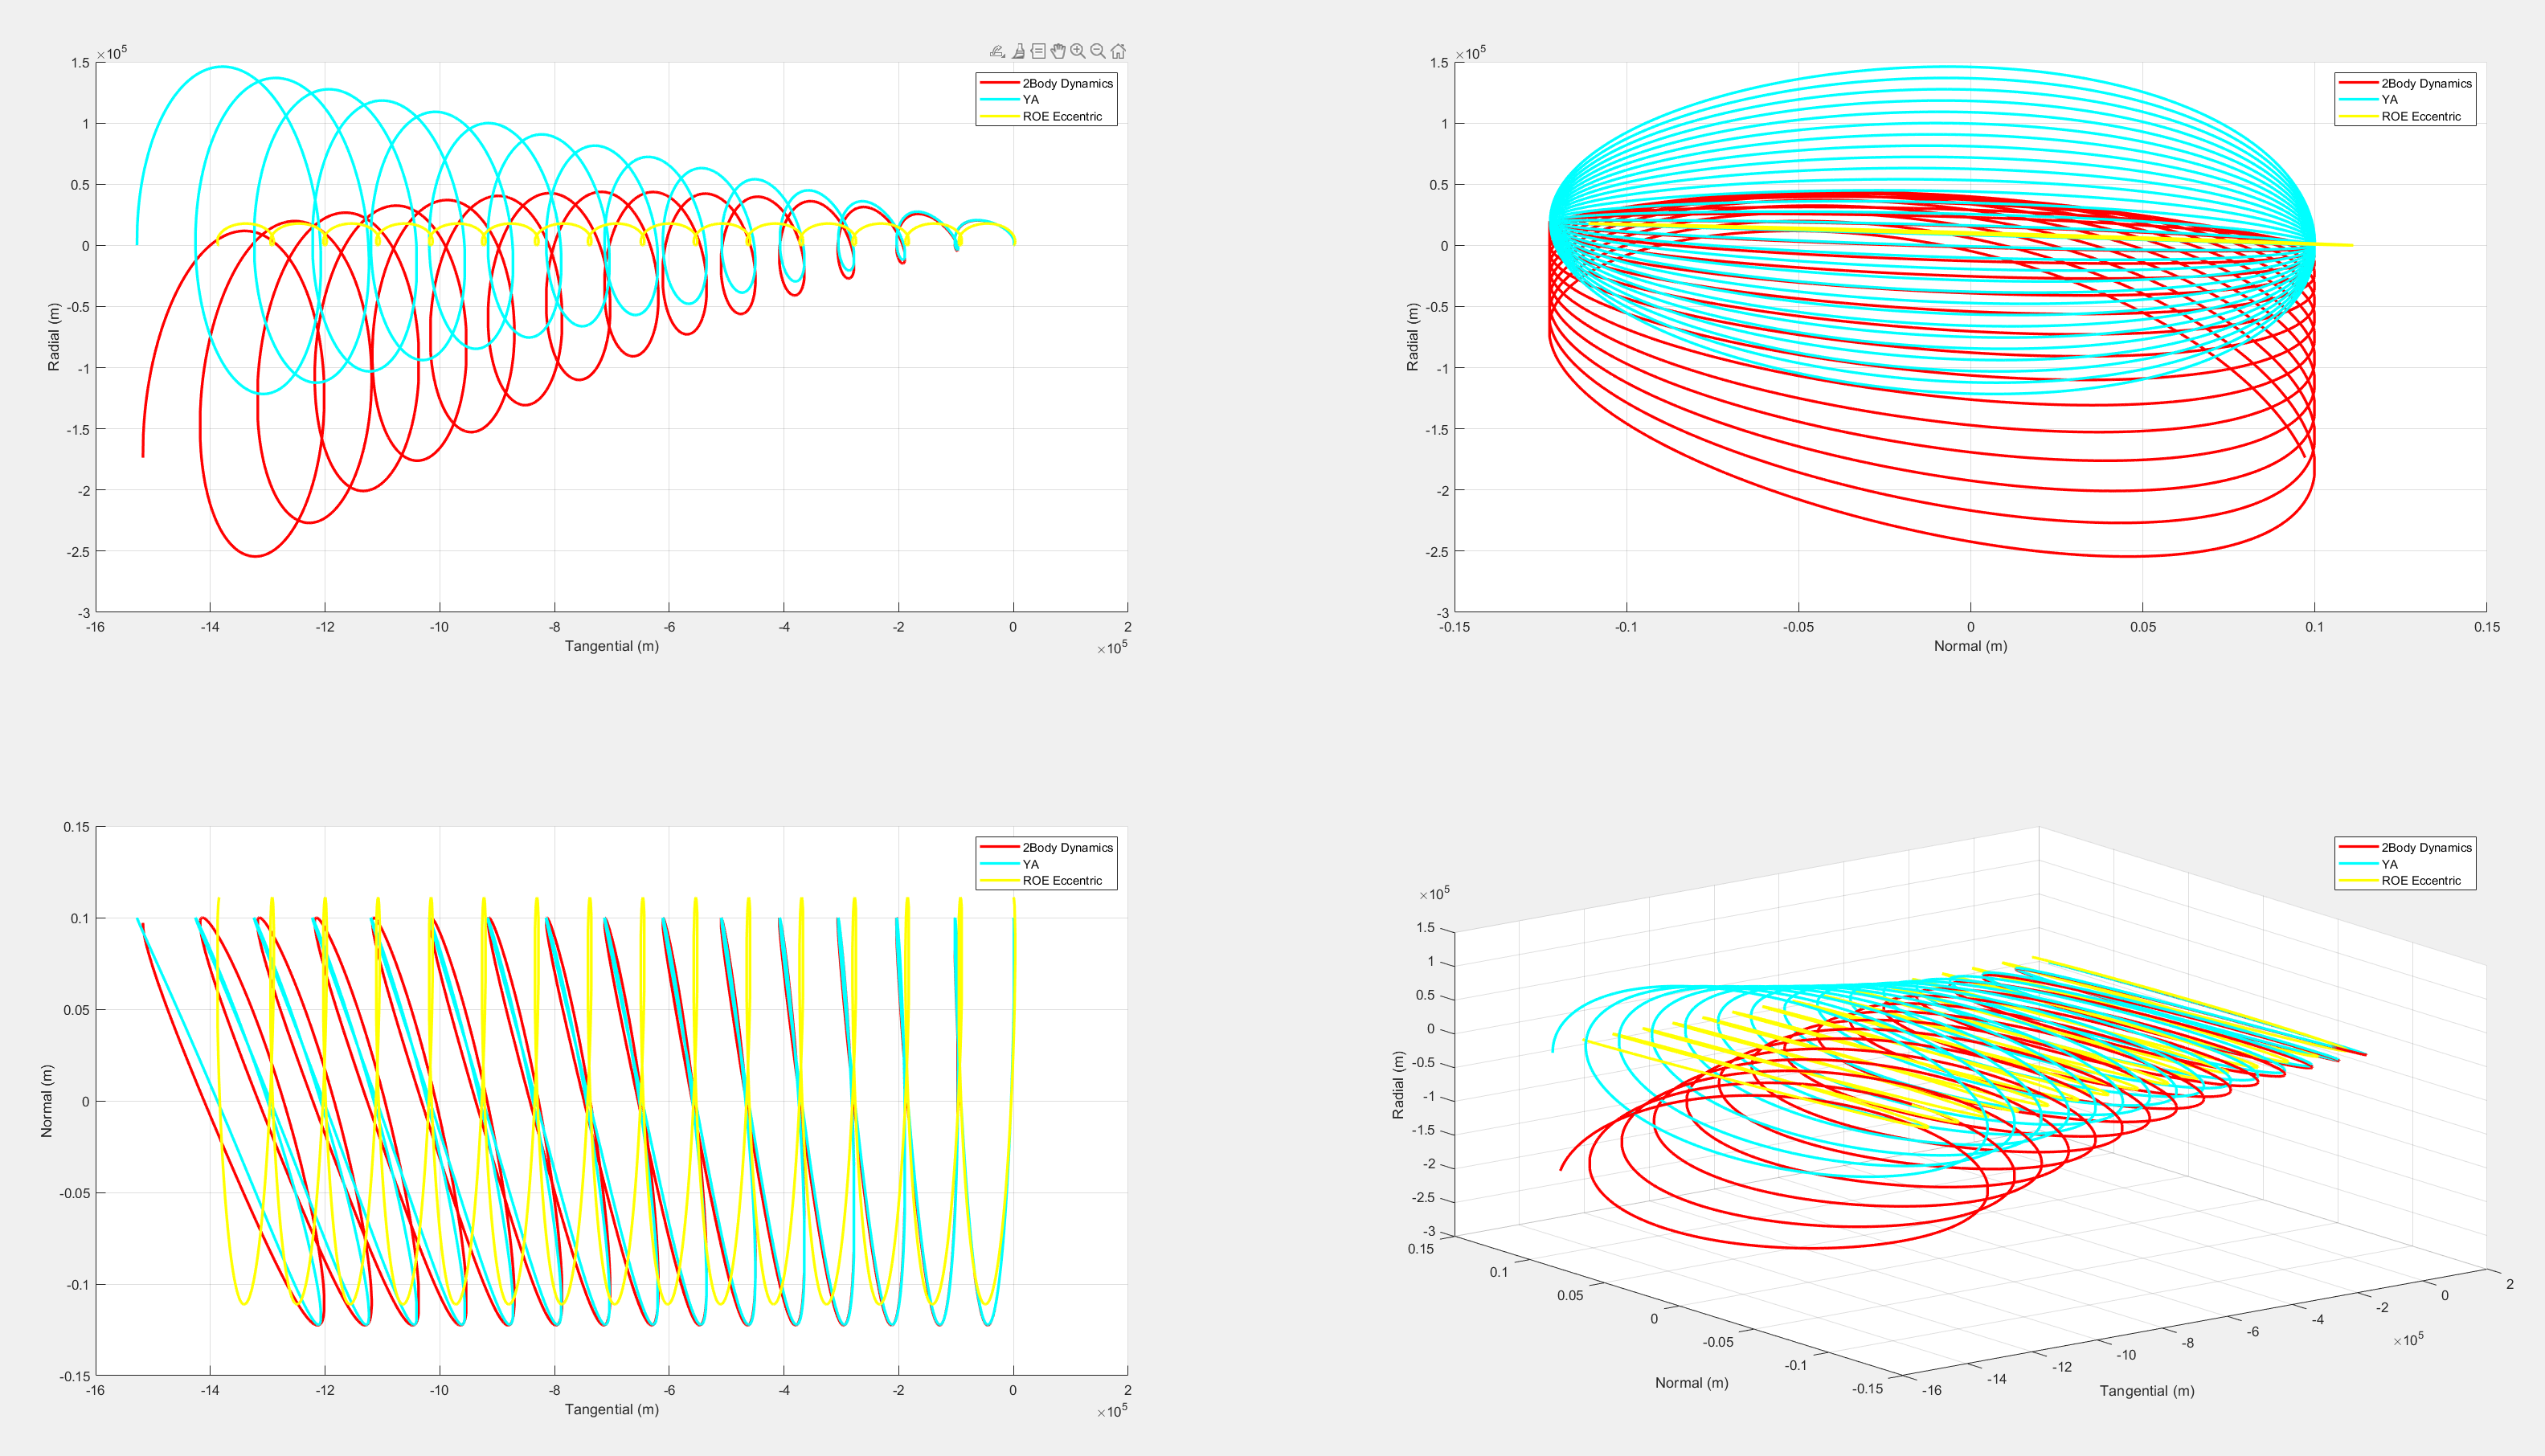
\includegraphics[width=0.7\textwidth]{PS3/Figures/High_Eccentricity_Position.png}
%    \caption{Deputy trajectory with highly eccentric orbit (e=0.6)}
%    \label{fig:high_eccentricity_position}
%\end{figure}

%\begin{figure}[H]
%    \centering
%    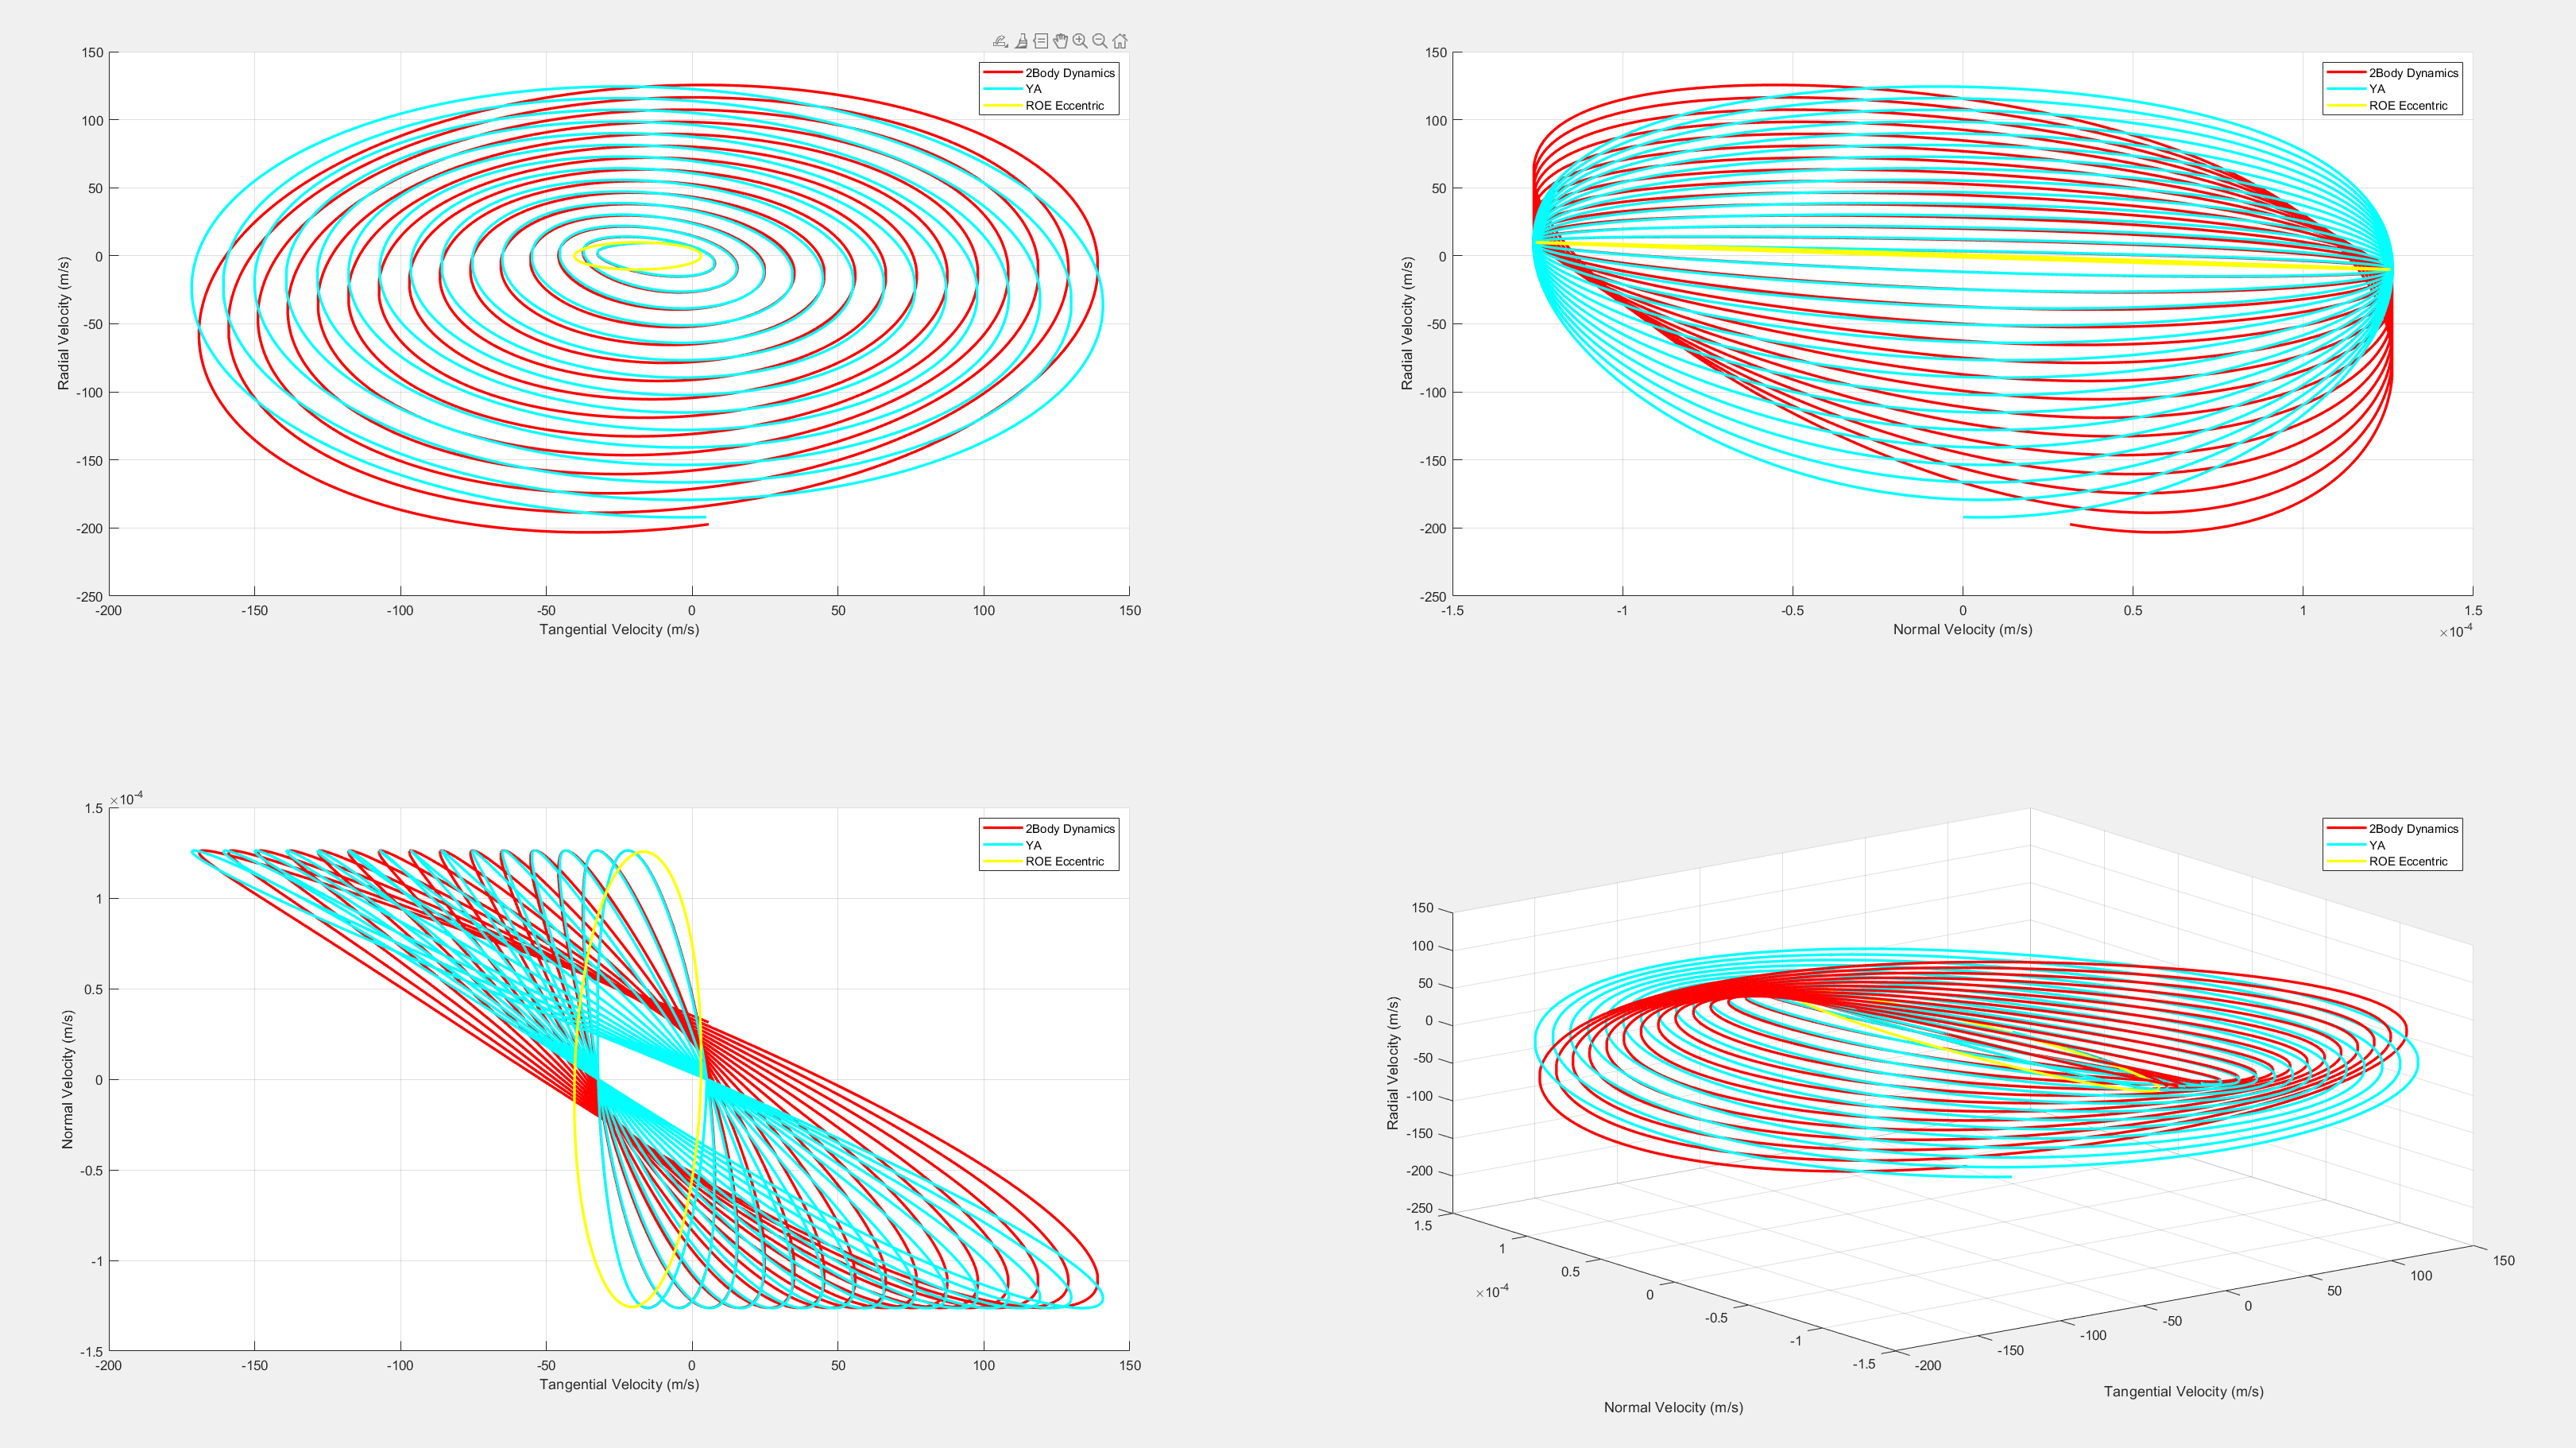
\includegraphics[width=0.7\textwidth]{PS3/Figures/High_Eccentricity_Velocity.png}
%    \caption{Deputy velocity with highly eccentric orbit (e=0.6)}
%    \label{fig:high_eccentricity_velocity}
%\end{figure}

At this high eccentricity, we observe significant deviations between the linearized solutions and the nonlinear truth. The relative motion shows strong distortions near perigee passages, where orbital velocity changes rapidly. This demonstrates the limitations of linearized theories for highly eccentric orbits, as the linearization assumptions break down when eccentricity increases. For such cases, higher-order models or fully nonlinear methods would be required for accurate prediction of relative motion.

\newpage
\section{Problem Set 4}

\subsection{These are Relative Orbits}

\subsubsection{Initial Conditions}
For the first part of this problem, we set the initial conditions in classical orbital elements to be [6780000, 0.001, 0, 0, 0, 0]. This provides us with an eccentric orbit that is sufficiently far from the attractor's center. We then set the deputy's rtn coordinates to be [-50; -500; -180; -0.4; 0.1; 0], as we did in the last pset.

As requested for the second part, we keep the same initial orbit, but we set the osculating quasi non singular orbital elements to be [0, 100, 50, 100, 30, 200].

\subsubsection{Orbital Elements, Relative Orbital Elements}
First part, without J2:
\begin{figure}[H]
    \centering
    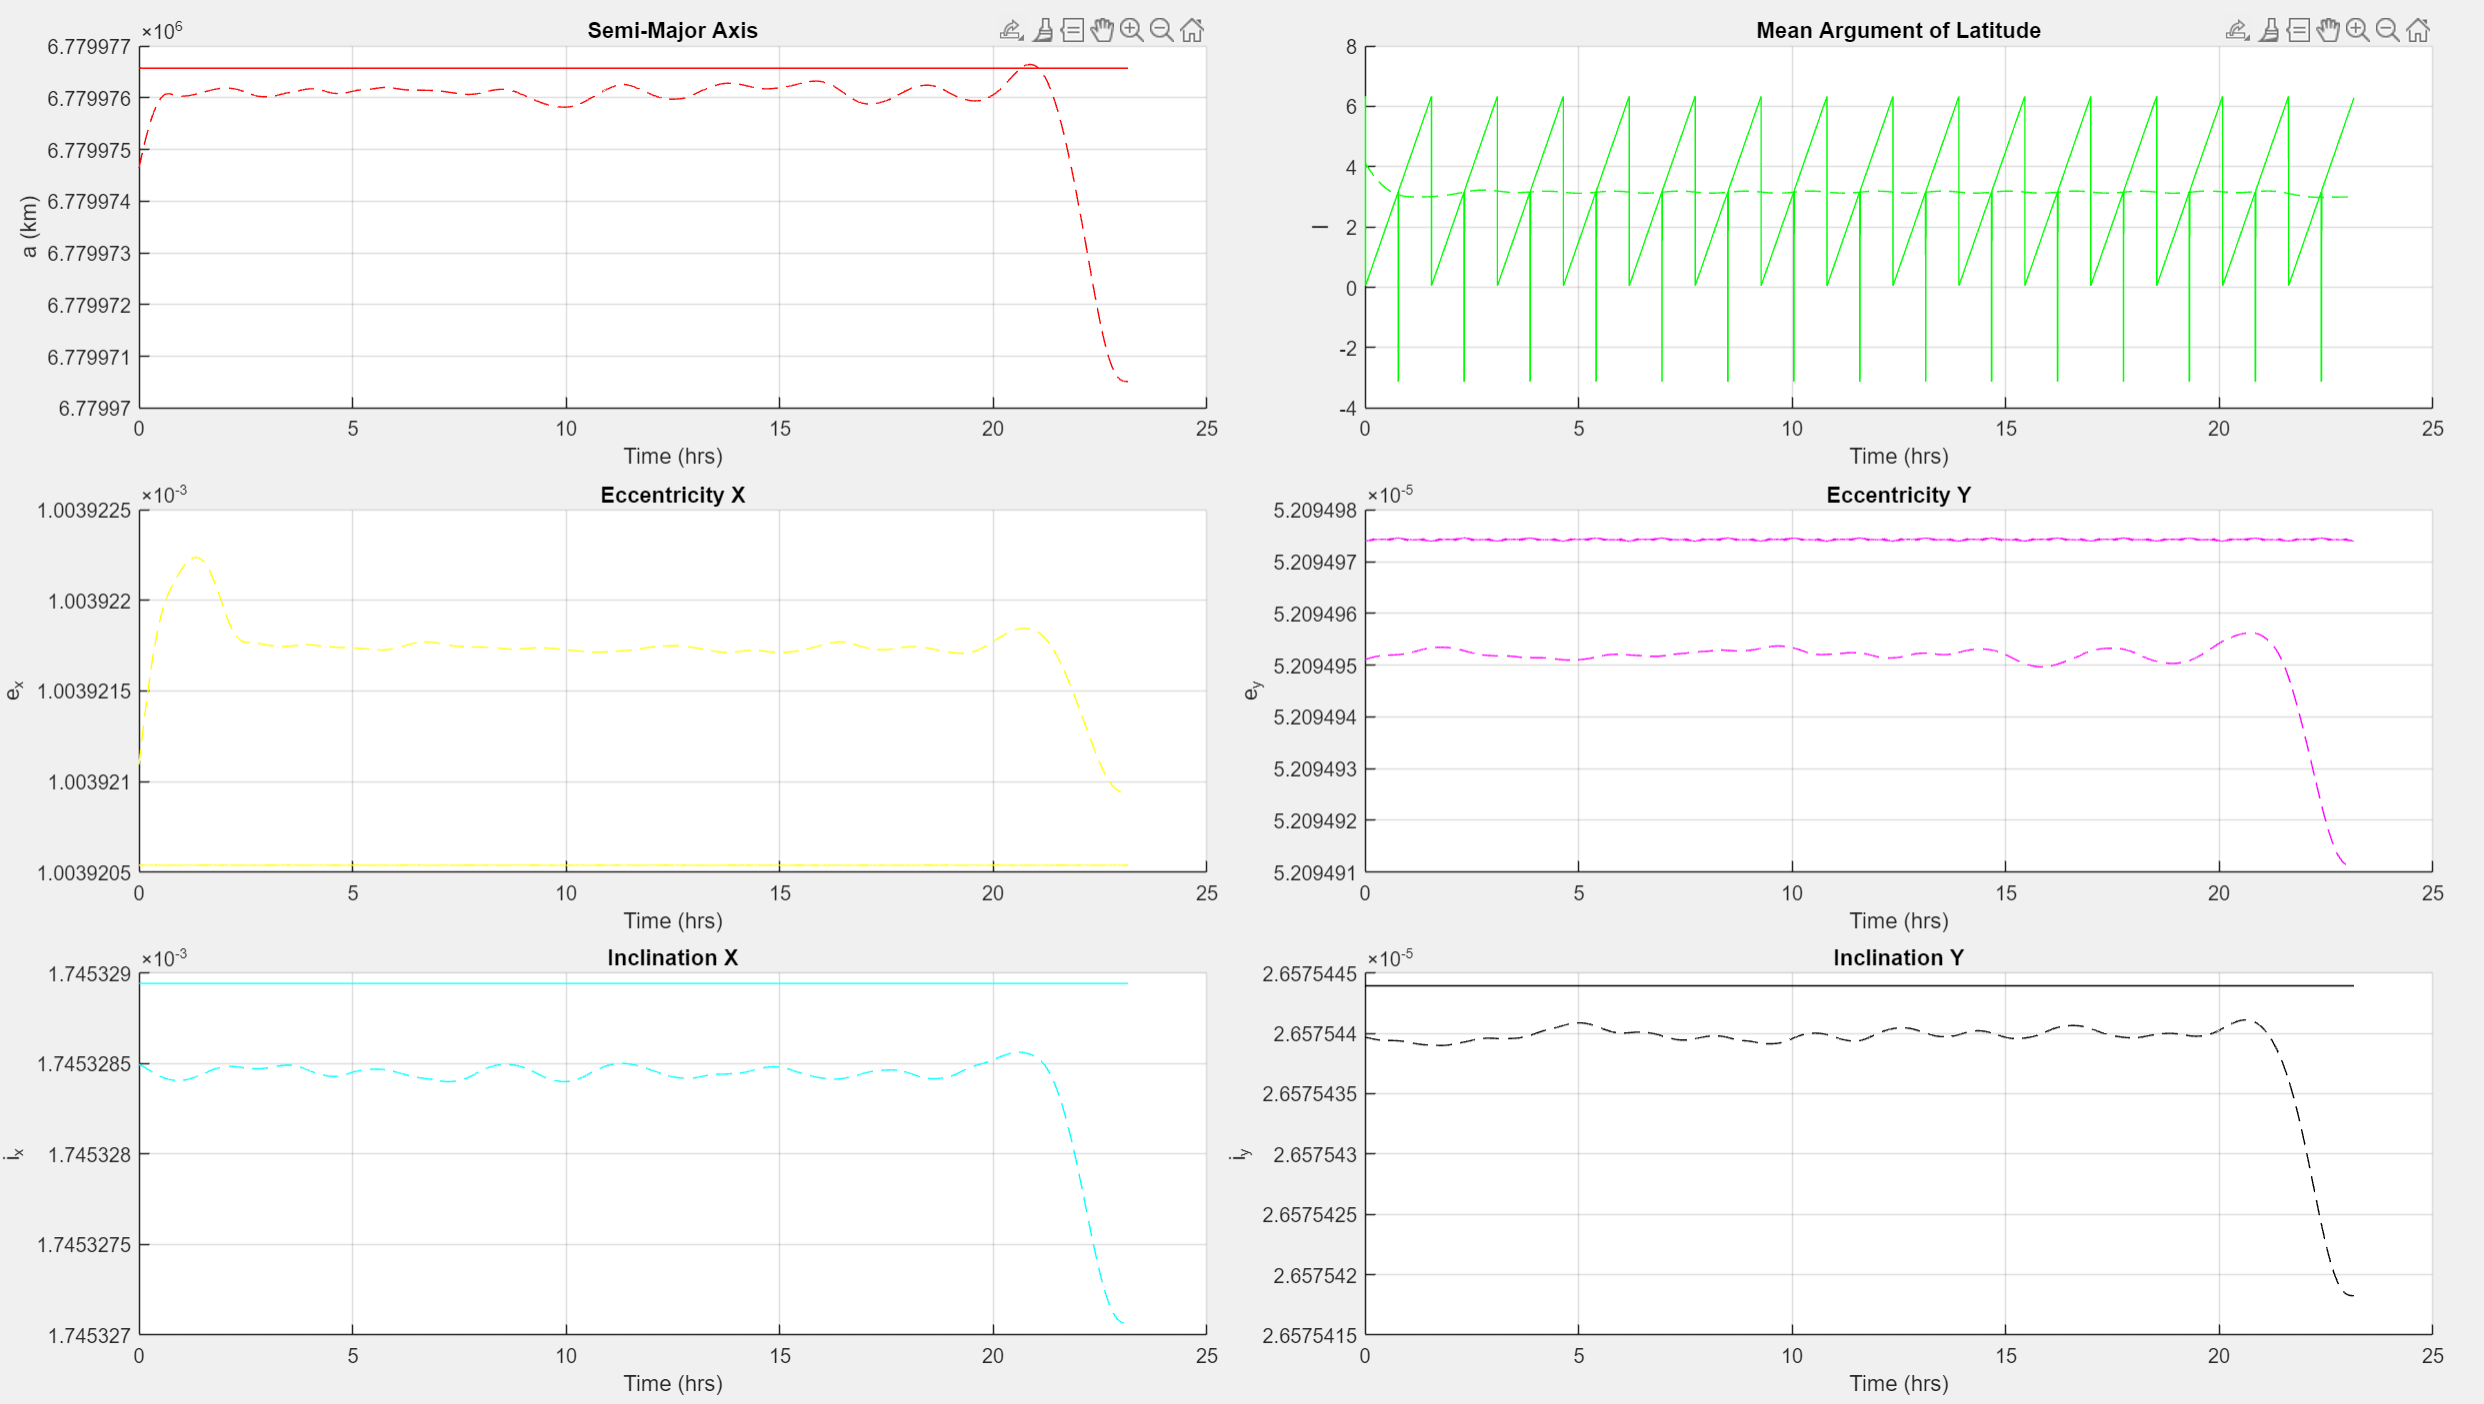
\includegraphics[width=0.7\textwidth]{PS4/Figures/case1_noJ2.png}
    \caption{Initial Conditions 1, Without J2, Quasi Nonsingular Orbital Elements}
    \label{fig:hcw_velocity}
\end{figure}
\begin{figure}[H]
    \centering
    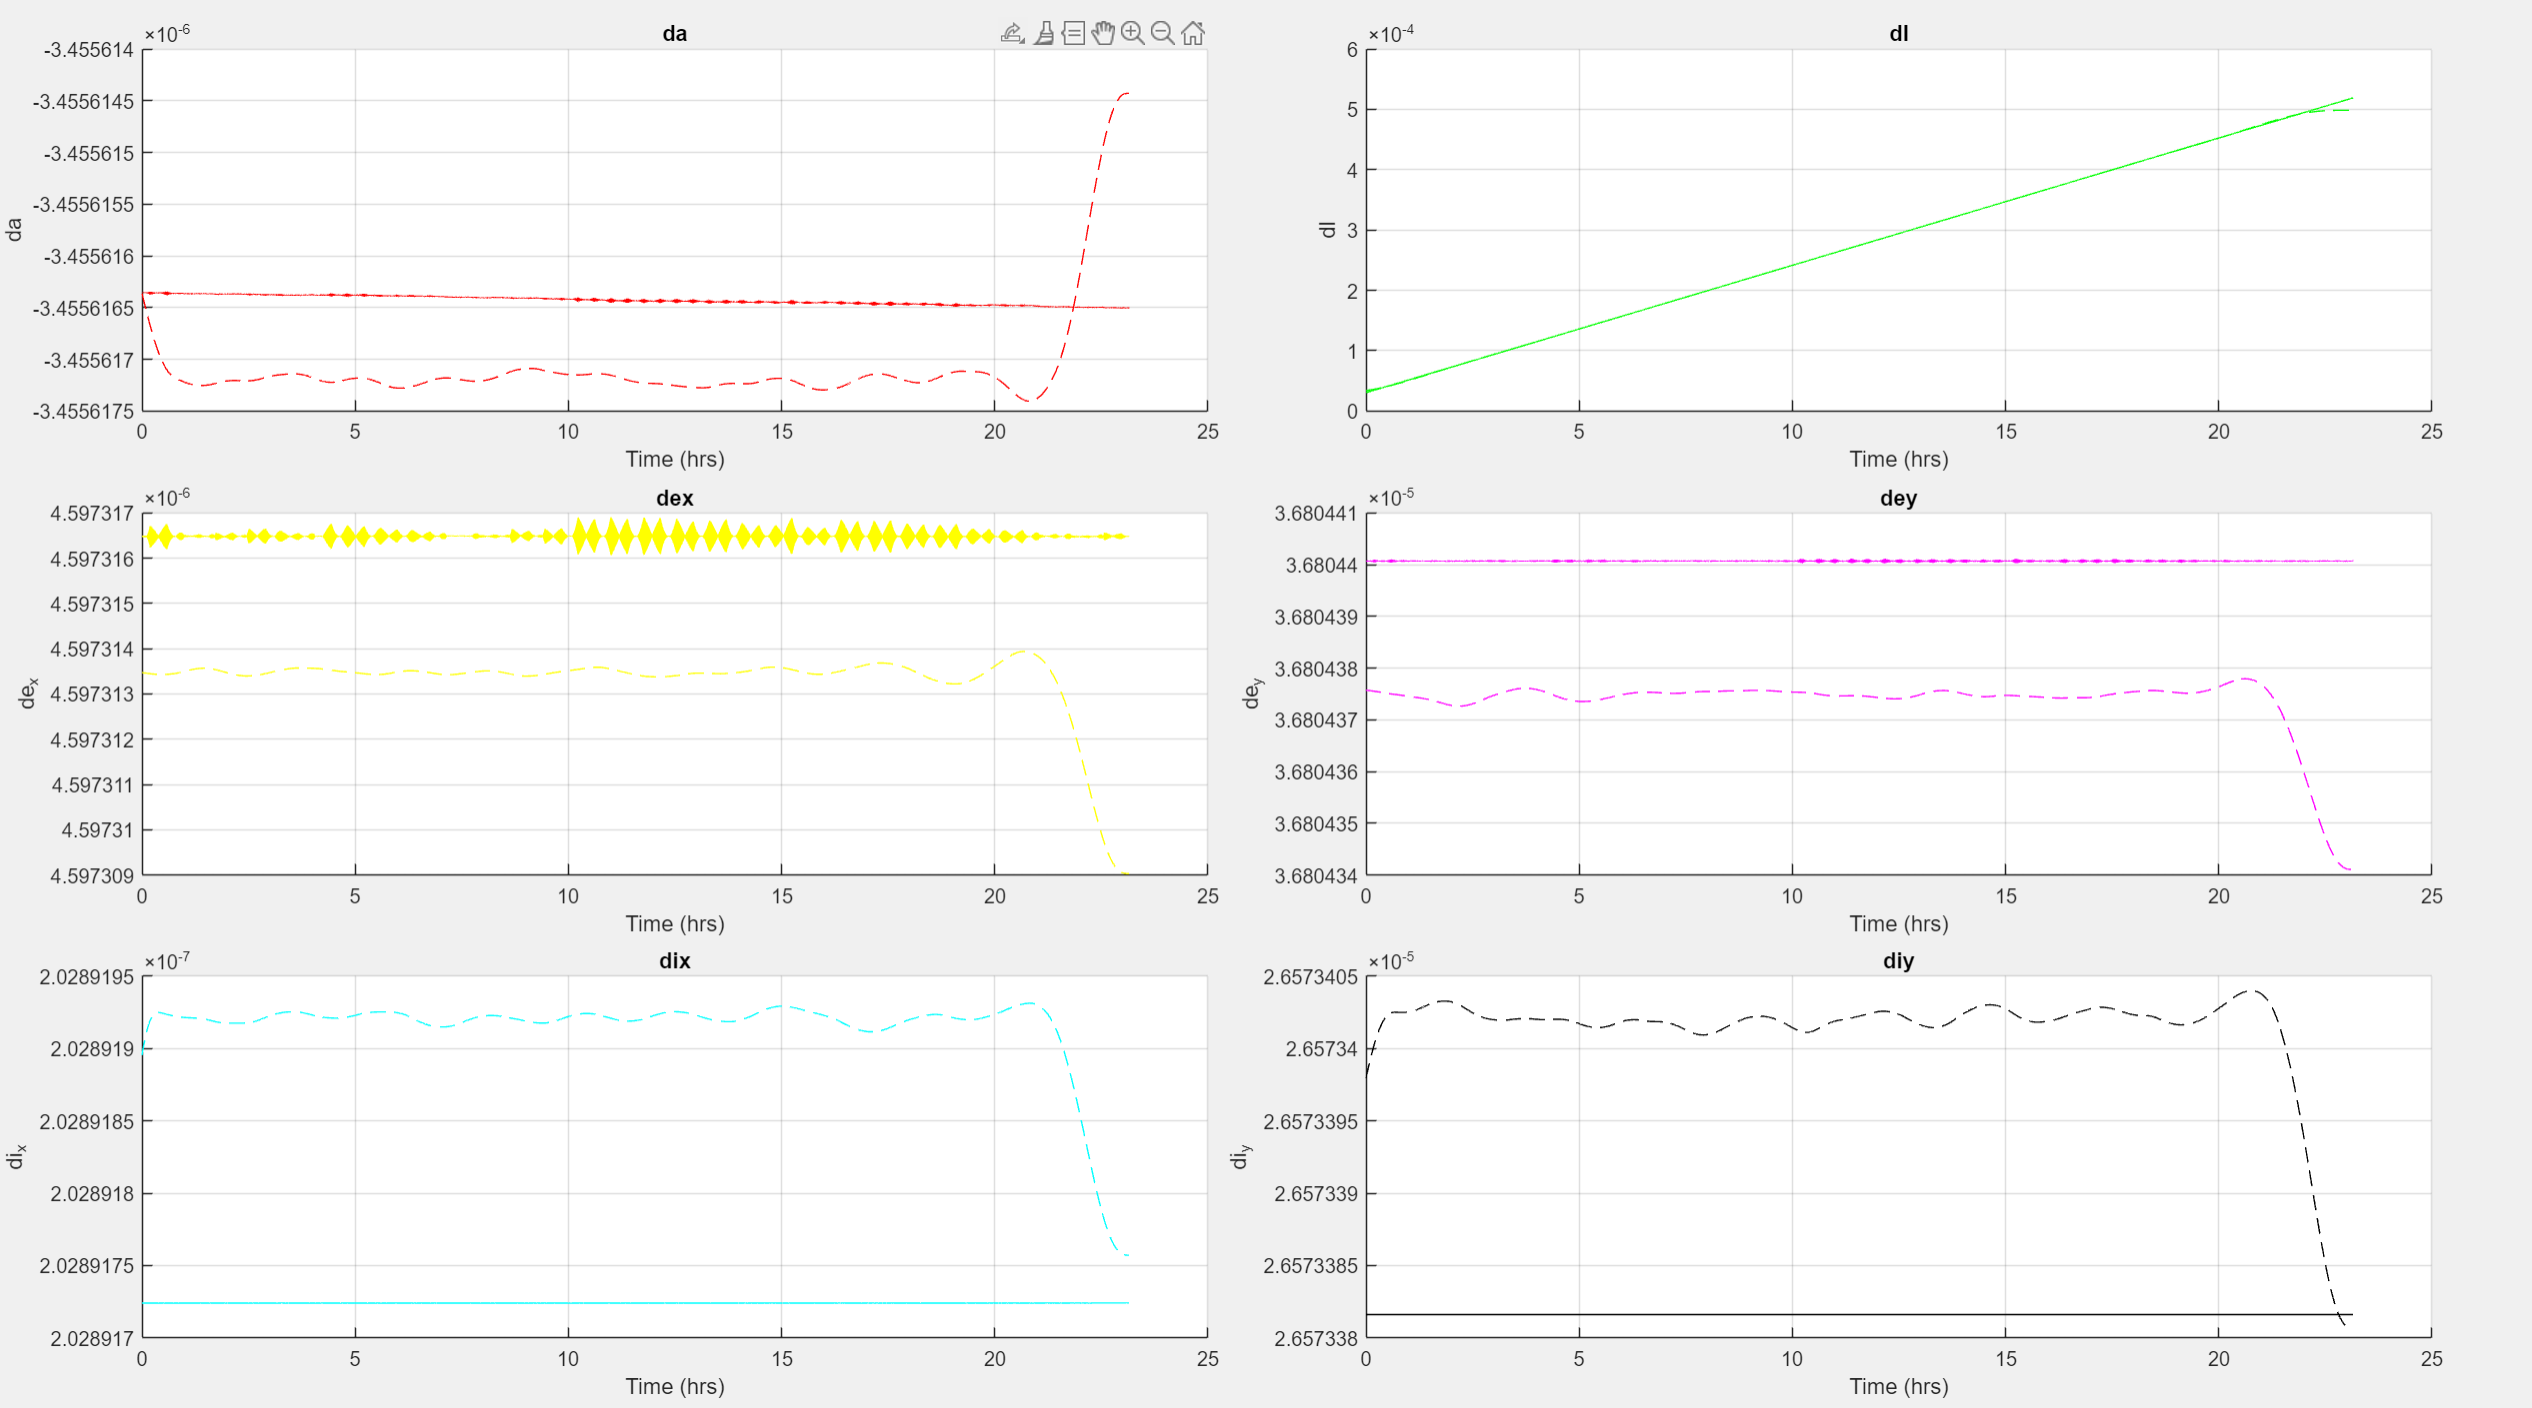
\includegraphics[width=0.7\textwidth]{PS4/Figures/case1_noJ2_2.png}
    \caption{Initial Conditions 1, Without J2, Quasi Nonsingular Relative Orbital Elements}
    \label{fig:hcw_velocity}
\end{figure}

First part, with J2:
\begin{figure}[H]
    \centering
    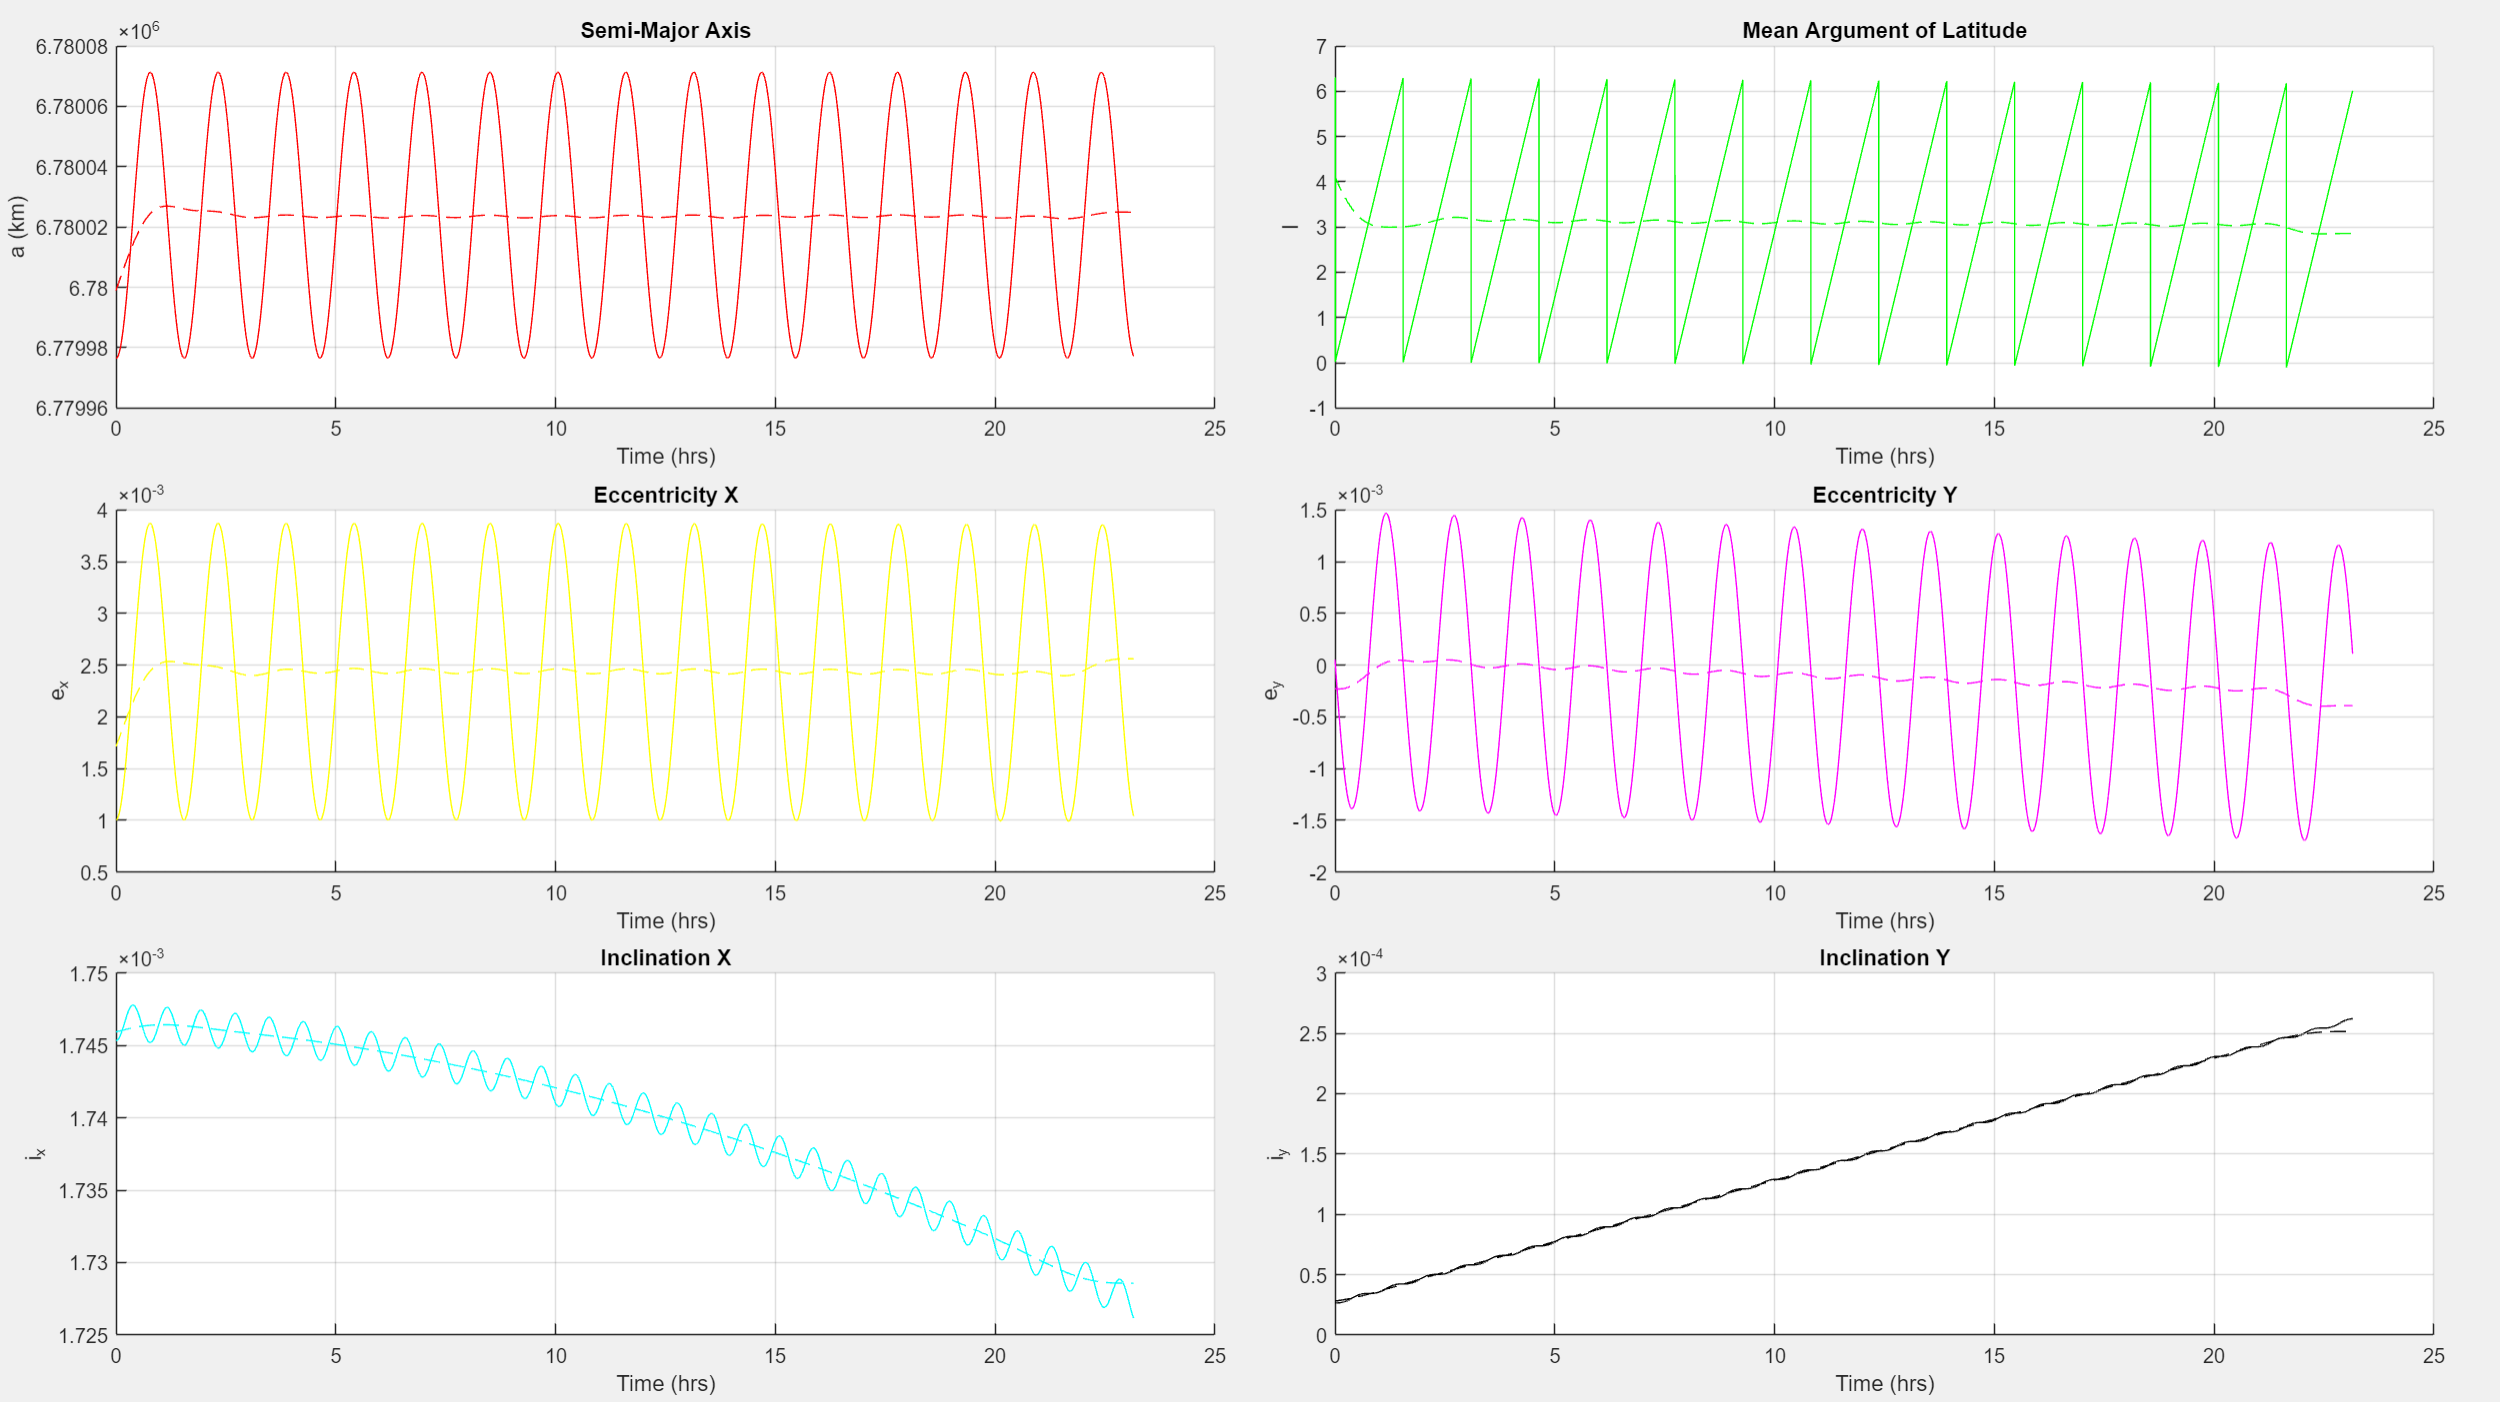
\includegraphics[width=0.7\textwidth]{PS4/Figures/case1_J2.png}
    \caption{Initial Conditions 1, With J2, Quasi Nonsingular Orbital Elements}
    \label{fig:hcw_velocity}
\end{figure}
\begin{figure}[H]
    \centering
    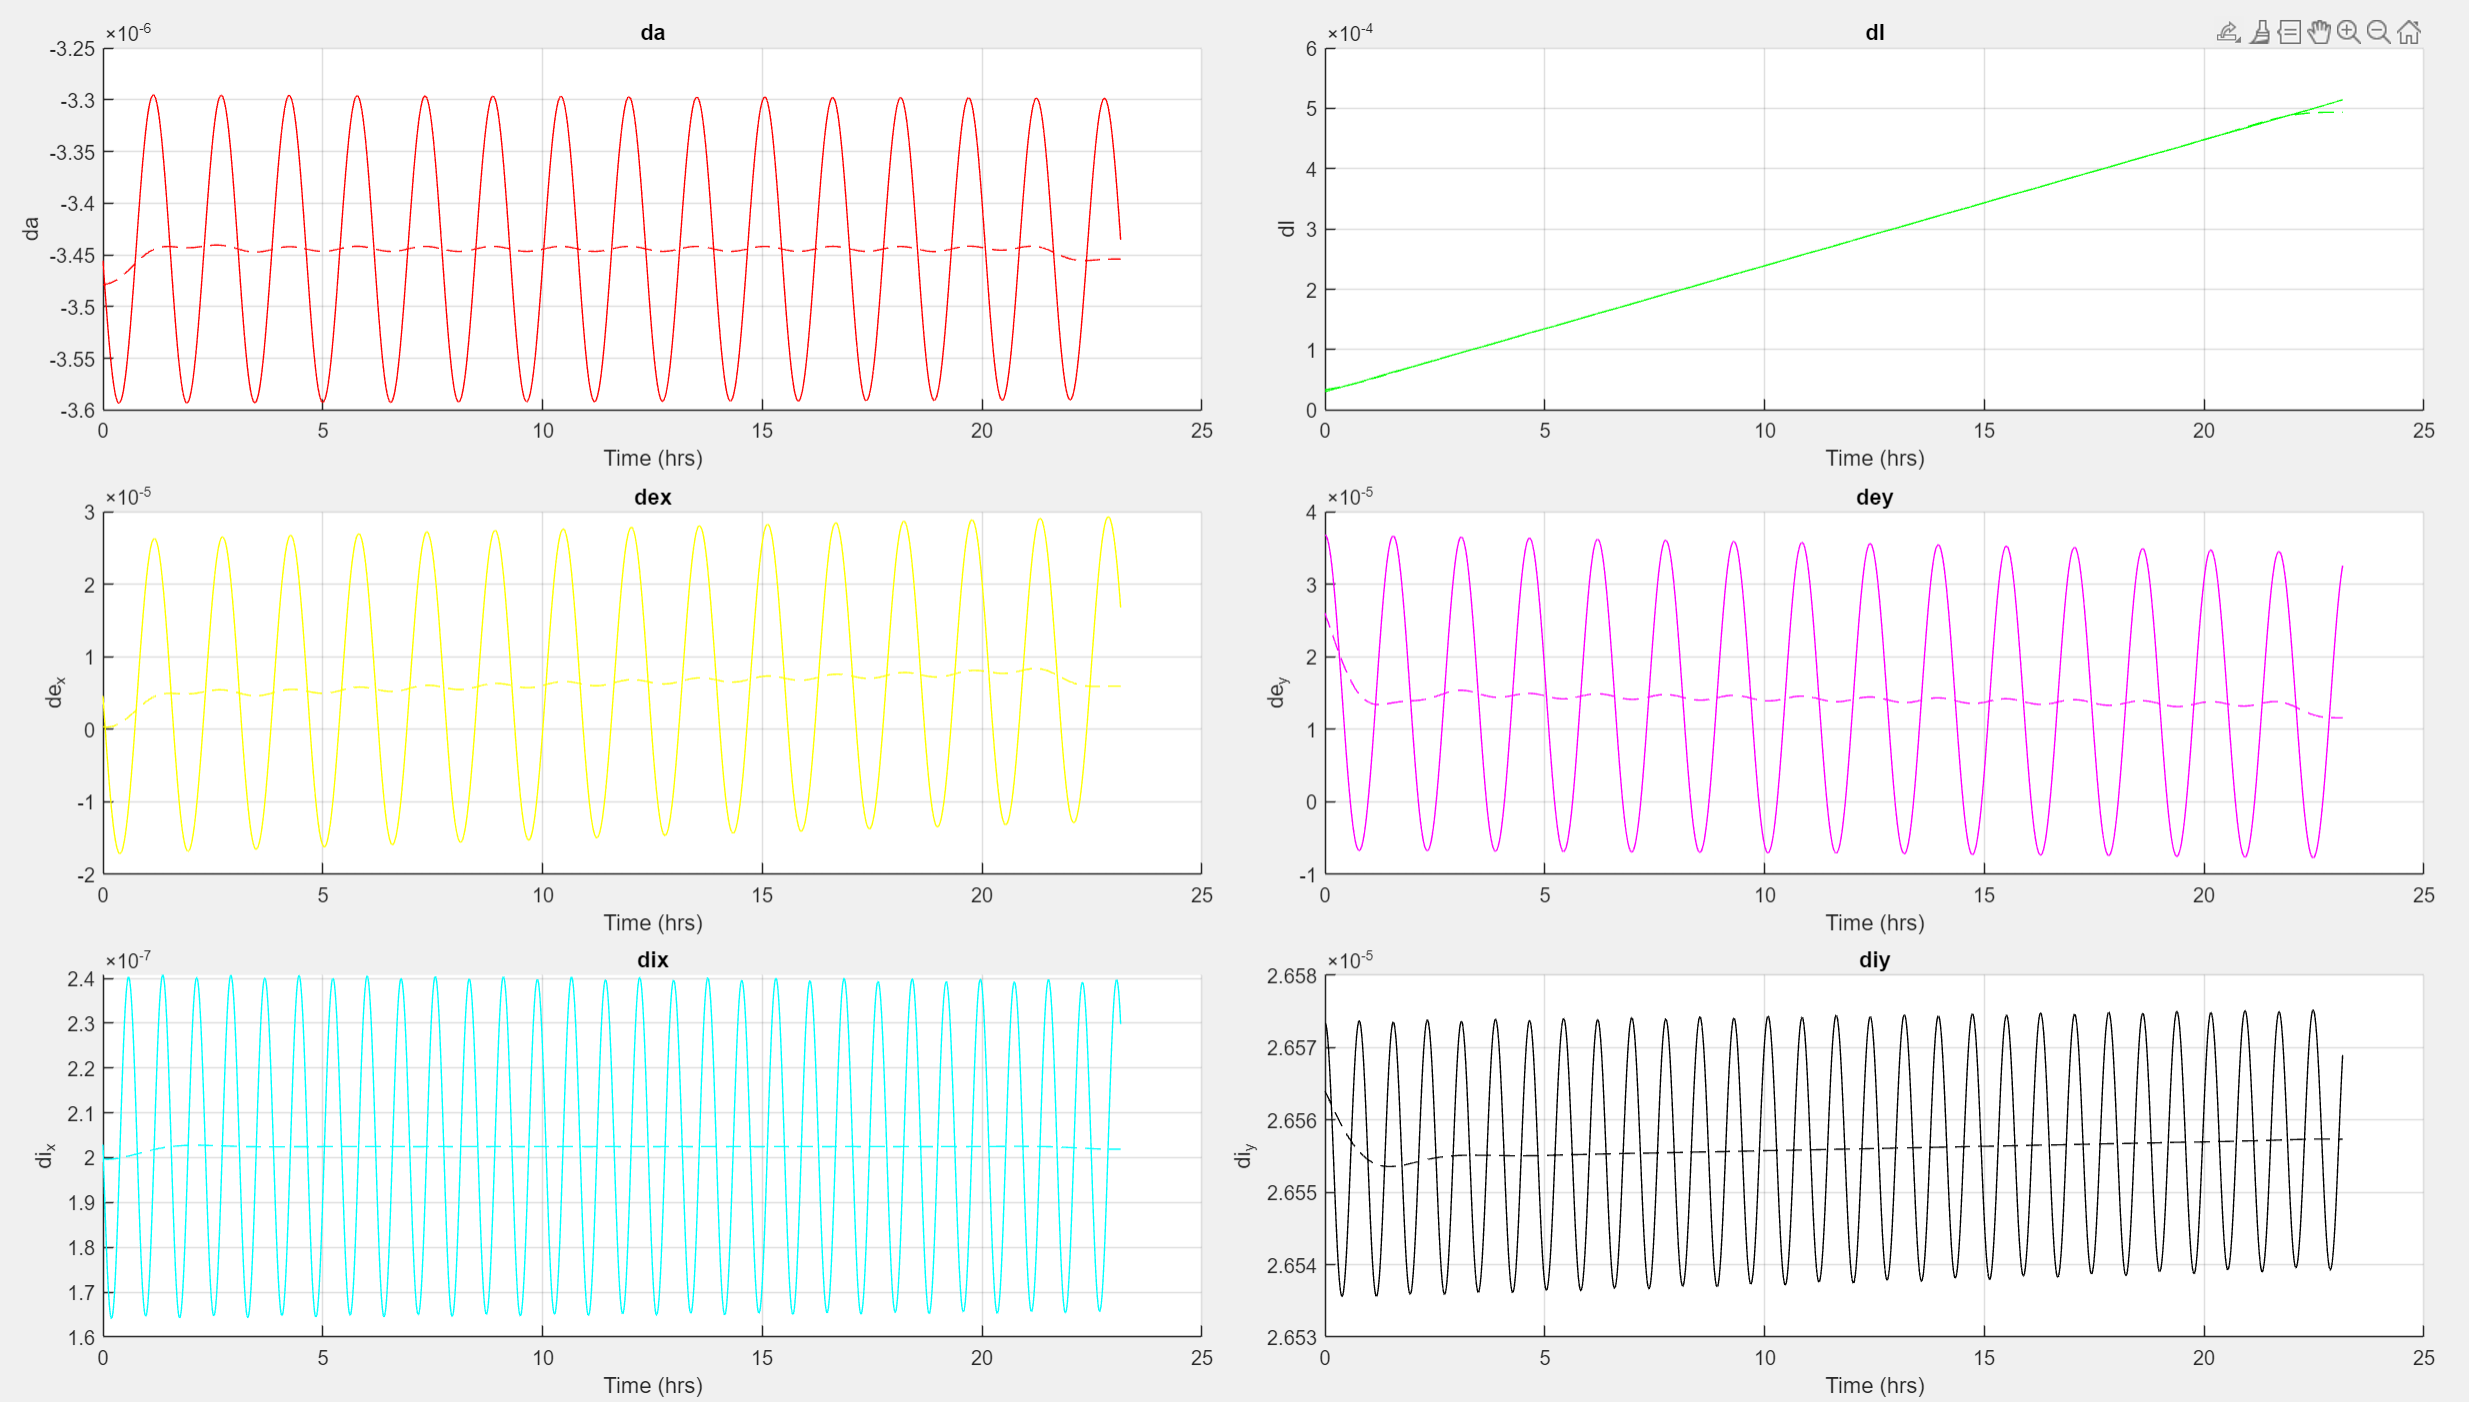
\includegraphics[width=0.7\textwidth]{PS4/Figures/case1_J2_2.png}
    \caption{Initial Conditions 1, With J2, Quasi Nonsingular Relative Orbital Elements}
    \label{fig:hcw_velocity}
\end{figure}
Second part, without J2:
\begin{figure}[H]
    \centering
    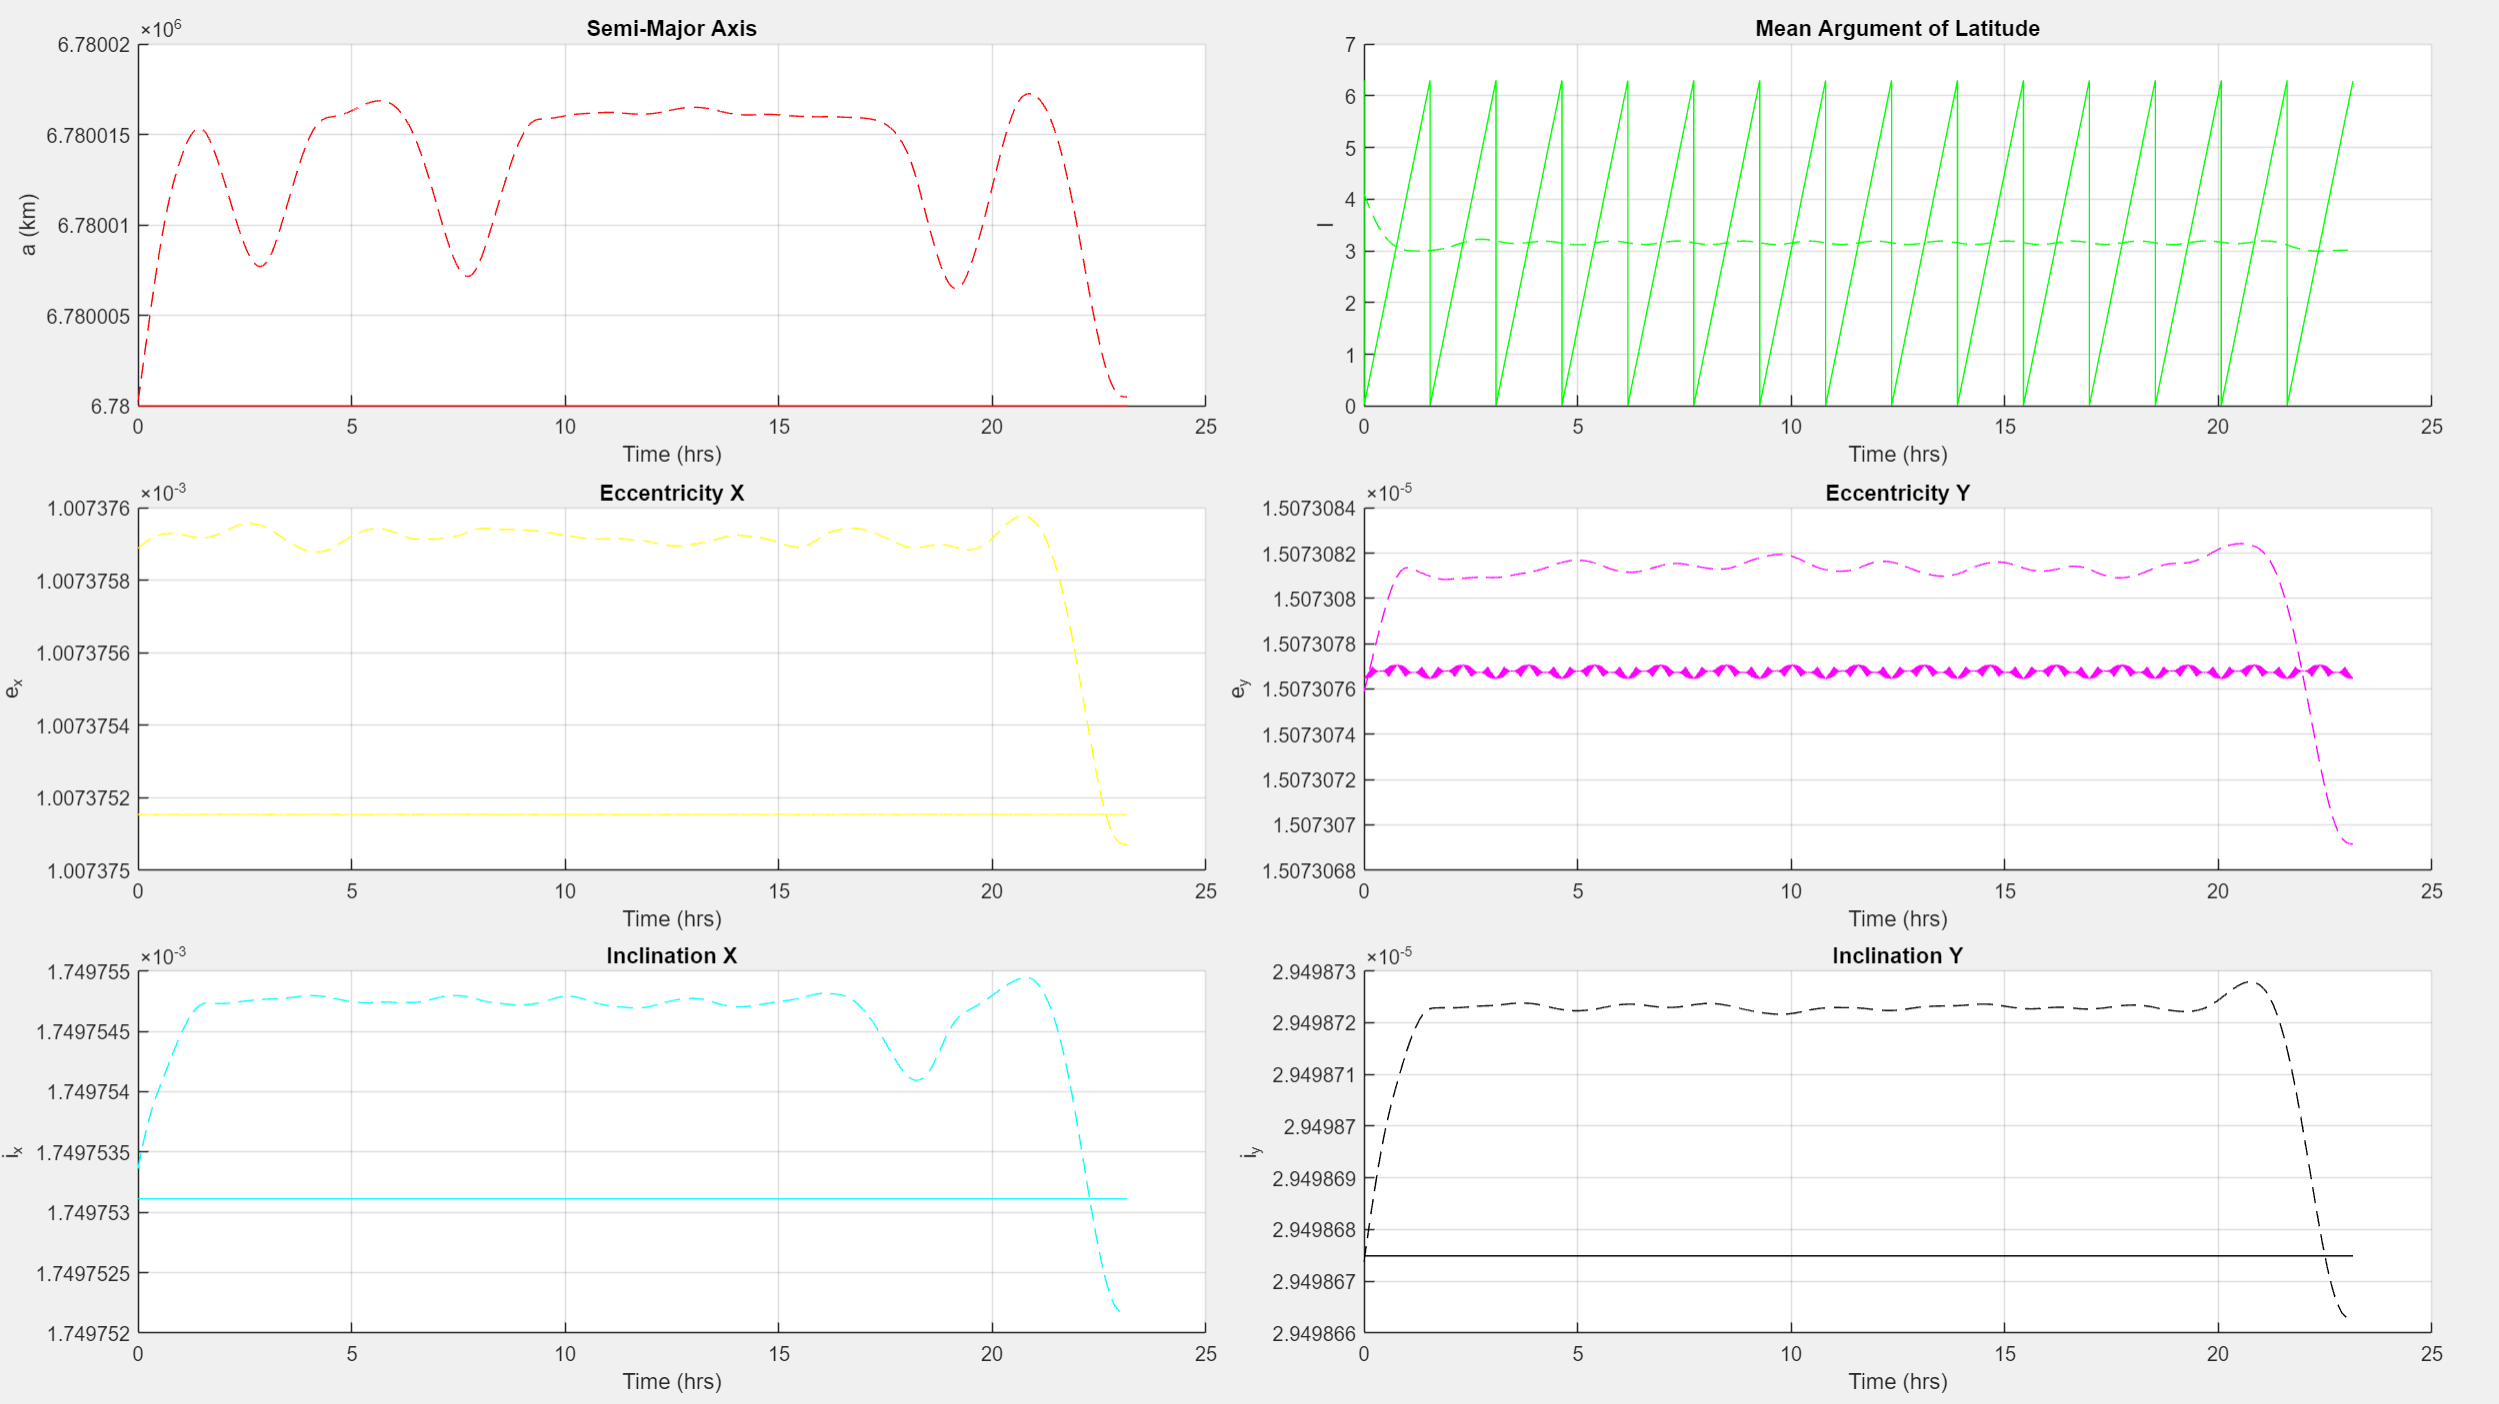
\includegraphics[width=0.7\textwidth]{PS4/Figures/case2_noJ2.png}
    \caption{Initial Conditions 2, Without J2, Quasi Nonsingular Orbital Elements}
    \label{fig:hcw_velocity}
\end{figure}
\begin{figure}[H]
    \centering
    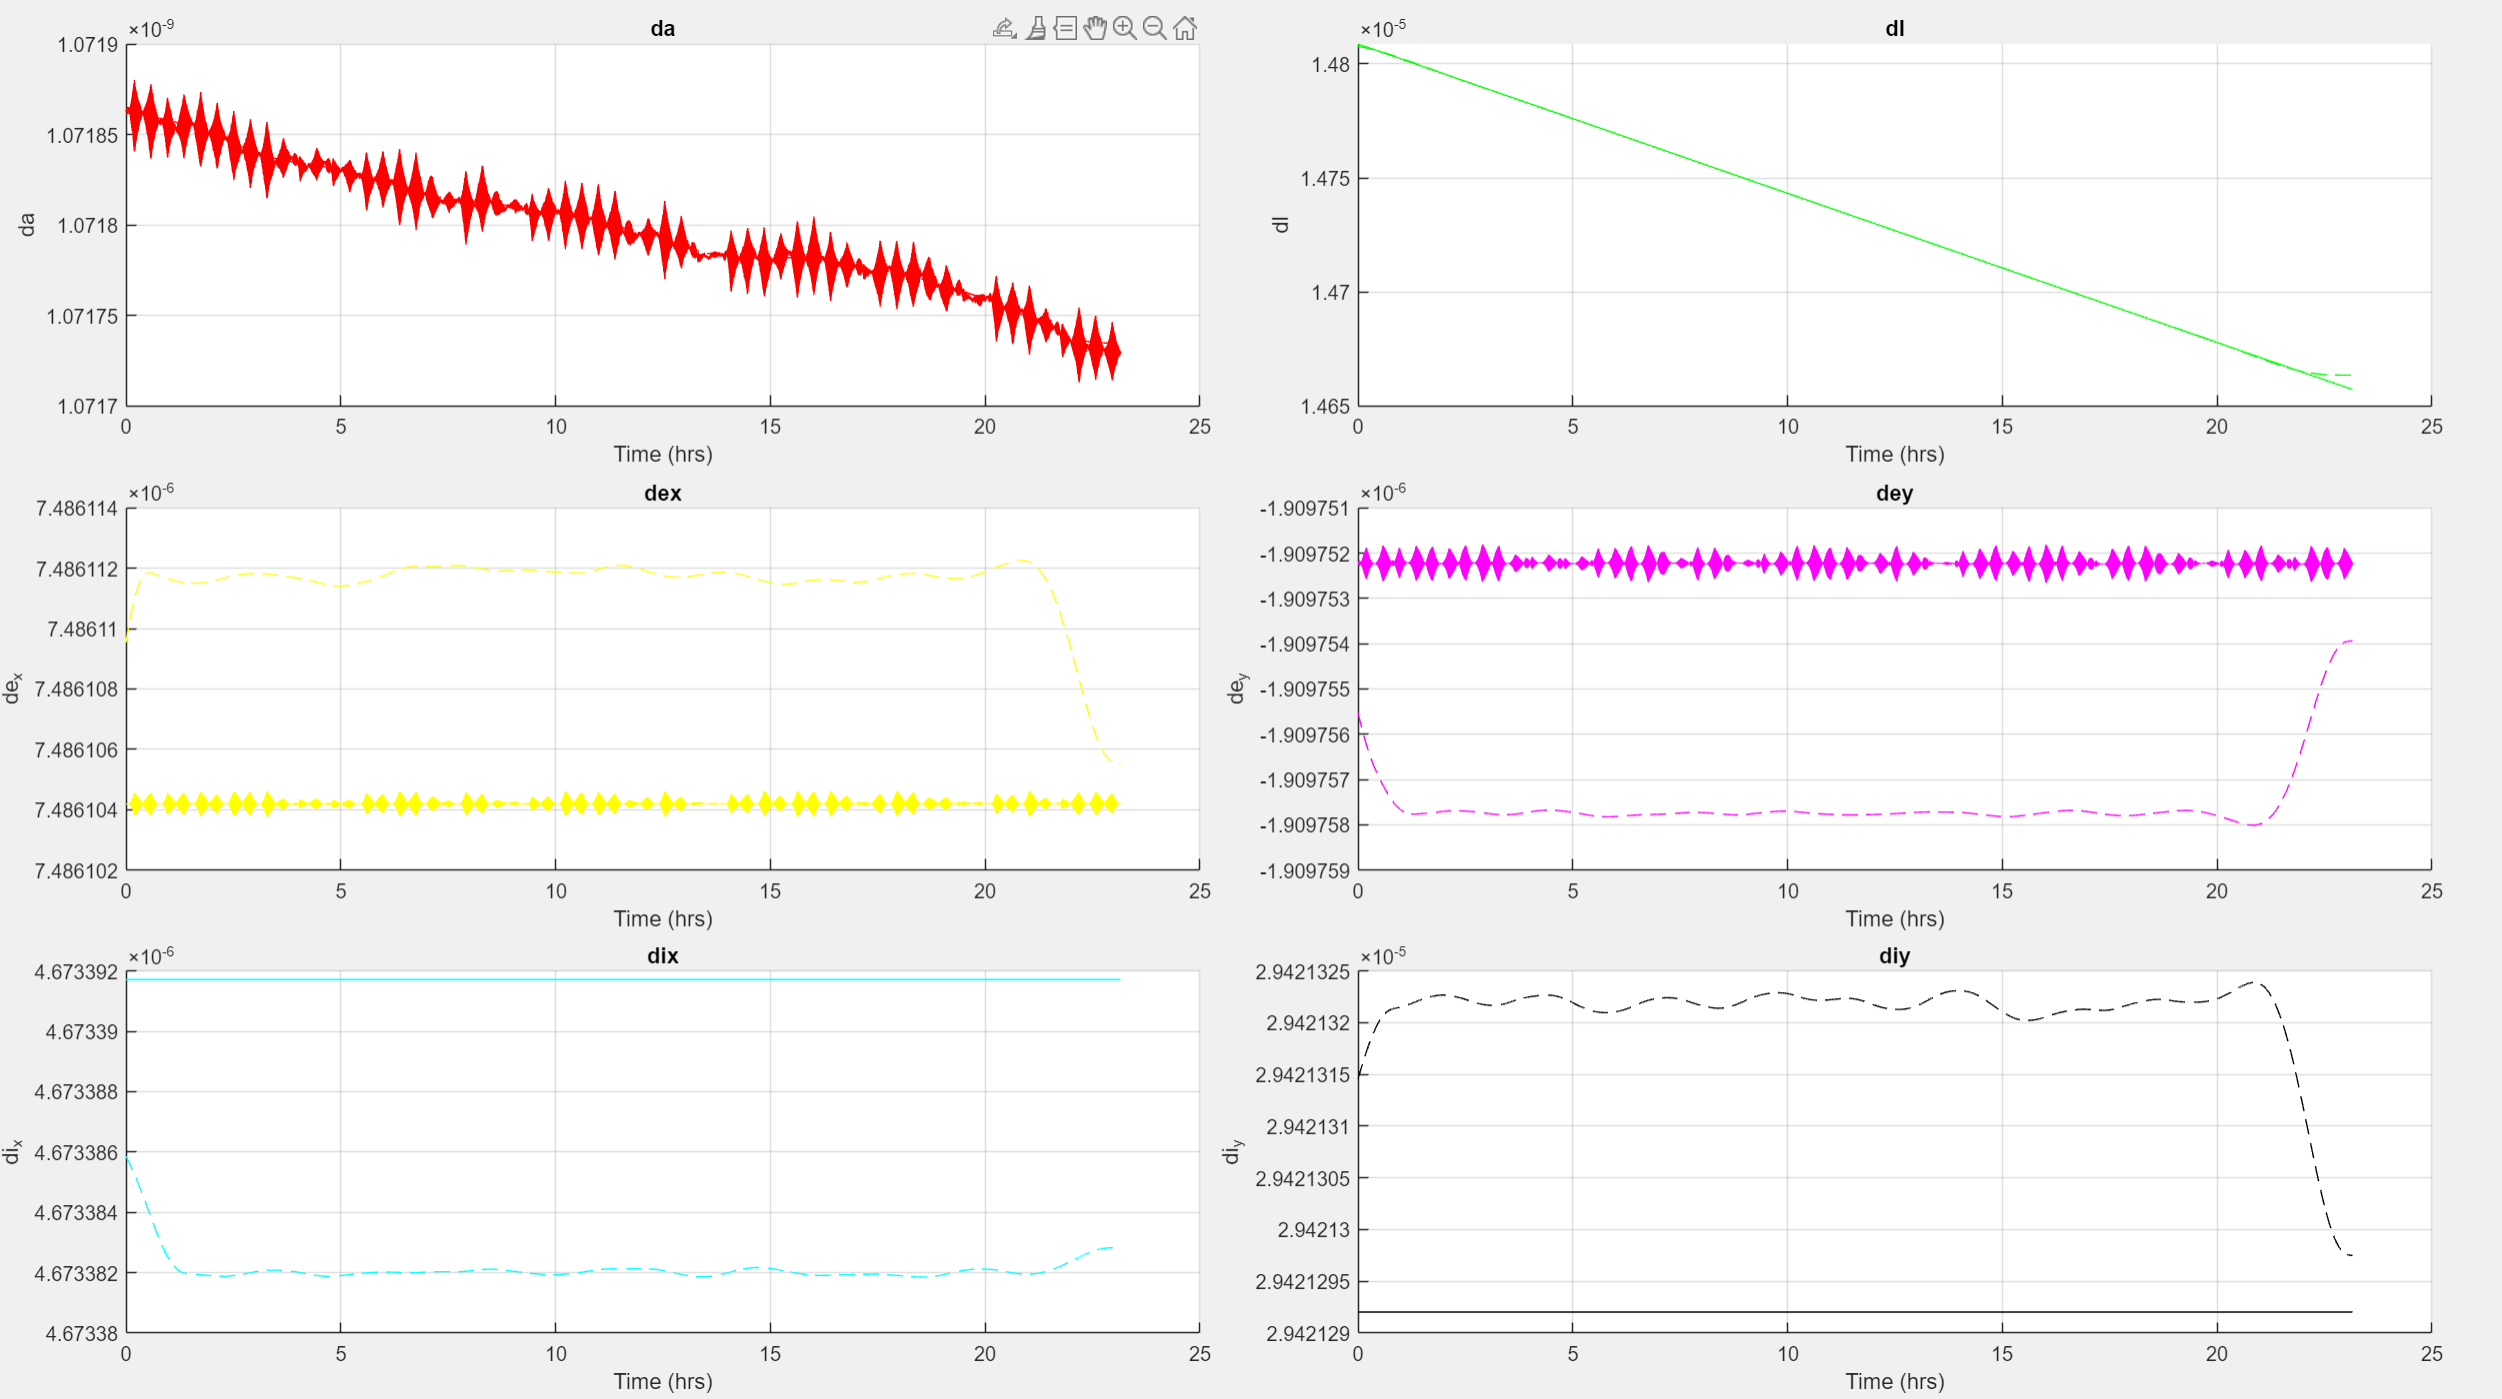
\includegraphics[width=0.7\textwidth]{PS4/Figures/case2_noJ2_2.png}
    \caption{Initial Conditions 2, Without J2, Quasi Nonsingular Relative Orbital Elements}
    \label{fig:hcw_velocity}
\end{figure}
Second part, with J2:
\begin{figure}[H]
    \centering
    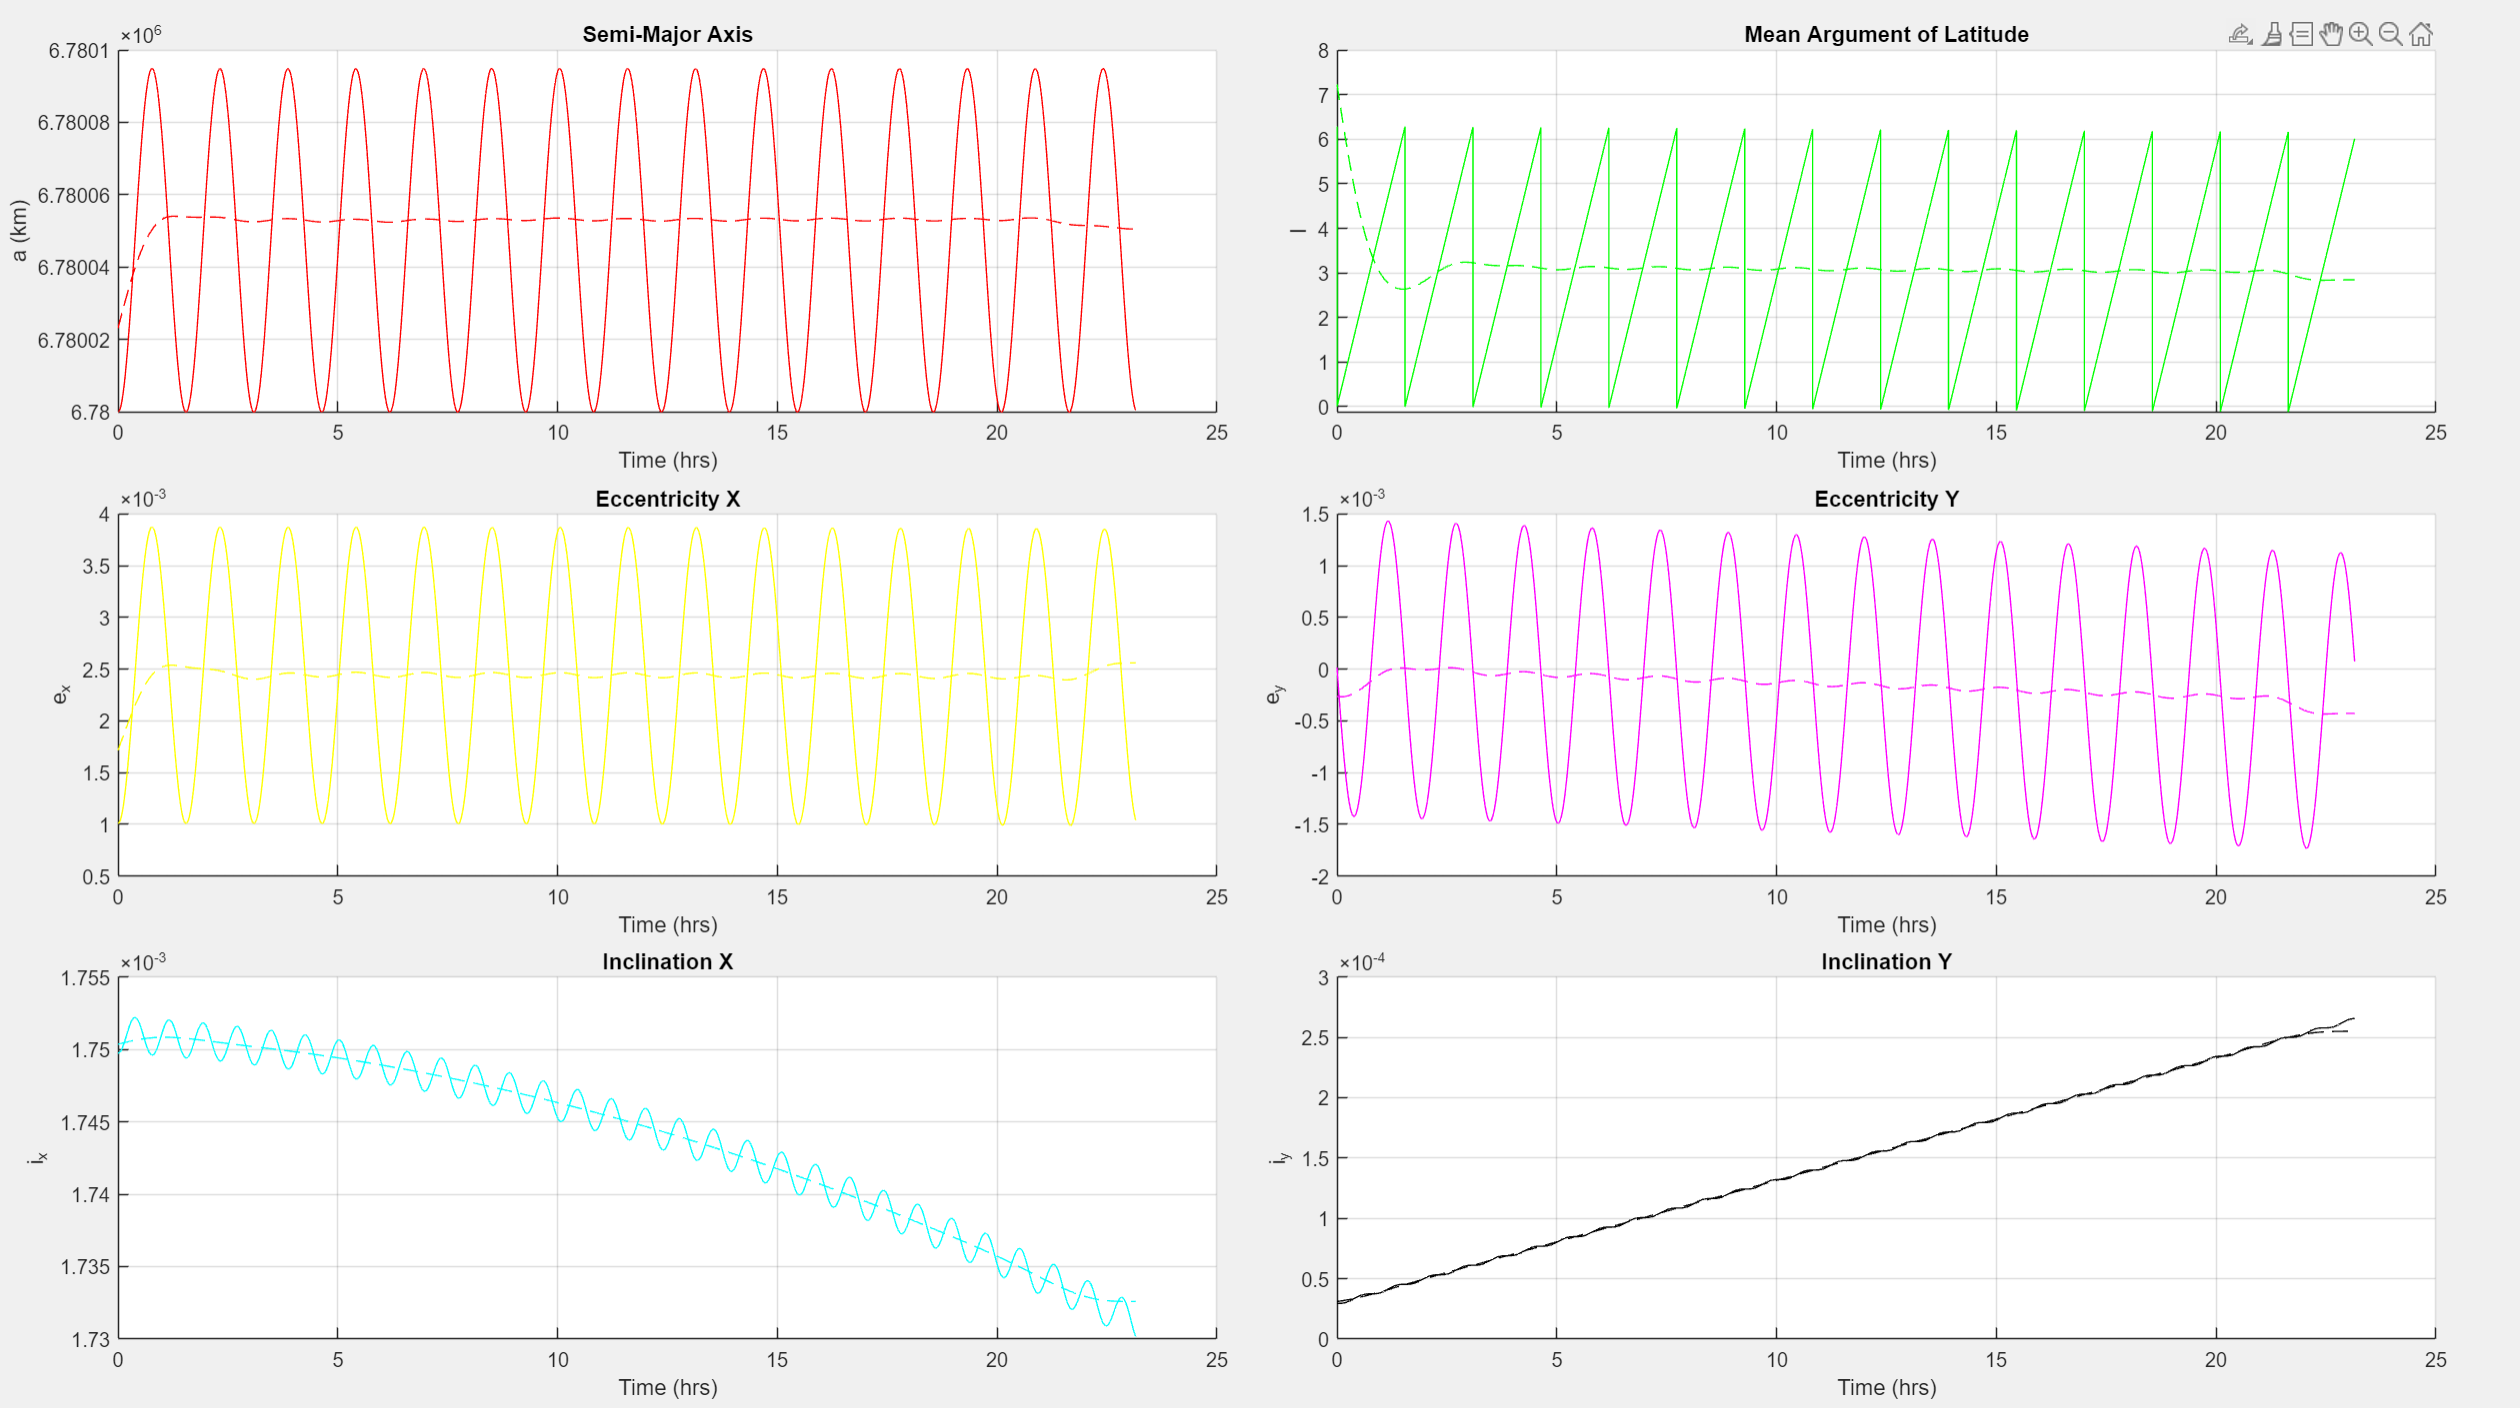
\includegraphics[width=0.7\textwidth]{PS4/Figures/case2_J2.png}
    \caption{Initial Conditions 2, with J2, Quasi Nonsingular Orbital Elements}
    \label{fig:hcw_velocity}
\end{figure}
\begin{figure}[H]
    \centering
    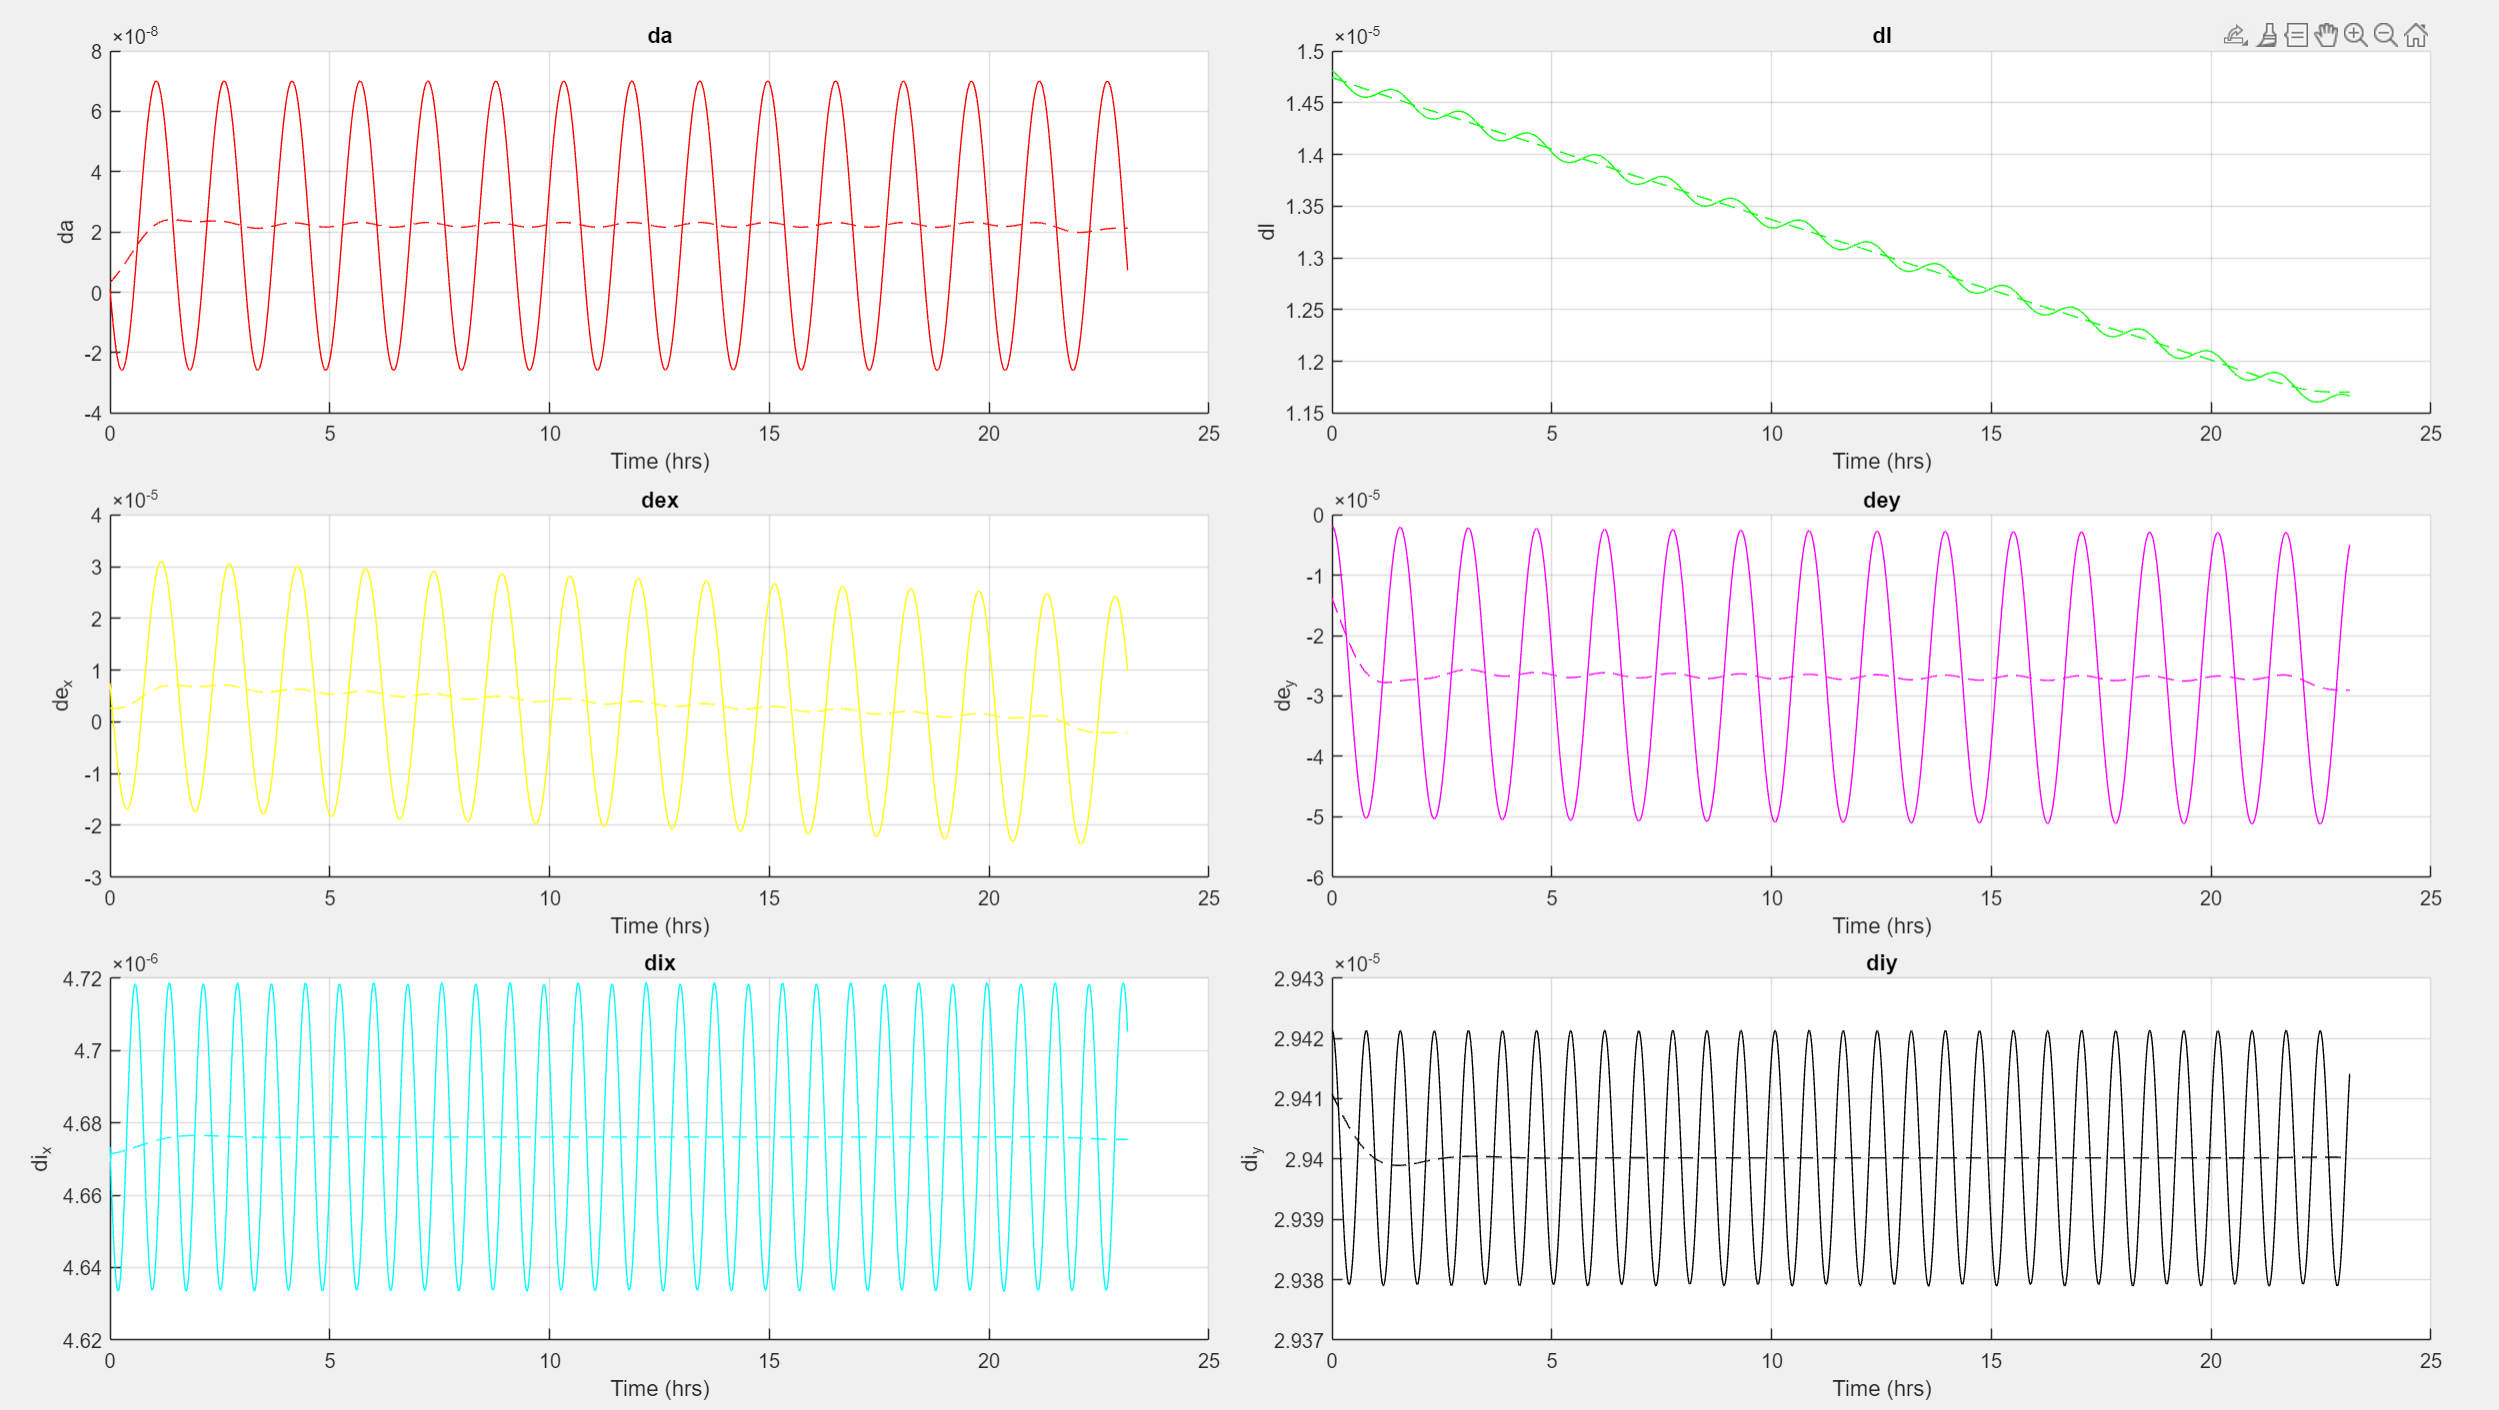
\includegraphics[width=0.7\textwidth]{PS4/Figures/case2_J2_2.png}
    \caption{Initial Conditions 2, with J2, Quasi Nonsingular Relative Orbital Elements}
    \label{fig:hcw_velocity}
\end{figure}

\subsubsection{Simulation with and without J2}
\begin{figure}[H]
    \centering
    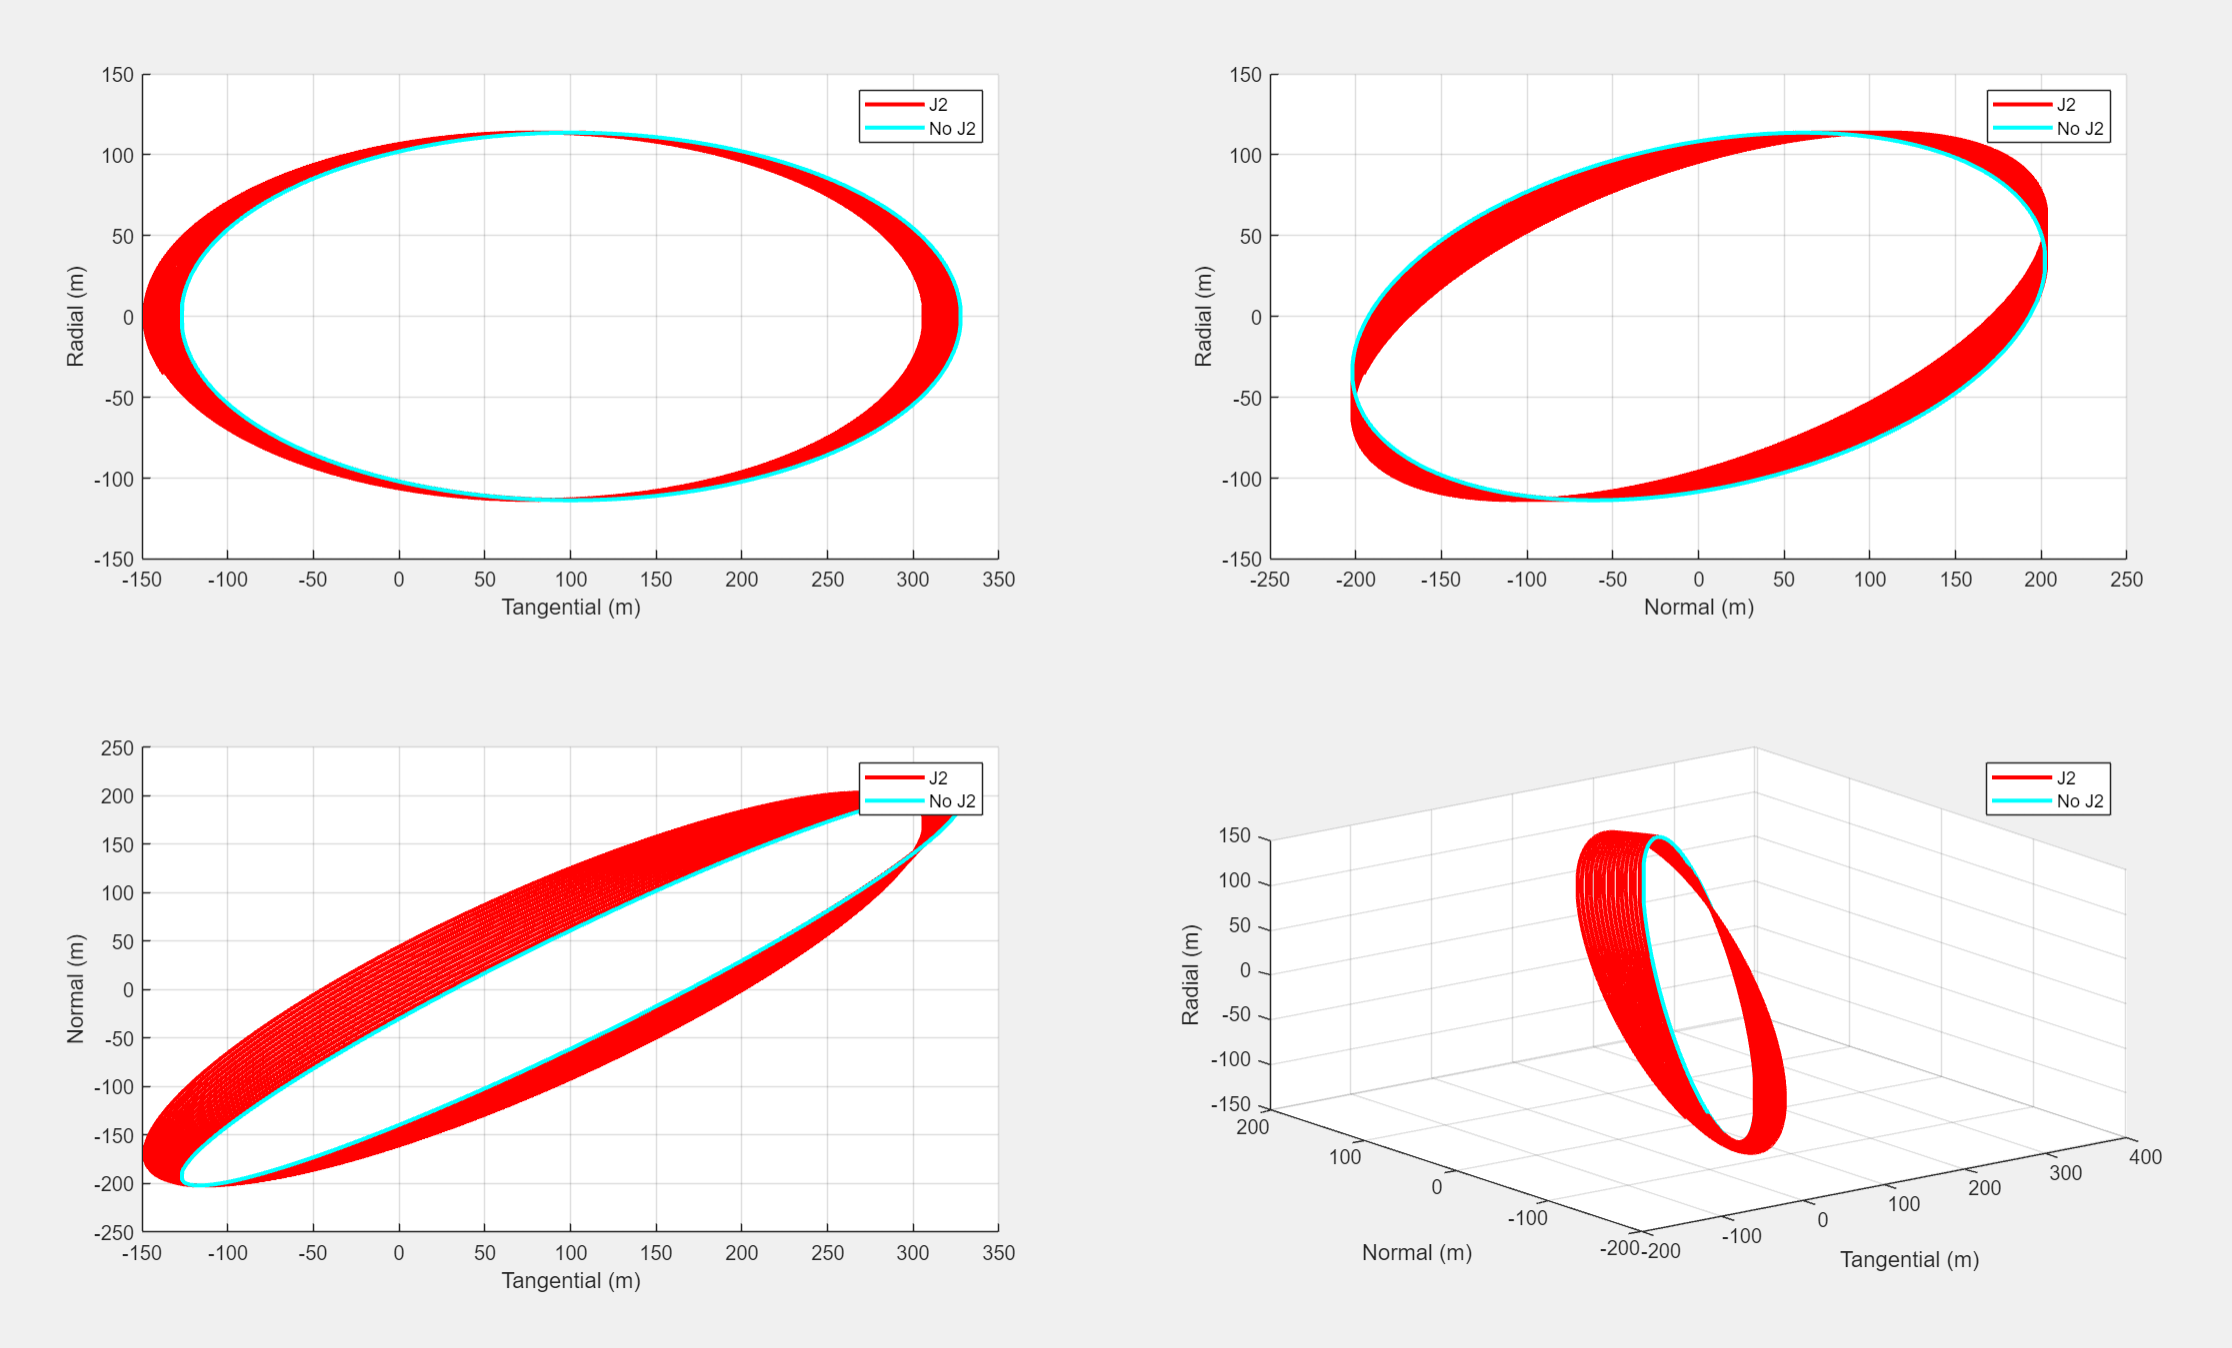
\includegraphics[width=0.7\textwidth]{PS4/Figures/rtn_position.png}
    \caption{RTN Position}
    \label{fig:hcw_velocity}
\end{figure}
\begin{figure}[H]
    \centering
    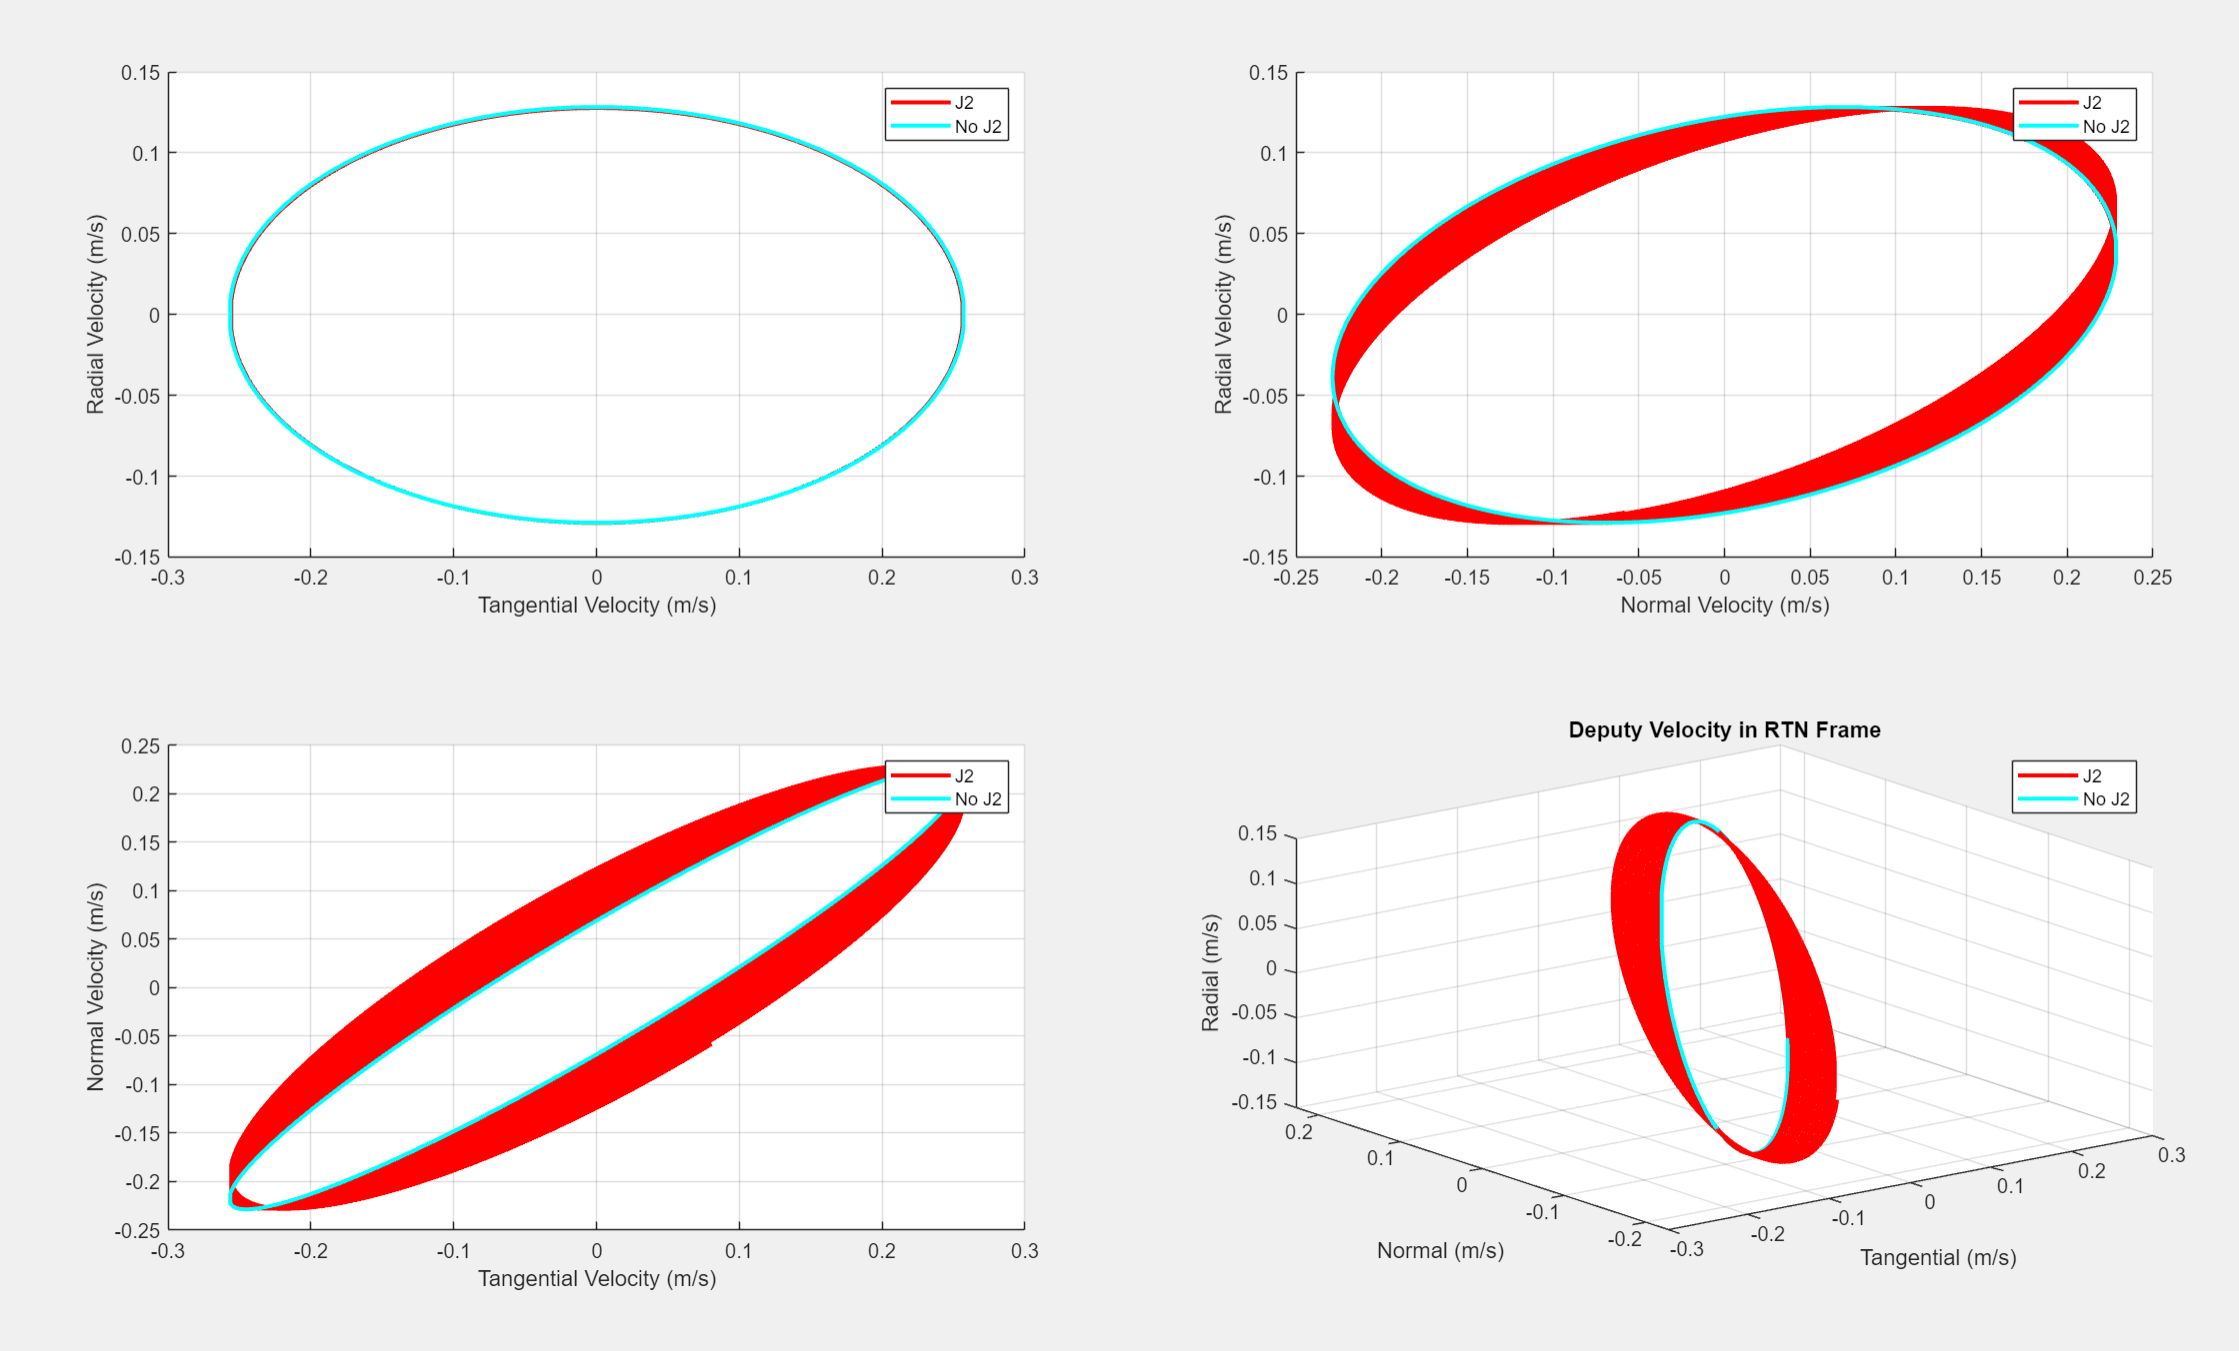
\includegraphics[width=0.7\textwidth]{PS4/Figures/rtn_velocity.png}
    \caption{RTN Velocity}
    \label{fig:hcw_velocity}
\end{figure}

\subsubsection{Planar Plots with J2 Effects}
In the following plots, the solid lines are the osculating and the dotted lines are the means.
\begin{figure}[H]
    \centering
    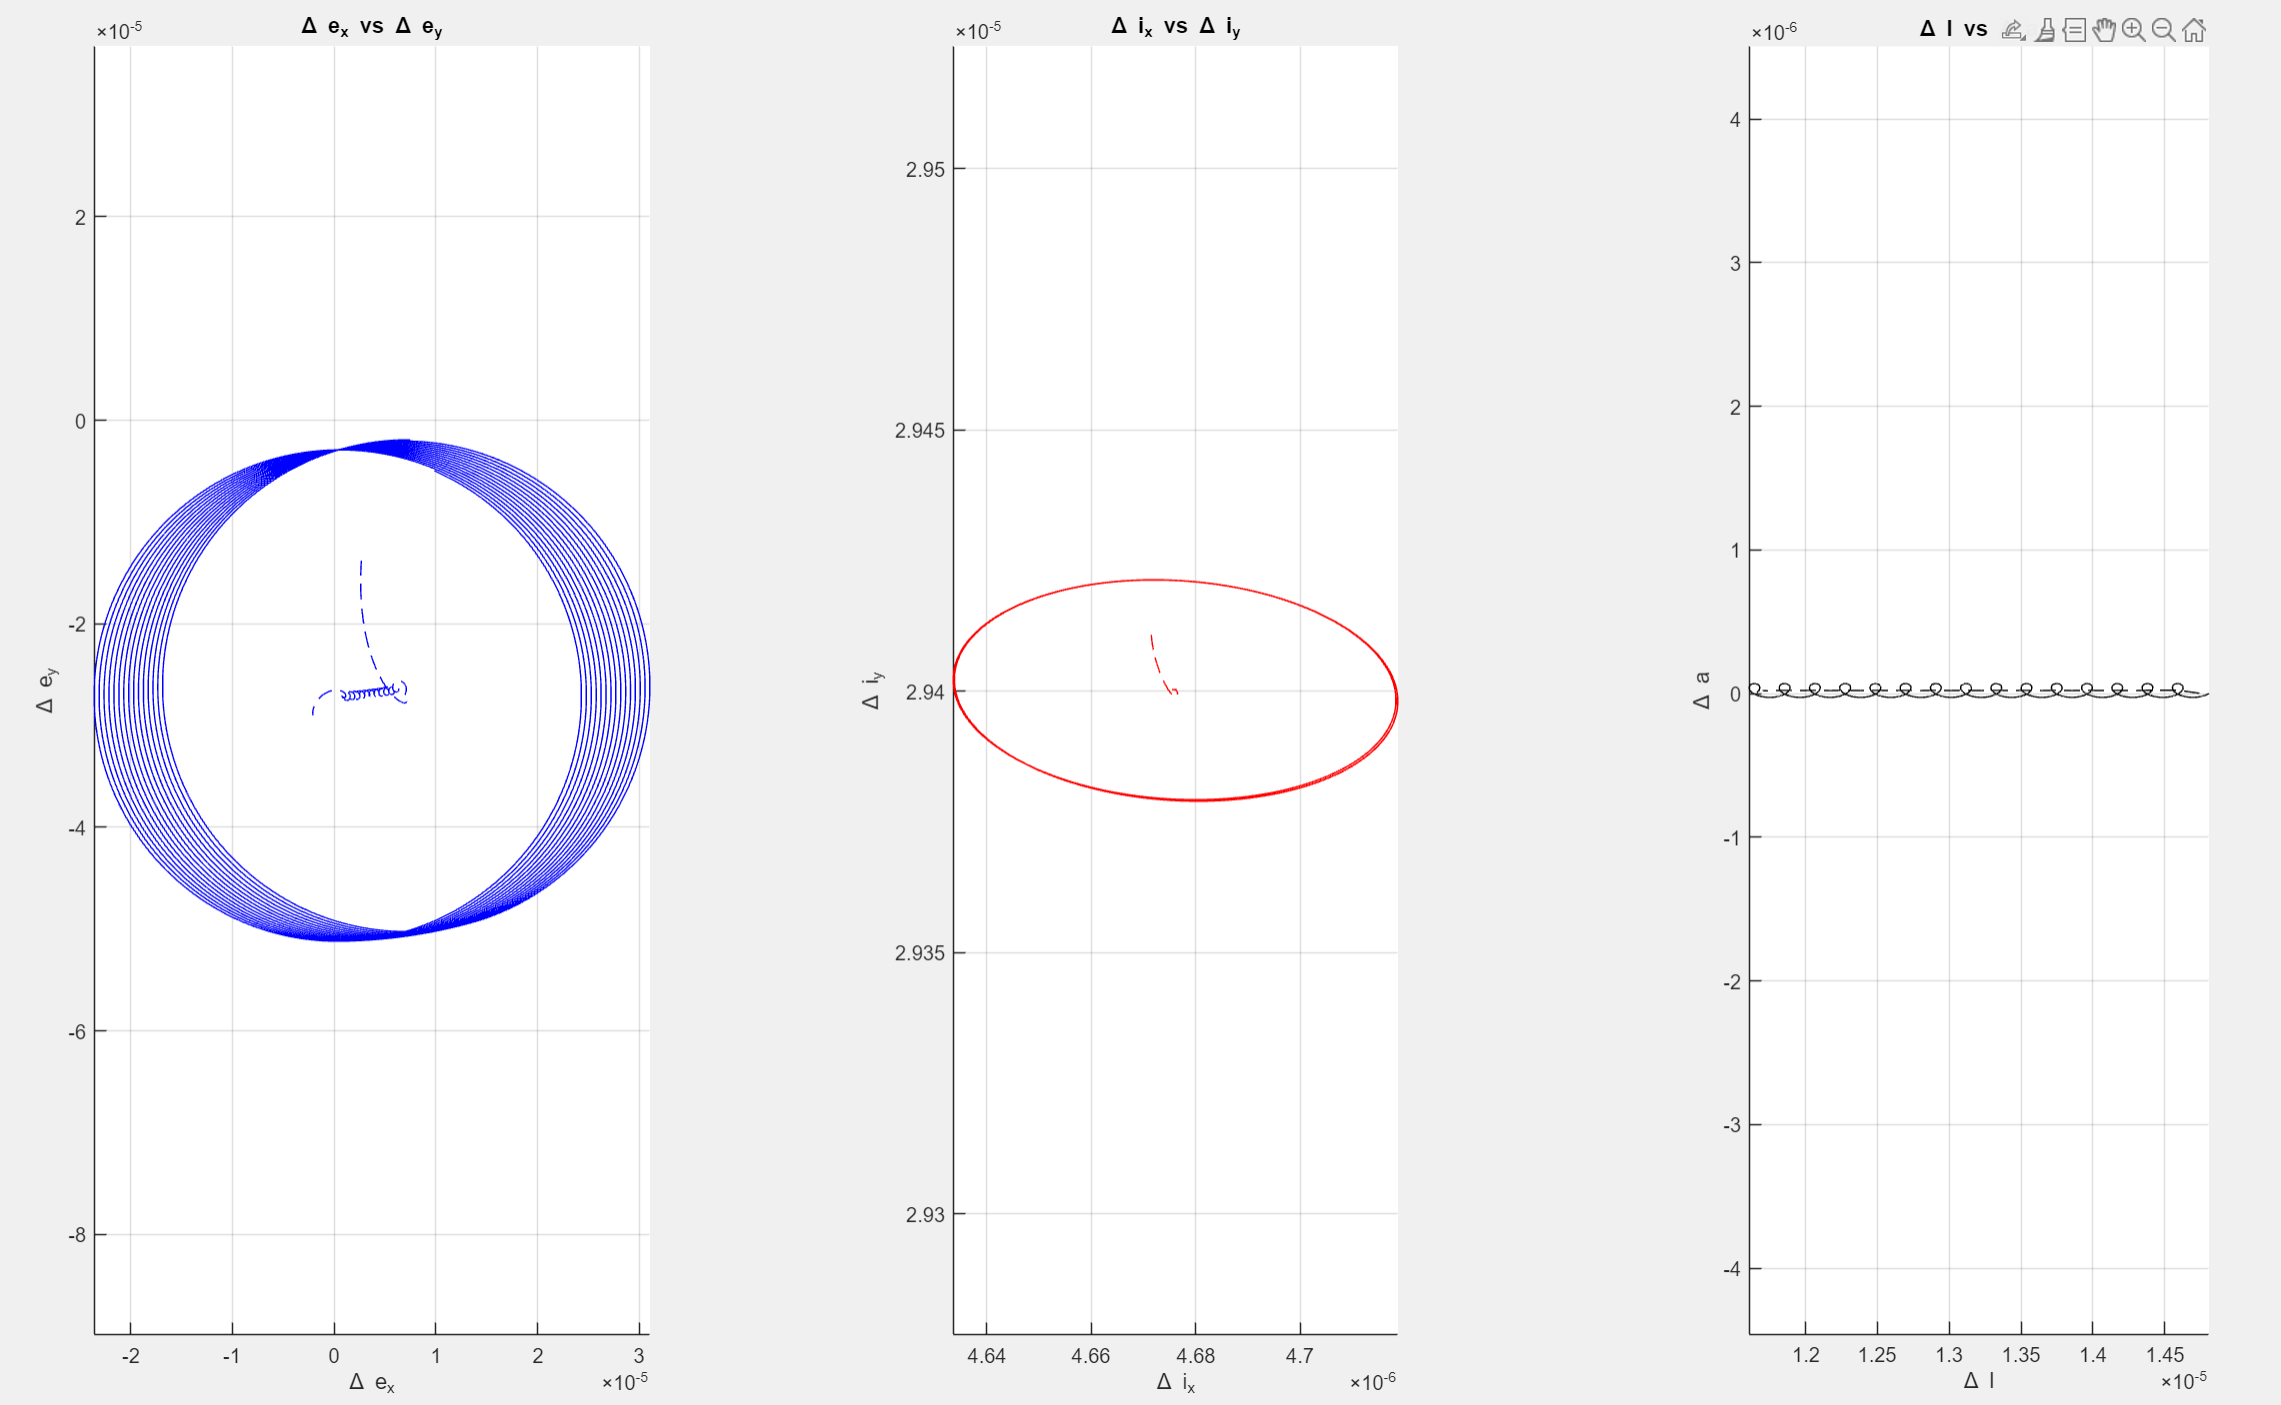
\includegraphics[width=0.7\textwidth]{PS4/Figures/problem5.png}
    \caption{Planar Plots of Roes over Time with J2 effects}
    \label{fig:hcw_velocity}
\end{figure}

\subsubsection{Drift Due to J2}
As Professor D'Amico discussed in class, one could leverage a difference in specific mechanical energy to cancel J2. If the da orbital element is approximately equal to 1000 times the differential inclination elements, the effect of J2 will negate the keplerian drift, thus rendering a stable situation. 

To do this with our initial conditions, we start with the equation $\delta \lambda' = -\frac{21}{2} \left( \gamma \sin(2i)\, \delta i_x + \frac{1}{7} \delta a \right)$. By substituting in our known inclination, a zero change rate of delta lambda, and our known inclination component in the x direction, we can obtain a delta a of 10.43m. Therefore, we must increase our semi major axis by 10.43m, which translates to a prograde burn with a delta v of 9.51 m/s. These calculations were done by using the necessary change in semi major axis and the vis a via equation. When we re-ran our simulation with these new initial conditions we saw that the secular effects were almost entirely removed.


\subsubsection{Adding STM J2 effects}

The plot below shows the comparison between numerical integration and analytical STM solution.

\begin{figure}[H]
    \centering
    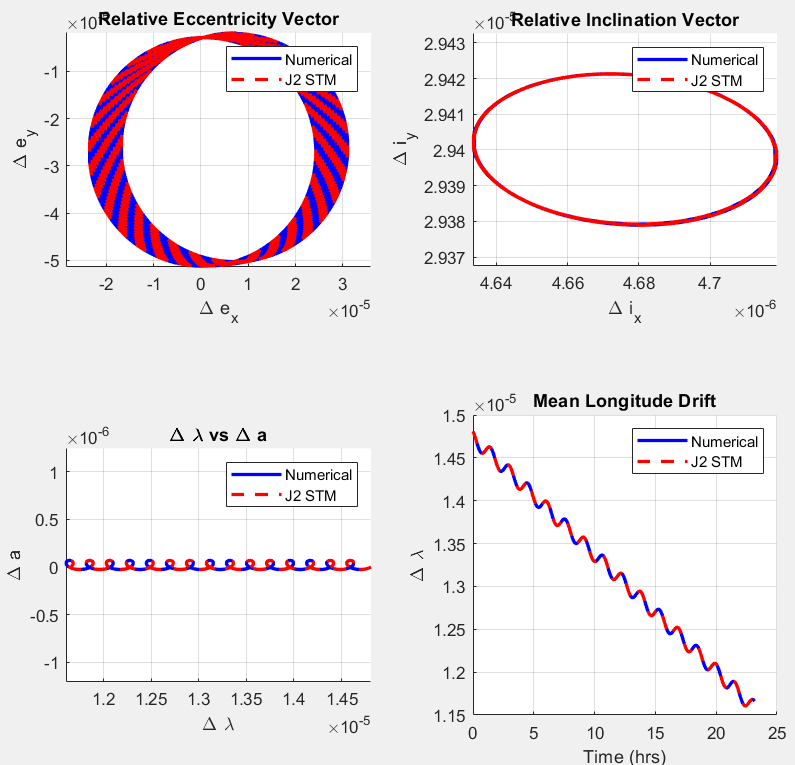
\includegraphics[width=0.7\textwidth]{PS4/Figures/ROE_STM_Comparison.png}
    \caption{STM J2 comparison.}
    \label{fig:stm_comparison}
\end{figure}{

\newpage
\section{Problem Set 5}

\subsection{What are the Control Objectives?}

\subsubsection{Significant Operational Modes}
The most significant operational modes of our mission will be station keeping, docking, and safety. As with all scientific missions, station keeping will occur when the spacecrafts are not required to do any observation or function, but rather hold position while other mission objectives are being accomplished, such as generating power or transmitting data. From a distributed space systems perspective, station keeping will require the spacecraft to maintain a stable configuration, sometimes in the vicinity of of the ISS. Therefore, it will be required to hold the same energy state and same semi major axis.

The next mode to consider is docking mode, where the dragon is moving itself closer to the ISS. This mode requires an inherent instability and difference in semi major axis, where an approach is being made purposefully.

Finally, the last mode is safety mode, which also includes a difference in semi major axis because the dragon should back away from the station in this scenario. It does not necessarily have to be fast, but rather, safety will come in the assured slow drift away.

\subsubsection{Specific Constraints on Operational Modes}
For station keeping, the most significant requirement is that the semi major axes must align to keep the energy state the same. Thus, the spacecraft will not have a meaningful drift away from each other if the orbits are mostly circular (which in this case they are). Given the space station's absolute orbital elements of [6780 km, 0.0006, 51.6 deg, 0 deg, 0 deg, 0 deg] the spacecraft dragon spacecraft may have a station keeping orbit of [6780 km, 0.0006, 51.6 deg, 0 deg, 0 deg, 1 deg]. It should be clarified that this is not the only station keeping orbit that would be allowed, since during the approach to the station there would be many different times and locations where station keeping may be desired, and many different ways to hold a stable configuration relative to the station. The most important factor is that the semi major axes are the same.

For docking, it is necessary to induce a drift toward the station. This can be done in a number of ways, but lets assume the dragon is lagging behind the station and is attempting to catch up. If the starting orbital elements of the deputy are as such: [6780 km, 0.0006, 51.6 deg, 0 deg, 0 deg, 1 deg] then a possible method of bringing them closer together would be to shrink the semi major axis of the deputy. For example, something like [6779 km, 0.0006, 51.6 deg, 0 deg, 0 deg, 1 deg] would move the spacecraft together.

The safety mode is the exact opposite, since we now want to drift the spacecraft apart. Given the same initial conditions, it would then be necessary to expand the semi major axis so that the deputy is slowly backing away.

\subsubsection{Operational Constraints}
A significant operational constraint this mission would have would be the limitations on fuel. Since Dragon would likely have a long mission with a crucial deorbit burn at the end, it is vital that unnecessary fuel is not wasted. Therefore, minimizing the number of burns would be crucial for mission success.

Another key operational constraint would be separation of Dragon and ISS. Given these are two crewed vehicles, maintaniing proper distance during the complex docking operation is crucial. Any control we induce must be totally fail safe - as in if the thruster sticks on, or doesn't turn off, there is never a risk of collision.

Finally, to that end, we must consider our relative dynamics carefully. For each phase of approach, it would be important to set clear bounds on relative distances and velocities, and to engage safe mode if those are violated. Naturally, given safe mode would require a burn, we must also consider the result of that burn shutting down early or late. The top priority in all of this is crew safety, and collision avoidance is one of the most crucial areas for that.

\subsubsection{Operational Constraints while Switching Modes}
As discussed above, there are additional concerns when switching modes. When moving out of each mode, a burn is required. Thus, it is safest to be moving out of station keeping mode since the situation is stable, and any delays or issues do not impact safety. The riskiest mode to move out of is approach mode, since any delay or thruster issue will have significant implications for collision avoidance. It's crucial that when switching out of approach mode, the burns are accomplished seamlessly.

\subsubsection{Actuators}
Given the nature of our mission, high thrust and short burn thrusters would be the most useful. This is for several reasons. First of all, given the human safety nature of this mission, the ability to quickly maneuver out of dangerous situations is crucial. Using weak but efficient thrusters would have difficulty accomplishing this. Additionally, docking itself requires precise quick movements to accomplish, so enough thrust to move around with agility is important.

\subsubsection{Sim setup}
The simulator that has been developed thus far should function well for this problem, since we can see both the absolute and relative orbital elements, as well as choose our propagation method. Since the eccentricity is small, HCW may be a sufficent method, but we will test and compare to see if there are significant differences between methods. We likely do not need to consider third body effects since we are in LEO, but J2 should be considered. Per usual, the pros of using simpler methods and disregarding perturbations are found in simpler simulations and decreased computation time, while the cons are found in a less accurate solution. Accuracy in this human saftey critical context is highly important, so we will err on the side of slower computation and higher accuracy when making our simulation decisions. 

\subsection{What are the Control Objectives?}

\subsubsection{Significant Operational Modes}
For our formation flying mission, we implemented an impulsive control strategy that applies small velocity changes to drive the distance between deputy and chief to zero. This approach utilizes the relative position and velocity in the RTN frame to calculate and carry out short thrusts as needed to continue traveling towards the chief. By applying carefully timed impulses directed toward the target state from the current position, the algorithm gradually guides the deputy spacecraft along a corrective trajectory without requiring continuous thrust. This method balances efficiency with precise formation control, making it particularly well-suited for missions with limited propellant resources that need to rapidly close the distance between deputy and chief. In the above context, this algorithm would be suited to be used in the approach/docking phase.

The algorithm takes the following form. At given time intervals, the deputy zero's out it's RTN velocity relative to the chief and imparts a small delta v towards the chief. It repeats this until the situation converges. The propagation is done using 2 body effects with J2 perturbations. This methodology has several advantages. First of all, it's simplicity allowed us to debug the issues with it, and there is limited computational complexity. Additionally, applying zeroing maneuvers frequently is a very safe method of approach as it prevents long periods of time with no active control. Finally, this method converges quickly, driving the two spacecraft together in less than a third of an orbit.

There are several cons of the method however. Once within a certain closeness, the method fails to converge closer due to it's constant delta v change. The deputy ends up bouncing around close to the chief. A future improvement to fix this would be to implement a form of proportional control based on how close the deputy is to the chief. Furthermore, while the frequent maneuvers decrease the odds of collision, it increases other risks due to the constant activation of the engines. Therefore, work next week will include finding ways to cut down on number of maneuvers. 

The following graphs represent the situation over one orbit. As can be seen, the method converges the two spacecraft quickly, while using only a small amount of delta v. The starting classical orbital elements of the chief are [6780000, 0.0006, 51.6, 0, 0, 0], while the starting RTN state of the deputy are [-50; -50; 50; 1; 0; 0].

\begin{figure}[H]
    \centering
    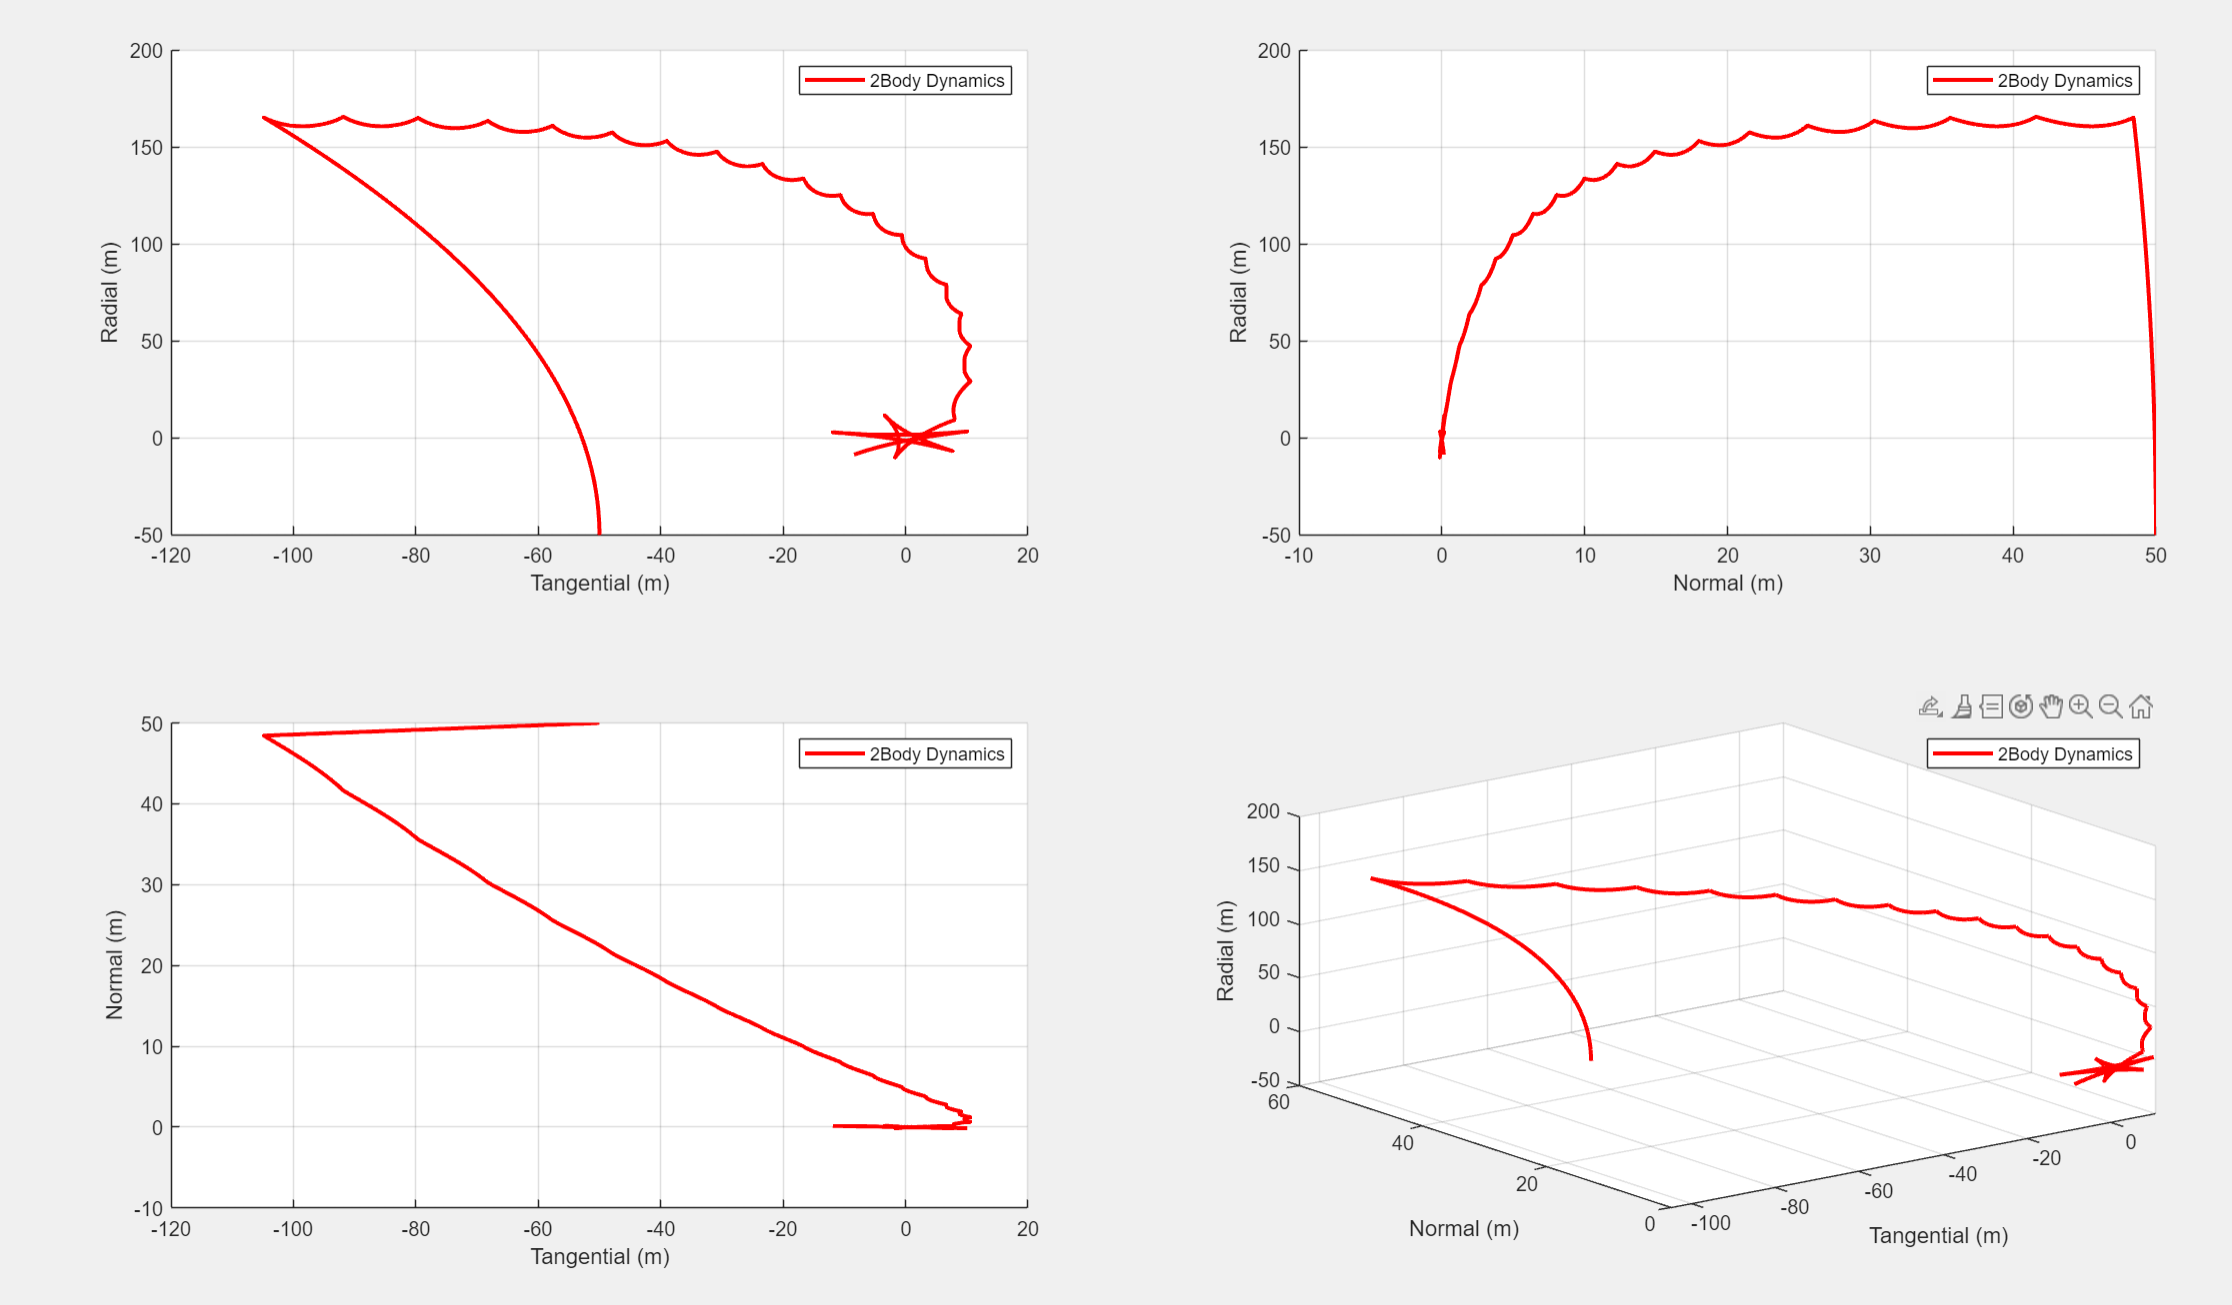
\includegraphics[width=0.7\textwidth]{PS5/Figures/position.png}
    \caption{RTN Trajectory}
    \label{fig:hcw_velocity}
\end{figure}

\begin{figure}[H]
    \centering
    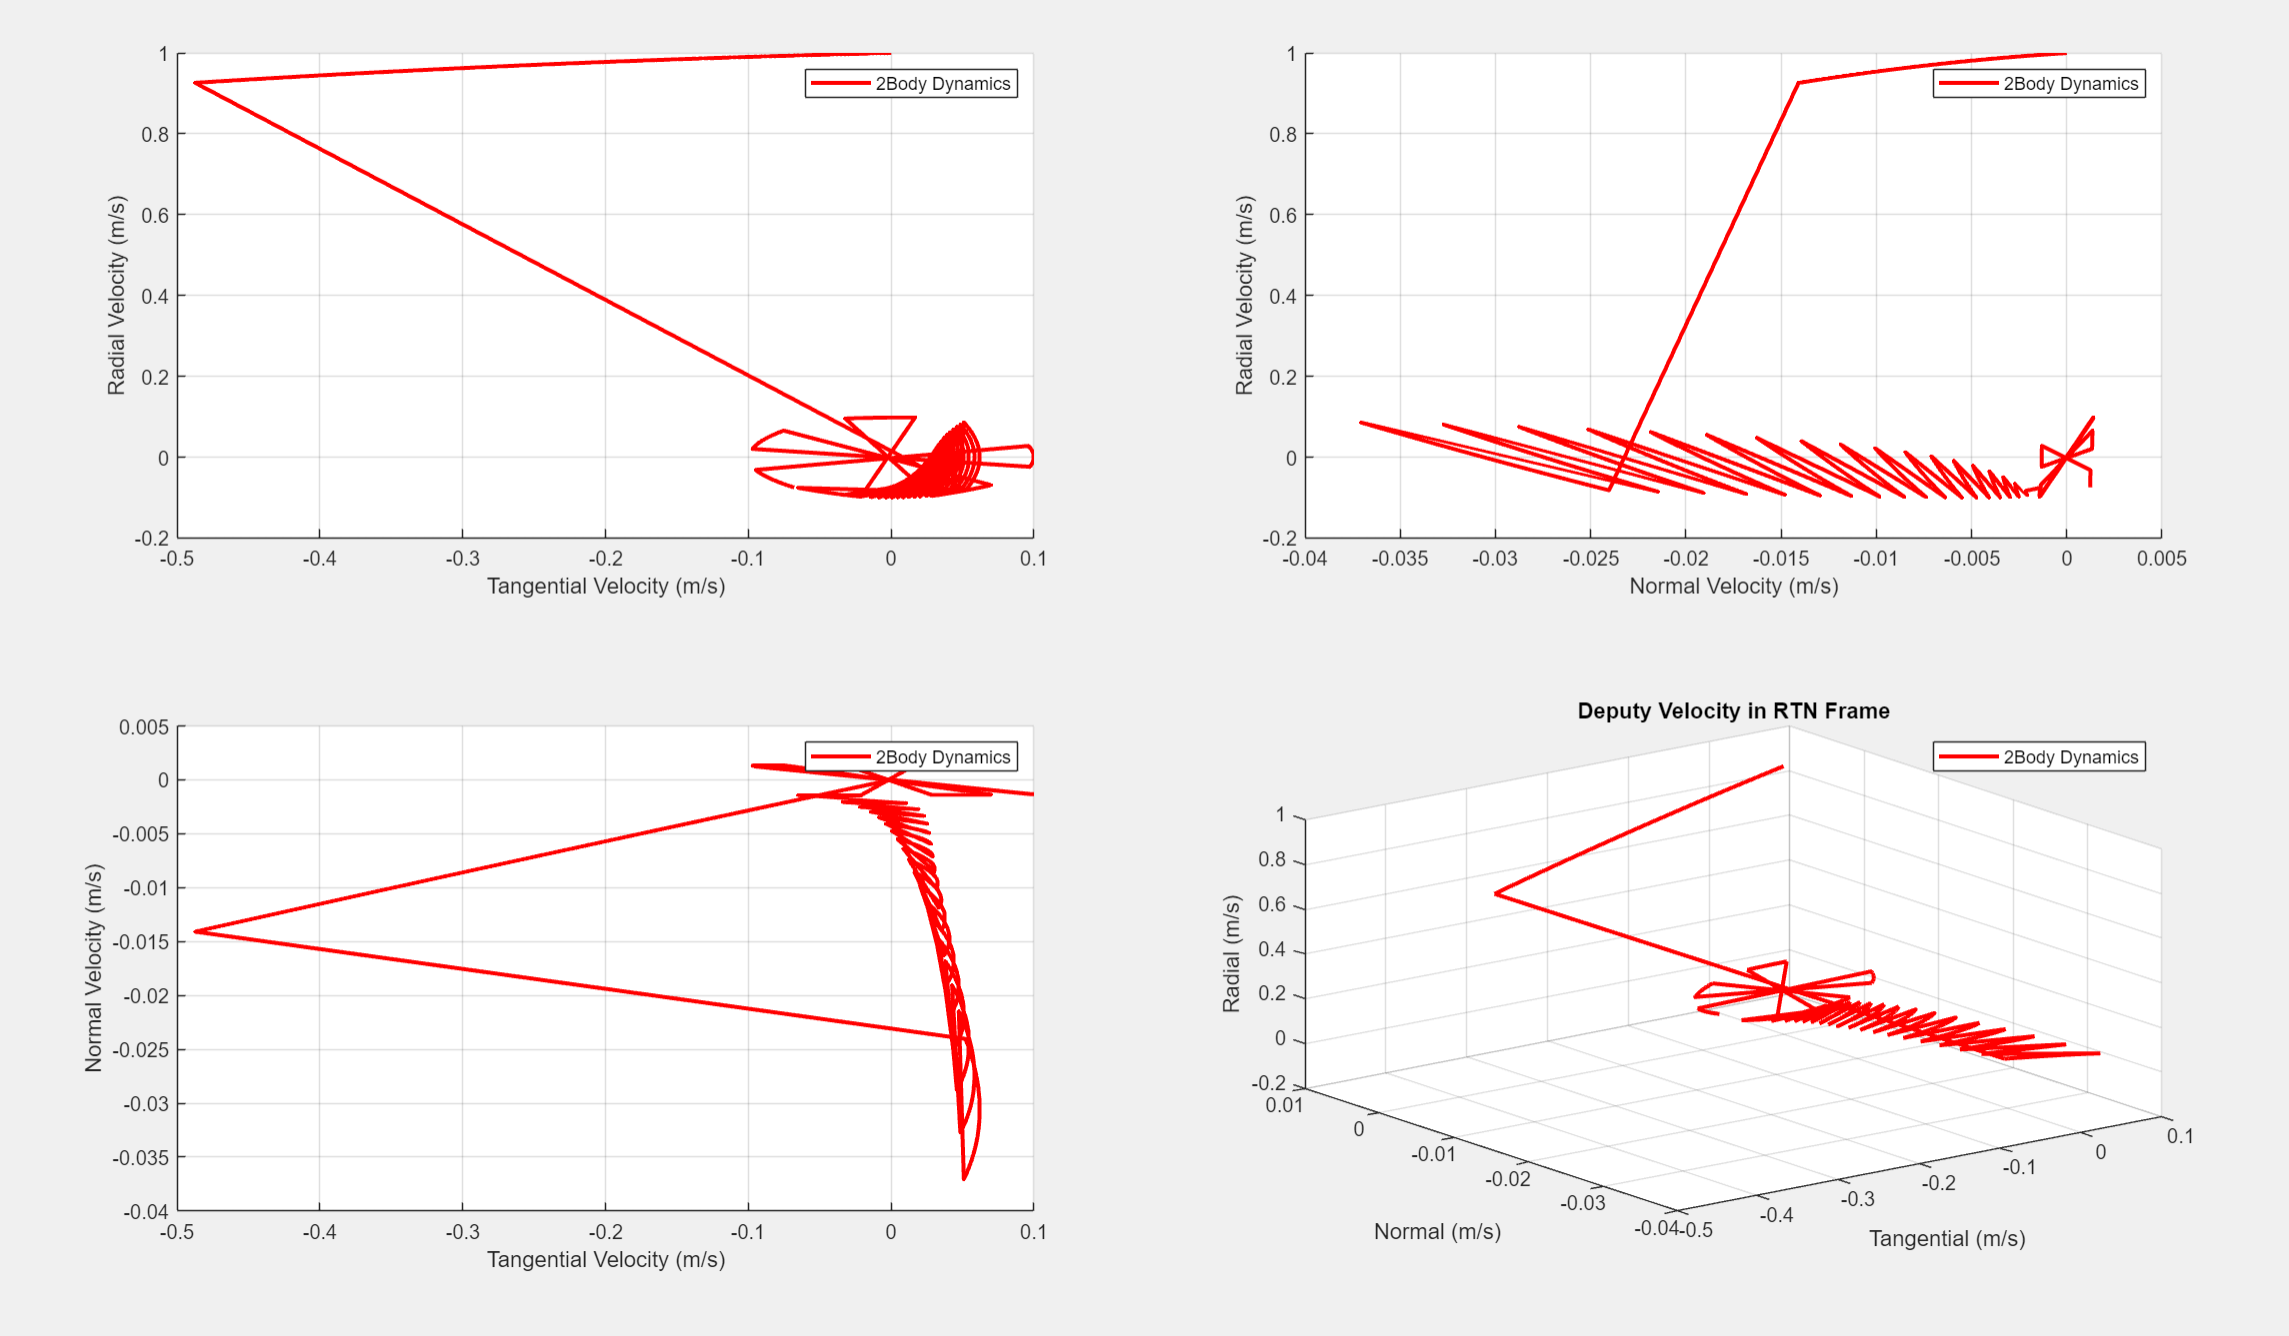
\includegraphics[width=0.7\textwidth]{PS5/Figures/velocity.png}
    \caption{RTN Velocity}
    \label{fig:hcw_velocity}
\end{figure}

\begin{figure}[H]
    \centering
    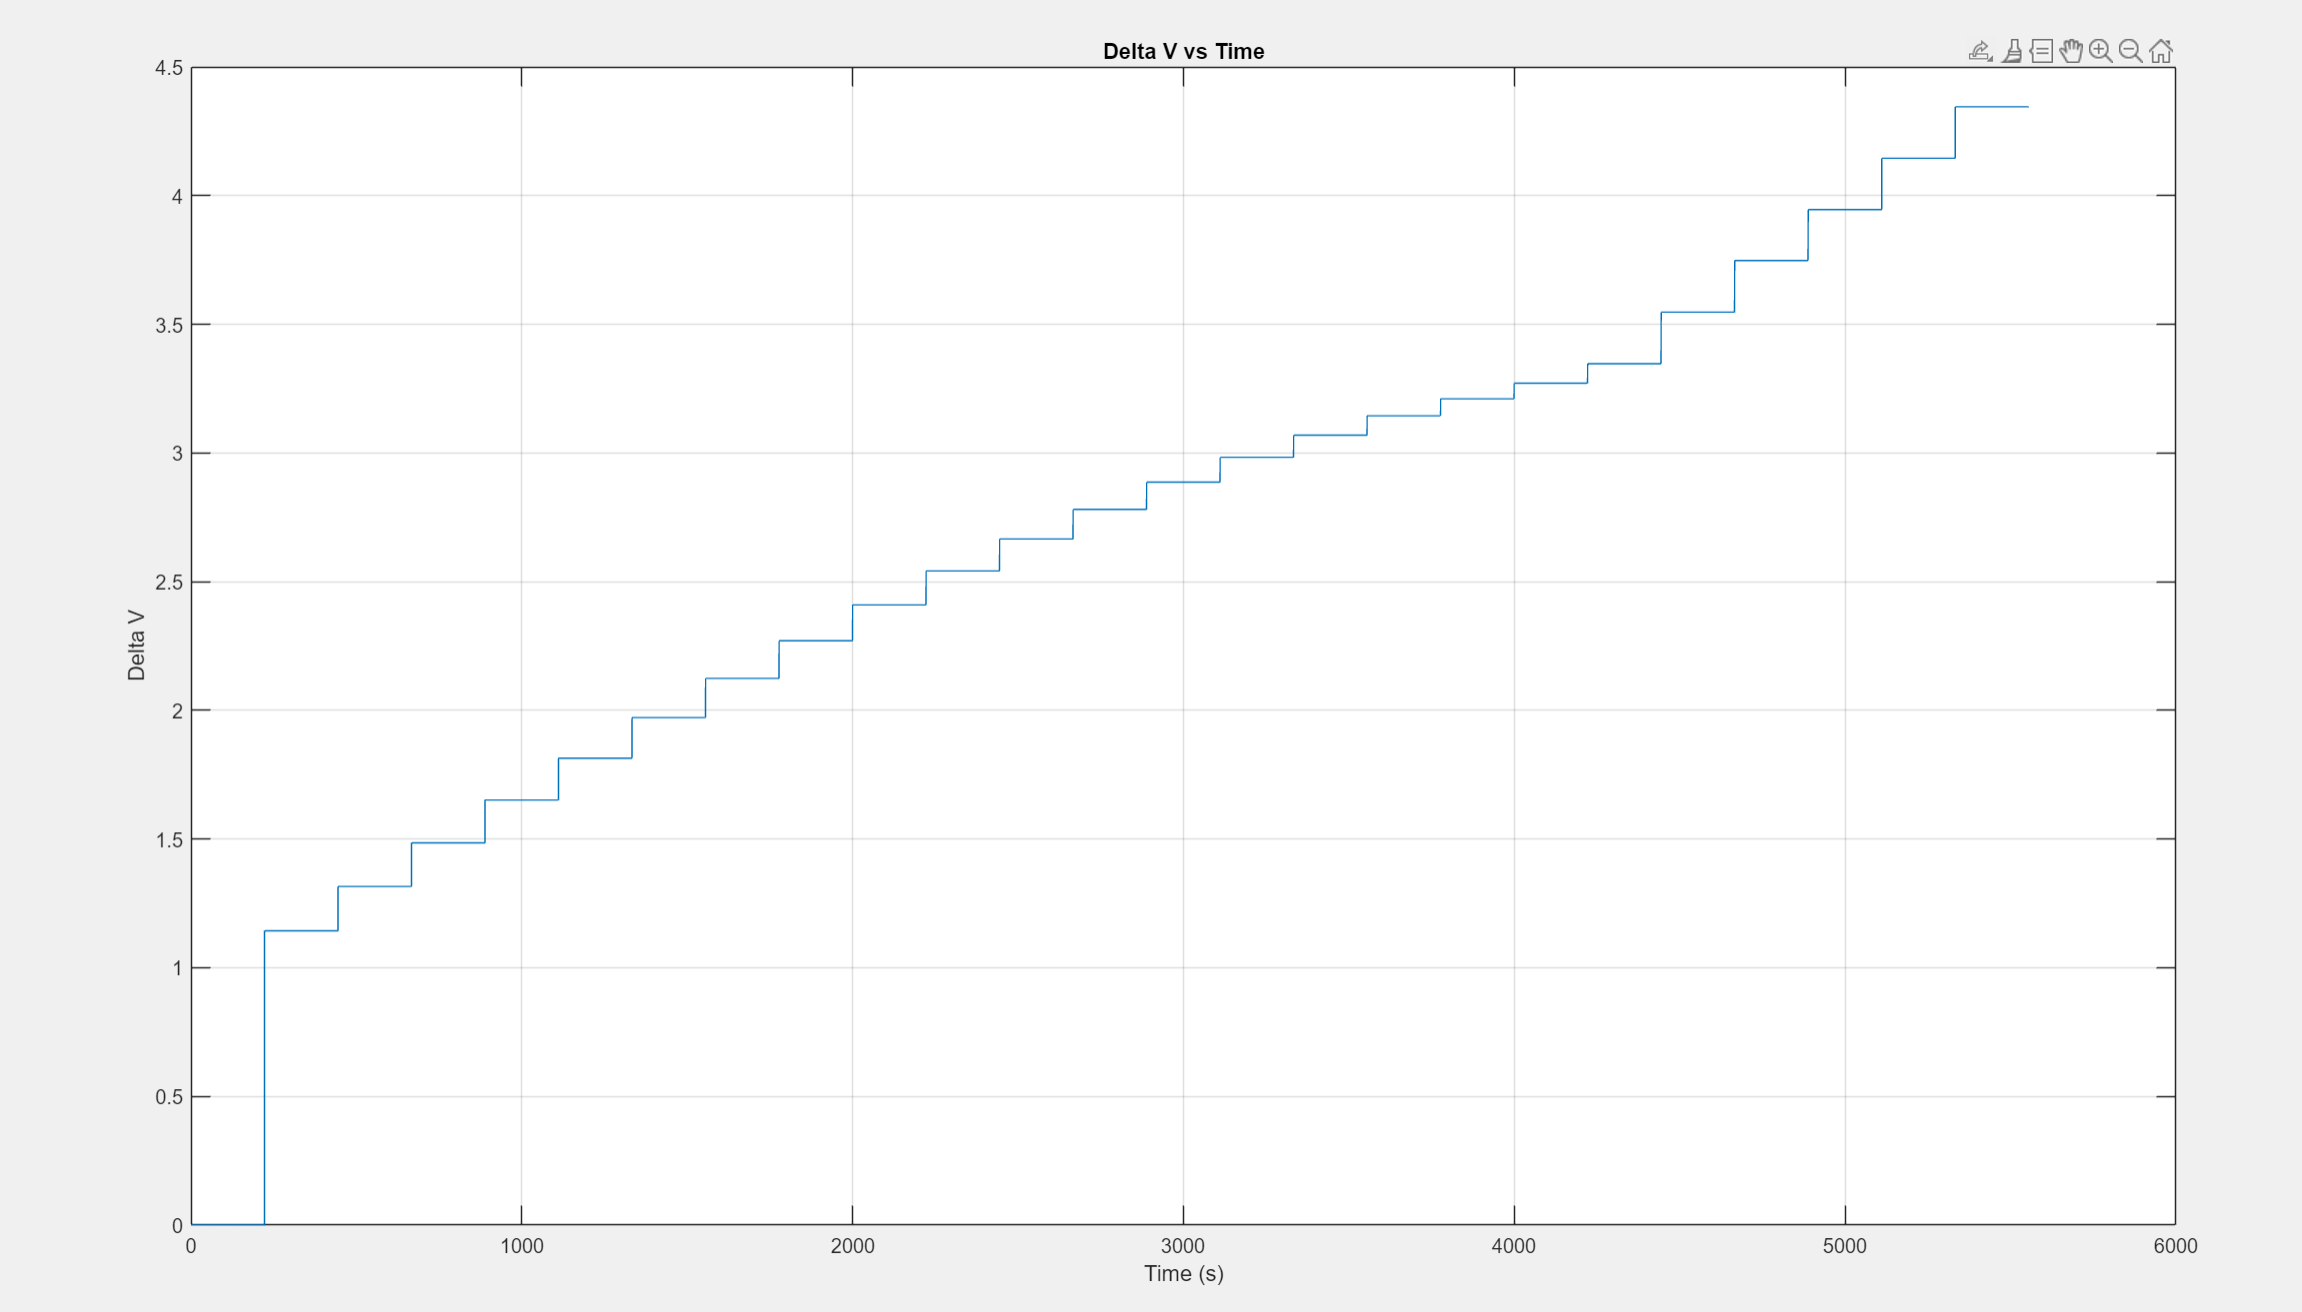
\includegraphics[width=0.7\textwidth]{PS5/Figures/dv.png}
    \caption{Dv usage over Time}
    \label{fig:hcw_velocity}
\end{figure}

As can be seen from the postion and velocity figures, the first burn is a significant one that cancels out most of the RTN velocity. From there, the algorithm proceeds in small steps to draw the spacecraft closer together, finally converging in a zone close to the chief.

The dv figure indicates a relatively low delta v of 4 m/s to converge a distance of 50m over the course of less than a third of an orbit.



\newpage
\section{Problem Set 6}

\subsection{Another Control Method}

We realized last week that our method of control from the previous pset was more continuous than impulsive, so we are flipping problem sets 5 and 6. Last weeks implementation is our continuous control (since we can shrink the time step between burns to be zero and thus have continuous thrust), and this week we implemented impulsive control.

For our impulse control this week, we decided to go with a solution to the HCW equations. Since we know where we want to be (docking to the target) we know we want to drive our RTN position to zero. Therefore, we know where we want to be, and if we know where we are, we can solve the HCW equations to determine the delta v we need to apply.

Since:
\begin{align}
r(t) = \Phi_{rr}r_0 + \Phi_{rv}v_0
\end{align}

We can set the final position to be zero (since we are docking) and rearrange to get
\begin{align}
v_0 = -\Phi_{rv}^{-1}\Phi_{rr}r
\end{align}

Thus, we can solve what the velocity needs to be after the maneuver, and if we know the starting RTN velocity we can calculate the delta v of the maneuver.

This methodology has several advantages. First, it can always take the position of the spacecraft and generate a necessary delta v to reach the target at a specified time frame. By decreasing the time frame, one can decrease delta v costs. However, it leaves the time frames (in terms of when to burn as well as how long the transfer will take) up to the user, which means there could be suboptimal solutions requested.

Below is the results of this methodology in our simulator. As you can see, from an arbitrary RTN starting state with arbitrary position and velocity, the solver is able to calculate the necessary trajectory and execute it to intercept the target spacecraft.


\begin{figure}[H]
    \centering
    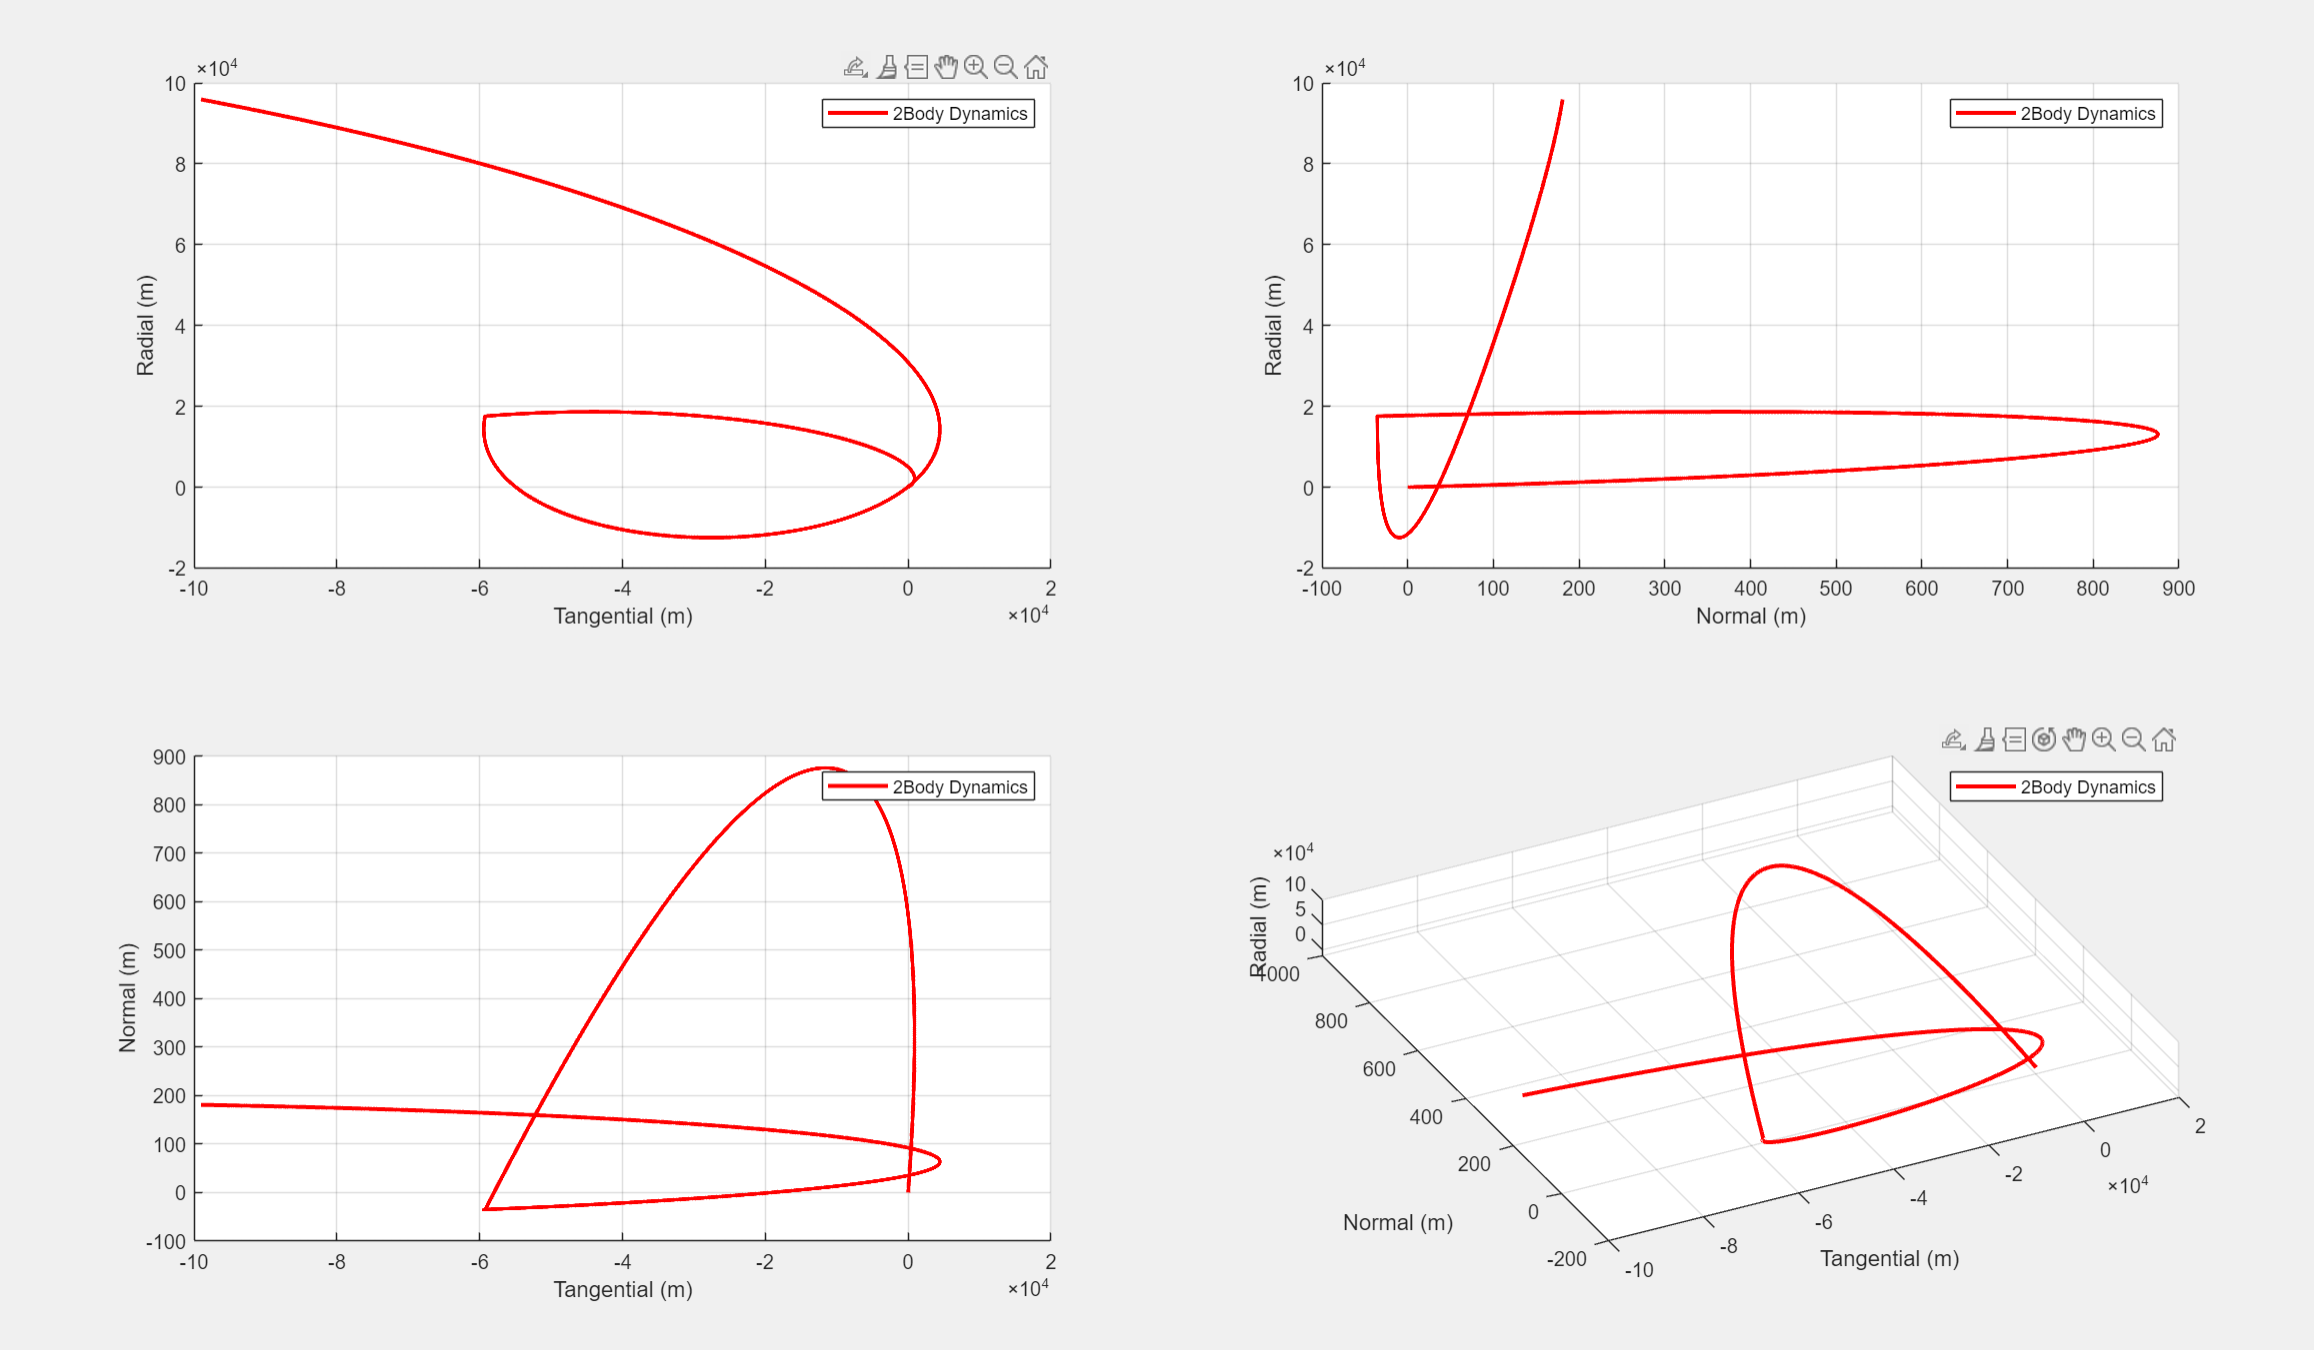
\includegraphics[width=0.7\textwidth]{PS6/Figures/trajectory.png}
    \caption{RTN Trajectory}
    \label{fig:hcw_velocity}
\end{figure}

\begin{figure}[H]
    \centering
    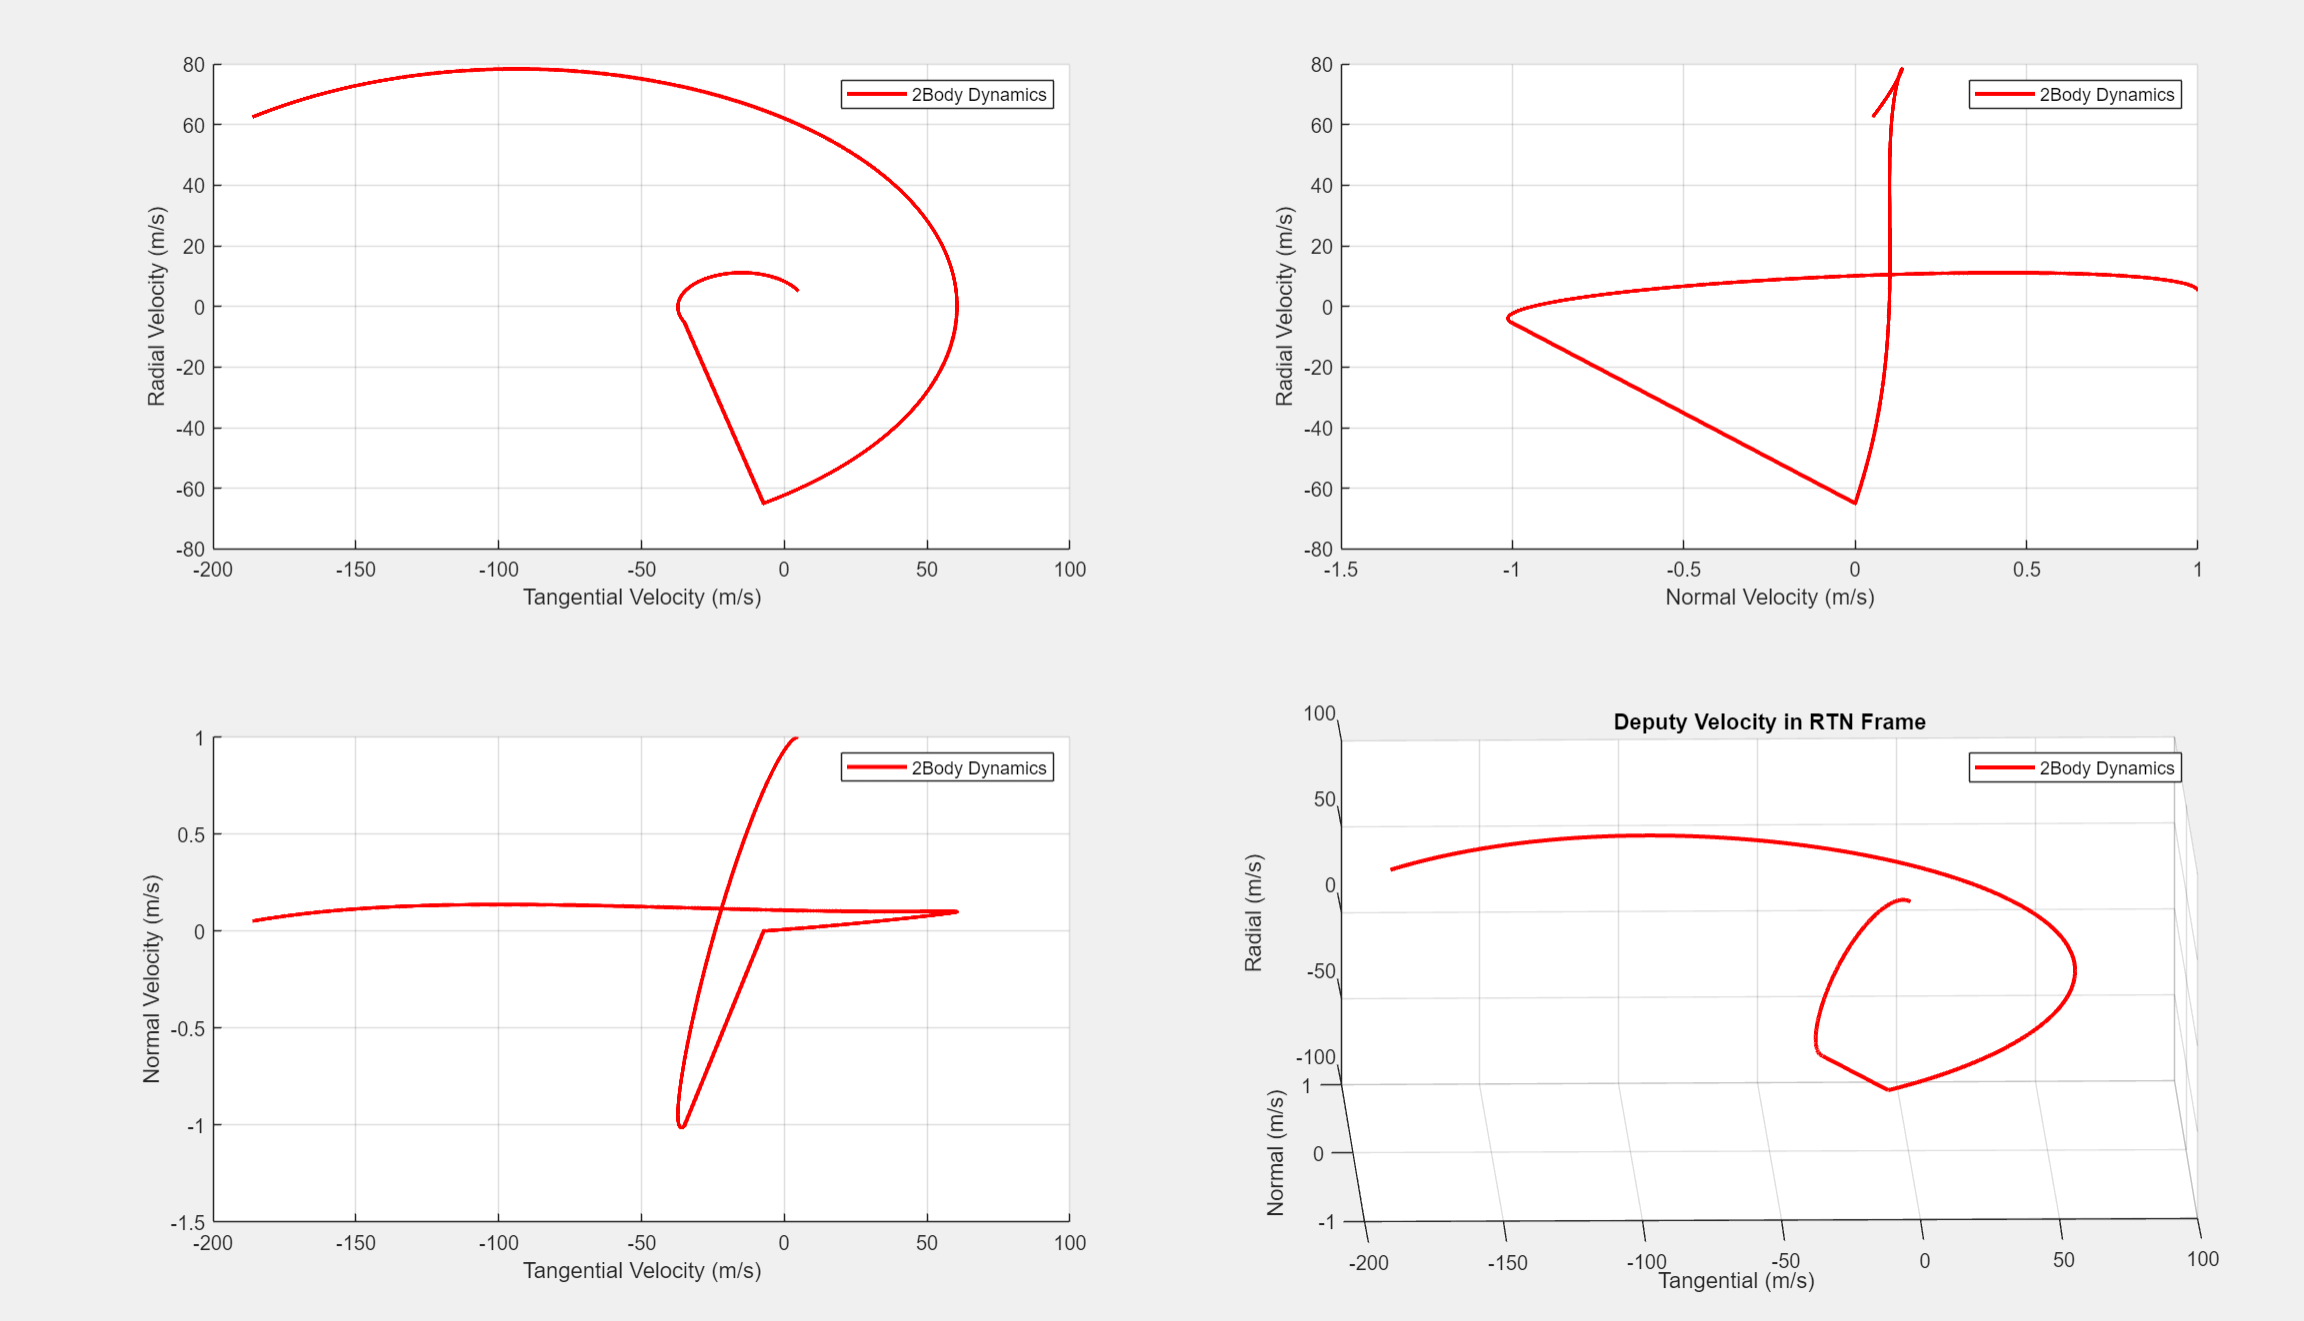
\includegraphics[width=0.7\textwidth]{PS6/Figures/velocity.png}
    \caption{RTN Velocity}
    \label{fig:hcw_velocity}
\end{figure}

We will not include a delta v plot over time for this problem, since it is rather simple - a single increase in delta v at one point in time.

Beyond the issues discussed above, this methodology has additional problems. First, it only works well in circular orbits due to it's reliance on HCW.

Our ground-truth simulation uses two-body dynamics for both spacecraft, implementing the impulsive maneuver as an instantaneous change in velocity at the calculated burn time. This implementation assumes perfect knowledge of the state vectors and perfect execution of the burn. In a real-world scenario, navigation errors and thruster imperfections would cause deviations from the planned trajectory.

This method also assumes small relative distances between spacecraft since the HCW equations are linearized around the reference orbit. For larger separations, the linear approximation breaks down and leads to targeting errors.

Unlike our continuous control approach from last week which required multiple small corrections, this impulsive method requires just a single, well-timed burn to achieve the desired rendezvous. While our continuous approach provides more robustness against disturbances and modeling errors by constantly adjusting the trajectory, this impulsive method is significantly more fuel-efficient for scenarios where the dynamics are well-known and external perturbations are minimal.

The single impulsive maneuver calculated by our algorithm approaches the theoretical minimum delta-v for a direct rendezvous transfer in circular orbits using HCW dynamics, making it particularly attractive for spacecraft with limited propellant budgets. However, this efficiency comes at the cost of flexibility and robustness that continuous control methods provide.

\newpage
\section{Problem Set 7}

\subsection{Finalizing Control Methods}

We have two control methods available to use in our simulation, one of which is a continuous method, the other of which is an impulsive method. As can be seen below, both are capable of driving a deputy spacecraft to the location of the chief:

\begin{figure}[H]
    \centering
    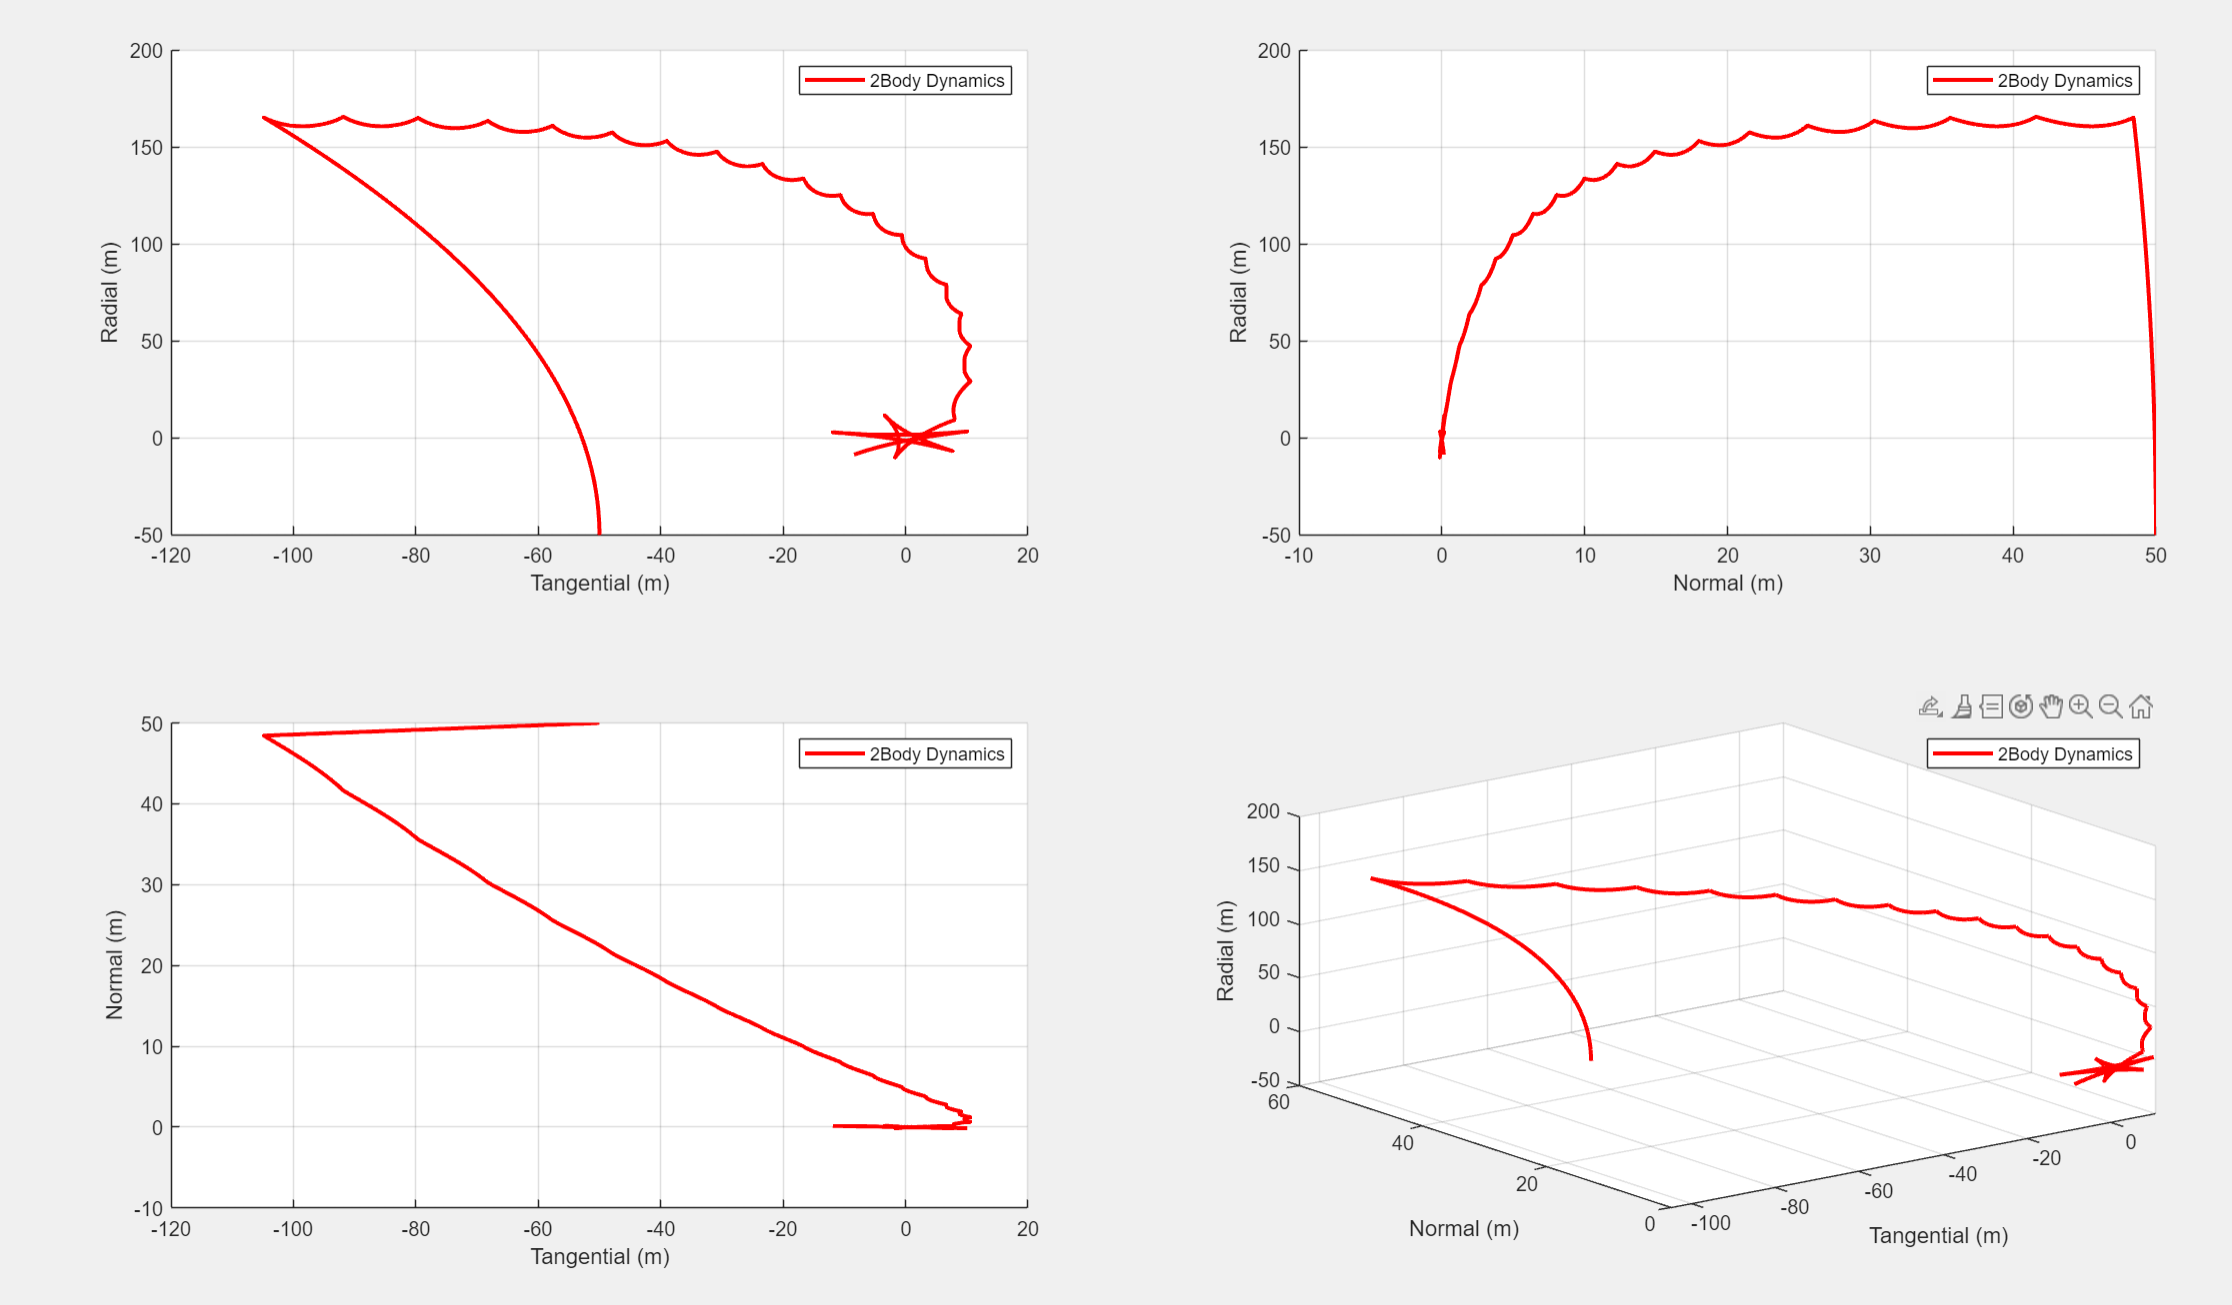
\includegraphics[width=0.7\textwidth]{PS7/Figures/position (1).png}
    \caption{Continuous Control Method}
    \label{fig:hcw_velocity}
\end{figure}

\begin{figure}[H]
    \centering
    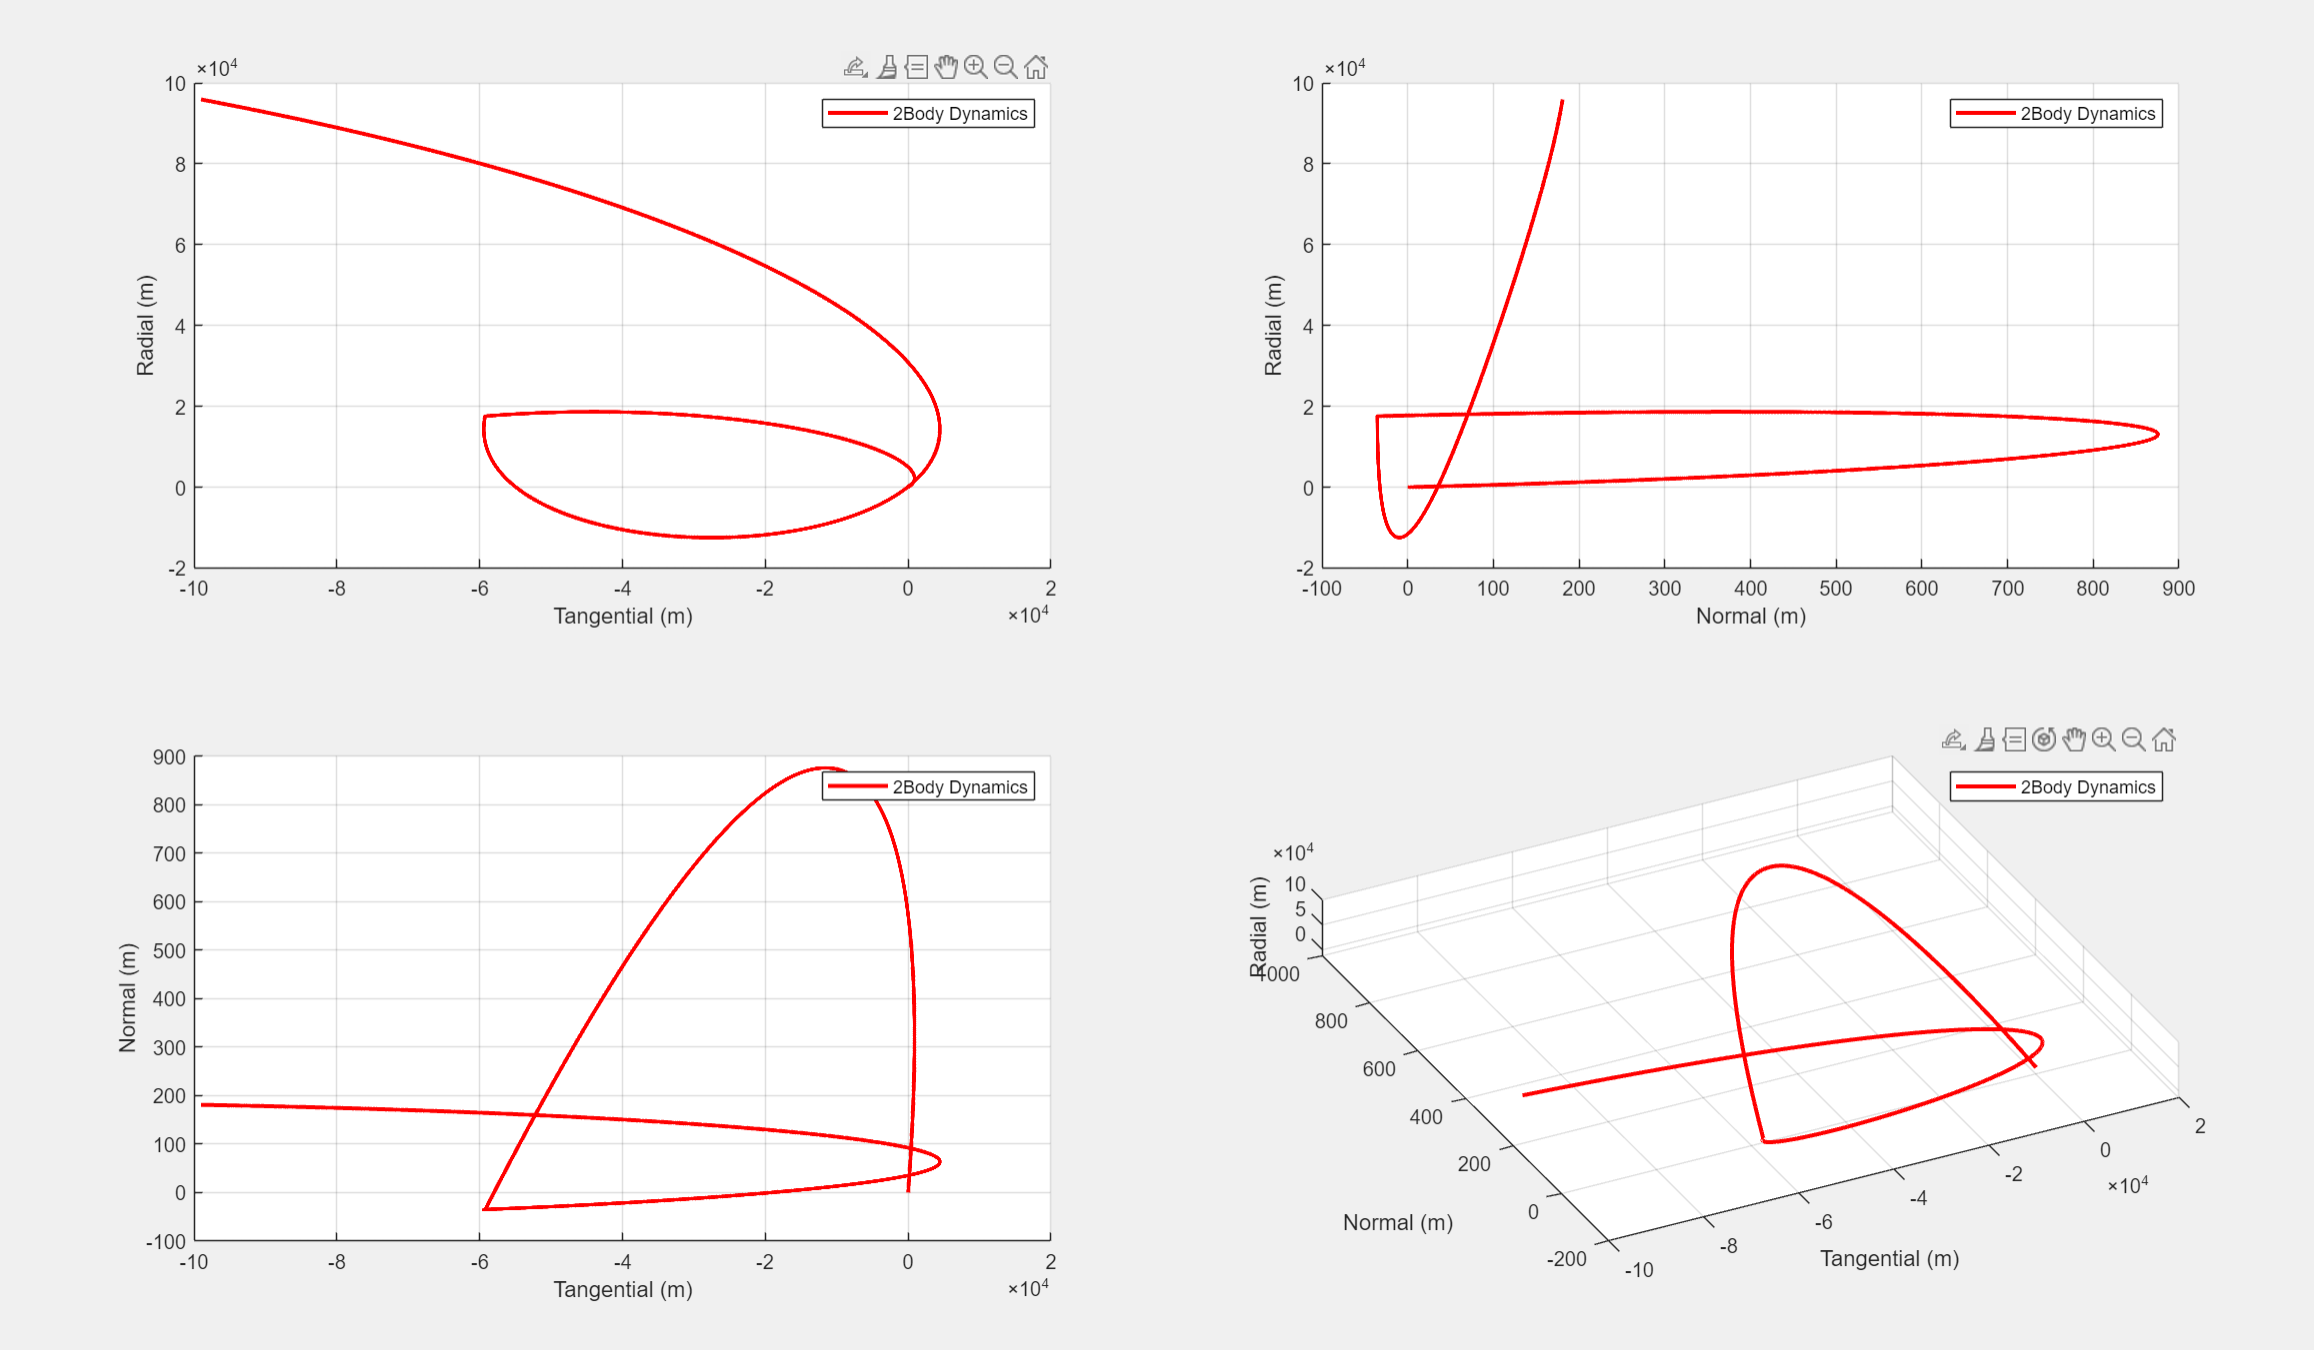
\includegraphics[width=0.7\textwidth]{PS7/Figures/trajectory (1).png}
    \caption{Impulsive Control Method}
    \label{fig:hcw_velocity}
\end{figure}

The continuous control methodology is made up of repeatedly canceling relative velocity and thrusting towards the target. The impulsive control method solves the HCW equations to determine the necessary delta v to impart to intercept the chief. There are pros and cons to each, with the main issues being that the continuous control ceases to converge once within a certain radius and is somewhat expensive, and the impulsive method relies on HCW assumptions, namely that the orbit is circular with no pertubations.


\subsection{Kick off Navigation System Design}

\subsubsection{Representation in Filter}
We worked on implementing an Extended Kalman Filter to estimate the state of the deputy. We used cartesian position and velocity (ECI) for the state representation inside the filter. Thus, we will be estimating the absolute state.

\subsubsection{Dynamics Model}
In line with our state representation in the filter, we decided to go with the absolute 2 body propagator with J2 effects for our dynamics model. While many of the other propogation methods we learned through this class may be faster, we have yet to encounter a computational bottleneck, so the 2 body propagator is a more accurate solution. To use this in our predict step, we linearize the dynamics about the current state by computing the derivative of each state element with respect to the others through central finite differencing of the dynamics, as is in the code below.

\begin{lstlisting}
function A = compute_linearized_dynamics(truth_state, simulation_settings)
    A = zeros(6, 6);
    for i=1:6
        state_plus = truth_state;
        state_minus = truth_state;

        h = 0.1;
        state_plus(i) = state_plus(i) + h;
        state_minus(i) = state_minus(i) - h;

        statedot_plus = dynamics.two_body_dynamics(0, state_plus, simulation_settings);
        statedot_minus = dynamics.two_body_dynamics(0, state_minus, simulation_settings);

        A(:,i) = ((statedot_plus - statedot_minus) / (2 * h));
    end
end
\end{lstlisting}

This becomes a matrix we can use to calculate the derivative of the state at the given state. It should be noted that we do the same thing for the control input matrix, where we represent our control input as a cartesian acceleration.

\subsubsection{Linearized Dynamics}
Once the state to state derivative matrix is calculated, we can call it A. With A, we need to find the state transition matrix F. To do this, we can multiply A by the timestep we use in the simulation, and add it to the identity matrix F = I + A*dt. The same procedure above is used to calculate the B matrix, where the dynamics are linearized about the current control input and state through central finite differencing, and then multiplied by the time step of the simulation. The resulting F and B matricies take the general forms below in the simulation:

\begin{figure}[H]
    \centering
    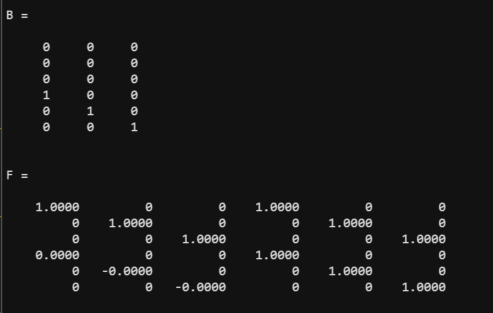
\includegraphics[width=0.7\textwidth]{PS7/Figures/Screenshot 2025-05-19 221625.png}
    \caption{State Transition Matrices}
    \label{fig:State Transition Matrices}
\end{figure}

These matrices make sense at a high level. First of all, since the state representation is cartesian position followed by cartesian velocity, it makes sense that in the F matrix, the position would be updated by the current state added to the time step (1 second) added to the current velocity. Additionally, since the orbit is not perfectly circular, it makes sense that the velocity in the F matrix is impacted mostly by the current velocity but also a bit by the spacecraft's position. The B matrix also makes sense, since the velocity is what will be first impacted by any cartesian accelerations (obtained by multiplying the accelerations by the current time step).

\subsubsection{Sensors}
For this first draft of the navigation, we decided to go with sensors that produce a range of 4 pseudo measurements - a range sensor that can detect cartesian position (based off of maybe some ground based radar or radio math), a range sensor that can detect cartesian velocity (again based on a ground based radar or something of that nature), a relative position sensor (maybe a camera on the chief) and a relative velocity sensor. To model these sensors, we inject gaussian noise into all of their measurements of the truth state.

\subsubsection{Measurement Model}
Given these measurements, we can create a measurement model H that can map the current state to the expected measurements. Given the pseudo measurements discussed above, this H matrix is fairly trivial, as it takes the form of 2 combined identity matrices:

\begin{figure}[H]
    \centering
    \includegraphics[width=0.7\textwidth]{PS7/Figures/Screenshot 2025-05-19 224040.png}
    \caption{H Matrix}
    \label{fig:H Matrix}
\end{figure}


\subsubsection{Sensitivity Matrix}

\begin{lstlisting}
% Predict Step
A = our_algorithms.compute_linearized_dynamics(truth_state, simulation_settings);
B = our_algorithms.compute_linearized_control(truth_state);
F = eye(6) +  A * dt;
keyboard
x_0 = F * truth_state;
P_0 = F * P * F' + Q;

% Update Step
z = H * x_0;
y = measurement - z;
K = P_0 * H' * inv((H * P_0 * H') + R);
x_1 = x_0 + K * y;
P_1 = (eye(6) - (K * H)) * P_0;
\end{lstlisting}

\begin{figure}[H]
    \centering
    \includegraphics[width=0.7\textwidth]{PS7/Figures/Screenshot 2025-05-20 143614.png}
    \caption{Sensitivity Matrix}
    \label{fig:Sensitivity Matrix}
\end{figure}

\newpage
\section{Problem Set 8}

\subsection{Finalizing Navigation Methods}

We implemented our Kalman filter after completing the set-up work from last week. For our ground truth, we used the 2 body propagator with J2 effects that we developed early in the course. We then corrupted the ground truth with guassian noise (of zero mean and reasonable standard deviation) to simulate sensor measurements for the spacecraft. As discussed last week, we include 4 methods of sensing - relative position and velocity, and absolute position and velocity.

Our initial state estimate is set to the initial position of the simulation, while our initial covariance is set to the identity matrix. Similarly, we initially set Q and R to be identity matrices as well, and then tuned them to get reasonable filter results.

Our filter ended up working very well. In the graphs below, we plot the truth state from the 2 body propogator, next to the estimated state from the kalman filter. The additional plots describe the error and quality of the filter. The code for the filter lives in the appendix.

\begin{figure}[H]
    \centering
    \includegraphics[width=0.7\textwidth]{PS8/Figures/position.png}
    \caption{Estimated Position}
    \label{fig:hcw_velocity}
\end{figure}

\begin{figure}[H]
    \centering
    \includegraphics[width=0.7\textwidth]{PS8/Figures/velocity.png}
    \caption{Estimated Velocity}
    \label{fig:hcw_velocity}
\end{figure}

\begin{figure}[H]
    \centering
    \includegraphics[width=0.7\textwidth]{PS8/Figures/error.png}
    \caption{Error in Estimate}
    \label{fig:hcw_velocity}
\end{figure}
%%%%%%%%%%%%%%%%%%%%%%%%%%%%%%%
% REFERENCES
%%%%%%%%%%%%%%%%%%%%%%%%%%%%%%%
\newpage
\section{References}
\printbibliography[heading=none]

%%%%%%%%%%%%%%%%%%%%%%%%%%%%%%%
% APPENDIX 1: CODE
%%%%%%%%%%%%%%%%%%%%%%%%%%%%%%%
\newpage
\appendix
\section{Appendix: Code}

% Optional: Git repository link to your code
% All code for this project can be found in the following \href{}{Git repository}.

\subsection{Problem Set 1 Code}

\textbf{constants.m}
\begin{lstlisting}
classdef constants
    properties( Constant = true )
         mu = 3.986004 * 10^14 % m^3/s^2
         earth_radius = 6378000 % m
         J2 = 1.08263 * 10^(-3)
    end
 end
\end{lstlisting}

\textbf{dynamics.m}
\begin{lstlisting}
function statedot = dynamics(t, state, simulation_settings)
% Take in state vector and return statedot vector (accelerations)
r = state(1:3);
v = state(4:6);

a = -constants.mu * r / (norm(r) ^ 3);

if simulation_settings.J2
    a_j2_x = 1.5 * constants.J2 * constants.mu * (constants.earth_radius ^ 2 / norm(r) ^ 5) * (1 - (5 * (r(3) / norm(r)) ^ 2)) * r(1);
    a_j2_y = 1.5 * constants.J2 * constants.mu * (constants.earth_radius ^ 2 / norm(r) ^ 5) * (1 - (5 * (r(3) / norm(r)) ^ 2)) * r(2);
    a_j2_z = 1.5 * constants.J2 * constants.mu * (constants.earth_radius ^ 2 / norm(r) ^ 5) * (3 - (5 * (r(3) / norm(r)) ^ 2)) * r(3);
    a_j2 = [a_j2_x; a_j2_y; a_j2_z];
    a = a + a_j2;
end

r_dot = v;
v_dot = a;

statedot = [r_dot; v_dot];

end
\end{lstlisting}

\textbf{plotter.m}
\begin{lstlisting}
function plotter(result, graphics_settings)
    if graphics_settings.orbit_eci
        plot_orbit_eci(result)
    end

    if graphics_settings.compare_numerical_vs_kepler
        compare_numerical_vs_kepler(result)
    end

    if graphics_settings.plot_orbital_elements.base_elems
        plot_orbital_elements(result, graphics_settings)
    end

    if graphics_settings.plot_eccentricity_vector
        plot_eccentricity_vector(result)
    end

    if graphics_settings.plot_ang_momentum_vector
        plot_ang_momentum_vector(result)
    end

    if graphics_settings.plot_specific_energy
        plot_specific_energy(result)
    end
end

function compare_numerical_vs_kepler(result)
    t = result.t_num;
    state_history_num = result.state_history_num;
    t_span = result.t_kep;
    state_history_kep = result.state_history_kep;

    state_history_kep = interp1(t_span, state_history_kep, t, 'linear');

    error_rtn = zeros(size(state_history_kep));
    for j = 1:size(state_history_kep, 1)
        error_rtn(j, :) = util.ECI2RTN(state_history_kep(j, :)) - util.ECI2RTN(state_history_num(j, :));
    end
    
    figure;
    hold on;
    plot(t, error_rtn)
    xlabel('Time (s)');
    ylabel('Absolute Error (m and m/s)');
    title('Absolute Error vs Time, RTN Frame');
    legend('Error R_r', 'Error R_t', 'Error R_n', 'Error V_r', 'Error V_t', 'Error V_n');

end

function plot_orbit_eci(result)
    state_history = result.state_history_num;

    % Extract positions
    x = state_history(:, 1);
    y = state_history(:, 2);
    z = state_history(:, 3);

    % Show Earth
    [xe, ye, ze] = sphere(50);
    xe = constants.earth_radius * xe;
    ye = constants.earth_radius * ye;
    ze = constants.earth_radius * ze;

    figure;

    % Plot Earth
    surf(xe, ye, ze, 'FaceColor', 'blue', 'EdgeColor', 'none');
    hold on;

    % Plot Orbit
    plot3(x, y, z, 'c-', 'LineWidth', 2); 
    grid on;
    xlabel('X');
    ylabel('Y');
    zlabel('Z');
    title('ECI Trajectory');
    view(3);
    axis equal;
end

function plot_orbital_elements(result, graphics_settings)
    t = result.t_num;
    oe_history = result.oe_history;

    a     = oe_history(:, 1);
    e     = oe_history(:, 2);
    i     = oe_history(:, 3);
    RAAN  = oe_history(:, 4);  
    omega = oe_history(:, 5);
    nu    = oe_history(:, 6);  

    if graphics_settings.plot_orbital_elements.J2_mean_analytical_solution
        J2_analytical = zeros(length(result.state_history_num), 2);
        for j = 1:length(result.state_history_num)
            K = -(3 * constants.J2 * sqrt(constants.mu) * constants.earth_radius^2) / (2 * ((1 - e(j)^2)^2) * (a(j) ^ (7/2)));
            RAAN_j2 = result.initial_conditions(4) - (K * t(j) * cos(i(j)));
            w_j2 = result.initial_conditions(5) + ((K / 2) * t(j) * ((5 * (cos(i(j)) ^ 2)) - 1));
            J2_analytical(j, :) = [RAAN_j2, w_j2];
        end
    end

    figure;
    tiledlayout(3,2, 'Padding', 'compact', 'TileSpacing', 'compact');

    nexttile;
    plot(t, a, 'r'); grid on;
    xlabel('Time'); ylabel('a (km)');
    title('Semi-Major Axis');

    nexttile;
    plot(t, e, 'g'); grid on;
    xlabel('Time'); ylabel('e');
    title('Eccentricity');

    nexttile;
    plot(t, rad2deg(i), 'y'); grid on;
    xlabel('Time'); ylabel('Inclination (deg)');
    title('Inclination');

    nexttile;
    hold on;
    plot(t, rad2deg(RAAN), 'm'); grid on;
    if graphics_settings.plot_orbital_elements.J2_mean_analytical_solution
        plot(t, rad2deg(J2_analytical(:,1)), 'k');
        legend('Numerical', 'J2 Mean Analytical');
    end
    xlabel('Time'); ylabel('RAAN (deg)');
    title('RAAN');

    nexttile;
    hold on;
    plot(t, rad2deg(omega), 'c'); grid on;
    if graphics_settings.plot_orbital_elements.J2_mean_analytical_solution
        plot(t, rad2deg(J2_analytical(:,2)), 'k');
        legend('Numerical', 'J2 Mean Analytical');
    end
    xlabel('Time'); ylabel('\omega (deg)');
    title('Argument of Periapsis');
    

    nexttile;
    plot(t, rad2deg(nu), 'k'); grid on;
    xlabel('Time'); ylabel('\nu (deg)');
    title('True Anomaly');
end

function plot_eccentricity_vector(result)
    figure;
    hold on
    plot(result.t_num, result.ecc_vector_history(:,1), 'r'); 
    plot(result.t_num, result.ecc_vector_history(:,2), 'g');
    plot(result.t_num, result.ecc_vector_history(:,3), 'b');
    grid on;
    xlabel('Time (s)'); ylabel('Eccentricity Vector');
    title('Eccentricity Vector over Time');
    legend('X_comp', 'Y_comp', 'Z_comp');
end

function plot_ang_momentum_vector(result)
    figure;
    hold on
    plot(result.t_num, result.ang_mom_history(:,1), 'r'); 
    plot(result.t_num, result.ang_mom_history(:,2), 'g');
    plot(result.t_num, result.ang_mom_history(:,3), 'b');
    grid on;
    xlabel('Time (s)'); ylabel('Angular Momentum Vector');
    title('Angular Momentum Vector over Time');
    legend('X_comp', 'Y_comp', 'Z_comp');
end

function plot_specific_energy(result)
    figure;
    hold on
    plot(result.t_num, result.energy_history, 'b'); 
    grid on;
    xlabel('Time (s)'); ylabel('Specific Energy (J)');
    title('Specific Energy over Time');
end
\end{lstlisting}

\textbf{sim\_config.m}
\begin{lstlisting}
% Input initial conditions in orbital elments. Units of meters and degrees
initial_conditions = [10000000, 0.1, 45, 0, 0, 0]; % OEs

% Input time span of simulation in start:time_step:end format. Units of seconds
time_span = 0:1:500000;

% Simulation settings
simulation_settings.numerical_propogation = true;
simulation_settings.keplerian_propogation = false;
simulation_settings.J2 = true;

% Set graphics settings for graph output
graphics_settings.orbit_eci = true;
graphics_settings.compare_numerical_vs_kepler = false;

graphics_settings.plot_orbital_elements = struct();
graphics_settings.plot_orbital_elements.base_elems = true;
graphics_settings.plot_orbital_elements.J2_mean_analytical_solution = false;

graphics_settings.plot_eccentricity_vector = false;
graphics_settings.plot_ang_momentum_vector = false;
graphics_settings.plot_specific_energy = false;


sim = simulator(initial_conditions, time_span, simulation_settings, graphics_settings);
sim.run_simulator();
\end{lstlisting}

\textbf{simulator.m}
\begin{lstlisting}
classdef simulator
    properties
        initial_conditions
        time_span
        simulation_settings
        graphics_settings
    end

    methods
        function self = simulator(initial_conditions, time_span, simulation_settings, graphics_settings)
            self.initial_conditions = initial_conditions;
            self.time_span = time_span;
            self.simulation_settings = simulation_settings;
            self.graphics_settings = graphics_settings;
        end

        function run_simulator(self)
            a = self.initial_conditions(1);
            e = self.initial_conditions(2);
            i = deg2rad(self.initial_conditions(3));
            RAAN = deg2rad(self.initial_conditions(4));
            w = deg2rad(self.initial_conditions(5));
            v = deg2rad(self.initial_conditions(6));
            result.initial_conditions = self.initial_conditions;

            if self.simulation_settings.numerical_propogation
                initial_state = util.OE2ECI(a, e, i, RAAN, w, v);

                % Perform Simulation
                options = odeset('RelTol', 1e-7, 'AbsTol', 1e-9);
                [t, state_history_num] = ode45(@(t, state_history_num) dynamics(t, state_history_num, self.simulation_settings), [0 self.time_span(end)], initial_state, options);
                result.state_history_num = state_history_num;
                result.t_num = t;

                % Gather orbital element history and other interesting information
                oe_history = zeros(length(state_history_num), 6);
                ecc_vector_history = zeros(length(state_history_num), 3);
                ang_mom_history = zeros(length(state_history_num), 3);
                energy_history = zeros(length(state_history_num), 1);
                for j = 1:length(state_history_num)
                    oe_history(j, :) = util.ECI2OE(state_history_num(j, :));
                    ecc_vector_history(j, :) = util.get_ecc_vector(state_history_num(j, :));
                    ang_mom_history(j, :) = util.get_ang_momentum(state_history_num(j, :));
                    energy_history(j, :) = util.get_energy(state_history_num(j, :));
                end
                result.oe_history = oe_history;
                result.ecc_vector_history = ecc_vector_history;
                result.ang_mom_history = ang_mom_history;
                result.energy_history = energy_history;
            end

            if self.simulation_settings.keplerian_propogation
                n = sqrt(constants.mu / a ^ 3);
                dt = self.time_span(2) - self.time_span(1);
                state_history_kep = zeros(length(self.time_span), 6);
                for j=1:length(self.time_span)
                    state_kep = util.OE2ECI(a, e, i, RAAN, w, v);
                    state_history_kep(j,:) = state_kep';
                    E = 2 * atan2(tan(v/2) * sqrt((1 - e) / (1 + e)), 1);
                    M = E - e*sin(E);
                    M_new = M + (n * dt);
                    E_new = util.MtoE(M_new, e, 10^(-6));
                    v_new = 2 * atan2(sqrt((1 + e) / (1 - e)) * tan(E_new / 2), 1);
                    v = v_new;
                end
                result.state_history_kep = state_history_kep;
                result.t_kep = self.time_span;
            end
            plotter(result, self.graphics_settings)
        end
    end
end
\end{lstlisting}

\textbf{util.m}
\begin{lstlisting}
classdef util
    methods (Static)
        function state_eci = OE2ECI(a, e, i, RAAN, w, v)
            p = a * (1 - e^2);
            r = p / (1 + e*cos(v));
            rPQW = [r*cos(v); r*sin(v); 0];
            vPQW = [sqrt(constants.mu/p) * -sin(v); sqrt(constants.mu/p)*(e + cos(v)); 0];
        
            R1 = [cos(-RAAN) sin(-RAAN) 0;...
                -sin(-RAAN) cos(-RAAN) 0;...
                0       0       1];
            R2 = [1  0        0;...
                0  cos(-i) sin(-i);...
                0 -sin(-i) cos(-i)];
            R3 = [cos(-w) sin(-w) 0;...
                -sin(-w) cos(-w) 0;...
                0        0        1]; R = R1 * R2 * R3;
        
            rECI = R * rPQW;
            vECI = R * vPQW;
            state_eci = [rECI; vECI];
        end

        function H = get_ang_momentum(state)
            R = state(1:3);
            V = state(4:6);
            H = cross(R, V);
        end

        function E = get_ecc_vector(state)
            R = state(1:3);
            V = state(4:6);
            H = util.get_ang_momentum(state);
            mu = constants.mu;
            E = (cross(V,H)/mu)-(R/norm(R));
        end

        function E = get_energy(state)
            oes = util.ECI2OE(state);
            a = oes(1);
            E = -constants.mu / (2 * a);
        end

        function OEs = ECI2OE(state)
            mu = constants.mu;
            R = state(1:3);
            V = state(4:6);
            r = norm(R);
            
            %Get to Perifocal
            H = util.get_ang_momentum(state);
            h = norm(H);
            E = util.get_ecc_vector(state);
            e = norm(E);
            p = (h)^2/mu;
            a = p / (1 - e^2);
            n = sqrt(mu/a^3);
            E = atan2((dot(R, V)/(n*a^2)), (1-(r/a)));
            v = 2 * atan(sqrt((1+e)/(1-e)) * tan(E/2));
            
            %Find Angles
            W = [H(1)/h H(2)/h H(3)/h];
            i = atan2(sqrt(W(1)^2 + W(2)^2), W(3));
            RAAN = atan2(W(1), -W(2));
            w = atan2((R(3)/sin(i)), R(1)*cos(RAAN)+R(2)*sin(RAAN)) - v;
            if rad2deg(w) > 180
                w = w - 2*pi;
            end
            
            OEs = [a, e, i, RAAN, w, v];
        end

        function state_pqw = OE2PQW(a, e, i, RAAN, w, v)
            p = a * (1 - e^2);
            r = p / (1 + e*cos*(v));
            P = r*cos(v);
            Q = r*sin(v);
            W = 0;
            rPQW = [P; Q; W];
            vPQW = sqrt(constants.mu / p) * [-sin(v); e + cos(v); 0];
            state_pqw = [rPQW; vPQW];
        end

        function E = MtoE(M, e, err)
            E = M; N = 0;
            delta = (E - e*sin(E) - M) / (1 - e*cos(E));
            while (delta > err || N < 100)
                delta = (E - e*sin(E) - M) / (1 - e*cos(E));
                E = E - delta;
                N = N + 1;
            end
        end

        function state_rtn = ECI2RTN(state_eci)
            r_eci = state_eci(1:3)';
            v_eci = state_eci(4:6)';
            n = cross(r_eci, v_eci);

            R = r_eci / norm(r_eci);
            N = n / norm(n);
            T = cross(N, R);

            R_eci2rtn = [R, T, N];

            r_rtn = R_eci2rtn * r_eci;

            f_dot = norm(cross(r_eci, v_eci)) / norm(r_eci)^2;
            w = [0,0,f_dot]';
            v_rtn = (R_eci2rtn * v_eci) - cross(w, r_rtn);

            state_rtn = [r_rtn; v_rtn];
        end
    end
 end
\end{lstlisting}
\subsection{Problem Set 2 Code}

\textbf{constants.m}
\begin{lstlisting}
classdef constants
    properties( Constant = true )
         mu = 3.986004 * 10^14 % m^3/s^2
         earth_radius = 6378000 % m
         J2 = 1.08263 * 10^(-3)
    end
 end
\end{lstlisting}

\textbf{dynamics.m}
\begin{lstlisting}
classdef dynamics
    methods (Static)
        function statedot = two_body_dynamics(t, state, simulation_settings)
            % Take in state vector and return statedot vector (accelerations)
            r = state(1:3);
            v = state(4:6);

            a = -constants.mu * r / (norm(r) ^ 3);

            if simulation_settings.J2
                a_j2_x = 1.5 * constants.J2 * constants.mu * (constants.earth_radius ^ 2 / norm(r) ^ 5) * (1 - (5 * (r(3) / norm(r)) ^ 2)) * r(1);
                a_j2_y = 1.5 * constants.J2 * constants.mu * (constants.earth_radius ^ 2 / norm(r) ^ 5) * (1 - (5 * (r(3) / norm(r)) ^ 2)) * r(2);
                a_j2_z = 1.5 * constants.J2 * constants.mu * (constants.earth_radius ^ 2 / norm(r) ^ 5) * (3 - (5 * (r(3) / norm(r)) ^ 2)) * r(3);
                a_j2 = [a_j2_x; a_j2_y; a_j2_z];
                a = a + a_j2;
            end

            r_dot = v;
            v_dot = a;

            statedot = [r_dot; v_dot];
        end

        function statedot = dynamics_with_relative(t, state, simulation_settings)
            % State input is relative state in rtn, followed by chief state in eci
            rho = state(1:3);
            drho = state(4:6);
            chief_state_rtn = util.ECI2RTN(state(7:12), state(7:12));
            r_0 = [norm(state(7:9)); 0; 0];
            v_0 = chief_state_rtn(4:6);

            h = norm(cross(r_0, v_0));
            omega = h / norm(r_0)^2;
            omega_dot = -2 * h * v_0(1) / (norm(r_0) ^ 3);
        
            k = -constants.mu / ((norm(r_0) + rho(1))^2 + rho(2)^2 + rho(3)^2)^(3/2);
            xddot = k * (norm(r_0) + rho(1)) + (constants.mu / norm(r_0)^2) + (2 * omega * drho(2)) + (omega_dot * rho(2)) + (rho(1) * omega^2);
            yddot = (k * rho(2)) - (2 * omega * drho(1)) - (omega_dot * rho(1)) + (rho(2) * omega^2);
            zddot = k * rho(3);

            ddrho = [xddot; yddot; zddot];

            chief_dot = dynamics.two_body_dynamics(t, state(7:12), simulation_settings);
            
            statedot = [drho; ddrho; chief_dot];
        end
    end
end
\end{lstlisting}

\textbf{sim\_config.m}
\begin{lstlisting}
clear all;
close all;
clc;

% Input initial conditions in orbital elments. Units of meters and degrees
initial_conditions_chief = [6780000, 0.0006, 51.6, 0, 0, 0]; % OEs
initial_conditions_chief = [6780000, 0, 0, 0, 0, 0]; 

% Time step and number of orbits
num_orbits = 3;
time_step = 1;

% Simulation settings
simulation_settings.numerical_propogation = true;
simulation_settings.keplerian_propogation = false;
simulation_settings.J2 = false;
simulation_settings.relative_deputy = true;
simulation_settings.absolute_deputy = true;

% Set graphics settings
graphics_settings.orbit_eci = false;
graphics_settings.compare_numerical_vs_kepler = false;
graphics_settings.plot_relative_position_deputy = true;
graphics_settings.plot_relative_position_deputy_comparison = true;
graphics_settings.plot_relative_position_error = true;
graphics_settings.plot_orbital_elements = struct();
graphics_settings.plot_orbital_elements.base_elems = false;
graphics_settings.plot_orbital_elements.J2_mean_analytical_solution = false;
graphics_settings.plot_eccentricity_vector = false;
graphics_settings.plot_ang_momentum_vector = false;
graphics_settings.plot_specific_energy = false;

% Case 1: Equal semi-major axis
disp('Running Case 1: Equal semi-major axis');
initial_conditions_deputy = [0; 0; 0; 1; 1; 0]; % Position and velocity relative to chief in RTN
sim1 = simulator(initial_conditions_chief, initial_conditions_deputy, num_orbits, time_step, simulation_settings, graphics_settings);
sim1.run_simulator();

% Case 2: Non-zero difference in semi-major axis
disp('Running Case 2: Non-zero difference in semi-major axis');
initial_conditions_deputy_case2 = [0; 0; 0; 10; 1; 0]; % Added 10 m/s in radial direction
sim2 = simulator(initial_conditions_chief, initial_conditions_deputy_case2, num_orbits, time_step, simulation_settings, graphics_settings);
sim2.run_simulator();

% Case 3: Calculate and apply maneuver to eliminate drift
disp('Running Case 3: Calculating and applying maneuver to bound motion');
simulation_settings.calculate_maneuver = true;
simulation_settings.apply_maneuver = true;
graphics_settings.plot_maneuver_comparison = true;
sim3 = simulator(initial_conditions_chief, initial_conditions_deputy_case2, num_orbits, time_step, simulation_settings, graphics_settings);
sim3.run_simulator();
\end{lstlisting}

\textbf{simulator.m}
\begin{lstlisting}
classdef simulator
    properties
        initial_conditions
        initial_conditions_deputy
        time_span
        dt
        simulation_settings
        graphics_settings
    end

    methods
        function self = simulator(initial_conditions_chief, initial_conditions_deputy, num_orbits, time_step, simulation_settings, graphics_settings)
            self.initial_conditions = initial_conditions_chief;
            self.initial_conditions_deputy = initial_conditions_deputy;
            time = (num_orbits * (2*pi*sqrt(self.initial_conditions(1)^3 / constants.mu)));
            time_span = 0:time_step:time;
            self.dt = time_step;
            self.time_span = time_span;
            self.simulation_settings = simulation_settings;
            self.graphics_settings = graphics_settings;
        end

        function run_simulator(self)
            a = self.initial_conditions(1);
            e = self.initial_conditions(2);
            i = deg2rad(self.initial_conditions(3));
            RAAN = deg2rad(self.initial_conditions(4));
            w = deg2rad(self.initial_conditions(5));
            v = deg2rad(self.initial_conditions(6));
            result.initial_conditions = self.initial_conditions;
            result.dt = self.dt;

            if self.simulation_settings.numerical_propogation
                initial_state_eci = util.OE2ECI(a, e, i, RAAN, w, v);

                % Perform Simulation
                options = odeset('RelTol', 1e-12, 'AbsTol', 1e-12);
                if self.simulation_settings.relative_deputy
                    initial_state = [self.initial_conditions_deputy; initial_state_eci];
                    [t, state_history] = ode45(@(t, state_history) dynamics.dynamics_with_relative(t, state_history, self.simulation_settings), self.time_span, initial_state, options);
                    result.state_history_num = state_history(:, 7:12);
                    result.relative_state_history = state_history(:, 1:6);
                    result.t_num = t;
                else
                    [t, state_history_num] = ode45(@(t, state_history_num) dynamics.two_body_dynamics(t, state_history_num, self.simulation_settings), self.time_span, initial_state_eci, options);
                    result.state_history_num = state_history_num;
                    result.t_num = t;
                end

                % Implementation for part (2c) - compute deputy orbit from chief orbit
                if self.simulation_settings.absolute_deputy
                    % Create initial state for deputy by applying variations to chief
                    % Convert relative state in RTN to ECI
                    rho_RTN = self.initial_conditions_deputy(1:3);
                    drho_RTN = self.initial_conditions_deputy(4:6);
                    
                    % Calculate RTN basis vectors directly
                    r_chief = initial_state_eci(1:3);
                    v_chief = initial_state_eci(4:6);
                    
                    R_hat = r_chief / norm(r_chief);
                    h_vec = cross(r_chief, v_chief);
                    N_hat = h_vec / norm(h_vec);
                    T_hat = cross(N_hat, R_hat);
                    
                    % RTN to ECI transformation matrix (each column is a basis vector)
                    R_rtn2eci = [R_hat, T_hat, N_hat];
                    
                    % Calculate deputy position in ECI
                    r_deputy_eci = r_chief + R_rtn2eci * rho_RTN;
                    
                    % Calculate angular velocity of RTN frame
                    omega = norm(h_vec) / (norm(r_chief)^2);
                    omega_vec = omega * N_hat;
                    
                    % Calculate deputy velocity in ECI
                    v_deputy_eci = v_chief + R_rtn2eci * drho_RTN + cross(omega_vec, R_rtn2eci * rho_RTN);
                    
                    % Combine to get deputy initial state in ECI
                    deputy_initial_state_eci = [r_deputy_eci; v_deputy_eci];
                    
                    % Propagate deputy orbit using the existing two_body_dynamics
                    [t_deputy, state_history_deputy] = ode45(@(t, state) dynamics.two_body_dynamics(t, state, self.simulation_settings), self.time_span, deputy_initial_state_eci, options);
                    
                    % Transform deputy orbit to RTN frame relative to chief
                    deputy_in_rtn = zeros(length(t), 6);
                    for j = 1:length(t)
                        % Get chief state at this time point
                        r_chief_j = result.state_history_num(j, 1:3)';
                        v_chief_j = result.state_history_num(j, 4:6)';
                        
                        % Calculate RTN basis vectors
                        R_hat_j = r_chief_j / norm(r_chief_j);
                        h_vec_j = cross(r_chief_j, v_chief_j);
                        N_hat_j = h_vec_j / norm(h_vec_j);
                        T_hat_j = cross(N_hat_j, R_hat_j);
                        
                        % ECI to RTN transformation matrix
                        R_eci2rtn_j = [R_hat_j, T_hat_j, N_hat_j]';
                        
                        % Deputy position and velocity in ECI
                        r_deputy_j = state_history_deputy(j, 1:3)';
                        v_deputy_j = state_history_deputy(j, 4:6)';
                        
                        % Calculate relative position in RTN
                        rho_j = R_eci2rtn_j * (r_deputy_j - r_chief_j);
                        
                        % Calculate relative velocity in RTN
                        omega_j = norm(h_vec_j) / (norm(r_chief_j)^2);
                        omega_vec_j = omega_j * N_hat_j;
                        drho_j = R_eci2rtn_j * (v_deputy_j - v_chief_j - cross(omega_vec_j, r_deputy_j - r_chief_j));
                        
                        deputy_in_rtn(j, :) = [rho_j; drho_j]';
                    end
                    
                    result.deputy_state_history = state_history_deputy;
                    result.deputy_in_rtn = deputy_in_rtn;
                    result.t_deputy = t_deputy;
                    
                    % Part (2e) and (2f) - Calculate and apply maneuver if requested
                    if isfield(self.simulation_settings, 'calculate_maneuver') && self.simulation_settings.calculate_maneuver
                        % Calculate the optimal maneuver to correct the drift
                        [delta_v, optimal_time_index, maneuver_point] = self.calculate_drift_correction(result.deputy_state_history, result.state_history_num, result.t_num);
                        
                        % Save maneuver information
                        result.maneuver_time = result.t_num(optimal_time_index);
                        result.maneuver_delta_v = delta_v;
                        result.maneuver_time_index = optimal_time_index;
                        result.maneuver_point = maneuver_point;
                        
                        % Apply maneuver if requested
                        if isfield(self.simulation_settings, 'apply_maneuver') && self.simulation_settings.apply_maneuver
                            % Get the state at maneuver point
                            maneuver_state = result.deputy_state_history(optimal_time_index, :);
                            
                            % Calculate the new velocity after maneuver
                            v_deputy = maneuver_state(4:6);
                            v_unit = v_deputy / norm(v_deputy);
                            
                            % We need to match chief's semi-major axis
                            a_chief = util.ECI2OE(result.state_history_num(optimal_time_index, :));
                            a_chief = a_chief(1);
                            r_deputy = norm(maneuver_state(1:3));
                            
                            % Calculate required velocity magnitude for the desired orbit
                            v_new_mag = sqrt(constants.mu * (2/r_deputy - 1/a_chief));
                            v_new = v_unit * v_new_mag;
                            
                            % Apply the maneuver post_maneuver_state = maneuver_state;
                            post_maneuver_state(4:6) = v_new;
                            
                            % Continue propagation from maneuver point
                            t_remaining = self.time_span(self.time_span > result.t_num(optimal_time_index));
                            if ~isempty(t_remaining)
                                [t_post, state_post] = ode45(@(t, state) dynamics.two_body_dynamics(t, state, self.simulation_settings), t_remaining, post_maneuver_state, options);
                                
                                % Store post-maneuver trajectory
                                t_combined = [result.t_num(1:optimal_time_index); t_post];
                                deputy_combined = [result.deputy_state_history(1:optimal_time_index, :); state_post];
                                
                                % Transform post-maneuver trajectory to RTN
                                deputy_rtn_post = zeros(length(t_post), 6);
                                for j = 1:length(t_post)
                                    % Find closest chief state time
                                    [~, t_idx] = min(abs(result.t_num - t_post(j)));
                                    
                                    % Chief state
                                    r_chief_j = result.state_history_num(t_idx, 1:3)';
                                    v_chief_j = result.state_history_num(t_idx, 4:6)';
                                    
                                    % Calculate RTN basis
                                    R_hat_j = r_chief_j / norm(r_chief_j);
                                    h_vec_j = cross(r_chief_j, v_chief_j);
                                    N_hat_j = h_vec_j / norm(h_vec_j);
                                    T_hat_j = cross(N_hat_j, R_hat_j);
                                    
                                    R_eci2rtn_j = [R_hat_j, T_hat_j, N_hat_j]';
                                    
                                    % Deputy state
                                    r_deputy_j = state_post(j, 1:3)';
                                    v_deputy_j = state_post(j, 4:6)';
                                    
                                    % Calculate relative position
                                    rho_j = R_eci2rtn_j * (r_deputy_j - r_chief_j);
                                    
                                    % Calculate relative velocity
                                    omega_j = norm(h_vec_j) / (norm(r_chief_j)^2);
                                    omega_vec_j = omega_j * N_hat_j;
                                    drho_j = R_eci2rtn_j * (v_deputy_j - v_chief_j - cross(omega_vec_j, r_deputy_j - r_chief_j));
                                    
                                    deputy_rtn_post(j, :) = [rho_j; drho_j]';
                                end
                                
                                % Combine trajectories
                                deputy_rtn_combined = [result.deputy_in_rtn(1:optimal_time_index, :); deputy_rtn_post];
                                
                                % Save combined results
                                result.t_combined = t_combined;
                                result.deputy_state_combined = deputy_combined;
                                result.deputy_in_rtn_combined = deputy_rtn_combined;
                            end
                        end
                    end
                end

                % Gather orbital element history and other interesting information
                oe_history = zeros(length(result.state_history_num), 6);
                ecc_vector_history = zeros(length(result.state_history_num), 3);
                ang_mom_history = zeros(length(result.state_history_num), 3);
                energy_history = zeros(length(result.state_history_num), 1);
                for j = 1:length(result.state_history_num)
                    oe_history(j, :) = util.ECI2OE(result.state_history_num(j, :));
                    ecc_vector_history(j, :) = util.get_ecc_vector(result.state_history_num(j, :));
                    ang_mom_history(j, :) = util.get_ang_momentum(result.state_history_num(j, :));
                    energy_history(j, :) = util.get_energy(result.state_history_num(j, :));
                end
                result.oe_history = oe_history;
                result.ecc_vector_history = ecc_vector_history;
                result.ang_mom_history = ang_mom_history;
                result.energy_history = energy_history;
            end

            if self.simulation_settings.keplerian_propogation
                n = sqrt(constants.mu / a ^ 3);
                state_history_kep = zeros(length(self.time_span), 6);
                for j=1:length(self.time_span)
                    state_kep = util.OE2ECI(a, e, i, RAAN, w, v);
                    state_history_kep(j,:) = state_kep';
                    E = 2 * atan2(tan(v/2) * sqrt((1 - e) / (1 + e)), 1);
                    M = E - e*sin(E);
                    M_new = M + (n * self.dt);
                    E_new = util.MtoE(M_new, e, 10^(-9));
                    v_new = 2 * atan2(sqrt((1 + e) / (1 - e)) * tan(E_new / 2), 1);
                    v = v_new;
                end
                result.state_history_kep = state_history_kep;
                result.t_kep = self.time_span;
            end
            plotter(result, self.graphics_settings);
        end
        
        function [delta_v, optimal_time_index, maneuver_point] = calculate_drift_correction(self, deputy_state_history, chief_state_history, t)
            % Calculate orbital elements for both satellites
            deputy_oe = zeros(length(t), 6);
            chief_oe = zeros(length(t), 6);
            
            for i = 1:length(t)
                deputy_oe(i, :) = util.ECI2OE(deputy_state_history(i, :));
                chief_oe(i, :) = util.ECI2OE(chief_state_history(i, :));
            end
            
            % Calculate semi-major axis difference
            delta_a = deputy_oe(:, 1) - chief_oe(:, 1);
            disp(['Current semi-major axis difference: ', num2str(delta_a(end)), ' meters']);
            
            % Find points of minimum and maximum radius (approximate apogee/perigee)
            deputy_radius = zeros(length(t), 1);
            for i = 1:length(t)
                deputy_radius(i) = norm(deputy_state_history(i, 1:3));
            end
            
            [~, min_r_idx] = min(deputy_radius);
            [~, max_r_idx] = max(deputy_radius);
            
            % Calculate velocities at these points
            v_min_r = norm(deputy_state_history(min_r_idx, 4:6));
            v_max_r = norm(deputy_state_history(max_r_idx, 4:6));
            
            % Calculate required velocities for bounded motion
            a_target = chief_oe(1, 1); % Target semi-major axis = chief's
            r_min = deputy_radius(min_r_idx);
            r_max = deputy_radius(max_r_idx);
            
            v_req_min_r = sqrt(constants.mu * (2/r_min - 1/a_target));
            v_req_max_r = sqrt(constants.mu * (2/r_max - 1/a_target));
            
            % Calculate delta-v at both locations
            dv_min_r = abs(v_req_min_r - v_min_r);
            dv_max_r = abs(v_req_max_r - v_max_r);
            
            % Choose the more efficient maneuver
            if dv_min_r <= dv_max_r
                delta_v = dv_min_r;
                optimal_time_index = min_r_idx;
                maneuver_point = [r_min, t(min_r_idx)];
                disp(['Optimal maneuver at minimum radius (perigee), delta-v = ', num2str(delta_v), ' m/s']);
            else
                delta_v = dv_max_r;
                optimal_time_index = max_r_idx;
                maneuver_point = [r_max, t(max_r_idx)];
                disp(['Optimal maneuver at maximum radius (apogee), delta-v = ', num2str(delta_v), ' m/s']);
            end
        end
    end
end
\end{lstlisting}

\textbf{util.m}
\begin{lstlisting}
classdef util
    methods (Static)
        function state_eci = OE2ECI(a, e, i, RAAN, w, v)
            p = a * (1 - e^2);
            r = p / (1 + e*cos(v));
            rPQW = [r*cos(v); r*sin(v); 0];
            vPQW = [sqrt(constants.mu/p) * -sin(v); sqrt(constants.mu/p)*(e + cos(v)); 0];
        
            R1 = [cos(-RAAN) sin(-RAAN) 0;...
                -sin(-RAAN) cos(-RAAN) 0;...
                0       0       1];
            R2 = [1  0        0;...
                0  cos(-i) sin(-i);...
                0 -sin(-i) cos(-i)];
            R3 = [cos(-w) sin(-w) 0;...
                -sin(-w) cos(-w) 0;...
                0        0        1];
            R = R1 * R2 * R3;
        
            rECI = R * rPQW;
            vECI = R * vPQW;
            state_eci = [rECI; vECI];
        end

        function H = get_ang_momentum(state)
            R = state(1:3);
            V = state(4:6);
            H = cross(R, V);
        end

        function E = get_ecc_vector(state)
            R = state(1:3);
            V = state(4:6);
            H = util.get_ang_momentum(state);
            mu = constants.mu;
            E = (cross(V,H)/mu)-(R/norm(R));
        end

        function E = get_energy(state)
            oes = util.ECI2OE(state);
            a = oes(1);
            E = -constants.mu / (2 * a);
        end

        function OEs = ECI2OE(state)
            mu = constants.mu;
            R = state(1:3);
            V = state(4:6);
            r = norm(R);
            
            %Get to Perifocal
            H = util.get_ang_momentum(state);
            h = norm(H);
            E = util.get_ecc_vector(state);
            e = norm(E);
            p = (h)^2/mu;
            a = p / (1 - e^2);
            n = sqrt(mu/a^3);
            E = atan2((dot(R, V)/(n*a^2)), (1-(r/a)));
            v = 2 * atan(sqrt((1+e)/(1-e)) * tan(E/2));
            
            %Find Angles
            W = [H(1)/h H(2)/h H(3)/h];
            i = atan2(sqrt(W(1)^2 + W(2)^2), W(3));
            RAAN = atan2(W(1), -W(2));
            w = atan2((R(3)/sin(i)), R(1)*cos(RAAN)+R(2)*sin(RAAN)) - v;
            if rad2deg(w) > 180
                w = w - 2*pi;
            end
            
            OEs = [a, e, i, RAAN, w, v];
        end

        function state_pqw = OE2PQW(a, e, i, RAAN, w, v)
            p = a * (1 - e^2);
            r = p / (1 + e*cos*(v));
            P = r*cos(v);
            Q = r*sin(v);
            W = 0;
            rPQW = [P; Q; W];
            vPQW = sqrt(constants.mu / p) * [-sin(v); e + cos(v); 0];
            state_pqw = [rPQW; vPQW];
        end

        function E = MtoE(M, e, err)
            E = M; N = 0;
            delta = (E - e*sin(E) - M) / (1 - e*cos(E));
            while (delta > err || N < 100)
                delta = (E - e*sin(E) - M) / (1 - e*cos(E));
                E = E - delta;
                N = N + 1;
            end
        end

        function state_rtn = ECI2RTN(state_eci, reference_state_eci)
            r_eci = reference_state_eci(1:3);
            v_eci = reference_state_eci(4:6);
            n = cross(r_eci, v_eci);

            R = r_eci / norm(r_eci);
            N = n / norm(n);
            T = cross(N, R);

            R_eci2rtn = inv([R, T, N]);
            diff = state_eci(1:3) - reference_state_eci(1:3);

            r_rtn = R_eci2rtn * diff;
            
            f_dot = norm(cross(r_eci, v_eci)) / norm(r_eci)^2;
            w = [0,0,f_dot]';
            v_rtn =  R_eci2rtn * state_eci(4:6) - cross(w, r_rtn);
            state_rtn = [r_rtn; v_rtn];
        end

        function R_eci2rtn = R_ECI2RTN(reference_state_eci)
            r_eci = reference_state_eci(1:3)';
            v_eci = reference_state_eci(4:6)';
            n = cross(r_eci, v_eci);

            R = r_eci / norm(r_eci);
            N = n / norm(n);
            T = cross(N, R);

            R_eci2rtn = [R, T, N];
        end
    end
end
\end{lstlisting}

\textbf{plotter.m}
\begin{lstlisting}
function plotter(result, graphics_settings)
    % Create figures directory in the current working directory
    figures_dir = 'figures';
    
    % Get the case identifier
    if isfield(result , 'maneuver_delta_v')
        case_str = 'Case3_';
    elseif isfield(result, 'deputy_in_rtn') && max(abs(result.deputy_in_rtn(:,1))) > 5000
        case_str = 'Case2_';
    else
        case_str = 'Case1_';
    end
    
    % Counter for figures
    fig_count = 0;
    
    % Close any existing figures to avoid interference
    close all;
    
    % Display all figures and save them
    if graphics_settings.orbit_eci
        fig_count = fig_count + 1;
        fig = figure('Name', 'OrbitECI');
        plot_orbit_eci(result);
        saveas(fig, ['./figures/', case_str, 'OrbitECI.png']);
    end

    if graphics_settings.compare_numerical_vs_kepler
        fig_count = fig_count + 1;
        fig = figure('Name', 'NumVsKep');
        compare_numerical_vs_kepler(result);
        saveas(fig, ['./figures/', case_str, 'NumVsKep.png']);
    end

    if graphics_settings.plot_relative_position_deputy
        % Position figure
        fig_count = fig_count + 1;
        fig_traj = figure('Name', 'RelativeTrajectory');
        
        rho = result.relative_state_history(:, 1:6);
        R = rho(:,1); T = rho(:,2); N = rho(:,3);
        
        hold on;
        plot3(T, N, R, 'b', 'LineWidth', 2);
        xlabel('Tangential (m)');
        ylabel('Normal (m)');
        zlabel('Radial (m)');
        title('Deputy Trajectory in RTN Frame');
        grid on;
        view(3);
        
        saveas(fig_traj, ['./figures/', case_str, 'RelativeTrajectory.png']);
        
        % Velocity figure
        fig_count = fig_count + 1;
        fig_vel = figure('Name', 'RelativeVelocity');
        
        Rv = rho(:,4); Tv = rho(:,5); Nv = rho(:,6);
        
        hold on;
        plot3(Tv*100, Nv*100, Rv*100, 'r', 'LineWidth', 2);
        xlabel('Tangential (cm/s)');
        ylabel('Normal (cm/s)');
        zlabel('Radial (cm/s)');
        title('Deputy Velocity in RTN Frame');
        grid on;
        view(3);
        
        saveas(fig_vel, ['./figures/', case_str, 'RelativeVelocity.png']);
    end
    
    if isfield(graphics_settings, 'plot_relative_position_deputy_comparison') && graphics_settings.plot_relative_position_deputy_comparison && isfield(result, 'deputy_in_rtn')
        fig_count = fig_count + 1;
        fig = figure('Name', 'MethodsComparison');
        
        % For (2b) - relative motion from nonlinear equations
        rho = result.relative_state_history(:, 1:3);
        
        % For (2c) - relative motion computed from differencing individual orbits
        rho_diff = result.deputy_in_rtn(:, 1:3);
        
        hold on;
        plot3(rho(:,2), rho(:,3), rho(:,1), 'b', 'LineWidth', 2);
        plot3(rho_diff(:,2), rho_diff(:,3), rho_diff(:,1), 'r--', 'LineWidth', 1.5);
        xlabel('Tangential (m)');
        ylabel('Normal (m)');
        zlabel('Radial (m)');
        title('Deputy Trajectory in RTN Frame - Methods Comparison');
        legend('Nonlinear Relative Equations', 'Differencing Individual Orbits');
        grid on;
        view(3);
        
        saveas(fig, ['./figures/', case_str, 'MethodsComparison.png']);
    end
    
    if isfield(graphics_settings, 'plot_relative_position_error') && graphics_settings.plot_relative_position_error && isfield(result, 'deputy_in_rtn')
        fig_count = fig_count + 1;
        fig_error = figure('Name', 'MethodsError');
        
        % Calculate error between nonlinear equations and differencing orbits
        rho_nonlinear = result.relative_state_history(:, 1:3);
        rho_differencing = result.deputy_in_rtn(:, 1:3);
        
        % Ensure they're the same length for comparison
        min_length = min(size(rho_nonlinear, 1), size(rho_differencing, 1));
        rho_nonlinear = rho_nonlinear(1:min_length, :);
        rho_differencing = rho_differencing(1:min_length, :);
        
        % Calculate error in each component
        error = rho_nonlinear - rho_differencing;
        
        % Calculate absolute error
        abs_error = sqrt(sum(error.^2, 2));
        
        % Plot errors - using the current figure (fig_error)
        subplot(2,1,1);
        hold on;
        plot(result.t_num(1:min_length) / (60*60), error(:,1), 'r');
        plot(result.t_num(1:min_length) / (60*60), error(:,2), 'g');
        plot(result.t_num(1:min_length) / (60*60), error(:,3), 'b');
        grid on;
        xlabel('Time (hrs)');
        ylabel('Error (m)');
        title('Component Error Between Nonlinear Equations and Differencing Orbits');
        legend('Radial Error', 'Tangential Error', 'Normal Error');
        
        subplot(2,1,2);
        plot(result.t_num(1:min_length) / (60*60), abs_error, 'k');
        grid on;
        xlabel('Time (hrs)');
        ylabel('Absolute Error (m)');
        title('Absolute Error Between Methods');
        
        % Display statistics
        max_error = max(abs_error);
        mean_error = mean(abs_error);
        disp(['Maximum absolute error: ', num2str(max_error), ' meters']);
        disp(['Mean absolute error: ', num2str(mean_error), ' meters']);
        
        saveas(fig_error, ['./figures/', case_str, 'MethodsError.png']);
    end
    
    if isfield(graphics_settings, 'plot_maneuver_comparison') && graphics_settings.plot_maneuver_comparison && isfield(result, 'deputy_in_rtn_combined')
        fig_count = fig_count + 1;
        fig = figure('Name', 'ManeuverComparison');
        
        % Check that the necessary fields exist
        if ~isfield(result, 'deputy_in_rtn_combined')
            disp('No maneuver applied or combined trajectory not available');
        else
            % Original trajectory (pre-maneuver)
            rho_original = result.deputy_in_rtn(:, 1:3);
            
            % Combined trajectory (with maneuver)
            rho_combined = result.deputy_in_rtn_combined(:, 1:3);
            
            % Find maneuver point
            maneuver_idx = result.maneuver_time_index;
            maneuver_point = rho_original(maneuver_idx, :);
            
            hold on;
            plot3(rho_original(:,2), rho_original(:,3), rho_original(:,1), 'r', 'LineWidth', 1.5);
            plot3(rho_combined(:,2), rho_combined(:,3), rho_combined(:,1), 'b', 'LineWidth', 1.5);
            plot3(maneuver_point(2), maneuver_point(3), maneuver_point(1), 'go', 'MarkerSize', 8, 'MarkerFaceColor', 'g');
            
            xlabel('Tangential (m)');
            ylabel('Normal (m)');
            zlabel('Radial (m)');
            title('Deputy Trajectory Before and After Maneuver');
            legend('Original Trajectory (Unbounded)', 'Post-Maneuver Trajectory (Bounded)', 'Maneuver Location');
            grid on;
            view(3);
            
            % Display maneuver information
            annotation('textbox', [0.15, 0.05, 0.7, 0.1], 'String', ...
                {['Maneuver at t = ', num2str(result.maneuver_time/3600, '%.2f'), ' hours'], ...
                 ['Delta-v magnitude = ', num2str(result.maneuver_delta_v, '%.4f'), ' m/s']}, ...
                'FitBoxToText', 'on', 'BackgroundColor', 'white');
        end
        
        saveas(fig, ['./figures/', case_str, 'ManeuverComparison.png']);
    end
    
    disp(['Generated ' num2str(fig_count) ' figures and saved them to ./figures/ directory']);
end
\end{lstlisting}
\subsection{Problem Set 3 Code}

\textbf{sim\_config.m}
\begin{lstlisting}
% Input initial conditions in orbital elements
% Case 1: Circular orbit
initial_conditions_chief_circular = [6780000, 0.001, 0, 0, 0,.1]; 
initial_conditions_deputy_circular = [0; 10; 0; 1; 0; 0];

% Case 2: Eccentric orbit
initial_conditions_chief_eccentric = [6780000, 0.1, 0.1, 0, 0, 0]; 
initial_conditions_deputy_eccentric = [0; 10; 0; 1; 0; 0];

% Case 3: Semi-major axis difference
initial_conditions_chief_sma = [6780000, 0.1, 0.1, 0, 0, 0]; 
initial_conditions_deputy_sma = [10; 0; 0; 0; 0; 0];  % 10m radial offset

% Case 4: High eccentricity
initial_conditions_chief_high_ecc = [6780000, 0.6, 0.1, 0, 0, 0]; 
initial_conditions_deputy_high_ecc = [0; 10; 0; 1; 0; 0];

% Time step and number of orbits
num_orbits = 15;
time_step = 1;

% Common simulation settings
simulation_settings = struct();
simulation_settings.numerical_propogation = true;
simulation_settings.keplerian_propogation = false;
simulation_settings.J2 = false;
simulation_settings.relative_deputy = false;
simulation_settings.absolute_deputy = true;
simulation_settings.hcw_deputy = false;
simulation_settings.ya_deputy = true;
simulation_settings.roe_circular_deputy = false;
simulation_settings.roe_eccentric_deputy = true;
simulation_settings.create_bounded_motion = false;

% Common graphics settings
graphics_settings = struct();
graphics_settings.orbit_eci = false;
graphics_settings.compare_numerical_vs_kepler = false;
graphics_settings.plot_orbital_elements.base_elems = false;
graphics_settings.plot_orbital_elements.J2_mean_analytical_solution = false;
graphics_settings.plot_eccentricity_vector = false;
graphics_settings.plot_ang_momentum_vector = false;
graphics_settings.plot_specific_energy = false;
graphics_settings.plot_nonlinear_comparison = false;
graphics_settings.plot_propagation_errors = false;
graphics_settings.plot_high_eccentricity = false;

graphics_settings.plot_deputy = struct();
graphics_settings.plot_deputy.relative = false;
graphics_settings.plot_deputy.absolute = true;
graphics_settings.plot_deputy.hcw = false;
graphics_settings.plot_deputy.ya = true;
graphics_settings.plot_deputy.roe_circular = false;
graphics_settings.plot_deputy.roe_eccentric = true;
graphics_settings.plot_deputy.manuvered = false;

% Case 1: HCW Equations (Circular Orbit)
fprintf('Running HCW equations for near-circular orbit case\n');
simulation_settings.hcw_deputy = true;
simulation_settings.ya_deputy = false;
simulation_settings.roe_eccentric_deputy = false;

graphics_settings.plot_deputy.hcw = true;
graphics_settings.plot_deputy.ya = false;
graphics_settings.plot_deputy.roe_eccentric = false;

sim1 = simulator(initial_conditions_chief_circular, initial_conditions_deputy_circular, num_orbits, time_step, simulation_settings, graphics_settings);
sim1.run_simulator();

% Case 2: YA and ROE Equations (Eccentric Orbit)
fprintf('Running YA and ROE for eccentric orbit case\n');
simulation_settings.hcw_deputy = false;
simulation_settings.ya_deputy = true;
simulation_settings.roe_eccentric_deputy = true;

graphics_settings.plot_deputy.hcw = false;
graphics_settings.plot_deputy.ya = true;
graphics_settings.plot_deputy.roe_eccentric = true;

sim2 = simulator(initial_conditions_chief_eccentric, initial_conditions_deputy_eccentric, num_orbits, time_step, simulation_settings, graphics_settings);
sim2.run_simulator();

% Case 3: Nonlinear Comparison
fprintf('Running nonlinear comparison\n');
simulation_settings.absolute_deputy = true;
graphics_settings.plot_nonlinear_comparison = true;
graphics_settings.plot_propagation_errors = true;

sim3 = simulator(initial_conditions_chief_eccentric, initial_conditions_deputy_eccentric, 5, time_step, simulation_settings, graphics_settings);
sim3.run_simulator();

% Case 4: Semi-major axis difference
fprintf('Running SMA difference case\n');
graphics_settings.plot_nonlinear_comparison = false;
graphics_settings.plot_propagation_errors = false;

sim4 = simulator(initial_conditions_chief_sma, initial_conditions_deputy_sma, num_orbits, time_step, simulation_settings, graphics_settings);
result4 = sim4.run_simulator();

% Rename the figures directly to match the expected filenames
figList = findall(0, 'Type', 'figure');
for i = 1:length(figList)
    if strcmp(get(figList(i), 'Name'), 'RelativeTrajectory')
        saveas(figList(i), 'SMA_Difference_Position.png');
    elseif strcmp(get(figList(i), 'Name'), 'RelativeVelocity')
        saveas(figList(i), 'SMA_Difference_Velocity.png');
    end
end

% Case 5: High eccentricity
fprintf('Running high eccentricity case\n');
graphics_settings.plot_high_eccentricity = true;

sim5 = simulator(initial_conditions_chief_high_ecc, initial_conditions_deputy_high_ecc, 5, time_step, simulation_settings, graphics_settings);
sim5.run_simulator();
\end{lstlisting}

\textbf{dynamics.m (key functions)}
\begin{lstlisting}
function state_rtn = HCW_propogation(t, initial_conditions_chief_oes, initial_conditions_deputy_rtn)
    a = initial_conditions_chief_oes(1);
    n = sqrt(constants.mu / (a^3));
    a_matrix = [a, 0, 0, 0, 0, 0;
                0, a, 0, 0, 0, 0;
                0, 0, a, 0, 0, 0;
                0, 0, 0, a*n, 0, 0;
                0, 0, 0, 0, a*n, 0;
                0, 0, 0, 0, 0, a*n];

    integration_constants = inv(util.calculate_hcw_matrix(0, initial_conditions_chief_oes)) * inv(a_matrix) * initial_conditions_deputy_rtn;
    state_rtn = a_matrix * util.calculate_hcw_matrix(t, initial_conditions_chief_oes) * integration_constants;
end

function state_rtn = YA_propogation(f, t, initial_conditions_chief_oes, initial_conditions_deputy_rtn)
    a = initial_conditions_chief_oes(1);
    e = initial_conditions_chief_oes(2);
    n = sqrt(constants.mu / (a^3));
    nu = sqrt(1 - e^2);
    a_matrix = [a * nu^2, 0, 0, 0, 0, 0;
                0, a * nu^2, 0, 0, 0, 0;
                0, 0, a * nu^2, 0, 0, 0;
                0, 0, 0, a*n/nu, 0, 0;
                0, 0, 0, 0, a*n/nu, 0;
                0, 0, 0, 0, 0, a*n/nu];
    integration_constants = inv(util.calculate_ya_matrix(initial_conditions_chief_oes(6), 0, initial_conditions_chief_oes)) * inv(a_matrix) * initial_conditions_deputy_rtn;
    state_rtn = a_matrix * util.calculate_ya_matrix(f, t, initial_conditions_chief_oes) * integration_constants;
end

function state_rtn = propagate_with_roe_eccentric(t, initial_conditions_chief_oes, initial_roe, current_chief_oe)
    a = initial_conditions_chief_oes(1);
    e = initial_conditions_chief_oes(2);
    i = initial_conditions_chief_oes(3);

    da = initial_roe(1);
    dl = initial_roe(2);
    de_x = initial_roe(3);
    de_y = initial_roe(4);
    di_x = initial_roe(5);
    di_y = initial_roe(6);

    f = current_chief_oe(6);
    w = current_chief_oe(5);
    
    M = util.TtoM(f, e);
    M0 = util.TtoM(initial_conditions_chief_oes(6), e);
    
    n = sqrt(constants.mu/a^3);
    orbit_count = floor(n*t/(2*pi));
    dM = M - M0 + 2*pi*orbit_count;

    eta = sqrt(1 - e^2);
    k = 1 + e*cos(f);
    k_prime = -e*sin(f);

    e_x = e*cos(w);
    e_y = e*sin(w);

    dr_r = a * (da - (k*k_prime/eta^3)*dl - (de_x/eta^3)*k*cos(f) - (de_y/eta^3)*k*sin(f) + (k/eta^3)*((k-1)/(1+eta))*(e_x*de_x + e_y*de_y) + (k*k_prime/eta^3)*di_y*cot(i));
    dr_t = a * ((k^2/eta^3)*dl + (de_x/eta^2)*(1+k)*sin(f) - (de_y/eta^2)*(1+k)*cos(f) + (1/eta^3)*(eta + k^2/(1+eta))*(e_y*de_x - e_x*de_y) + (1 - k^2/eta^3)*di_y*cot(i)) - 1.5*a*da*dM;
    dr_n = a * (di_x*sin(f) - di_y*cos(f));

    dv_r = n * a * (eta/k) * (de_x*sin(f) - de_y*cos(f));
    dv_t = n * a * (eta/k) * (-1.5*da + 2*de_x*cos(f) + 2*de_y*sin(f));
    dv_n = n * a * (eta/k) * (di_x*cos(f) + di_y*sin(f));
    
    state_rtn = [dr_r; dr_t; dr_n; dv_r; dv_t; dv_n];
end
\end{lstlisting}

\textbf{util.m (key functions)}
\begin{lstlisting}
function ya_matrix = calculate_ya_matrix(f, t, oes)
    e = oes(2);
    a = oes(1);
    n = sqrt(constants.mu / (a^3));
    nu = sqrt(1 - e^2);
    k = 1 + (e * cos(f));
    kd = -e * sin(f);
    tau = n * t / (nu^3);

    ya_matrix = [(1/k) + (3*kd*tau/2), sin(f), cos(f), 0, 0, 0;
                -3*k*tau/2, (1 + (1/k))*cos(f), -(1 + (1/k))*sin(f), 1/k, 0, 0;
                0, 0, 0, 0, (1/k)*sin(f), (1/k)*cos(f);
                (kd/2)-(3*(k^2)*(k-1)*tau/2), (k^2)*cos(f), -(k^2)*sin(f), 0, 0, 0;
                -(3/2)*(k + (kd*tau*k^2)), -(k^2 + 1)*sin(f), -e-((1+k^2) * cos(f)), -kd, 0, 0;
                0, 0, 0, 0, e + cos(f), -sin(f)];
end

function roe = calculate_quasi_nonsingular_roe(chief_state, deputy_state)
    chief_oe = util.ECI2OE(chief_state);
    deputy_oe = util.ECI2OE(deputy_state);

    a_c = chief_oe(1);
    e_c = chief_oe(2);
    i_c = chief_oe(3);
    RAAN_c = chief_oe(4);
    w_c = chief_oe(5);
    nu_c = chief_oe(6);
    
    a_d = deputy_oe(1);
    e_d = deputy_oe(2);
    i_d = deputy_oe(3);
    RAAN_d = deputy_oe(4);
    w_d = deputy_oe(5);
    nu_d = deputy_oe(6);

    M_c = util.TtoM(nu_c, e_c);
    M_d = util.TtoM(nu_d, e_d);
    
    da = (a_d - a_c) / a_c;
    dl = (M_d + w_d) - (M_c + w_c) + (RAAN_d - RAAN_c)*cos(i_c);

    de_x = e_d*cos(w_d) - e_c*cos(w_c);
    de_y = e_d*sin(w_d) - e_c*sin(w_c);
    
    di_x = i_d - i_c;
    di_y = (RAAN_d - RAAN_c)*sin(i_c);
    
    roe = [da; dl; de_x; de_y; di_x; di_y];
end
\end{lstlisting}

\textbf{Modified plotter.m functions}
\begin{lstlisting}
function plot_nonlinear_comparison(result, graphics_settings)
    % Position figure
    fig_pos = figure('Name', 'Nonlinear_Position_Comparison');
    
    % Plot position components
    subplot(2,2,1);
    hold on;
    if isfield(result, 'absolute_state_history')
        plot(result.absolute_state_history(:,2), result.absolute_state_history(:,1), 'k-', 'LineWidth', 2);
    end
    if isfiel ```

function plot_high_eccentricity(result, graphics_settings)
    % Position figure
    fig_pos = figure('Name', 'High_Eccentricity_Position');
    
    subplot(2,2,1);
    hold on;
    legend_names = [];
    % Plot all deputies - code here similar to plot_deputy
    % But specifically for high eccentricity case
    
    % Save the figure
    saveas(fig_pos, 'High_Eccentricity_Position.png');
    
    % Velocity figure
    fig_vel = figure('Name', 'High_Eccentricity_Velocity');
    
    % Plot velocity components
    
    % Save the figure
    saveas(fig_vel, 'High_Eccentricity_Velocity.png');
end
\end{lstlisting}
\subsection{Problem Set 4 Code}

\textbf{J2 STM Implementation in dynamics.m}
\begin{lstlisting}
function [state_rtn_history, roe_stm_history] = propagate_with_roe_stm_j2(time_span, initial_conditions_chief_oes, initial_roe)  
    roe_stm_history = zeros(length(time_span), 6);
    state_rtn_history = zeros(length(time_span), 6);
    
    a_chief = initial_conditions_chief_oes(1);
    e_chief = initial_conditions_chief_oes(2);
    i_chief = initial_conditions_chief_oes(3);
    RAAN_chief = initial_conditions_chief_oes(4);
    w_chief = initial_conditions_chief_oes(5);
    f_chief = initial_conditions_chief_oes(6);
    
    J2 = constants.J2;
    Re = constants.earth_radius;
    mu = constants.mu;
    n = sqrt(mu/a_chief^3);
    
    eta = sqrt(1 - e_chief^2);
    kappa = (3/4) * J2 * Re^2 * sqrt(mu) / (a_chief^(7/2) * eta^4);
    Q = 5 * cos(i_chief)^2 - 1;
    R = cos(i_chief);
    
    omega_dot = kappa * Q;
    Omega_dot = -2 * kappa * R;
    
    M0 = util.TtoM(f_chief, e_chief);
    
    for j = 1:length(time_span)
        t = time_span(j);
        
        stm = util.calculate_stm_j2(initial_conditions_chief_oes, t);
        current_roe = stm * initial_roe;
        roe_stm_history(j, :) = current_roe;
       
        current_chief_oe = initial_conditions_chief_oes;
        current_chief_oe(4) = mod(RAAN_chief + Omega_dot * t, 2*pi);
        current_chief_oe(5) = mod(w_chief + omega_dot * t, 2*pi);
        
        M = mod(M0 + n * t, 2*pi);
        E = M;
        
        tol = 1e-10;
        max_iter = 100;
        for k = 1:max_iter
            E_next = E - (E - e_chief*sin(E) - M)/(1 - e_chief*cos(E));
            if abs(E_next - E) < tol
                E = E_next;
                break;
            end
            E = E_next;
        end
        
        f = 2 * atan2(sqrt(1+e_chief) * sin(E/2), sqrt(1-e_chief) * cos(E/2));
        current_chief_oe(6) = f;
        
        state_rtn_history(j, :) = util.ROE2RTN(current_roe, current_chief_oe);
    end
end
\end{lstlisting}

\textbf{J2 STM Calculation in util.m}
\begin{lstlisting}
function STM = calculate_stm_j2(oes, t)         
    tau = t;
    a = oes(1);
    e = oes(2);
    i = oes(3);
    Omega_i = oes(4);
    omega_i = oes(5);
    
    mu = constants.mu;
    n = sqrt(mu/a^3);
    eta = sqrt(1 - e^2);
    J2 = constants.J2;
    R_E = constants.earth_radius;

    kappa = (3/4) * J2 * R_E^2 * sqrt(mu) / (a^(7/2) * eta^4);
    
    E = 1 + eta;
    F = 4 + 3 * eta;
    G = 1 / eta^2;
    P = 3 * cos(i)^2 - 1;
    Q = 5 * cos(i)^2 - 1;
    R = cos(i);
    S = sin(2 * i);
    T = sin(i)^2;
    
    omega_dot = kappa * Q;
    
    omega_f = omega_i + omega_dot * tau;
    e_xi = e * cos(omega_i);
    e_yi = e * sin(omega_i);
    e_xf = e * cos(omega_f);
    e_yf = e * sin(omega_f);
    
    STM = eye(6);
    
    STM(2,1) = -((3/2)*n + (7/2)*kappa*E*P)*tau;
    STM(2,3) = kappa*e_xi*F*G*P*tau;
    STM(2,4) = kappa*e_yi*F*G*P*tau;
    STM(2,5) = -kappa*F*S*tau;
    
    STM(3,1) = (7/2)*kappa*e_yf*Q*tau;
    STM(3,3) = cos(omega_dot*tau) - 4*kappa*e_xi*e_yf*G*Q*tau;
    STM(3,4) = -sin(omega_dot*tau) - 4*kappa*e_yi*e_yf*G*Q*tau;
    STM(3,5) = 5*kappa*e_yf*S*tau;
    
    STM(4,1) = -(7/2)*kappa*e_xf*Q*tau;
    STM(4,3) = sin(omega_dot*tau) + 4*kappa*e_xi*e_xf*G*Q*tau;
    STM(4,4) = cos(omega_dot*tau) + 4*kappa*e_yi*e_xf*G*Q*tau;
    STM(4,5) = -5*kappa*e_xf*S*tau;
    
    STM(6,1) = (7/2)*kappa*S*tau;
    STM(6,3) = -4*kappa*e_xi*G*S*tau;
    STM(6,4) = -4*kappa*e_yi*G*S*tau;
    STM(6,5) = 2*kappa*T*tau;
end
\end{lstlisting}

\textbf{Configuration Updates in simulator.m}
\begin{lstlisting}
% Inside run_simulator method of simulator class:

% If there is a J2 STM ROE deputy, propagate using the J2 STM
if self.simulation_settings.roe_stm_j2_deputy
    [result.roe_stm_j2_state_history, result.roe_stm_j2_roe_history] = dynamics.propagate_with_roe_stm_j2(self.time_span, [a, e, incl, RAAN, w, v], util.ECI2ROE(chief_initial_state_eci, util.RTN2ECI(self.initial_conditions_deputy, chief_initial_state_eci)));
end
\end{lstlisting}

\textbf{Key simulation settings in sim\_config.m}
\begin{lstlisting}
% Add J2 STM setting to simulation_settings structure
simulation_settings.roe_stm_j2_deputy = true;

% Add J2 STM plotting option to graphics_settings
graphics_settings.plot_deputy.roe_stm_j2 = true;
graphics_settings.plot_orbital_elements.J2_stm_comparison = true;
\end{lstlisting}
\subsection{Problem Set 5 Code}

\textbf{Dragon Simulation}
\begin{lstlisting}
if self.simulation_settings.DRAGON_SIM
                % Initialize Information
                dv_tracker = 0;
                result.dv = [];
                chief_initial_state_eci = util.OE2ECI([a, e, incl, RAAN, w, v]);
                deputy_initial_state_eci = util.RTN2ECI(self.initial_conditions_deputy, chief_initial_state_eci);
                initial_state_eci = [chief_initial_state_eci; deputy_initial_state_eci];
                options = odeset('RelTol', 1e-12, 'AbsTol', 1e-12);

                orbit_period = (2*pi*sqrt(a^3 / constants.mu));
                num_orbits = round(self.time_span(end) / orbit_period);
                manuvers_per_orbit = 25;
                for i=1:num_orbits*manuvers_per_orbit
                    [new_t, new_history] = ode45(@(t, state_history_num) dynamics.wrapper_two_body_relative(t, state_history_num, self.simulation_settings), self.time_span / (num_orbits*manuvers_per_orbit), initial_state_eci, options);

                    if i == 1
                        result.combined_history = new_history;
                        result.t_num = new_t;
                    else
                        result.combined_history = [result.combined_history; new_history];
                        result.t_num = [result.t_num; new_t + (ones(size(new_t)) * result.t_num(end))];
                    end

                    initial_state_eci = result.combined_history(end, :);

                    chief_eci = initial_state_eci(1:6)';
                    deputy_eci = initial_state_eci(7:12)';
                    deputy_rtn = util.ECI2RTN(deputy_eci, chief_eci);
                    
                    result.dv = [result.dv; dv_tracker*ones(size(new_t))];
                    burn_dv = 0.1;
                    old_v = deputy_rtn(4:6);
                    deputy_rtn(4:6) = burn_dv * -deputy_rtn(1:3) / norm(deputy_rtn(1:3));
                    dv_tracker = dv_tracker + norm(deputy_rtn(4:6) - old_v);

                    deputy_eci = util.RTN2ECI(deputy_rtn, chief_eci);
                    initial_state_eci(7:12) = deputy_eci;
                end
                
                % Post Processing
                result.chief_history_num = result.combined_history(:, 1:6);
                result.deputy_history_num = result.combined_history(:, 7:12);
                result.absolute_state_history = util.ECI2RTN_history(result.deputy_history_num, result.chief_history_num);
                result.deputy_state_history_eci = result.deputy_history_num;
            else
\end{lstlisting}
\subsection{Problem Set 6 Code}

\textbf{Changes to simulator.m}
\begin{lstlisting}
% Changed condition from:
if self.simulation_settings.DRAGON_SIM

% To:
if self.simulation_settings.manuver_continuous
    % Original continuous maneuvering code remains the same
end

% Added new implementation for instantaneous maneuver
elseif self.simulation_settings.manuver_instant
    % Initialize Information
    dv_tracker = 0;
    result.dv = [];
    chief_initial_state_eci = util.OE2ECI([a, e, incl, RAAN, w, v]);
    deputy_initial_state_eci = util.RTN2ECI(self.initial_conditions_deputy, chief_initial_state_eci);
    initial_state_eci = [chief_initial_state_eci; deputy_initial_state_eci];
    options = odeset('RelTol', 1e-12, 'AbsTol', 1e-12);
    orbit_period = (2*pi*sqrt(a^3 / constants.mu));
    num_orbits = round(self.time_span(end) / orbit_period);
    [new_t, new_history] = ode45(@(t, state_history_num) dynamics.wrapper_two_body_relative(t, state_history_num, self.simulation_settings), self.time_span / 2, initial_state_eci, options);
    result.combined_history = new_history;
    result.t_num = new_t;
    initial_state_eci = result.combined_history(end, :);
    chief_eci = initial_state_eci(1:6)';
    deputy_eci = initial_state_eci(7:12)';
    
        
    % MANUVER WORK DONE HERE
    deputy_rtn = util.ECI2RTN(deputy_eci, chief_eci);
    ti = self.time_span(end) * 3/4;
    tf = self.time_span(end);
    [rr, rv, vr, vv] = util.t2PSI(tf-ti, a);
    r0 = deputy_rtn(1:3);
    v0 = deputy_rtn(4:6);
    new_v = -pinv(rv) * rr * r0
    keyboard
    deputy_rtn(4:6) = new_v;
    %%%%%%

    deputy_eci = util.RTN2ECI(deputy_rtn, chief_eci);
    initial_state_eci(7:12) = deputy_eci;
    [new_t, new_history] = ode45(@(t, state_history_num) dynamics.wrapper_two_body_relative(t, state_history_num, self.simulation_settings), self.time_span / 2, initial_state_eci, options);
    result.combined_history = [result.combined_history; new_history];
    result.t_num = [result.t_num; new_t + (ones(size(new_t)) * result.t_num(end))];
    
    % Post Processing
    result.chief_history_num = result.combined_history(:, 1:6);
    result.deputy_history_num = result.combined_history(:, 7:12);
    result.absolute_state_history = util.ECI2RTN_history(result.deputy_history_num, result.chief_history_num);
    result.deputy_state_history_eci = result.deputy_history_num;
\end{lstlisting}

\textbf{Changes to util.m}
\begin{lstlisting}
function [RR, RV, VR, VV] = t2PSI(t, a)
    n = sqrt(constants.mu / a^3);
    
    RR = [4 - 3*cos(n*t),       0,              0;            6*(sin(n*t) - n*t),   1,              0;            0,                    0,              cos(n*t)];
        
    RV = [sin(n*t)/n,           2*(1 - cos(n*t))/n,     0;            2*(cos(n*t) - 1)/n,   (4*sin(n*t) - 3*n*t)/n, 0;            0,                    0,                     sin(n*t)/n];
        
    VR = [3*n*sin(n*t),         0,              0;            6*n*(cos(n*t) - 1),   0,              0;            0,                    0,             -n*sin(n*t)];
        
    VV = [cos(n*t),             2*sin(n*t),            0;            -2*sin(n*t),          4*cos(n*t) - 3,        0;            0,                    0,                    cos(n*t)];
end
\end{lstlisting}
\subsection{Problem Set 7 Code}

\textbf{E Kalman Filter}
\begin{lstlisting}
classdef our_algorithms
    properties
        estimated_state_history = zeros(1, 6)
    end
    methods ( Static )
        function [estimated_state, covariance] = state_estimation(truth_state, chief_state, dt, P, simulation_settings)
        
            % Measurements: ECI Position, ECI Velocity, RTN Position, RTN Velocity
            measurement = our_algorithms.sensor_measurements(truth_state, chief_state);
            
            % Kalman Filter
            [estimated_state, covariance] = our_algorithms.kalman_filter(measurement, truth_state, chief_state, dt, P, simulation_settings);
        end

        function [x_1, P_1] = kalman_filter(measurement, truth_state, chief_state, dt, P, simulation_settings)

            Q = eye(6);
            R = eye(12);

            % Measurements: ECI Position, ECI Velocity, RTN Position, RTN Velocity
            H = [[1,0,0,0,0,0];
                [0,1,0,0,0,0];
                [0,0,1,0,0,0];
                [0,0,0,1,0,0];
                [0,0,0,0,1,0];
                [0,0,0,0,0,1];
                [1,0,0,0,0,0];
                [0,1,0,0,0,0];
                [0,0,1,0,0,0];
                [0,0,0,1,0,0];
                [0,0,0,0,1,0];
                [0,0,0,0,0,1];
            ];

            % Predict Step
            A = our_algorithms.compute_linearized_dynamics(truth_state, simulation_settings);
            B = our_algorithms.compute_linearized_control(truth_state);
            F = eye(6) +  A * dt;
            x_0 = F * truth_state;
            P_0 = F * P * F' + Q;

            % Update Step
            z = H * x_0;
            y = measurement - z;
            K = P_0 * H' * inv((H * P_0 * H') + R);
            x_1 = x_0 + K * y;
            P_1 = (eye(6) - (K * H)) * P_0;
            
        end

        function measurement = sensor_measurements(truth_state, chief_state)
            pos_noise_std = 1.0;  % meters
            vel_noise_std = 0.1;  % meters/second
            pos_noise = pos_noise_std * randn(1, 3)';
            vel_noise = vel_noise_std * randn(1, 3)';

            measurement = truth_state;
            measurement(1:3) = truth_state(1:3) + pos_noise;  % add noise to position
            measurement(4:6) = truth_state(4:6) + vel_noise;  % add noise to velocity

            pos_noise_std = 1.0;  % meters
            vel_noise_std = 0.1;  % meters/second
            pos_noise = pos_noise_std * randn(1, 3)';
            vel_noise = vel_noise_std * randn(1, 3)';
            
            truth_rtn = util.ECI2RTN(truth_state, chief_state');
            measurement_rtn = truth_rtn;
            measurement_rtn(1:3) = truth_rtn(1:3) + pos_noise;  % add noise to position
            measurement_rtn(4:6) = truth_rtn(4:6) + vel_noise;  % add noise to velocity

            measurement = [measurement; util.RTN2ECI(measurement_rtn, chief_state')];
        end

        function A = compute_linearized_dynamics(truth_state, simulation_settings)
            A = zeros(6, 6);
            for i=1:6
                state_plus = truth_state;
                state_minus = truth_state;

                h = 0.1;
                state_plus(i) = state_plus(i) + h;
                state_minus(i) = state_minus(i) - h;

                statedot_plus = dynamics.two_body_dynamics(0, state_plus, simulation_settings);
                statedot_minus = dynamics.two_body_dynamics(0, state_minus, simulation_settings);

                A(:,i) = ((statedot_plus - statedot_minus) / (2 * h));
            end
        end

        function B = compute_linearized_control(truth_state)
            B = zeros(6, 3);
            B(4, 1) = 1;
            B(5, 2) = 1;
            B(6, 3) = 1;
        end
    end
end
\end{lstlisting}

\subsection{Problem Set 8 Code}

\textbf{E Kalman Filter}
\begin{lstlisting}
    classdef our_algorithms
    properties
        estimated_state_history = zeros(1, 6)
    end
    methods ( Static )
        function [estimated_state, covariance] = state_estimation(truth_state, chief_state, dt, P, simulation_settings)
        
            % Measurements: ECI Position, ECI Velocity, RTN Position, RTN Velocity
            measurement = our_algorithms.sensor_measurements(truth_state, chief_state);
            
            % Kalman Filter
            [estimated_state, covariance] = our_algorithms.kalman_filter(measurement, truth_state, chief_state, dt, P, simulation_settings);
        end

        function [x_1, P_1] = kalman_filter(measurement, previous_state, chief_state, dt, P, simulation_settings)

            Q = eye(6);
            R = eye(12);

            % Measurements: ECI Position, ECI Velocity, RTN Position, RTN Velocity
            H = [[1,0,0,0,0,0];
                [0,1,0,0,0,0];
                [0,0,1,0,0,0];
                [0,0,0,1,0,0];
                [0,0,0,0,1,0];
                [0,0,0,0,0,1];
                [1,0,0,0,0,0];
                [0,1,0,0,0,0];
                [0,0,1,0,0,0];
                [0,0,0,1,0,0];
                [0,0,0,0,1,0];
                [0,0,0,0,0,1];
            ];

            % Predict Step
            A = our_algorithms.compute_linearized_dynamics(previous_state, simulation_settings);
            B = our_algorithms.compute_linearized_control(previous_state);
            F = eye(6) +  A * dt;
            x_0 = F * previous_state + B * control_input;
            P_0 = F * P * F' + Q;

            % Update Step
            z = H * x_0;
            y = measurement - z;
            K = P_0 * H' * inv((H * P_0 * H') + R);
            x_1 = x_0 + K * y;
            P_1 = (eye(6) - (K * H)) * P_0;
            
        end

        function measurement = sensor_measurements(truth_state, chief_state)
            pos_noise_std = 1.0;  % meters
            vel_noise_std = 0.1;  % meters/second
            pos_noise = pos_noise_std * randn(1, 3)';
            vel_noise = vel_noise_std * randn(1, 3)';

            measurement = truth_state;
            measurement(1:3) = truth_state(1:3) + pos_noise;  % add noise to position
            measurement(4:6) = truth_state(4:6) + vel_noise;  % add noise to velocity

            pos_noise_std = 1.0;  % meters
            vel_noise_std = 0.1;  % meters/second
            pos_noise = pos_noise_std * randn(1, 3)';
            vel_noise = vel_noise_std * randn(1, 3)';
            
            truth_rtn = util.ECI2RTN(truth_state, chief_state');
            measurement_rtn = truth_rtn;
            measurement_rtn(1:3) = truth_rtn(1:3) + pos_noise;  % add noise to position
            measurement_rtn(4:6) = truth_rtn(4:6) + vel_noise;  % add noise to velocity

            measurement = [measurement; util.RTN2ECI(measurement_rtn, chief_state')];
        end

        function A = compute_linearized_dynamics(truth_state, simulation_settings)
            A = zeros(6, 6);
            for i=1:6
                state_plus = truth_state;
                state_minus = truth_state;

                h = 0.1;
                state_plus(i) = state_plus(i) + h;
                state_minus(i) = state_minus(i) - h;

                statedot_plus = dynamics.two_body_dynamics(0, state_plus, simulation_settings);
                statedot_minus = dynamics.two_body_dynamics(0, state_minus, simulation_settings);

                A(:,i) = ((statedot_plus - statedot_minus) / (2 * h));
            end
        end
    end
end
\end{lstlisting}

\end{document}